%% !TEX program = lualatex
%% Ce document doit être compilé avec LuaLaTeX (le paquet emoji l'exige).
%% Penser à compiler deux fois pour mettre à jour les renvois (??).
\documentclass[12pt,a4paper,openany]{memoir}

\usepackage{iftex}
\usepackage{fontspec}
\usepackage{microtype}
\usepackage{xcolor}
\usepackage{tcolorbox}
\usepackage{varwidth}
\tcbuselibrary{skins}
\usepackage{listings}

%% memoir émule tocloft : \cftdot est disponible sans charger le paquet
\renewcommand{\cftdot}{}

%%% POLICES %%%-------------------------
%% Texte : TeX Gyre Pagella (clone libre de Palatino)
%% Titres sans empattement : TeX Gyre Adventor (clone libre d'Avant Garde)
%% Mathématiques : TeX Gyre Pagella Math (assortie au texte)
%% Code : Inconsolata (chasse fixe, plus nette que Latin Modern Mono)
\usepackage{amsmath}
\usepackage{unicode-math}% remplace amssymb, à charger après amsmath
\setmainfont{TeX Gyre Pagella}
\setsansfont{TeX Gyre Adventor}
\setmathfont{TeX Gyre Pagella Math}
\setmonofont{Inconsolatazi4}[
	Extension = .otf,
	UprightFont = *-Regular,
	BoldFont = *-Bold,
	ItalicFont = *-Regular,% pas d'italique : inclinaison simulée
	ItalicFeatures = {FakeSlant=0.18},
	Scale = MatchLowercase]
\usepackage{makeidx}
\usepackage{graphicx}
\usepackage{float}
\usepackage{enumitem}
\usepackage{pifont}
\usepackage[french]{babel}
\frenchbsetup{StandardLists=true}
\usepackage{awesomebox}% charge aussi fontawesome5 (\faInfoCircle, \faFire...)
\usepackage{emoji}
\usepackage{calc}
\usepackage{soul}

\title{Apprendre Epi Info 7}
\author{OUEDRAOGO Ahmed Dieudonné}

%%%%%%%%%%%%%%%%%% Couleurs %%%%%%%%%%%%%%%%%%
\definecolor{NOTE}{rgb}{.1765, .4902, .8235} %% #2D7DD2
\definecolor{IMPORTANT}{rgb}{.8941,0,.2745} %% #E40046
\definecolor{WARNING}{rgb}{1,.4667, 0} %% #FF7700
\definecolor{CAUTION}{rgb}{.502, .1373, .5725} %% #802392
\definecolor{TIP}{rgb}{.2627, .7255, .1608} %% #43B929
\definecolor{EPIV}{RGB}{0, 166, 166}
\definecolor{EPIB}{RGB}{29, 96, 172}

%%%%%%%%%%%%%%%%%% Conventions typographiques %%%%%%%%%%%%%%%%%%
%% \module{...}   modules d'Epi Info            -> gras + petites capitales
%% \kw{...}       éléments de l'interface (menus, boutons, fenêtres, champs
%%                des boîtes de dialogue, gadgets) et valeurs à choisir -> gras
%% \var{...}      noms de variables, de fichiers et chemins -> machine à écrire
%% \commande{...}      commandes et code d'Epi Info  -> machine à écrire gras
%% \question{...} libellé d'une question ou texte à saisir -> « ... »
%% \terme{...}    notion importante définie dans le texte -> italique
%% Les noms de logiciels (Excel, R, Stata...) restent en romain.
\newcommand\module[1]{\textbf{\textsc{#1}}}
\newcommand\kw[1]{\textbf{#1}}
\newcommand\var[1]{\texttt{\def\_{\textunderscore\allowbreak}#1}}% coupure permise après _
\newcommand\commande[1]{\texttt{\textbf{\def\_{\textunderscore\allowbreak}#1}}}
\newcommand\question[1]{\og #1\fg{}}
\newcommand\terme[1]{\emph{#1}}
\newcommand\kwno[1]{\kw{#1}}% ancien nom, conservé par compatibilité

%%%%%%%%%%%%%%%%%% Les boîtes %%%%%%%%%%%%%%%%%%
\newtcolorbox{mybox}[2][]{enhanced,
	before skip=2mm,after skip=2mm,
	colback=black!5,colframe=black!50,boxrule=0.2mm,
	attach boxed title to top left={xshift=1cm,yshift*=1mm-\tcboxedtitleheight},
	varwidth boxed title*=-3cm,
	boxed title style={frame code={
			\path[fill=tcbcolback!30!black]
			([yshift=-1mm,xshift=-1mm]frame.north west)
			arc[start angle=0,end angle=180,radius=1mm]
			([yshift=-1mm,xshift=1mm]frame.north east)
			arc[start angle=180,end angle=0,radius=1mm];
			\path[left color=tcbcolback!60!black,right color=tcbcolback!60!black,
			middle color=tcbcolback!80!black]
			([xshift=-2mm]frame.north west) -- ([xshift=2mm]frame.north east)
			[rounded corners=1mm]-- ([xshift=1mm,yshift=-1mm]frame.north east)
			-- (frame.south east) -- (frame.south west)
			-- ([xshift=-1mm,yshift=-1mm]frame.north west)
			[sharp corners]-- cycle;
		},interior engine=empty,
	},
	fonttitle=\bfseries,
	title={#2},#1}
%%%%%%%%%%%%%%%%%%%%%%%%%%%%%%%%%%%%%%%%%%%%%%%%%%%%%%%%%%%%%%%%%%%%
\tcbset{enhanced,colback=EPIB!3!white,
	boxrule=0.4pt,sharp corners,
	colframe=EPIB,fonttitle=\bfseries}

%%%%%%%%%%%%%%%%%%%%%%%%%%%%%%%%%%%%%%%%%%%%%%%%%%%%%%%%%%%%%%%%%%%%%%
%%%%------- Style des chapitres (memoir) ------------%%%%%%%%%%%%%%%%
%%%%%%%%%%%%%%%%%%%%%%%%%%%%%%%%%%%%%%%%%%%%%%%%%%%%%%%%%%%%%%%%%%%%%%
%% Le paquet fourier a été retiré : il remplaçait TeX Gyre Pagella par
%% Utopia et faisait disparaître les apostrophes typographiques (’),
%% le « œ » et le « ™ » du PDF.
\makeatletter
\newsavebox{\feline@chapter}
\newcommand\feline@chapter@marker[1][4cm]{%
	\sbox\feline@chapter{%
		\resizebox{!}{#1}{\fboxsep=1pt%
			\colorbox{EPIB}{\color{white}\bfseries\sffamily\thechapter}%
	}}%
	\rotatebox{90}{%
		\resizebox{%
			\heightof{\usebox{\feline@chapter}}+\depthof{\usebox{\feline@chapter}}}%
		{!}{\scshape\so\@chapapp}}\quad%
	\raisebox{\depthof{\usebox{\feline@chapter}}}{\usebox{\feline@chapter}}%
}
\newcommand\feline@chm[1][4cm]{%
	\sbox\feline@chapter{\feline@chapter@marker[#1]}%
	\makebox[0pt][l]{% aka \rlap
		\makebox[1cm][r]{\usebox\feline@chapter}%
}}
\makechapterstyle{daleif1}{
	\renewcommand\chapnamefont{\normalfont\Large\scshape\raggedleft\so}
	\renewcommand\chaptitlefont{\normalfont\huge\bfseries\color{EPIB}}
	\renewcommand\chapternamenum{}
	\renewcommand\printchaptername{}
	\renewcommand\printchapternum{\null\hfill\feline@chm[2.5cm]\par}
	\renewcommand\afterchapternum{\par\vskip\midchapskip}
	\renewcommand\printchaptertitle[1]{\chaptitlefont\raggedleft ##1\par}
	%% Remonte l'en-tête des chapitres d'environ 4 cm
	%% (valeur par défaut de memoir : 50pt). Ajuster ici si besoin.
	\setlength\beforechapskip{\dimexpr 50pt-4cm\relax}
}
\makeatother
\chapterstyle{daleif1}

%%%%%%%%%%%%%%%%%%%%%%%%%%%%%%%%%
%% Mise en page : évite les débordements de ligne (noms de variables en
%% machine à écrire non coupables) et de l'en-tête
\setlength{\emergencystretch}{3em}
%% Zone de texte élargie (environ 16,5 cm) pour des captures plus lisibles
\setlrmarginsandblock{2.5cm}{2cm}{*}
\setulmarginsandblock{2.5cm}{2.5cm}{*}
\setlength{\headheight}{16pt}
\checkandfixthelayout
%% Figures fixées par [H] : pas d'étirement vertical quand une image
%% passe à la page suivante
\raggedbottom

%% Interligne : environ 1,3 fois la taille du caractère (16 pt en 12 pt)
\setSpacing{1.1}

%% Listes plus compactes : listes enumitem (itemize, enumerate, description)
%% et listes de pifont (dingautolist) qui utilisent \list directement
\setlist{itemsep=2pt, parsep=0pt, topsep=4pt, partopsep=0pt}
\makeatletter
\def\@listi{\leftmargin\leftmargini \topsep 4pt \parsep 0pt \itemsep 2pt \partopsep 0pt}
\let\@listI\@listi
\def\@listii{\leftmargin\leftmarginii \labelwidth\leftmarginii \advance\labelwidth-\labelsep \topsep 2pt \parsep 0pt \itemsep 1pt}
\@listi
\makeatother

\setcounter{secnumdepth}{3}
\setcounter{tocdepth}{1}

%%%%%%%%%%%%%%%%%%%%%%%%%%%%%%%%%%%%%%%%%%%
\definecolor{codegreen}{rgb}{0,0.6,0}
\definecolor{codegray}{rgb}{0.5,0.5,0.5}
\definecolor{codepurple}{rgb}{0.58,0,0.82}
\definecolor{backcolour}{rgb}{0.95,0.95,0.92}

\lstdefinestyle{mystyle}{
%	backgroundcolor=\color{backcolour},
	commentstyle=\color{codegray}\itshape,
	numberstyle=\tiny\color{codegray},
	stringstyle=\color{codepurple},
	basicstyle=\ttfamily\footnotesize,
	breakatwhitespace=false,
	breaklines=true,
	captionpos=b,
	keepspaces=true,
	showstringspaces=false,% pas de symbole ␣ dans les chaînes
	tabsize=4,
	extendedchars=true,
	literate={é}{{\'e}}1 {è}{{\`e}}1 {à}{{\`a}}1 {ê}{{\^e}}1 {ô}{{\^o}}1 {ç}{{\c{c}}}1 {É}{{\'E}}1
}
\renewcommand{\lstlistingname}{Code}
\renewcommand{\lstlistlistingname}{Liste des codes}

%%%%%%%%%%%%%%%%%% Langage du code de contrôle et du module Classique %%%%%%%%%%%%%%%%%%%
\lstdefinelanguage{EPIscript}%
{%
	sensitive=false,
	keywords=[1]{FOR},
	keywords=[2]{IF, ELSE, THEN, END, FIELD, PAGE, BEFORE, AFTER, CLICK,
		DISABLE, ENABLE, CLEAR, ASSIGN, DIALOG, GOTO, HIDE, UNHIDE, DEFINE,
		READ, LIST, DISPLAY, DBVARIABLES, FREQ, MEANS, TABLES, SELECT, CANCEL,
		SORT, RECODE, ROUTEOUT, CLOSEOUT, STRATAVAR, TITLETEXT, REPLACE,
		LOVALUE, HIVALUE, OR, AND, NOT, LOGISTIC, REGRESS, NUMERIC, YN,
		TEXTINPUT, DATEFORMAT, DESCENDING},
	morecomment=[l]{//},
	morecomment=[s][\color{gray}]{/*}{*/},
	morestring=[b]",
	otherkeywords={=, -, +, >, <}
}
%%%%%%%%%%%%%%%%%%%%%%%%%%%%%%%%%%%%%%%%%%%%%%
\lstset{keywordstyle=[1]{\color{IMPORTANT}}}
\lstset{keywordstyle=[2]{\color{EPIB}\bfseries}}

%%%%%%%%%%%%%%%%%% Liens hypertexte (chargé en dernier) %%%%%%%%%%%%%%%%%%
\usepackage[hyperindex=true,colorlinks=true,linkcolor=EPIB,urlcolor=EPIB]{hyperref}
\hypersetup{pdftitle={Apprendre Epi Info 7 : guide pratique d'analyse épidémiologique et statistique},
	pdfauthor={OUEDRAOGO Ahmed Dieudonné},
	pdfsubject={Licence CC BY-NC-SA 4.0 -- DOI 10.5281/zenodo.24182020},
	pdfkeywords={Epi Info, épidémiologie, biostatistique, analyse de données, santé publique}}
\providecommand*{\lstlistingautorefname}{code}
\renewcommand*{\lstlistingautorefname}{code}
\renewcommand*{\tableautorefname}{tableau}

%%%%%%%%%%%%%%%%%%%%%%%%%%%%%%%%%%%%%%%%%%%%%%%%%%%%%%%%%%
\begin{document}

\frontmatter
%% Page de garde : image de couverture en pleine page (img/couverture.png, A4, 300 dpi)
\thispagestyle{empty}
\begin{tikzpicture}[remember picture,overlay]
	\node[inner sep=0pt] at (current page.center)
	{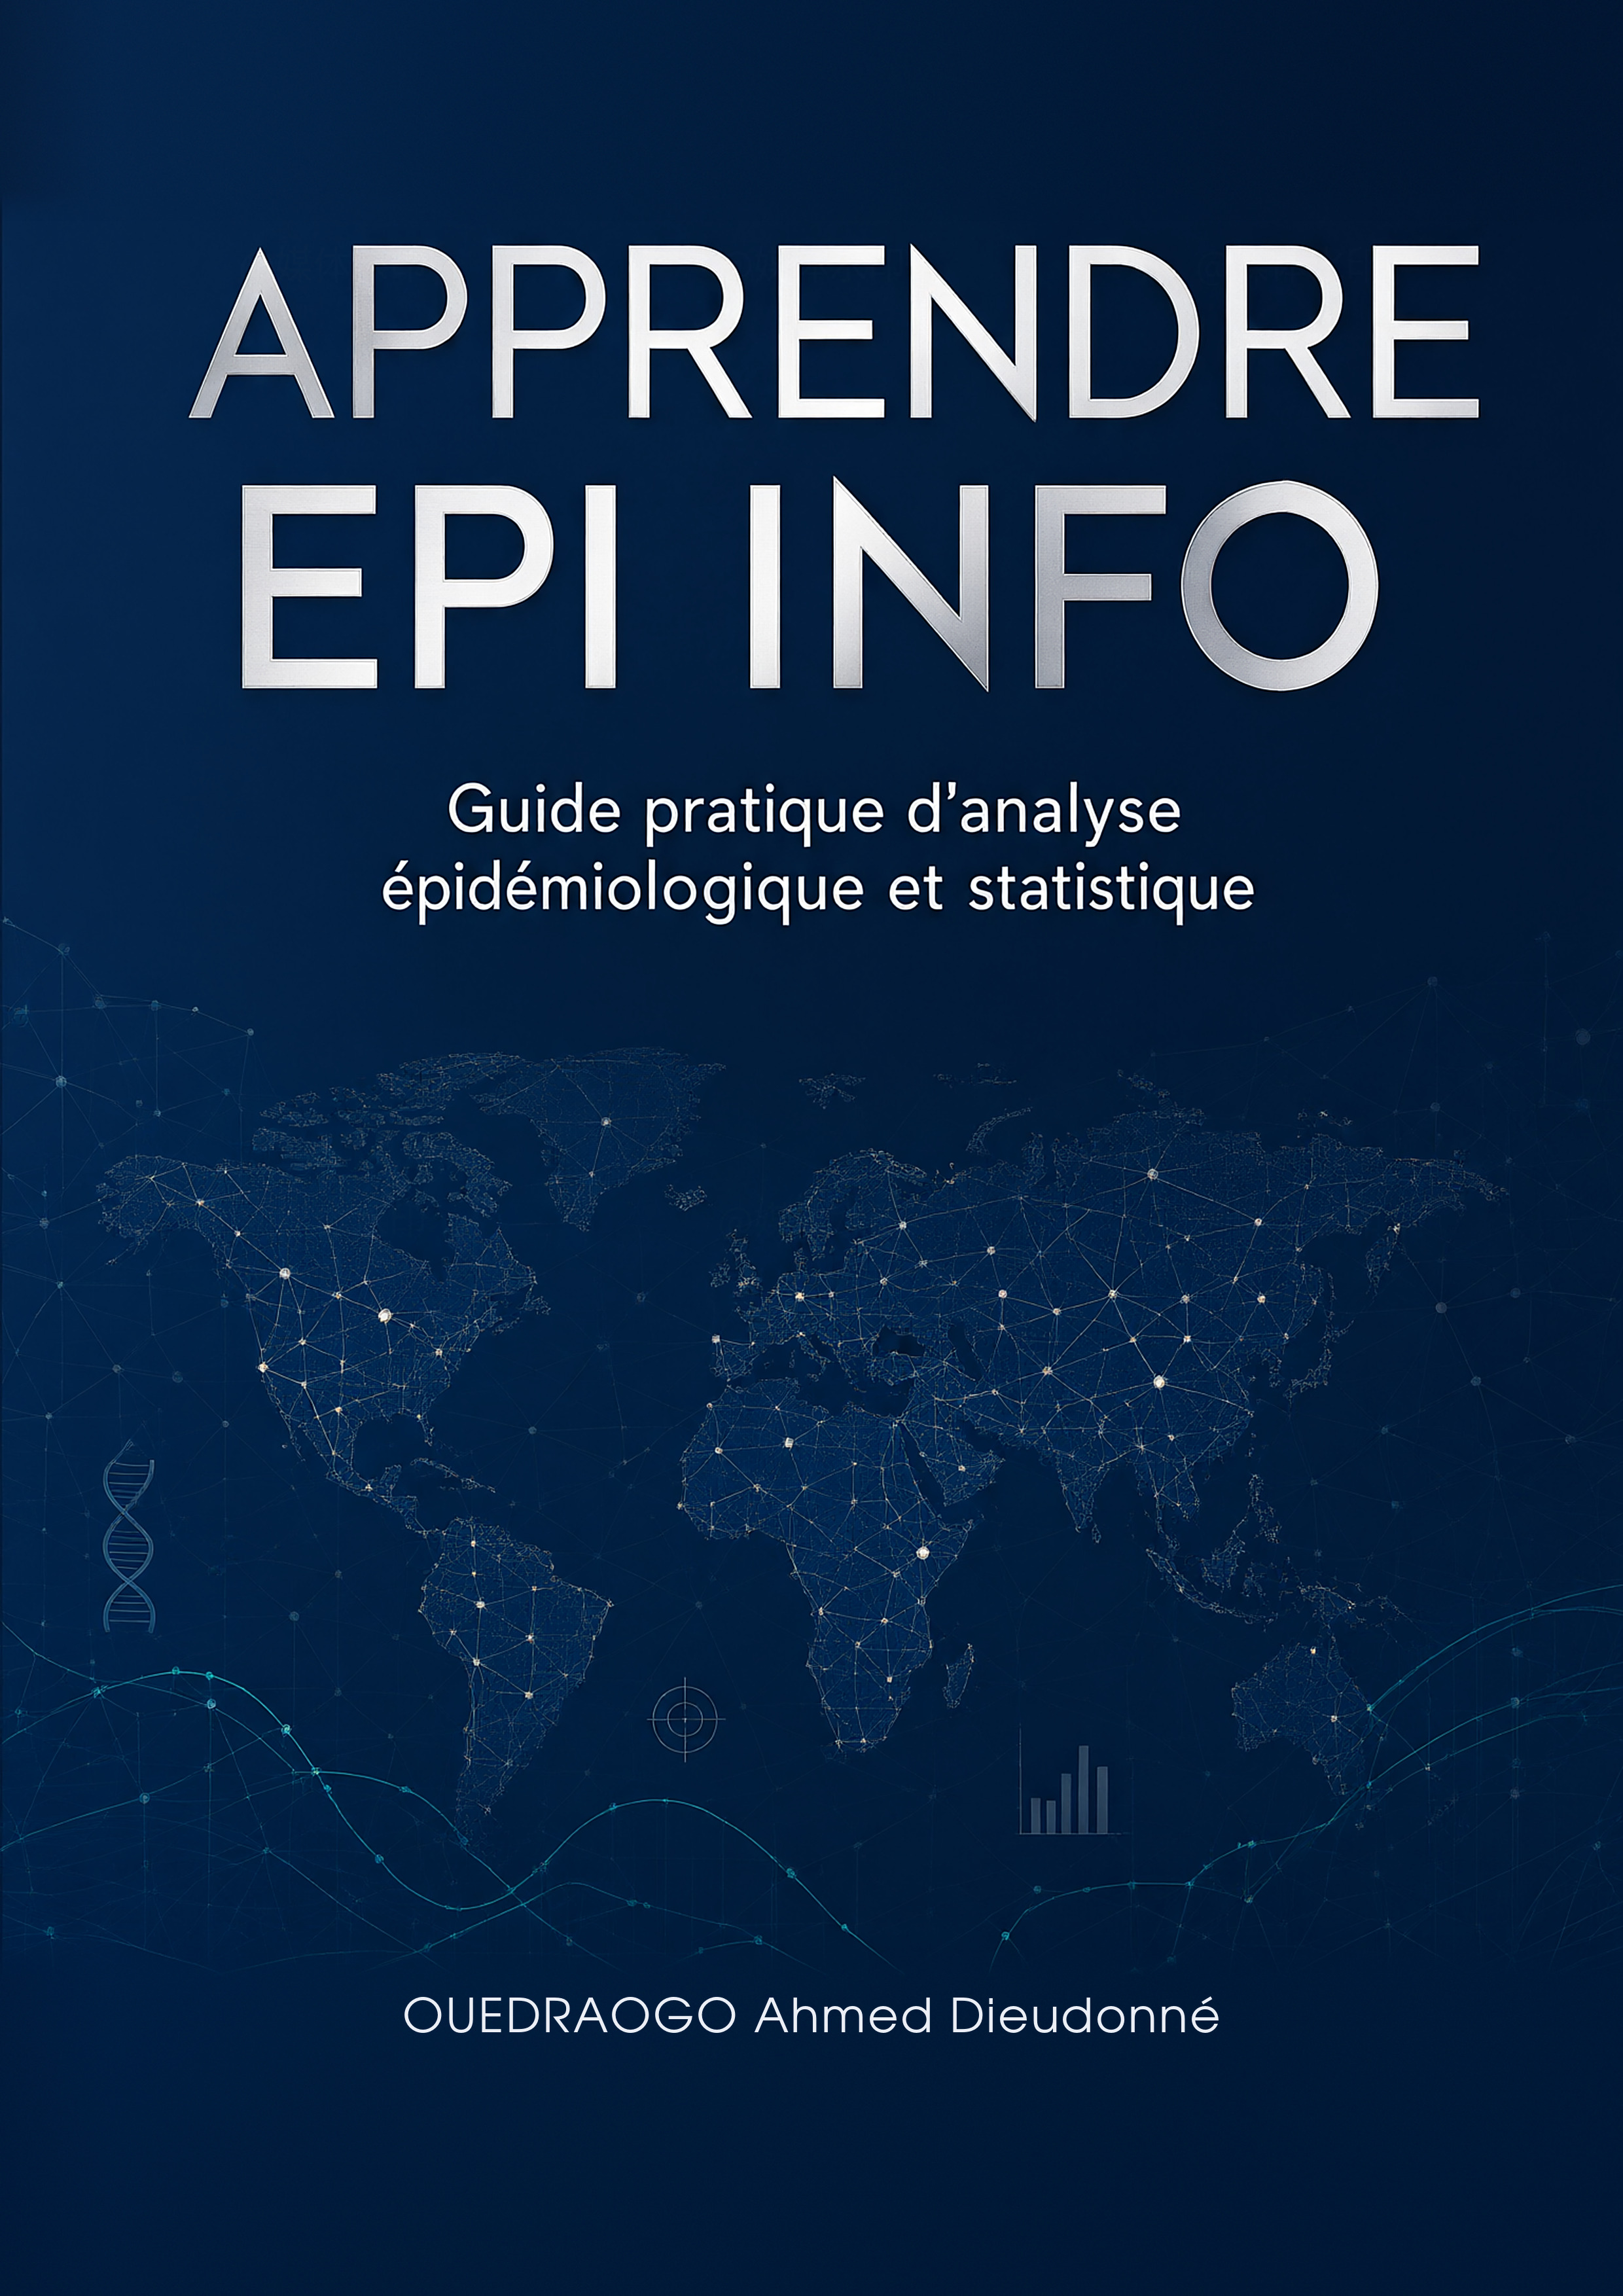
\includegraphics[width=\paperwidth,height=\paperheight]{img/couverture}};
\end{tikzpicture}
\clearpage

\chapter*{À propos de l'auteur}
\label{auteur}
\addcontentsline{toc}{chapter}{À propos de l'auteur}
\markboth{À propos de l'auteur}{À propos de l'auteur}

\textbf{OUEDRAOGO Ahmed Dieudonné} est médecin. C'est au cours de sa thèse de doctorat en médecine qu'il découvre Epi Info, en cherchant à analyser lui-même les données de son enquête. Ce premier contact avec l'analyse de données oriente durablement son parcours.

Data scientist, il s'intéresse à toutes les étapes du traitement des données de santé : conception des outils de collecte, nettoyage, analyse statistique, visualisation et automatisation des analyses. Il aime rendre ces méthodes accessibles au plus grand nombre, à commencer par des outils gratuits et simples d'utilisation comme Epi Info.

Consultant en e-santé, il accompagne la mise en place de solutions numériques pour la collecte et la gestion des données sanitaires, convaincu que des données de qualité sont la base de toute bonne décision en santé publique.

Il poursuit actuellement une formation d'épidémiologiste de terrain, centrée sur la surveillance épidémiologique, l'investigation des épidémies et la réponse aux urgences de santé publique. Sur le terrain, il mesure chaque jour combien un questionnaire bien conçu et une analyse rigoureuse comptent.

Ce livre est né de son expérience d'étudiant et de praticien. Il l'a écrit pour que d'autres étudiants, et tous les professionnels de santé qui débutent dans l'analyse de données, disposent du guide pratique en français qui lui avait manqué.

\vfill
\begin{center}
	\small
	© 2026 OUEDRAOGO Ahmed Dieudonné\\[0.5ex]
	Cet ouvrage est mis à disposition selon les termes de la licence\\
	\href{https://creativecommons.org/licenses/by-nc-sa/4.0/deed.fr}{Creative Commons Attribution -- Pas d'utilisation commerciale -- Partage dans les mêmes conditions 4.0 International (CC BY-NC-SA 4.0)}.\\[0.5ex]
	DOI : \href{https://doi.org/10.5281/zenodo.24182020}{10.5281/zenodo.24182020}
\end{center}


\tableofcontents
\clearpage
\listoffigures
\clearpage
\lstlistoflistings
\clearpage

\chapter*{Préambule}
\label{preambule}
\addcontentsline{toc}{chapter}{Préambule}
\markboth{Préambule}{Préambule}

J'ai écrit ce livre pour aider les étudiants en fin de cycle à se familiariser avec un outil qui leur permette d'analyser leurs données.

Lorsque j'étais étudiant en médecine, arrivé en fin de formation, j'ai été confronté à un problème épineux : l'analyse des données recueillies pour ma thèse de doctorat en médecine. Dans notre unité de formation, Epi Info était de très loin le logiciel le plus utilisé à cet effet. J'ai donc entrepris de me familiariser avec cet outil.

Ce livre est né d'un constat : les ressources documentaires en français étaient très limitées, même s'il existe un tutoriel rédigé par les concepteurs du logiciel.

\section*{Pourquoi le logiciel Epi Info ?}

Epi Info est un logiciel gratuit créé par les \emph{Centers for Disease Control and Prevention} (CDC), en français Centres pour le contrôle et la prévention des maladies, aux États-Unis. Il permet de concevoir des formulaires de saisie de données et de réaliser des analyses statistiques. Il est téléchargeable gratuitement sur le site du CDC. Sa courbe d'apprentissage est courte : même un néophyte peut le prendre en main très facilement.

Il faut toutefois noter quelques inconvénients. Epi Info 7 n'est pas multiplateforme : il a été conçu pour le système d'exploitation Windows de Microsoft\footnote{Notons néanmoins que Windows est le système d'exploitation le plus répandu sur les ordinateurs de bureau.}. Pour les représentations graphiques, bien que le logiciel le permette, nous les réaliserons en général dans un logiciel tiers comme Microsoft Excel ou LibreOffice Calc. De même, pour des analyses plus poussées, vous aurez besoin de logiciels plus puissants.

\section*{Organisation du livre}

Le livre suit les étapes d'une enquête, de la conception du questionnaire à l'analyse des données :
\begin{itemize}
	\item le chapitre~\ref{installationConfig} présente l'installation d'Epi Info 7 et son passage en français ;
	\item le chapitre~\ref{creerQuestionnaire} montre comment créer un questionnaire avec ses différents types de champs ;
	\item le chapitre~\ref{codeValidation} introduit le code de contrôle, qui rend le questionnaire plus robuste ;
	\item le chapitre~\ref{saisirDonnees} traite de la saisie des données ;
	\item les chapitres~\ref{moduleTableauDeBord} et~\ref{moduleClassic} sont consacrés à l'analyse statistique avec les modules \module{tableau de bord visuel} et \module{classique} ;
	\item le chapitre~\ref{moduleStatcalc} présente le module \module{statcalc}, qui permet de calculer la taille d'un échantillon et d'analyser rapidement des tableaux déjà constitués.
\end{itemize}

Au fil de ce livre, vous apprendrez progressivement à créer un formulaire robuste et cohérent, puis à analyser vos données avec ce logiciel.

Je vous souhaite une bonne lecture.


\mainmatter
\chapter{Installation et configuration d'Epi Info 7}
\label{installationConfig}

Dans ce chapitre, nous allons télécharger le logiciel Epi Info sur le site internet du CDC, à l'adresse {\footnotesize \url{https://www.cdc.gov/epiinfo/support/downloads.html}}, puis l'installer sur notre ordinateur et l'afficher en français.

\section{Configuration requise}

Epi Info 7 fonctionne sous Microsoft Windows 7 ou une version plus récente et nécessite le composant Microsoft .NET Framework 4.8, déjà présent sur les versions récentes de Windows. La version utilisée dans ce livre est la version~7.2 ; les captures d'écran ont été réalisées avec la version~7.2.5.

\begin{mybox}[colbacktitle=NOTE]{\faInfoCircle{} À RETENIR}
Le CDC a annoncé l'arrêt du développement et de l'assistance technique d'Epi Info à partir du 1\ier{} septembre 2025. La dernière version reste téléchargeable et utilisable gratuitement, mais elle ne recevra plus de mises à jour.
\end{mybox}

\section{Télécharger et installer Epi Info 7}

Le logiciel est distribué sous la forme d'un fichier compressé (\var{.zip}) qui ne demande pas d'installation classique. Pour l'installer :

\begin{enumerate}
	\item Ouvrir la page de téléchargement indiquée plus haut et cliquer sur le lien de téléchargement du fichier ZIP d'Epi Info 7 ;
	\item Une fois le téléchargement terminé, faire un clic droit sur le fichier compressé puis choisir \kw{Extraire tout\ldots} ;
	\item Choisir un emplacement facile à retrouver, par exemple \var{C:\textbackslash Epi Info 7}, puis valider. Évitez de laisser le dossier dans \var{Téléchargements} ;
	\item Ouvrir le dossier extrait et double-cliquer sur le fichier \var{Launch Epi Info 7.exe} pour lancer le logiciel ;
	\item Pour retrouver facilement le logiciel, faire un clic droit sur ce fichier puis \kw{Envoyer vers > Bureau (créer un raccourci)}.
\end{enumerate}

\begin{mybox}[colbacktitle=TIP]{\faLightbulb{} CONSEIL}
Au premier lancement, Windows peut afficher un avertissement de sécurité. Après avoir vérifié que le fichier provient bien du site du CDC, cliquez sur \kw{Informations complémentaires} puis sur \kw{Exécuter quand même}.
\end{mybox}

\section{Mettre Epi Info en français}

Lorsque nous lançons Epi Info pour la première fois, il s'affiche comme sur la \autoref{fig:epiintro}.

\begin{figure}[H]
	\centering
	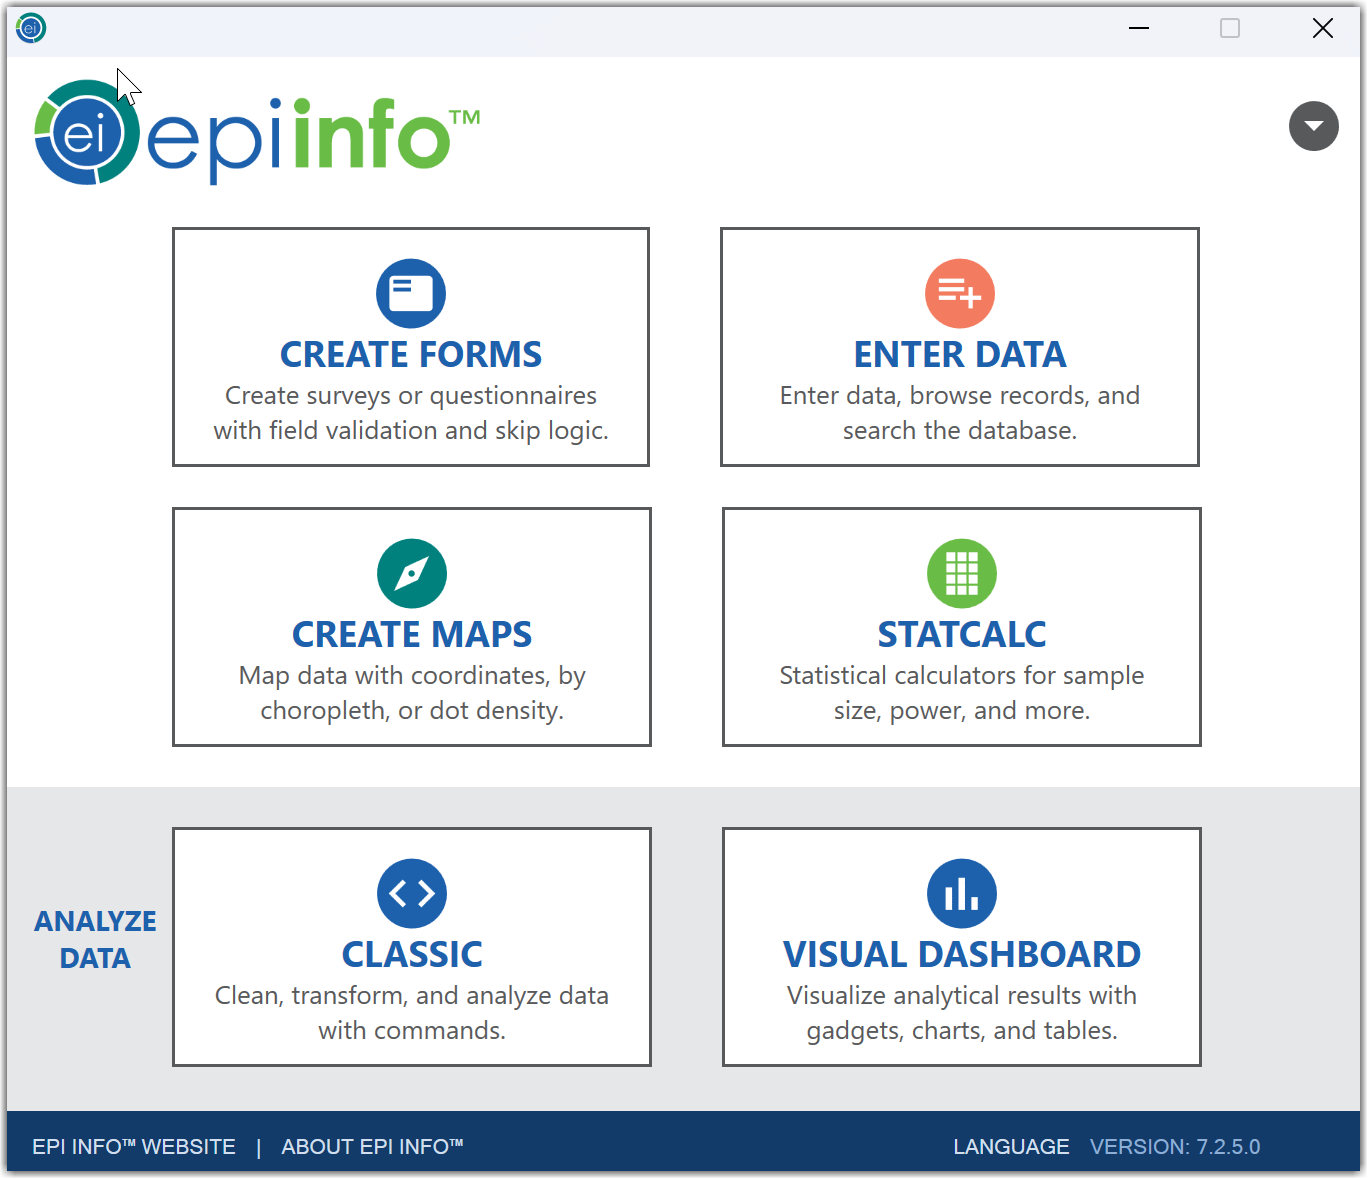
\includegraphics[width=.85\linewidth]{img/config/epiintro}
	\caption{Fenêtre d'accueil d'Epi Info 7}
	\label{fig:epiintro}
\end{figure}

Nous remarquons que le logiciel s'affiche en anglais. Pour le passer en français :

\begin{enumerate}
	\item Cliquer en bas à droite de la fenêtre d'accueil sur \kw{\textsc{language}} ;
	\item Dans la fenêtre qui s'ouvre, choisir \kw{French (France)} ;
	\item Cliquer sur \kw{Apply} pour appliquer le changement ;
	\item Fermer puis relancer le logiciel.
\end{enumerate}

Epi Info s'affiche désormais en français. Dans la suite de ce livre, les noms des menus et des boutons sont donc donnés en français. Certains éléments restent toutefois en anglais même après ce changement ; nous les signalerons au fur et à mesure.

\chapter{Créer les champs d'un questionnaire}
\label{creerQuestionnaire}
%\minitoc

La création d'un questionnaire, ou formulaire, est une étape très importante dans la conduite d'une enquête. Vous devez au préalable élaborer votre plan de recueil des données et préparer vos questions. Dans le cadre d'un mémoire ou d'une thèse, ce travail se prépare en amont avec votre directeur ou directrice de mémoire ou de thèse, et le questionnaire doit figurer dans votre protocole de recherche. Nous allons maintenant apprendre à créer des questionnaires avec Epi Info 7.

Lançons Epi Info 7, qui s'affiche désormais en français. Le logiciel comporte plusieurs modules :
\begin{itemize}
	\item \module{créer questionnaires}, qui, comme son nom l'indique, permet de créer des questionnaires ;
	\item \module{saisir des données}, pour saisir les données ;
	\item \module{créer des cartes}, pour cartographier les données ;
	\item \module{statcalc}, pour le calcul de la taille des échantillons ;
	\item \module{classique} et \module{tableau de bord visuel}, pour l'analyse statistique des données.
\end{itemize}
Cliquons sans tarder sur le module \module{créer questionnaires} (\autoref{fig:creerquestionnaire}).

\begin{figure}[H]
	\centering
	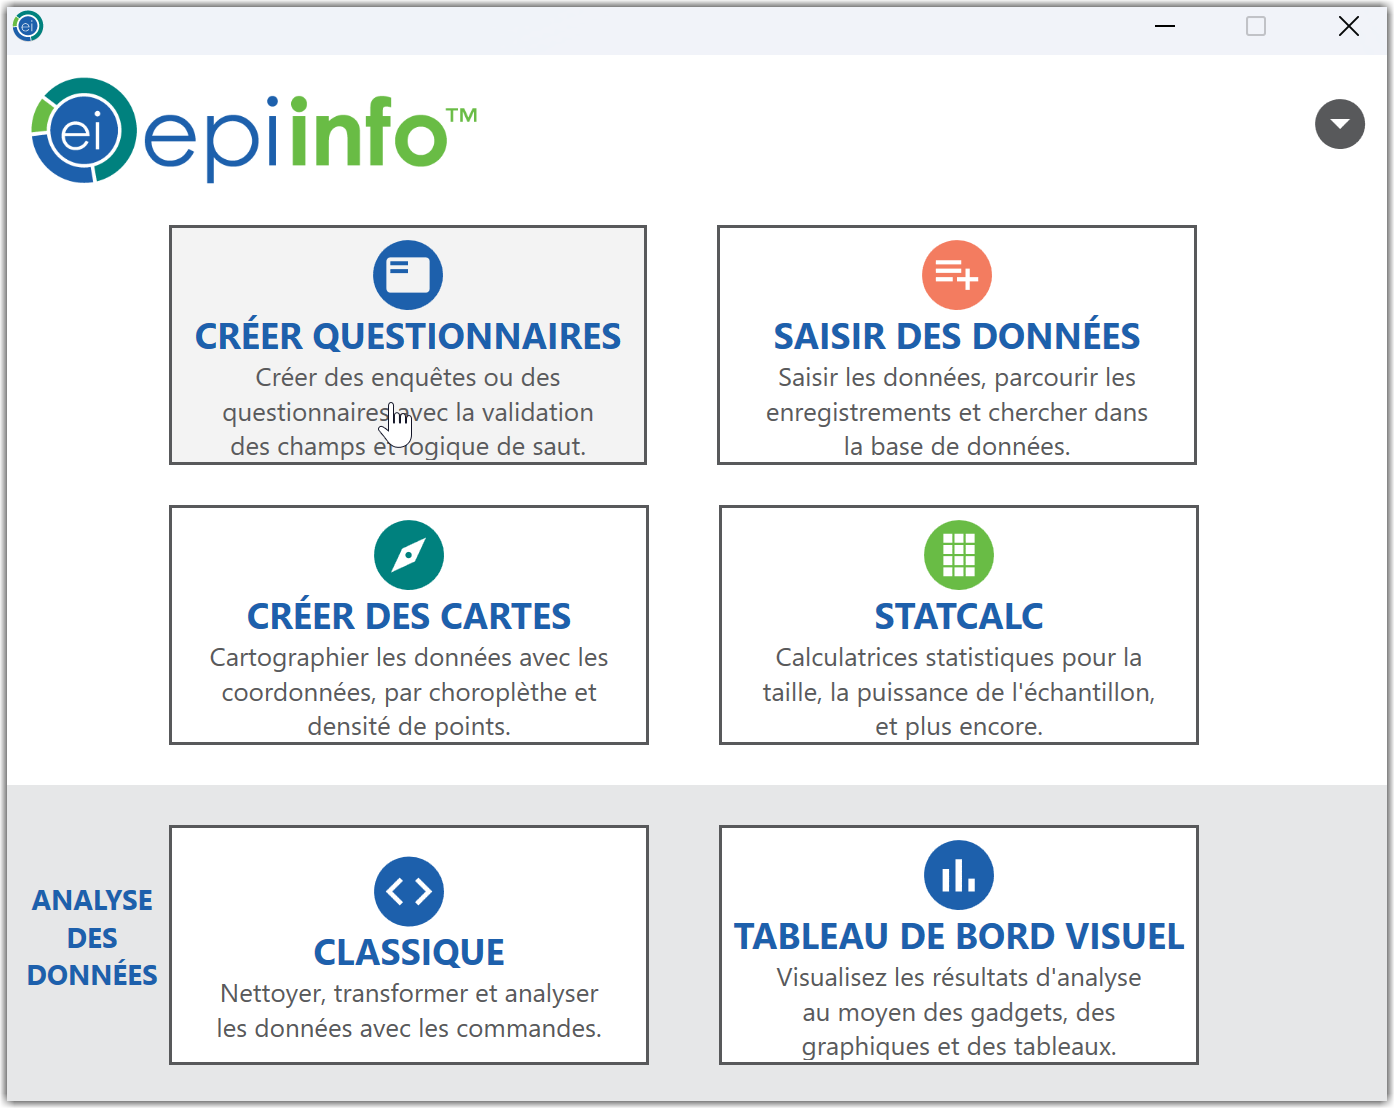
\includegraphics[width=\linewidth,height=0.4\textheight,keepaspectratio]{img/questionnaire/creerQuestionnaire}
	\caption{Module Créer questionnaires}
	\label{fig:creerquestionnaire}
\end{figure}

\section{Créer un projet}
\label{creerProjet}

Une fois dans le module \module{créer questionnaires}, nous allons créer un projet qui contiendra notre ou nos formulaires. En effet, un même projet peut contenir plusieurs formulaires d'une enquête.

Après avoir cliqué sur l'onglet \kw{Nouveau projet}, une fenêtre s'ouvre avec des champs à remplir. Nous saisissons le nom du projet, une description si besoin et enfin le nom du formulaire. Ici, nous avons choisi de nommer notre projet COVID19 : le nom doit être écrit d'un seul tenant, sans espace ni caractère spécial. Dans la partie \kw{Données}, le format proposé par défaut est \kw{Microsoft Access 2002-2003 (.mdb)}. Nous le conservons ; on pourrait aussi choisir \kw{Microsoft SQL Server Database} ou tout autre système que l'on maîtrise bien. Nous validons ensuite la création du projet par \kw{OK} (\autoref{fig:nouveauprojet}).

\begin{figure}[H]
	\centering
	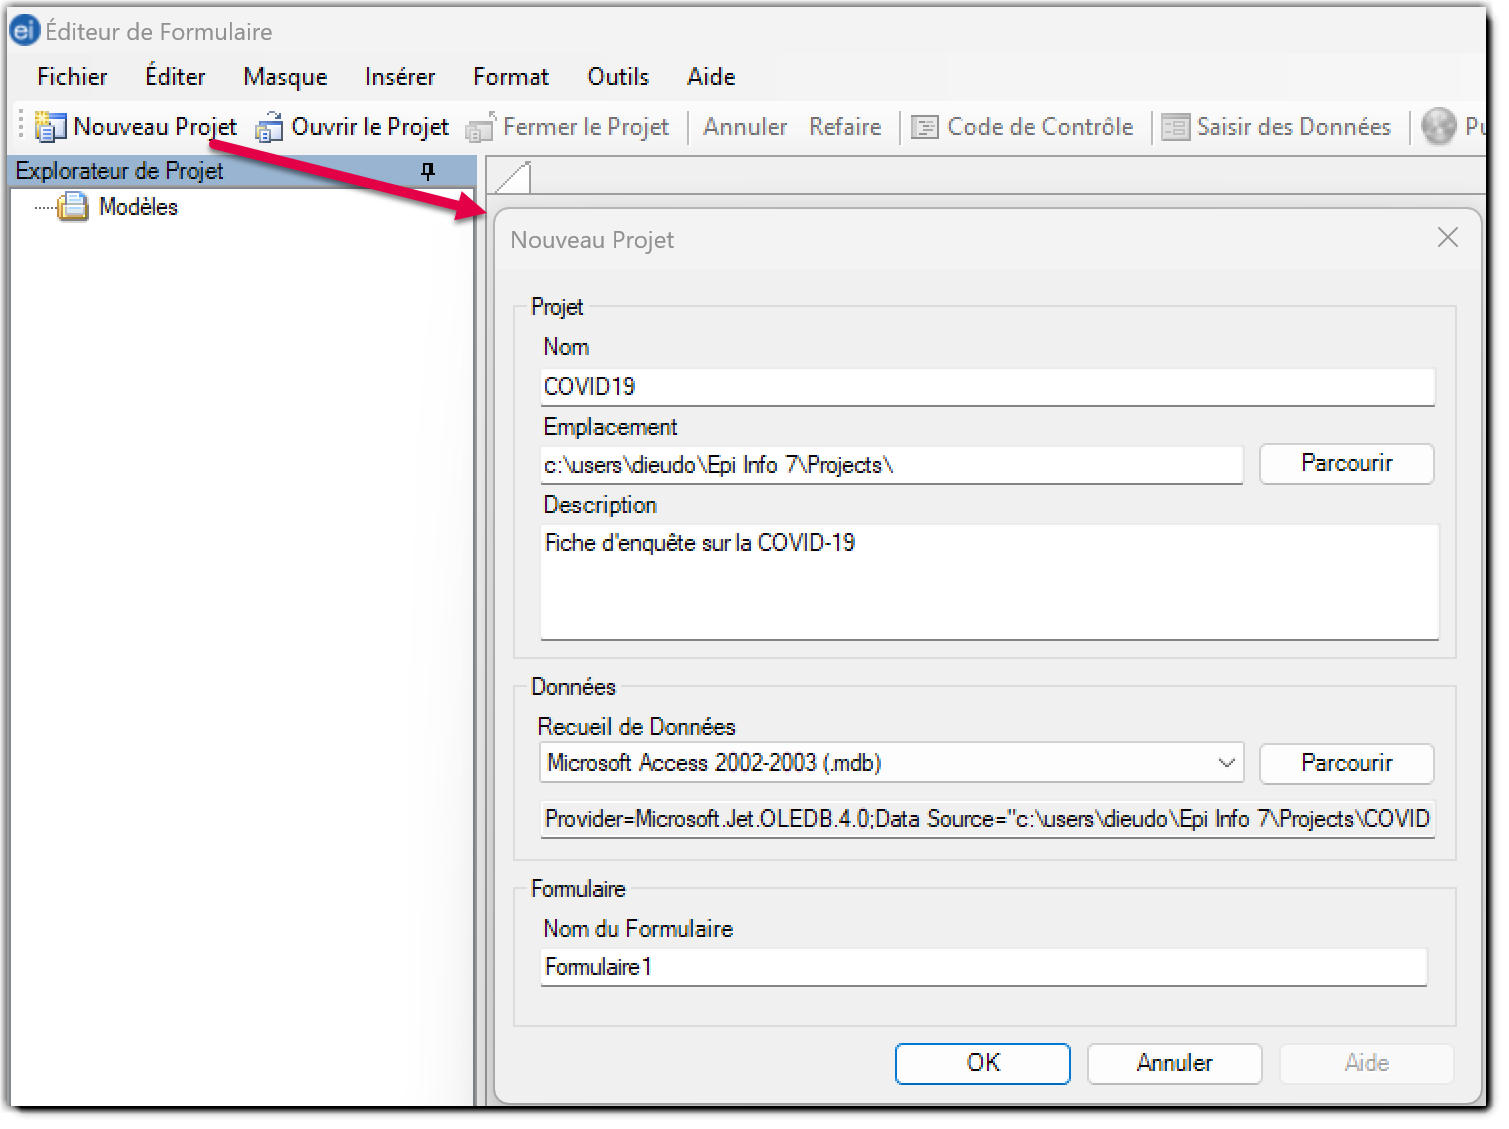
\includegraphics[width=\linewidth,height=0.4\textheight,keepaspectratio]{img/questionnaire/nouveauProjet}
	\caption{Créer un nouveau projet}
	\label{fig:nouveauprojet}
\end{figure}

Une nouvelle fenêtre s'ouvre alors et nous pouvons éditer notre formulaire. Elle présente trois parties : la barre d'outils, l'explorateur de projets et le canevas (\autoref{fig:menuaccueilprojet}).

\begin{figure}[H]
	\centering
	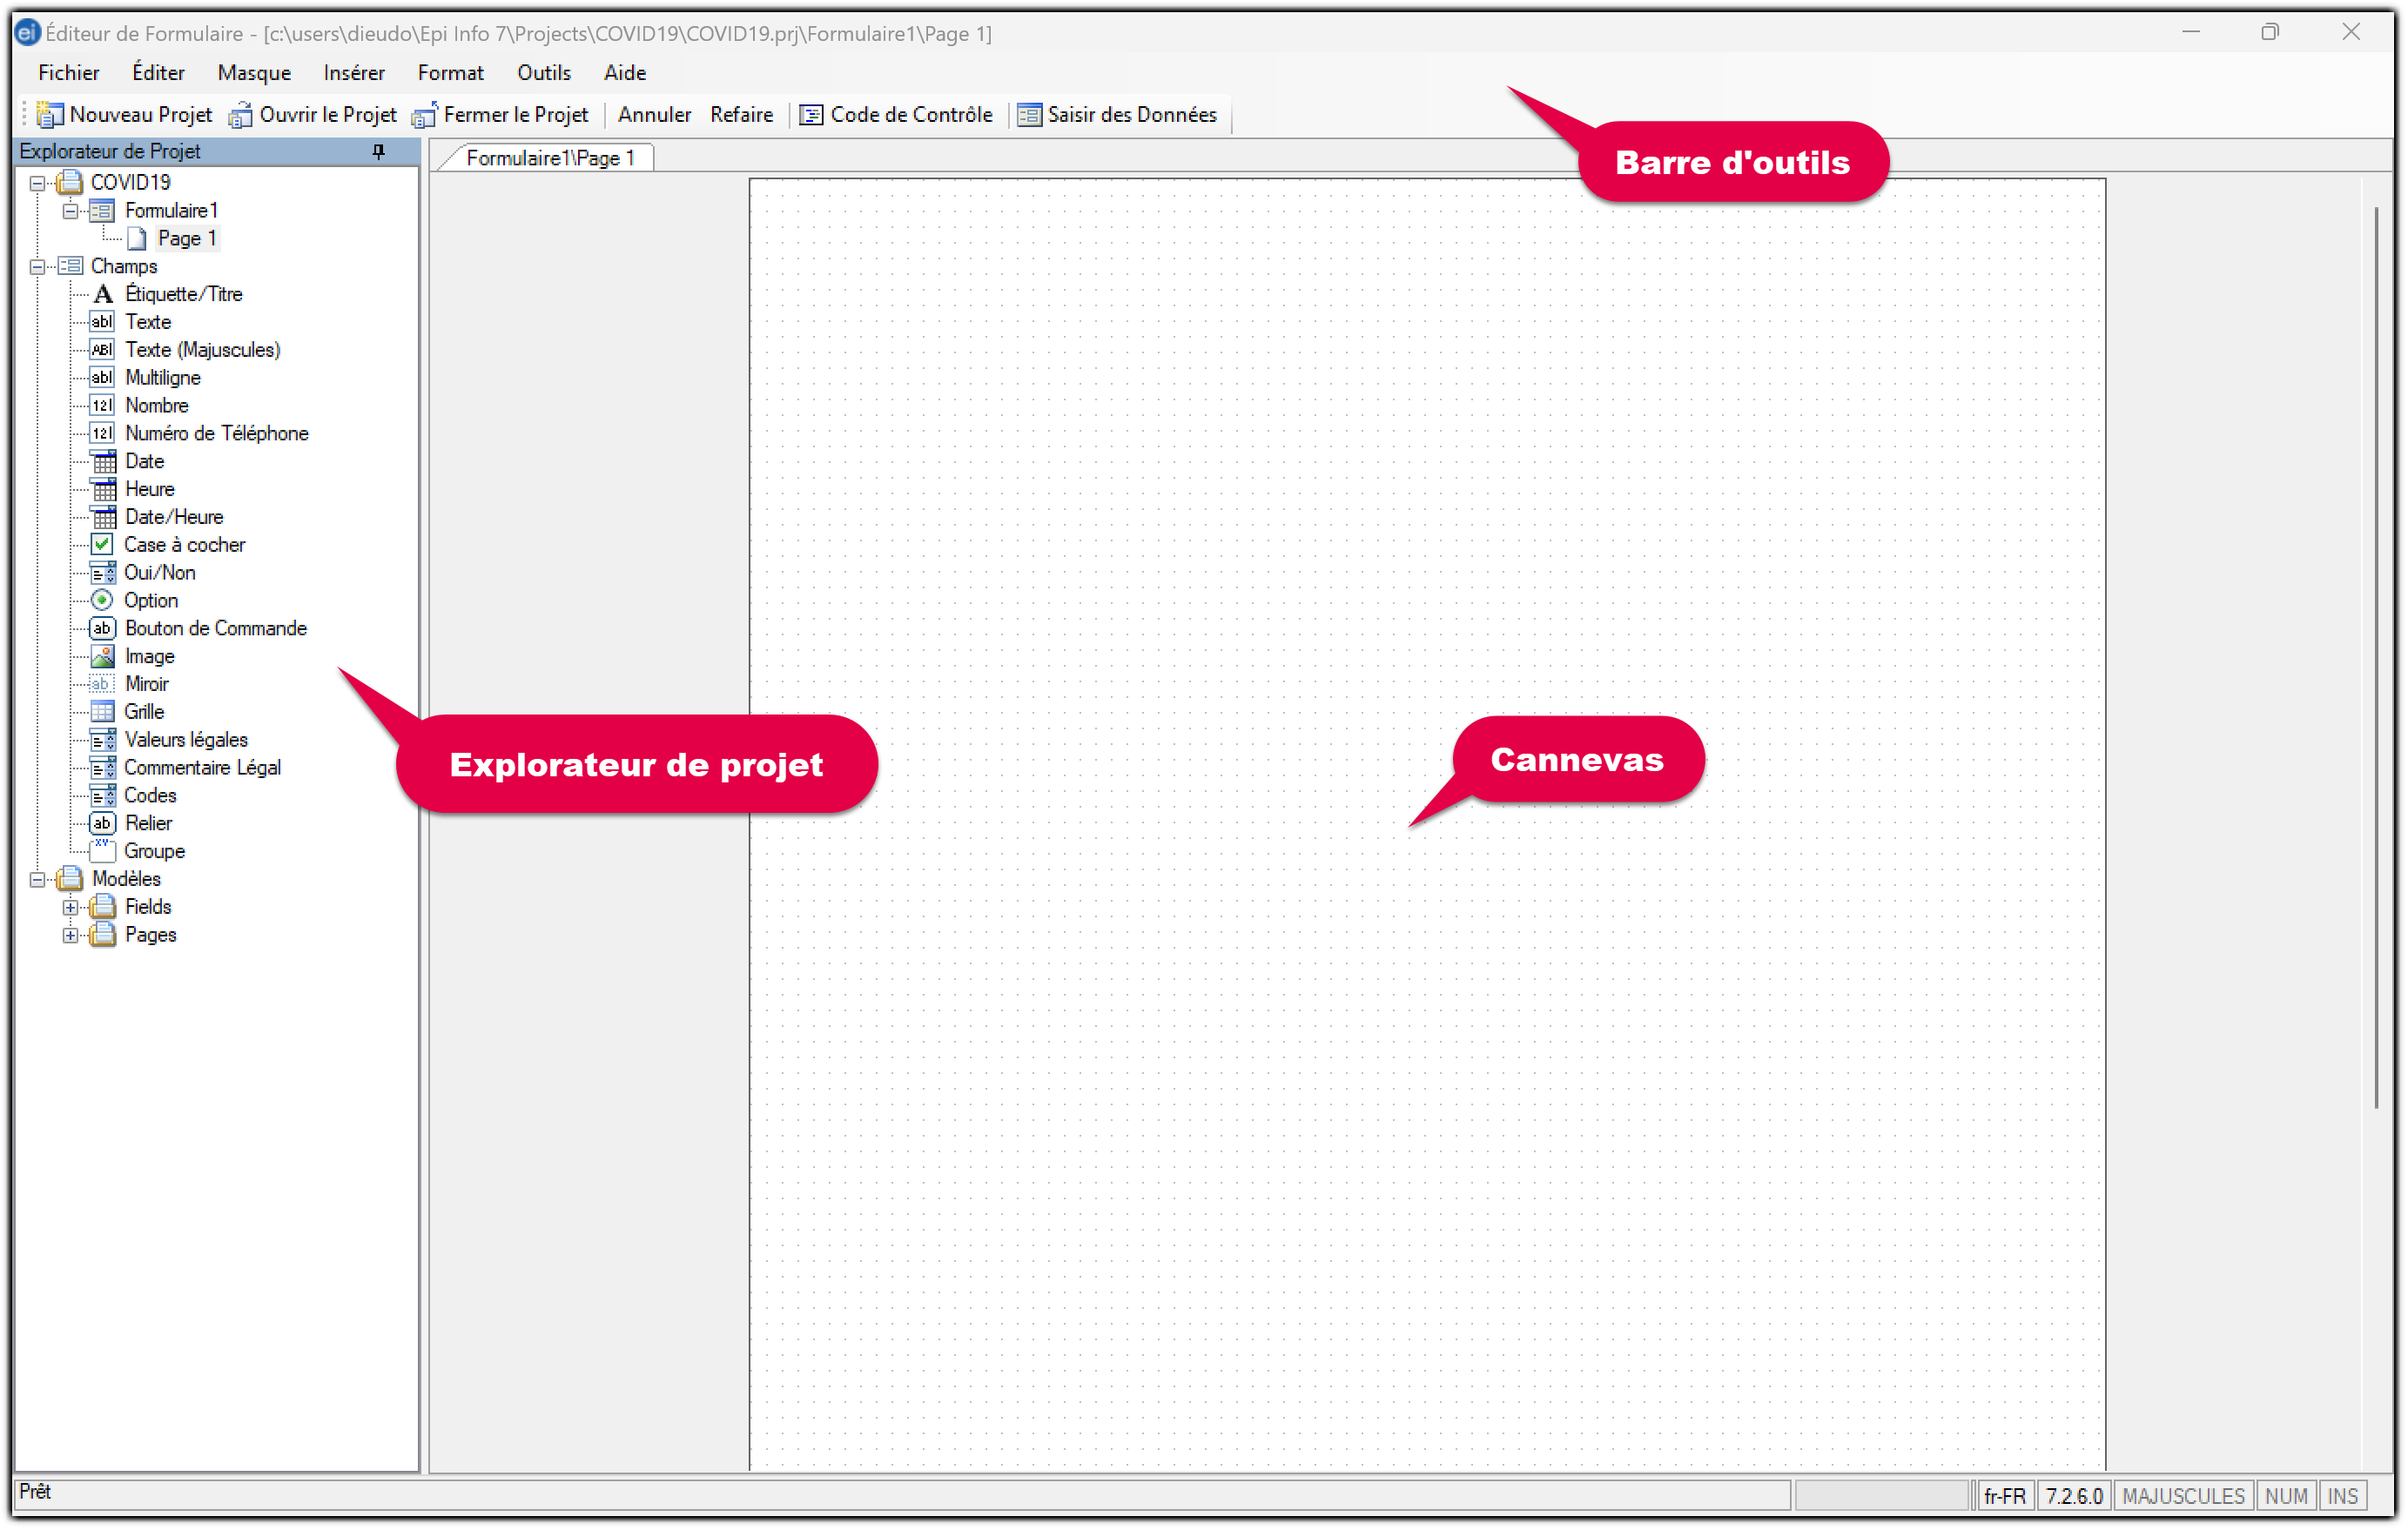
\includegraphics[width=\linewidth,height=0.4\textheight,keepaspectratio]{img/questionnaire/menuAccueilProjet}
	\caption{Page d'accueil de notre projet}
	\label{fig:menuaccueilprojet}
\end{figure}

Une fois le projet créé, nous allons créer les champs de notre questionnaire.

\section{Règles de nommage des variables}
\label{typo}

Pour nommer nos variables, nous utiliserons une convention d'écriture : le \emph{camel case} ou le \emph{snake case}.

Le \emph{camel case}\footnote{Littéralement \og casse de chameau \fg{}. Cette façon d'écrire est aussi devenue une mode : le marketing en a tiré de nombreuses marques, comme MasterCard, PlayStation ou iPhone.} consiste à écrire un ensemble de mots en les liant sans espace ni ponctuation, et en mettant en capitale la première lettre de chaque mot. La première lettre du premier mot peut être en minuscule ou en majuscule. Par exemple : satisfactionClient ou SatisfactionClient (\autoref{fig:camelcase}).

\begin{figure}[H]
	\centering
	\begin{minipage}{0.45\linewidth}
		\centering
		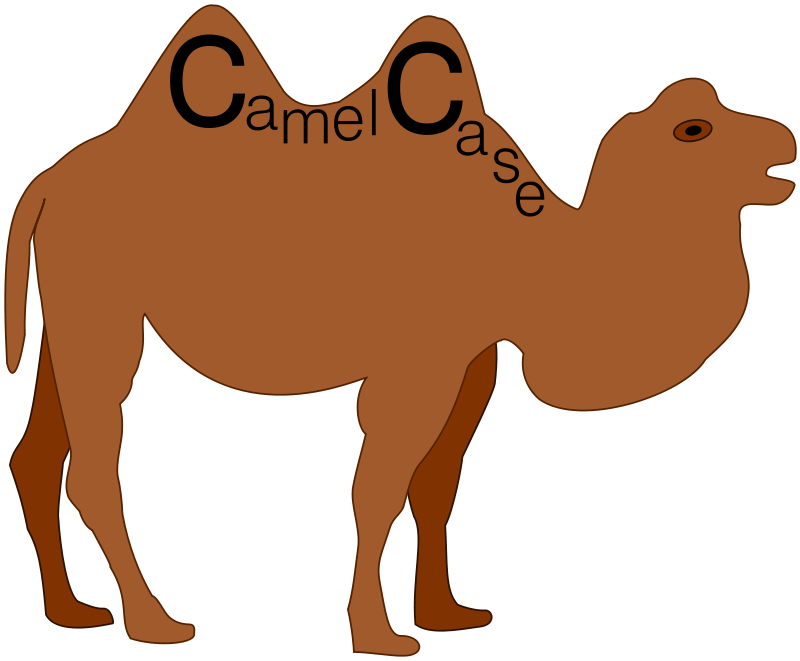
\includegraphics[width=\linewidth]{img/typo/CC}
	\end{minipage}\hfill
	\begin{minipage}{0.45\linewidth}
		\centering
		
\includegraphics[width=\linewidth]{img/typo/camelC}
	\end{minipage}
	\caption{Le camel case : première lettre en majuscule (à gauche) ou en minuscule (à droite)}
	\label{fig:camelcase}
\end{figure}

Le \emph{snake case}\footnote{Il utilise le tiret bas \og \_ \fg{}, comme dans mon\_premier\_chapitre.} consiste quant à lui à écrire les mots, généralement en minuscules, en les séparant par des tirets bas. Ces deux conventions ne sont pas les seules possibles, mais ce sont les plus répandues.

\begin{mybox}[colbacktitle=IMPORTANT]{\faExclamationCircle{} IMPORTANT}
	\begin{itemize}[label=\ding{97}, font=\color{IMPORTANT}]
	\item Utiliser le camel case ou le snake case pour les noms de variables ;
	\item Éviter les noms très longs ;
	\item Employer des noms explicites : revenuAnnuel ou revenu\_annuel plutôt que revAnnuel ou rev\_annuel ;
	\item Ne pas commencer un nom de variable par un chiffre ;
	\item Ne pas utiliser les mots réservés du logiciel. Un mot réservé se reconnaît à sa coloration rouge ; heureusement, Epi Info désactive la création du champ si un mot réservé est utilisé.
\end{itemize}
\end{mybox}

\section{Comment ajouter un champ}

Il existe plusieurs types de champs selon le type de variable à recueillir : texte, nombre, date, case à cocher, valeurs légales, etc. Il y a trois façons d'ajouter un champ :

\begin{itemize}
\item double-cliquer sur le type de champ voulu dans l'explorateur de projets ;
\item faire un glisser-déposer : cliquer sur le type de champ, maintenir le bouton de la souris enfoncé et déposer le champ sur le canevas ;
\item faire un clic droit sur le canevas, puis choisir le type de champ voulu dans le menu \kw{Nouveau champ}.
\end{itemize}

C'est la première méthode, le double-clic, que nous utiliserons dans ce livre pour nos illustrations.

\section{Ajouter une étiquette}

Pour débuter notre questionnaire, nous avons besoin d'un titre. Pour le créer, nous procédons comme suit :
\begin{enumerate}
	\item Double-cliquer sur \kw{Étiquette/Titre} dans l'explorateur de projets ;
	\item Une fenêtre nommée Étiquette/Titre s'ouvre ;
	\item Saisir dans le champ \kw{Question ou Invite} le titre du questionnaire, ici \question{Enquête Covid-19} ;
	\item Appuyer sur la touche de tabulation du clavier. Le curseur passe dans le champ \kw{Nom du champ} et le remplit automatiquement à partir de ce que vous avez saisi dans l'invite ;
	\item Vérifier le nom du champ proposé et le corriger si besoin, conformément aux règles de nommage (section~\ref{typo}). Remarquez qu'Epi Info supprime les lettres accentuées : pour notre titre, il propose \var{Enqute\_Covid19} ;
	\item Valider par \kw{OK} (\autoref{fig:ajoutetiquette}).
\end{enumerate}

\begin{mybox}[colbacktitle=TIP]{\faLightbulb{} CONSEIL}
Cliquez sur le bouton \kw{Police}, en bas de la fenêtre, pour changer de police, augmenter la taille des caractères ou mettre le titre en gras.
\end{mybox}

\begin{figure}[H]
	\centering
	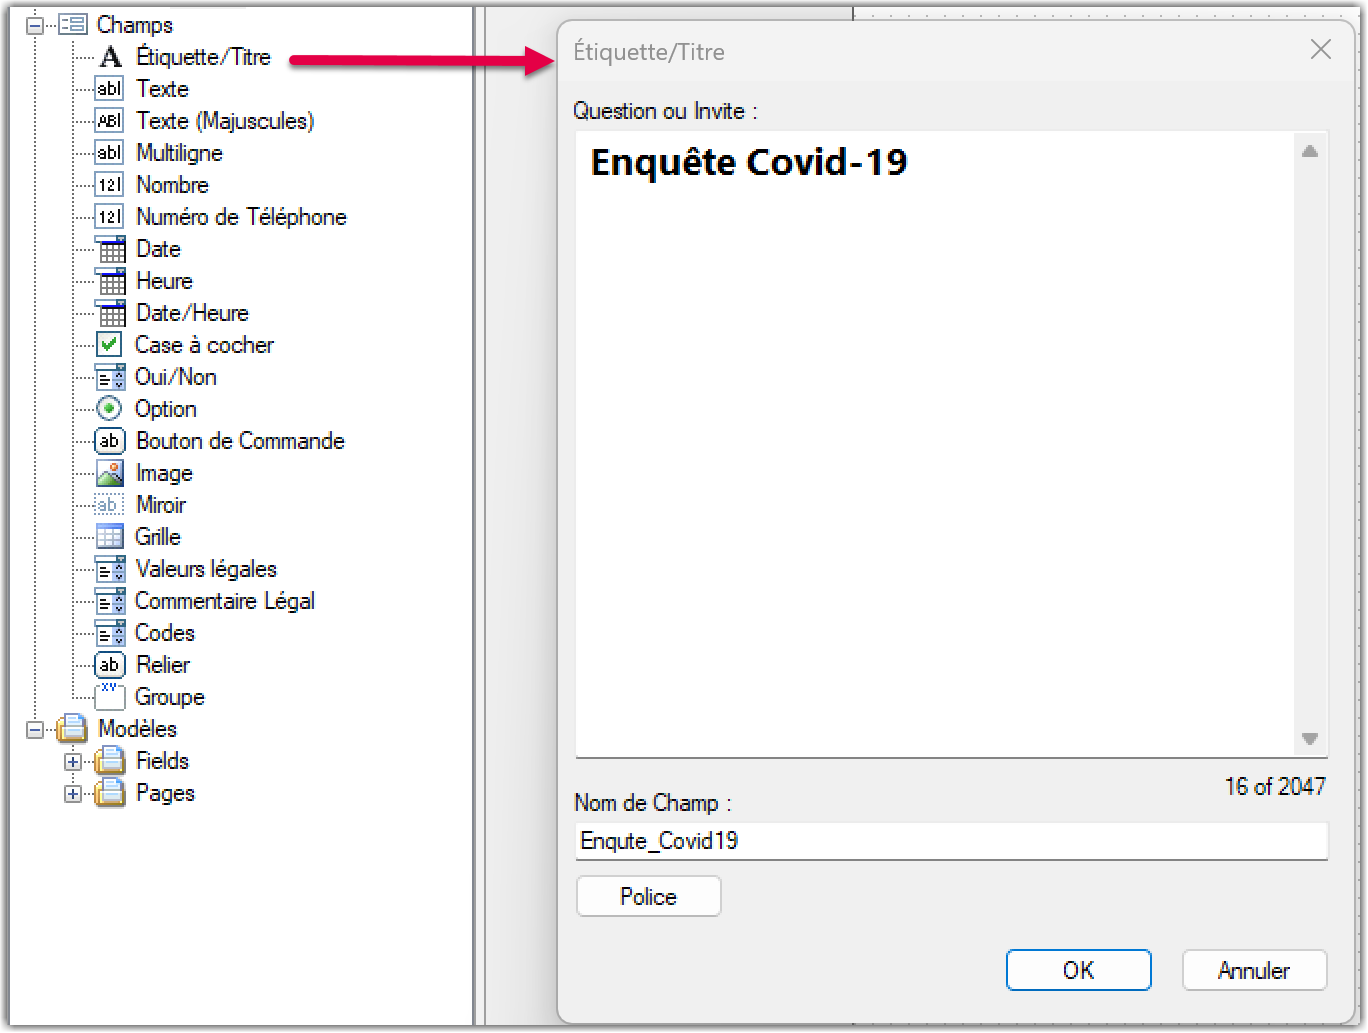
\includegraphics[width=\linewidth,height=0.4\textheight,keepaspectratio]{img/questionnaire/ajoutEtiquette}
	\caption{Ajouter une étiquette}
	\label{fig:ajoutetiquette}
\end{figure}

Utilisez la souris pour placer le texte sur le canevas. Pour modifier ensuite le titre ou la taille de la police, faites un clic droit sur le champ puis choisissez \kw{Propriétés} : vous retrouvez la fenêtre initiale.

\section{Ajouter un champ de type texte}

Un champ texte est un champ dans lequel on écrit du texte libre : nom, prénom, adresse, etc.
Pour ajouter un champ de type texte, procéder comme suit :

\begin{enumerate}
	\item Double-cliquer sur \kw{Texte} dans l'explorateur de projets ;
	\item Une fenêtre nommée Texte s'ouvre ;
	\item Taper \kw{Nom} dans le champ \kw{Question ou Invite}. C'est ce libellé qui s'affichera sur le questionnaire : c'est l'étiquette de la question ;
	\item Appuyer sur la touche de tabulation. Le curseur passe dans le champ \kw{Nom du champ} et le remplit automatiquement à partir de l'invite ;
	\item Réécrire le nom du champ, qui correspond au nom de la variable, conformément aux règles de nommage ;
	\item Dans les attributs, cocher \kw{Requis} rend le champ obligatoire. Réfléchissez-y avant de cocher cette case ;
	\item Valider par \kw{OK} (\autoref{fig:ajoutchamptexte}).
\end{enumerate}

\begin{mybox}[colbacktitle=CAUTION]{\faFire{} AVERTISSEMENT}
Par défaut, Epi Info construit le nom de la variable à partir du texte saisi dans le champ Question ou Invite. Il faut donc corriger le nom du champ pour obtenir un nom de variable cohérent, comme vu à la section~\ref{typo}, \nameref{typo}, page~\pageref{typo}.
\end{mybox}

Nous procédons de la même façon avec les champs \kw{Texte (Majuscules)} et \kw{Multiligne}. Comme le champ \kw{Texte}, ce sont des champs dans lesquels on saisit du texte brut.

\begin{figure}[H]
	\centering
	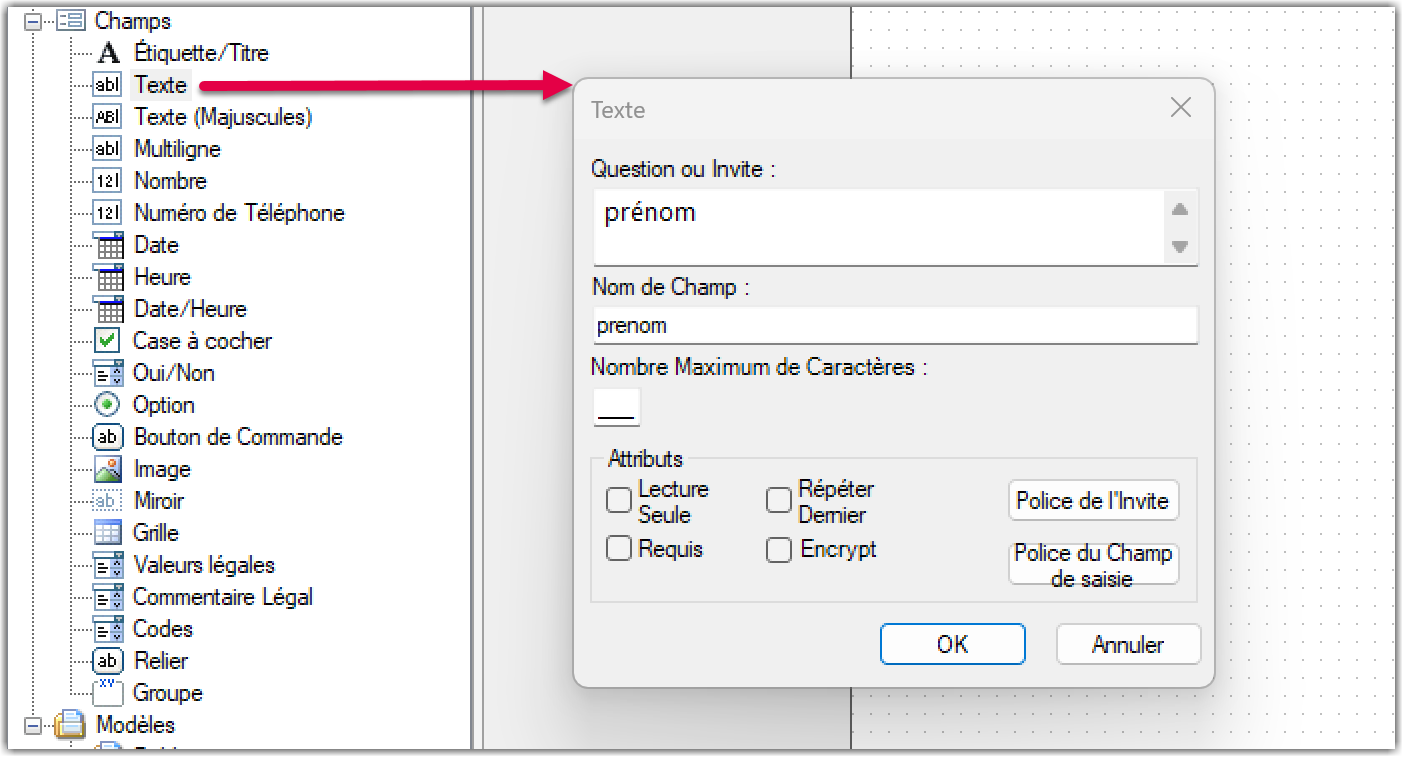
\includegraphics[width=\linewidth,height=0.4\textheight,keepaspectratio]{img/questionnaire/ajoutChampTexte}
	\caption{Ajouter un champ de type Texte}
	\label{fig:ajoutchamptexte}
\end{figure}

\section{Ajouter un champ de type numérique}
\label{champNumerique}

Dans un champ texte, l'utilisateur peut saisir n'importe quelle valeur. Ce type de champ ne convient donc pas pour recueillir certaines données comme l'âge ou la température d'un patient au moment de l'entretien.
Un champ numérique garantit que seuls des nombres valides sont acceptés. C'est indispensable lors de l'analyse, par exemple pour calculer une moyenne, une médiane, un mode ou les valeurs minimale et maximale.

Les champs de type numérique sont les champs \kw{Nombre} et \kw{Numéro de téléphone}. Prenons l'exemple du champ Nombre avec la variable âge :

\begin{enumerate}
	\item Double-cliquer sur \kw{Nombre} dans l'explorateur de projets. Une fenêtre nommée Nombre apparaît ;
	\item Dans le champ \kw{Question ou Invite}, écrire \og Âge \fg{} ;
	\item Appuyer sur la touche de tabulation. Le curseur passe dans le champ \kw{Nom du champ} et le remplit automatiquement à partir de l'invite ;
	\item Corriger le nom du champ, ici \var{age} ;
	\item Dans la liste déroulante \kw{Modèle}, sélectionner \#\#\#\footnote{\#\#\# signifie que la valeur comporte au plus trois chiffres entiers ; \#\#.\#\# signifie deux chiffres entiers et deux chiffres après la virgule. Le point entre les dièses correspond à la virgule dans la notation anglaise.} ;
	\item Cocher l'attribut \kw{Lecture seule} si l'âge doit être calculé automatiquement à partir de la date de naissance et de la date de l'enquête. Nous verrons comment au chapitre~\ref{codeValidation}, \nameref{codeValidation}, page~\pageref{codeValidation}.
\end{enumerate}

De la même façon, nous créons les champs \var{poids\_kg} et \var{taille\_cm} avec le modèle \#\#\# (trois dièses) : chez l'être humain, la taille en centimètres comme le poids en kilogrammes ne dépassent pas trois chiffres.

Nous pouvons limiter les erreurs de saisie en définissant un intervalle de valeurs acceptables. Pour le champ \var{taille\_cm}, cocher la case \kw{Intervalle} puis remplir les bornes inférieure et supérieure, ici respectivement 0 et 300 (\autoref{fig:ajoutchampnombre}). Nous supposons ici qu'une taille humaine est comprise entre 0 et 300~cm ; vous ajusterez ces bornes en fonction de votre public cible.

Nous créons enfin un champ numérique nommé \var{imc}. La procédure est la même, mais nous cochons l'attribut \kw{Lecture seule} : nous ne voulons pas calculer l'IMC à la main, mais le faire déduire automatiquement du poids et de la taille. Nous verrons comment programmer ce calcul au chapitre~\ref{codeValidation}, \nameref{codeValidation}, page~\pageref{codeValidation}.

\begin{figure}[H]
	\centering
	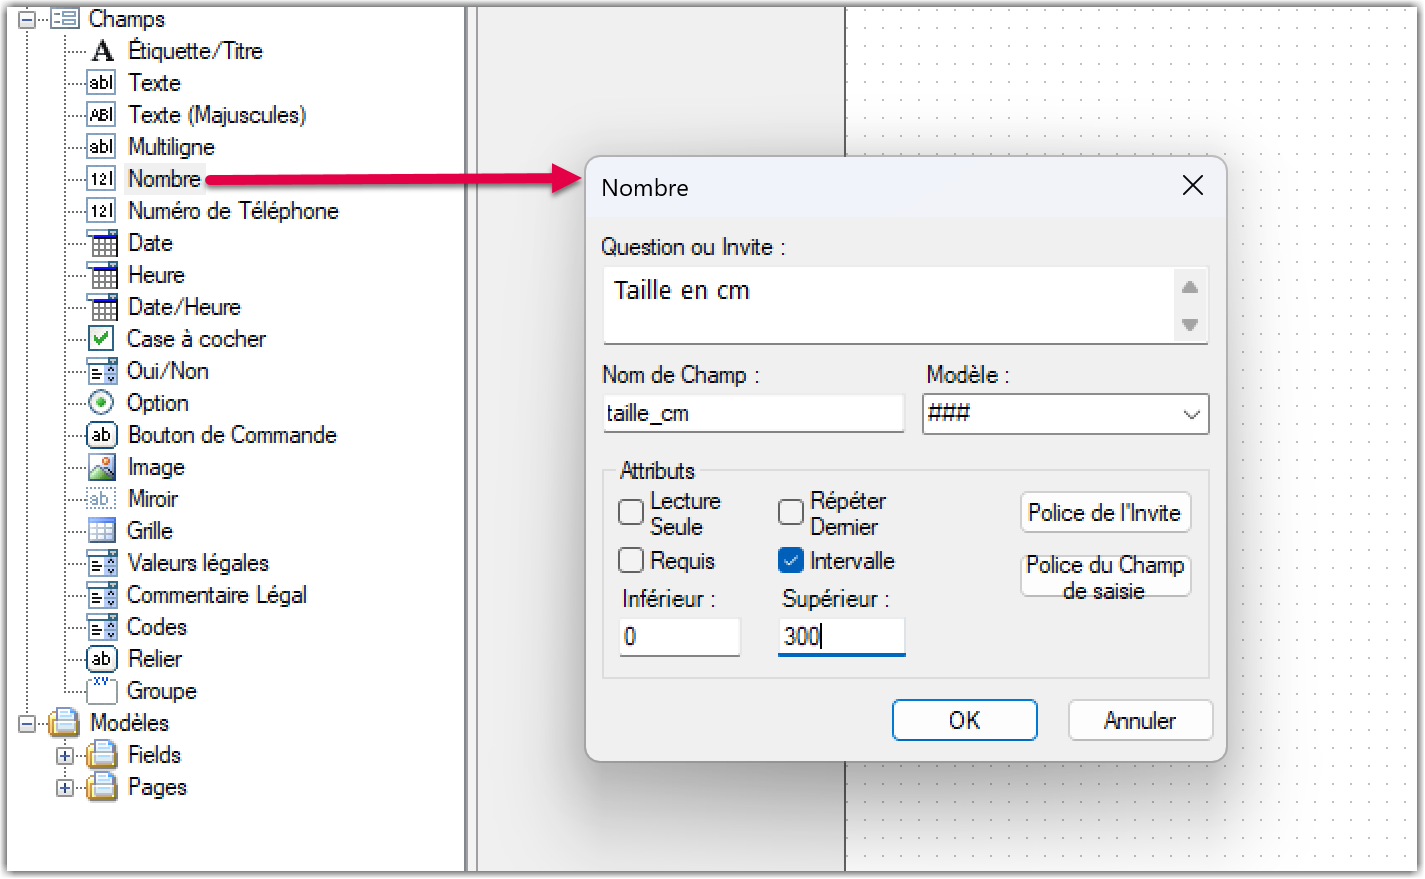
\includegraphics[width=\linewidth,height=0.4\textheight,keepaspectratio]{img/questionnaire/ajoutChampNombre}
	\caption{Ajouter un champ Nombre}
	\label{fig:ajoutchampnombre}
\end{figure}

\section{Ajouter un champ de type date ou heure}

Nous présentons ici l'ajout d'un champ de type Date ; la procédure est la même pour les champs de type Date/Heure et Heure. Nous créons ainsi les champs \var{date\_naissance} et \var{date\_enquete}.

\begin{enumerate}
	\item Double-cliquer sur \kw{Date}. Une fenêtre nommée Date s'ouvre ;
	\item Saisir la question dans la case prévue à cet effet ;
	\item Corriger le nom du champ si besoin ;
	\item Dans les attributs, cocher \kw{Requis} pour rendre le champ obligatoire, \kw{Lecture seule} si aucune modification ne doit être possible, ou \kw{Intervalle} pour définir une plage de dates acceptables. Modifier la police si besoin ;
	\item Valider par \kw{OK} pour créer le champ (\autoref{fig:ajoutchampdate}).
\end{enumerate}

Pour la date de naissance (\autoref{fig:ajoutchampdate}), nous avons coché \kw{Intervalle} avec pour bornes le 29/09/1900 et le 29/09/2023, date de création du formulaire : une date de naissance située dans le futur sera ainsi refusée.

\begin{figure}[H]
	\centering
	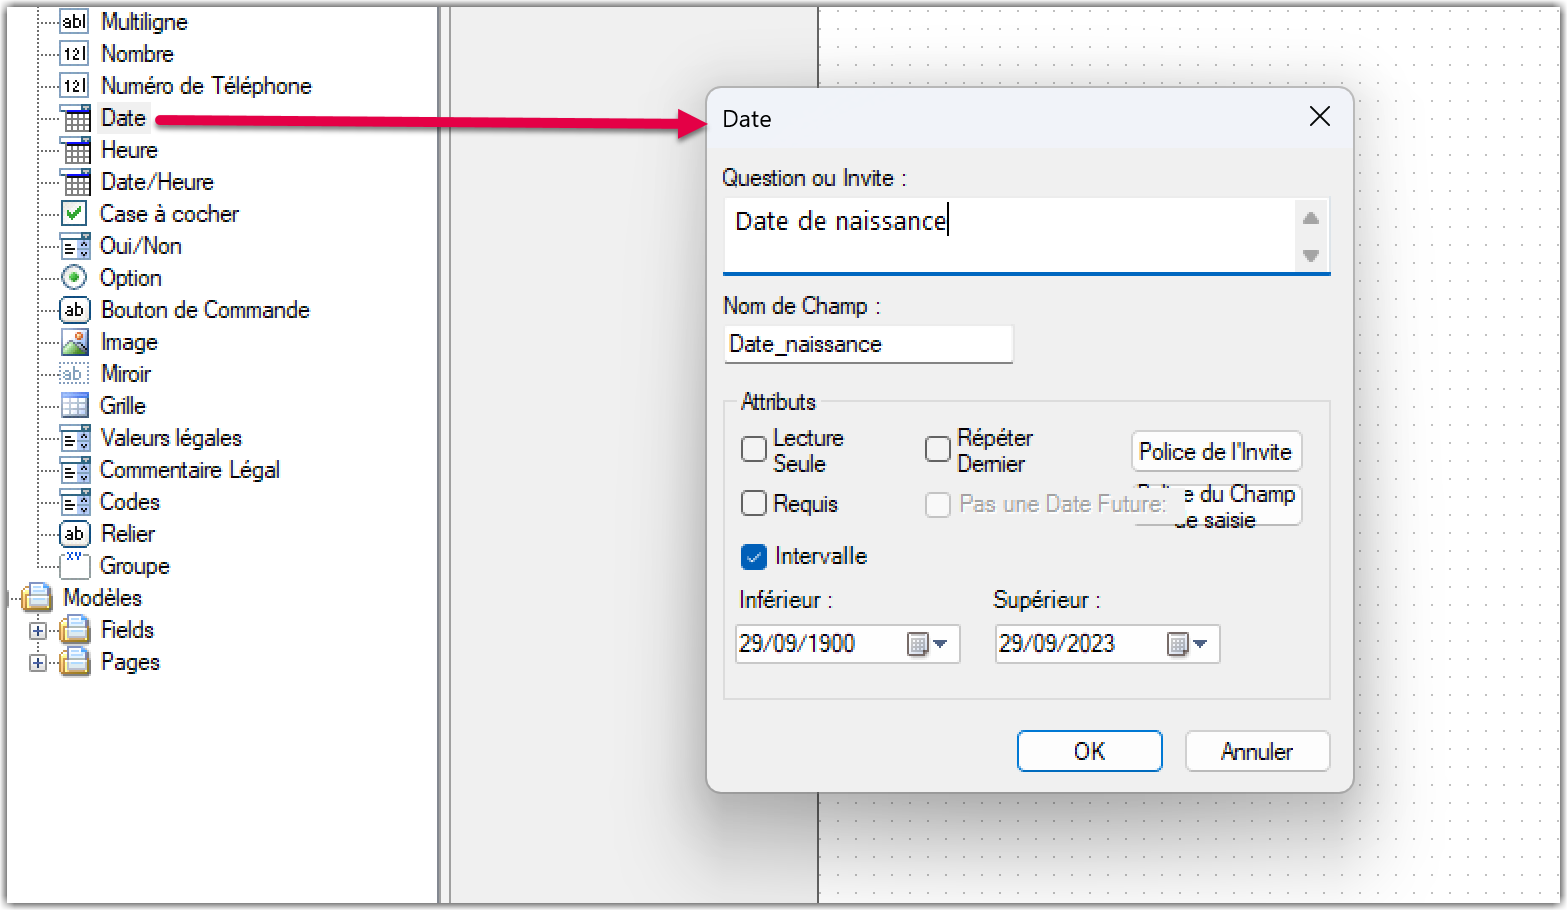
\includegraphics[width=\linewidth,height=0.4\textheight,keepaspectratio]{img/questionnaire/ajoutChampDate}
	\caption{Ajouter un champ de type Date ou Heure}
	\label{fig:ajoutchampdate}
\end{figure}

\section{Ajouter un champ de type Oui/Non}

Le champ Oui/Non est un champ de type booléen\footnote{Type informatique dont la valeur est soit vraie (\emph{True}), soit fausse (\emph{False}).} : il répond à une question par Oui ou Non. C'est ce type de champ que nous utilisons pour la question \og Êtes-vous vacciné(e) ? \fg{} (variable \var{vaccination}).

\begin{enumerate}
\item Double-cliquer sur \kw{Oui/Non}. Une fenêtre nommée Oui/Non s'ouvre ;
\item Saisir la question dans la case prévue à cet effet ;
\item Corriger le nom du champ si besoin ;
\item Dans les attributs, cocher \kw{Requis} pour rendre le champ obligatoire, \kw{Lecture seule} si aucune modification ne doit être possible, et modifier la police si besoin ;
\item Valider par \kw{OK} pour créer le champ (\autoref{fig:ajoutchampouinon}).
\end{enumerate}

\begin{figure}[H]
	\centering
	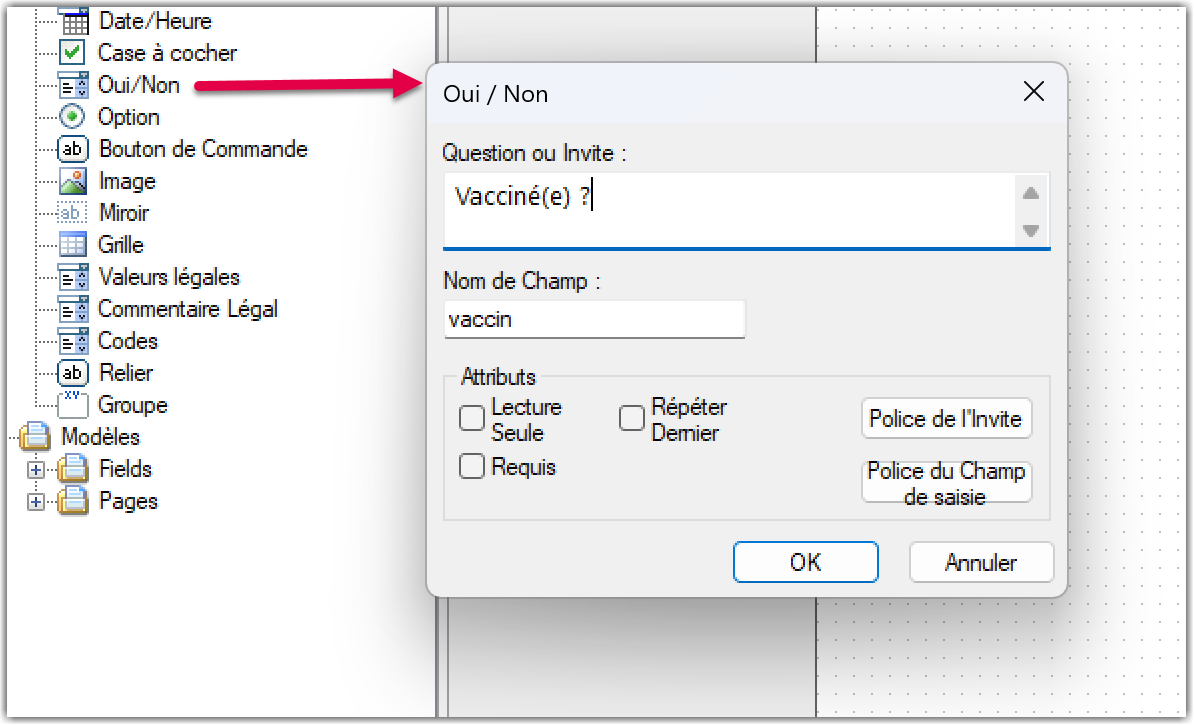
\includegraphics[width=\linewidth,height=0.4\textheight,keepaspectratio]{img/questionnaire/ajoutChampOuiNon}
	\caption{Ajouter un champ Oui/Non}
	\label{fig:ajoutchampouinon}
\end{figure}

\section{Ajouter un champ de type case à cocher}

Ce type de champ sert aux questions à choix multiples, c'est-à-dire aux questions qui admettent plusieurs réponses. Chaque réponse possible est une case à cocher distincte. Pour la question sur les symptômes, nous créons ainsi les cases \kw{Fièvre}, \kw{Céphalées}, \kw{Toux}, \kw{Mal de gorge}, \kw{Perte de l'odorat/du goût}, \kw{Fatigue}, \kw{Nausées/Vomissements} et \kw{Diarrhée}.

Double-cliquer sur \kw{Case à cocher} et saisir le libellé de la réponse, puis valider par \kw{OK}. S'il existe huit réponses possibles, vous répéterez l'opération huit fois. La \autoref{fig:ajoutcaseacocher} montre la création du champ \kw{Fièvre}.

\begin{figure}[H]
	\centering
	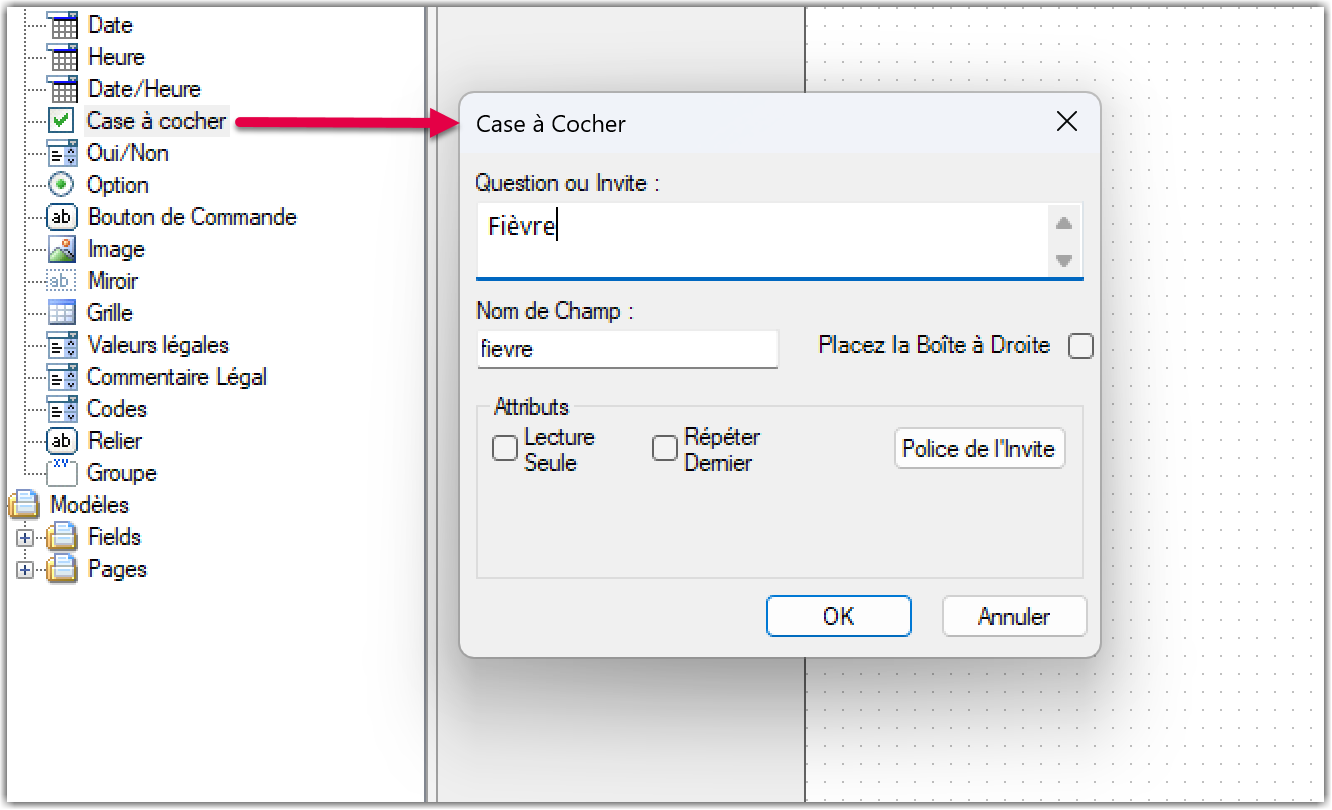
\includegraphics[width=\linewidth,height=0.4\textheight,keepaspectratio]{img/questionnaire/ajoutCaseAcocher}
	\caption{Créer un champ case à cocher}
	\label{fig:ajoutcaseacocher}
\end{figure}

Créées ainsi, les cases à cocher restent isolées les unes des autres. Nous allons donc les rassembler sous une bannière qui correspond à la question posée : c'est ce que l'on appelle la création d'un groupe (section suivante).

\section{Créer un groupe}
\label{creerGroupe}

Comme nous venons de le voir, l'option \kw{Groupe} permet de rassembler plusieurs champs sous une même bannière. Il peut s'agir des cases à cocher d'une question à choix multiples, mais aussi, par exemple, des champs nom, prénom, âge, sexe et profession du patient, regroupés sous l'intitulé \emph{Caractéristiques sociodémographiques}.

Pour grouper des champs :

\begin{enumerate}
	\item Sélectionner tous les champs du groupe\footnote{Pour sélectionner plusieurs champs, tracer un rectangle avec le bouton gauche de la souris maintenu enfoncé jusqu'à encadrer tous les champs.} ;
	\item Cliquer sur \kw{Insérer} dans la barre d'outils, puis sur \kw{Groupe} (\autoref{fig:ajoutgroupe}) ;
	\item Saisir l'intitulé du groupe dans \kw{Question ou Invite}, ici \question{Symptômes}, et vérifier le nom du champ, ici \var{symptomes} ;
	\item Changer la police si besoin ;
	\item Valider la création du groupe en cliquant sur \kw{OK}.
\end{enumerate}

\begin{figure}[H]
	\centering
	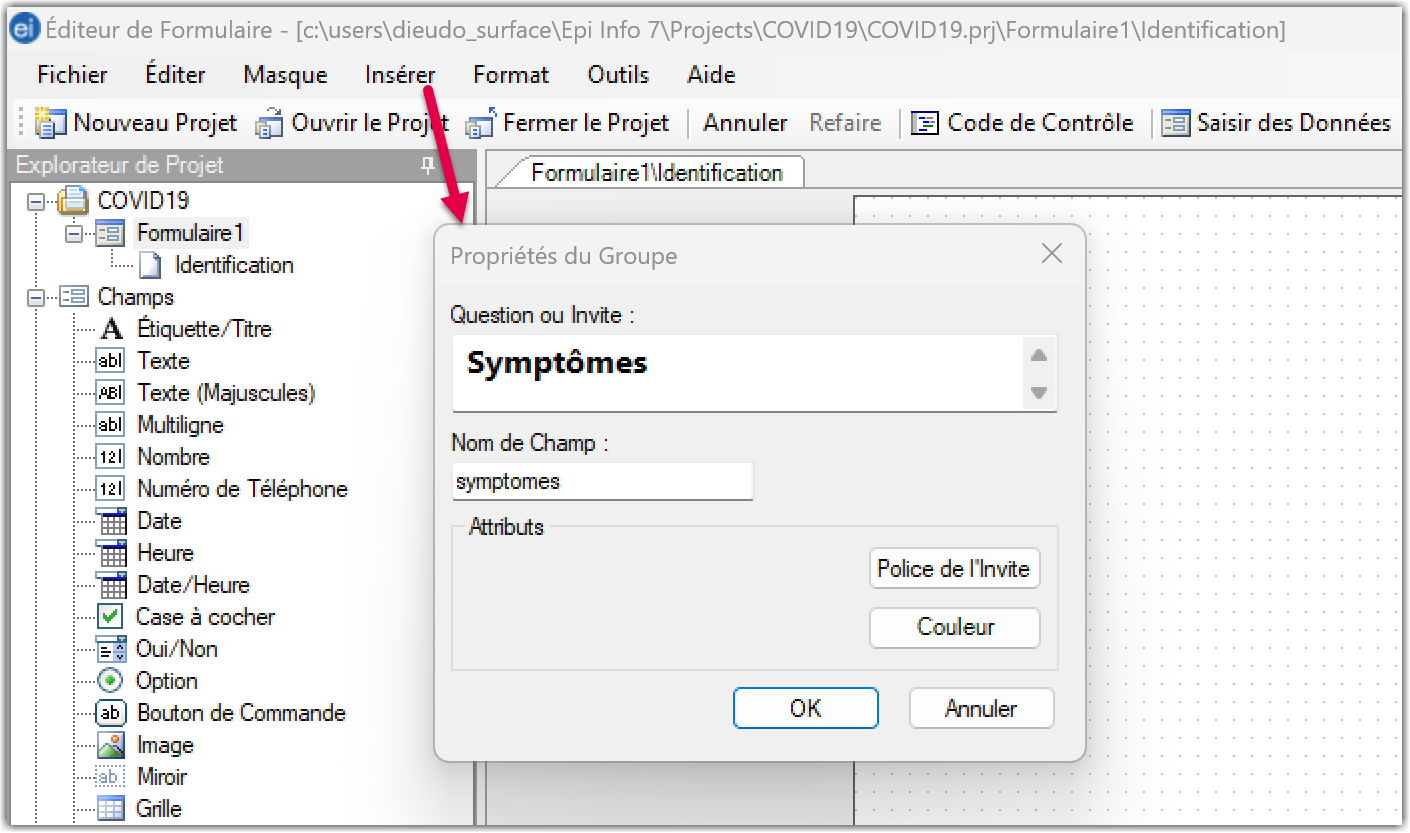
\includegraphics[width=\linewidth,height=0.4\textheight,keepaspectratio]{img/questionnaire/ajoutGroupe}
	\caption{Créer un groupe}
	\label{fig:ajoutgroupe}
\end{figure}

\begin{mybox}[colbacktitle=IMPORTANT]{\faExclamationCircle{} IMPORTANT}
Pour créer un groupe, commencez toujours par créer les champs qui le composent (les cases à cocher d'une question à choix multiples, par exemple). Pour supprimer un groupe, faites un clic droit sur le groupe puis choisissez \kw{Supprimer}.
\end{mybox}

%%%%%%%%%%%%%%%%%%% Créer un champ Valeurs légales %%%%%%%%%%%%%%%%%%%%%
\section{Ajouter un champ de type valeurs légales}
\label{sec:valeursLegales}

Le champ \kw{Valeurs légales} présente les réponses possibles à une question sous la forme d'une liste déroulante. C'est l'un des moyens les plus simples d'assurer une saisie exacte. Il est très utile lorsque la réponse ne peut prendre qu'un nombre limité de valeurs (\autoref{fig:ajoutvaleurslegales}).

\begin{enumerate}
	\item Double-cliquer sur \kw{Valeurs légales}. Une fenêtre nommée Valeurs légales s'ouvre ;
	\item Saisir la question dans le champ \kw{Question ou Invite} et changer la police si besoin. Notre question est \question{Pourquoi n'êtes-vous pas vacciné(e) ?} ;
	\item Appuyer sur la touche de tabulation et corriger le nom du champ, ici \var{pourquoi\_pas\_vaccine} ;
	\item Dans la partie \kw{Source de données}, cliquer sur le petit carré contenant trois points ;
	\item Dans la fenêtre \kw{Définir le code / les liens légaux} qui s'ouvre, cliquer en bas sur \kw{Créer un nouveau} ;
	\item Saisir les réponses possibles dans la zone qui apparaît, ici \kw{Je ne vois pas la nécessité de me faire vacciner}, \kw{Je ne fais pas confiance au vaccin} et \kw{Autre réponse}. Par défaut, les réponses sont triées par ordre alphabétique ; cocher la case \kw{Ne pas trier}, en bas à gauche, pour conserver l'ordre de saisie ;
	\item Valider le tout par \kw{OK}.
\end{enumerate}

Pour permettre de préciser une \og autre réponse \fg{}, nous créons aussi un champ texte nommé \var{autre\_reponse\_non\_vaccination}, avec pour invite \question{Autre réponse liée à la non-vaccination}. Nous l'utiliserons au chapitre~\ref{codeValidation}.

\begin{figure}[H]
	\centering
	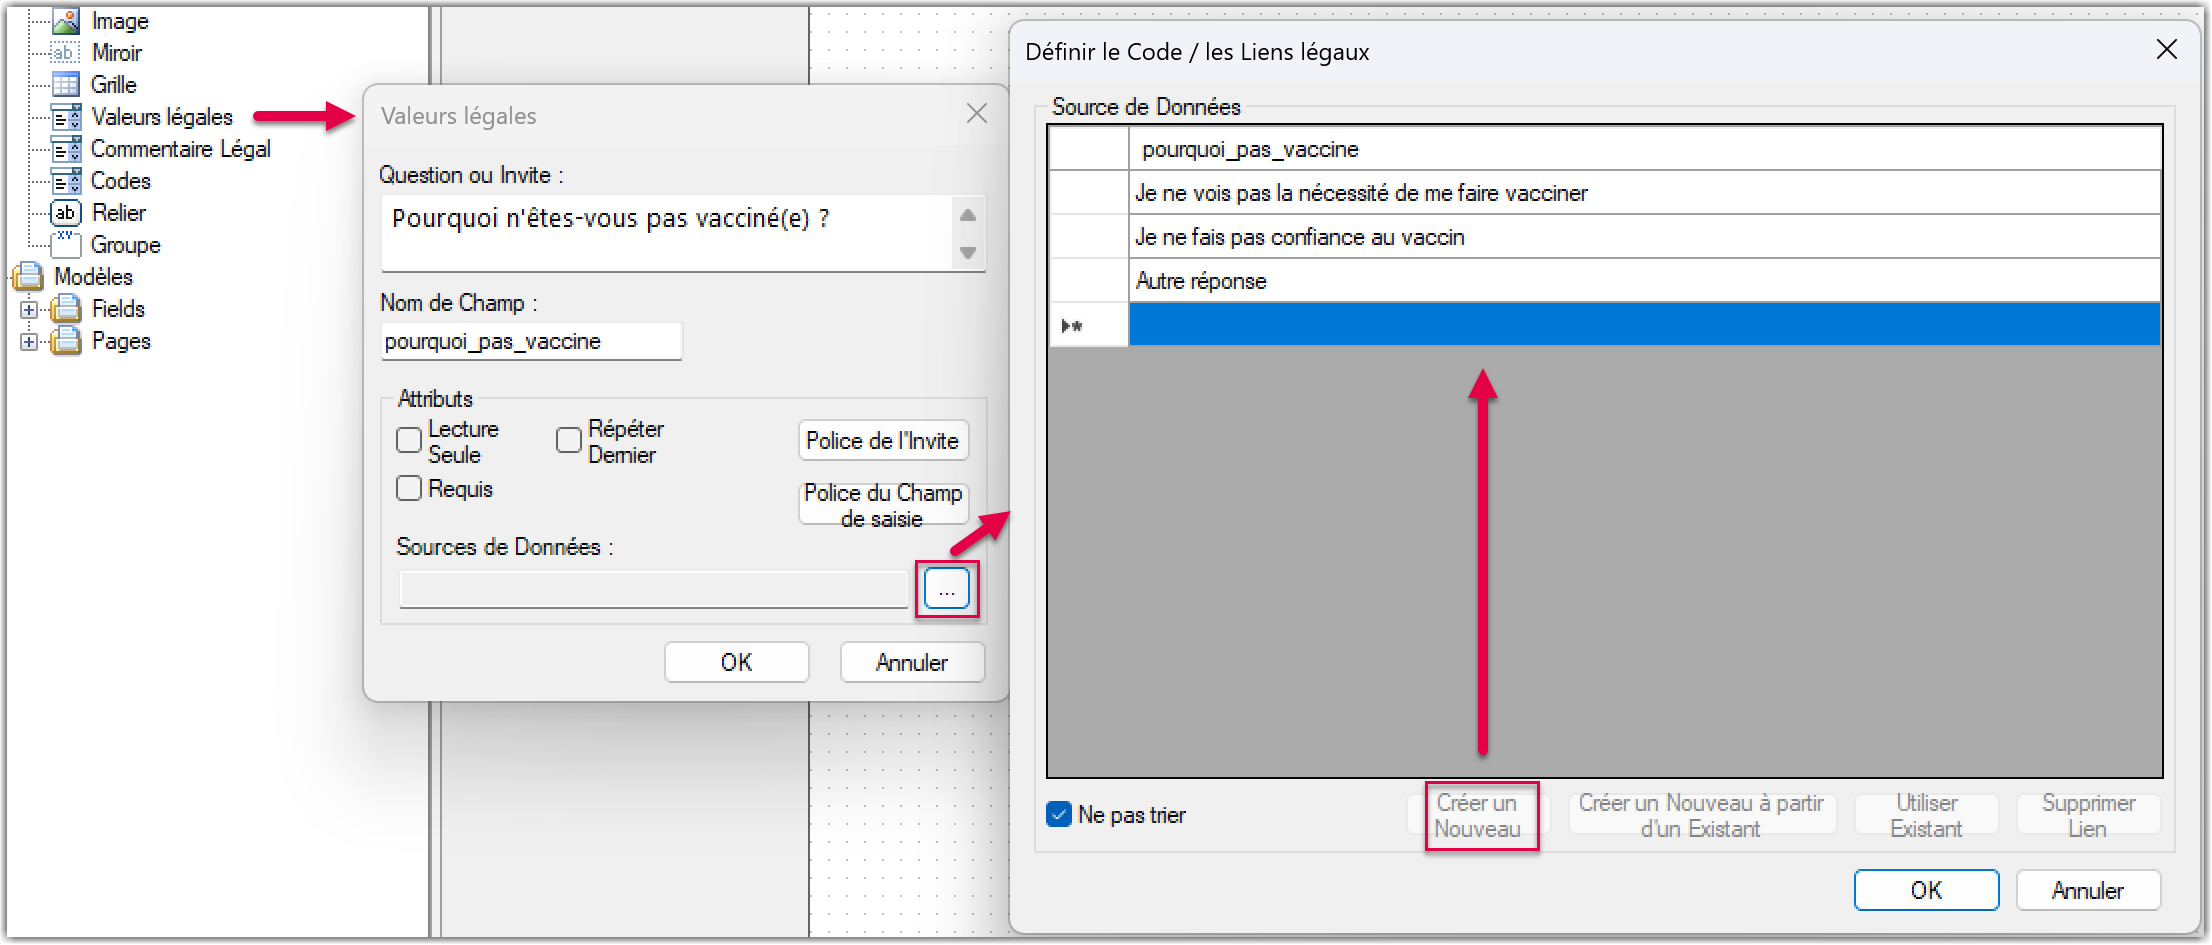
\includegraphics[width=\linewidth,height=0.4\textheight,keepaspectratio]{img/questionnaire/ajoutValeursLegales}
	\caption{Ajouter un champ Valeurs légales}
	\label{fig:ajoutvaleurslegales}
\end{figure}

%%%%%%%%%%%%%%%%%%% Créer un champ de type Option %%%%%%%%%%%%%%%%%%%%%
\section{Ajouter un champ de type option}
\label{sec:option}

Le champ \kw{Option} affiche des boutons radio et n'autorise qu'une seule réponse. Nous vous montrons comment l'utiliser, mais c'est un type de champ qu'il vaut mieux éviter (voir l'avertissement ci-dessous). Par exemple, la question précédente, \question{Pourquoi n'êtes-vous pas vacciné(e) ?}, aurait pu être posée avec un champ Option plutôt qu'avec un champ Valeurs légales (section~\ref{sec:valeursLegales}, page~\pageref{sec:valeursLegales}).

C'est ce que montre la \autoref{fig:ajoutchampoption}, page~\pageref{fig:ajoutchampoption}, avec les trois réponses possibles :

\begin{enumerate}
	\item Double-cliquer sur \kw{Option}. Une fenêtre nommée Option s'ouvre ;
	\item Saisir la question dans le champ \kw{Question ou Invite}, ici \question{Pourquoi n'êtes-vous pas vacciné(e) ?}, et changer la police si besoin ;
	\item Appuyer sur la touche de tabulation et corriger le nom du champ si besoin, ici \var{pourquoi\_pas\_vaccine} ;
	\item Choisir d'afficher les options verticalement (choix par défaut) ou horizontalement ;
	\item Choisir de commencer la liste des options à gauche (choix par défaut) ou à droite ;
	\item Dans les attributs, au niveau de \kw{Nombre de choix}, choisir avec les flèches le nombre de réponses possibles, ici 3 ;
	\item Dans la partie \kw{Définition d'options}, saisir les trois réponses, puis valider par \kw{OK}.
\end{enumerate}

\begin{figure}[H]
	\centering
	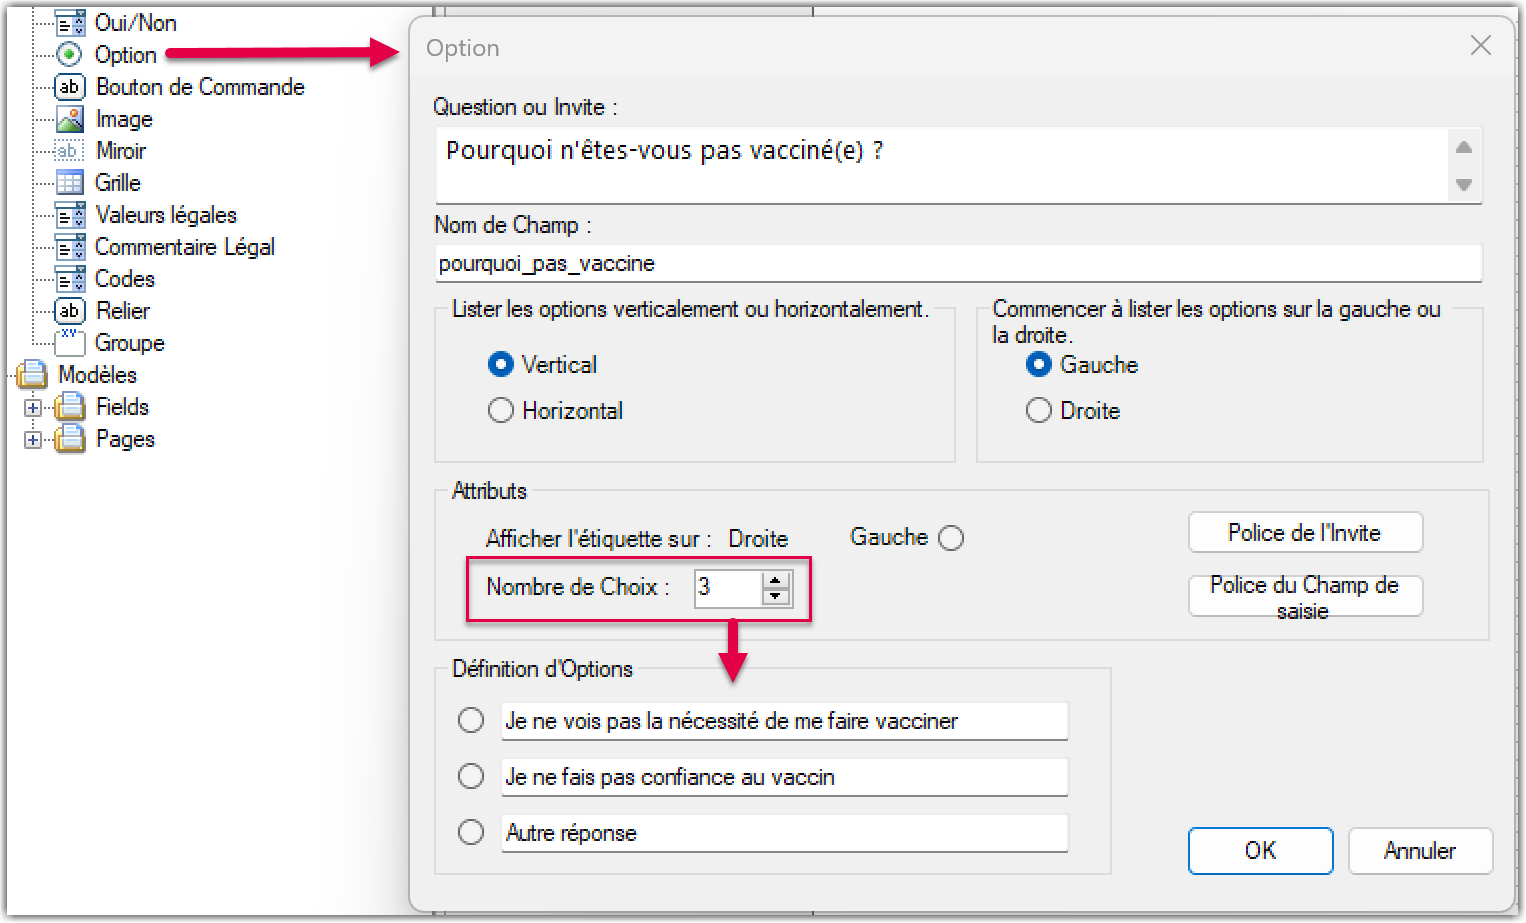
\includegraphics[width=\linewidth,height=0.4\textheight,keepaspectratio]{img/questionnaire/ajoutChampOption}
	\caption{Ajouter un champ Option}
	\label{fig:ajoutchampoption}
\end{figure}

\begin{mybox}[colbacktitle=CAUTION]{\faFire{} AVERTISSEMENT}
	Utiliser un champ Option peut avoir des conséquences graves sur vos données.
	En effet, un champ Option n'enregistre pas le libellé de la réponse dans la base de données, mais sa position dans la liste. Si la question sur la vaccination était posée avec un champ Option, \kw{Je ne vois pas la nécessité de me faire vacciner} serait enregistré sous la valeur 0, \kw{Je ne fais pas confiance au vaccin} sous la valeur 1, etc.
	Si, pour une raison ou une autre, vous modifiez ensuite l'ordre des réponses de sorte que \kw{Autre réponse} passe en première position, cette réponse prendra la valeur 0\ldots{} mais les données déjà enregistrées ne seront pas mises à jour.
	Il est donc recommandé d'utiliser les listes déroulantes (Valeurs légales, Commentaire légal, etc.) plutôt que les champs Option.
\end{mybox}

%%%%%%%%%%%%%%%%%%% Créer un champ commentaire légal %%%%%%%%%%%%%%%%%%%%%
\section{Ajouter un champ de type commentaire légal}
\label{sec:commentaireLegal}

Comme le champ Valeurs légales, le champ \kw{Commentaire légal} présente les réponses possibles sous la forme d'une liste déroulante. La différence est que chaque réponse est précédée d'un code, alphabétique ou numérique ; le code et la réponse sont reliés par un trait d'union (\textcolor{IMPORTANT}{$-$}). C'est le code qui est enregistré dans la base de données, ce qui facilite l'analyse. Prenons l'exemple de la situation matrimoniale (\autoref{fig:ajoutcommentairelegal}) :

\begin{enumerate}
	\item Double-cliquer sur \kw{Commentaire légal}. Une fenêtre nommée Commentaire légal s'ouvre ;
	\item Saisir la question dans le champ \kw{Question ou Invite} et changer la police si besoin ;
	\item Appuyer sur la touche de tabulation et corriger le nom du champ si besoin, par exemple \var{situation\_matrimoniale} ;
	\item Dans la partie \kw{Source de données}, cliquer sur le petit carré contenant trois points, situé en bas à droite ;
	\item Dans la fenêtre \kw{Définir le code / les liens légaux} qui s'ouvre, cliquer en bas sur \kw{Créer un nouveau} ;
	\item Saisir les réponses, chacune précédée de son code, dans la zone qui apparaît. Dans notre cas : \kw{C-Célibataire}, \kw{M-Marié(e)} et \kw{D-Divorcé(e)} ;
	\item Valider le tout par \kw{OK}.
\end{enumerate}

\begin{figure}[H]
	\centering
	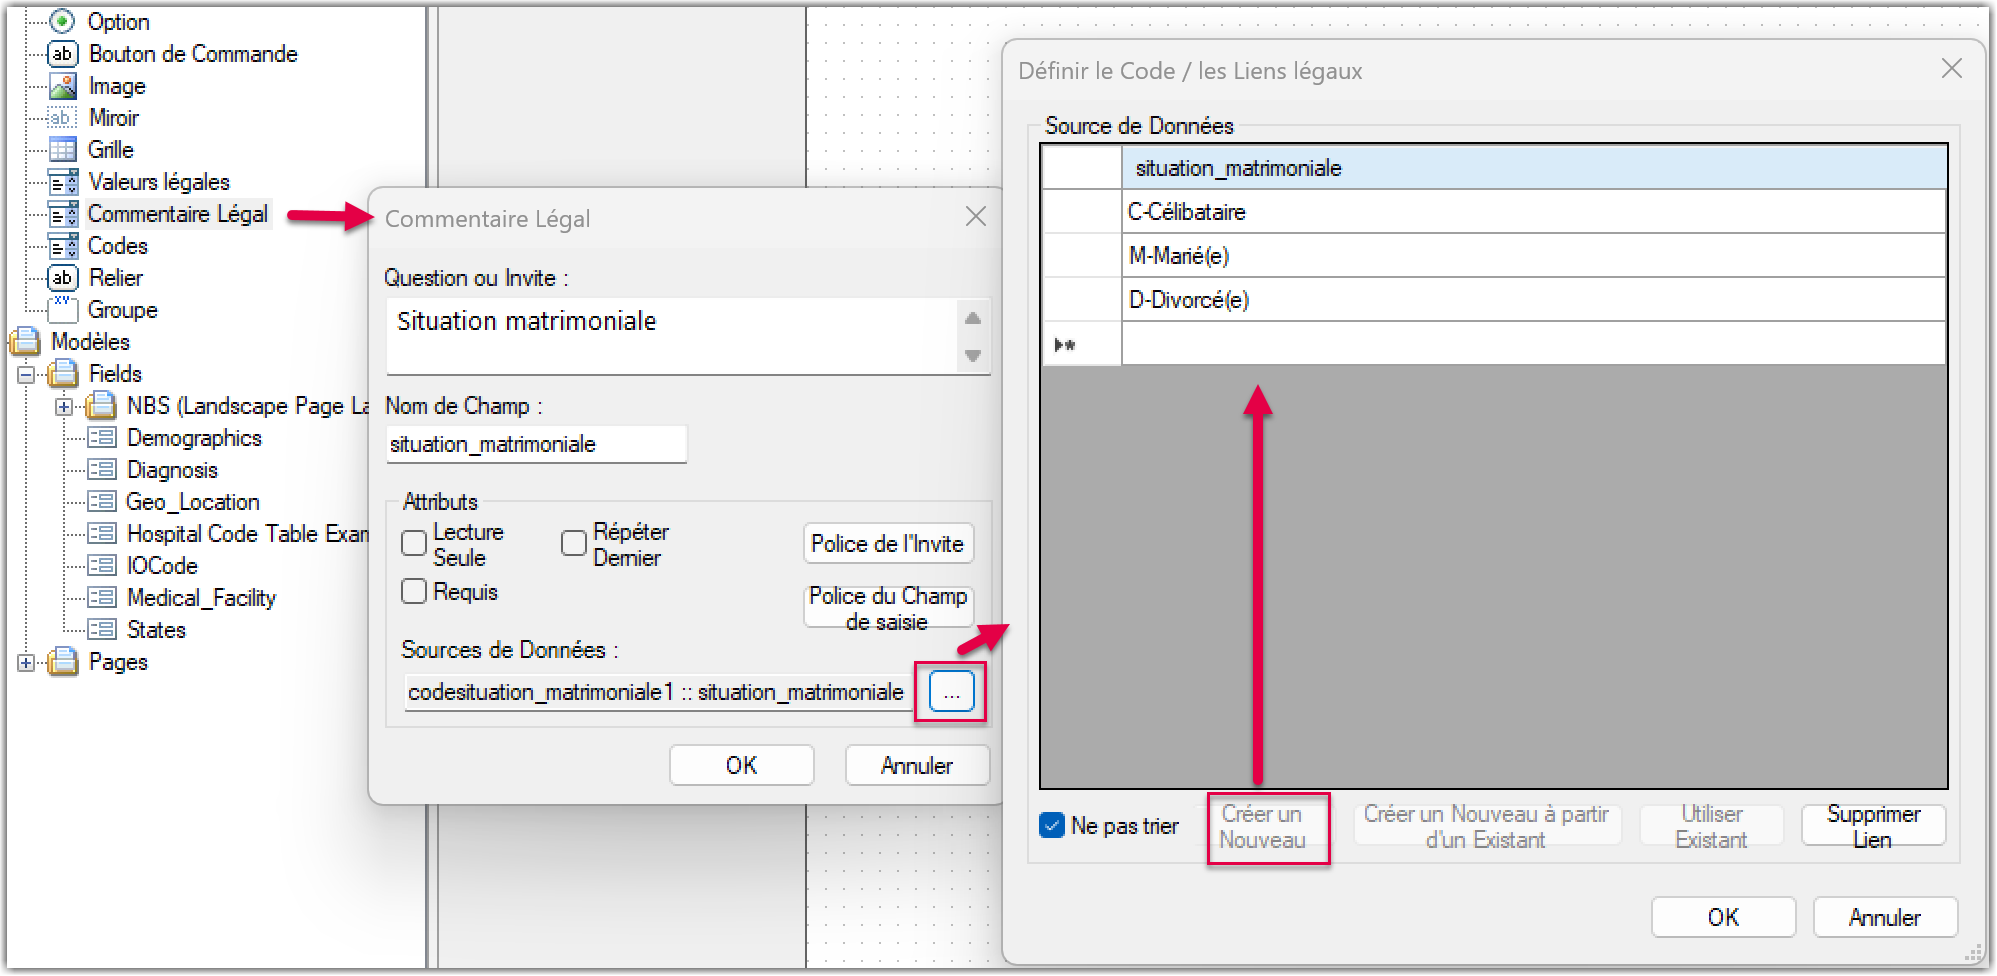
\includegraphics[width=\linewidth,height=0.4\textheight,keepaspectratio]{img/questionnaire/ajoutCommentaireLegal}
	\caption{Ajouter un champ Commentaire légal}
	\label{fig:ajoutcommentairelegal}
\end{figure}

\begin{mybox}[colbacktitle=NOTE]{\faInfoCircle{} À RETENIR}
	Il est également possible de reproduire cet exemple avec un champ Valeurs légales (voir la section~\ref{sec:valeursLegales}, \nameref{sec:valeursLegales}, page~\pageref{sec:valeursLegales}), mais sans les codes.
\end{mybox}

\section{Ajouter un champ de géolocalisation}

Il est possible d'ajouter un champ de géolocalisation dans Epi Info. Pour cela :

\begin{itemize}
\item aller dans \kw{Modèles}, en bas de l'explorateur de projets (la barre latérale gauche) ;
\item ouvrir le dossier \kw{Fields} ;
\item faire un glisser-déposer de \kw{Geo\_Location} sur le canevas (\autoref{fig:geolocalisation}).
\end{itemize}

Ce modèle ajoute au formulaire les champs nécessaires pour enregistrer la latitude et la longitude du lieu de l'enquête.

\begin{figure}[H]
	\centering
	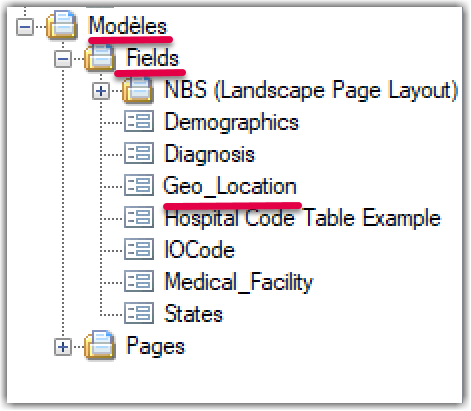
\includegraphics[width=0.5\linewidth]{img/questionnaire/geolocalisation}
	\caption{Ajouter un champ de géolocalisation}
	\label{fig:geolocalisation}
\end{figure}

\section{Les attributs de champ}

Vous avez sans doute remarqué que la fenêtre de définition d'un champ numérique diffère de celle d'un champ texte. Par exemple, le champ texte ne propose ni intervalle ni modèle. Chaque type de champ dispose en effet de ses propres options pour personnaliser son apparence et son comportement.
Parmi les attributs les plus courants figurent :

\begin{itemize}
	\item \kw{Intervalle} : permet de fixer une valeur minimale et une valeur maximale pour le champ. Toute valeur en dehors de ces bornes est refusée ;
	\item \kw{Requis} : un champ obligatoire doit être rempli avant que l'enregistrement puisse être sauvegardé ;
	\item \kw{Répéter le dernier} : le champ est automatiquement rempli avec la valeur de l'enregistrement précédent ;
	\item \kw{Lecture seule} : le champ ne peut pas être modifié par l'utilisateur. Cet attribut sert surtout aux champs calculés par le code de contrôle, comme l'âge ou l'IMC.
\end{itemize}

\section{L'outil dictionnaire des données}

Le dictionnaire des données est un résumé des champs créés. Il indique notamment, pour chaque champ, le numéro de la page, l'invite, le nom du champ, son type, sa mise en forme éventuelle et toute autre information qui lui est propre. Il est essentiel de relire le dictionnaire des données avant de commencer la collecte : cela permet de repérer les noms de champs mal choisis et de vérifier que chaque champ a le bon type et le bon format.

Pour afficher le dictionnaire, cliquer sur \kw{Outils} dans la barre d'outils, puis sur \kw{Dictionnaire des données}. Le dictionnaire peut être trié en cliquant sur le titre de chaque colonne. Il peut aussi être affiché dans un navigateur web et imprimé avec la commande d'impression du navigateur ou le raccourci clavier \kw{Ctrl + P}.

\section{Ajouter, renommer ou supprimer une page}
\label{ajouterPage}

Un formulaire peut contenir plusieurs pages. Notre formulaire en compte deux : la page \kw{Identification} et la page \kw{Signes cliniques}.

Pour ajouter une page, faire un clic droit sur le nom du formulaire dans l'explorateur de projets et cliquer sur \kw{Ajouter une page} (\autoref{fig:ajouterpage}). Pour supprimer ou renommer une page, faire un clic droit sur la page concernée puis choisir \kw{Supprimer} ou \kw{Renommer}.

\begin{figure}[H]
	\centering
	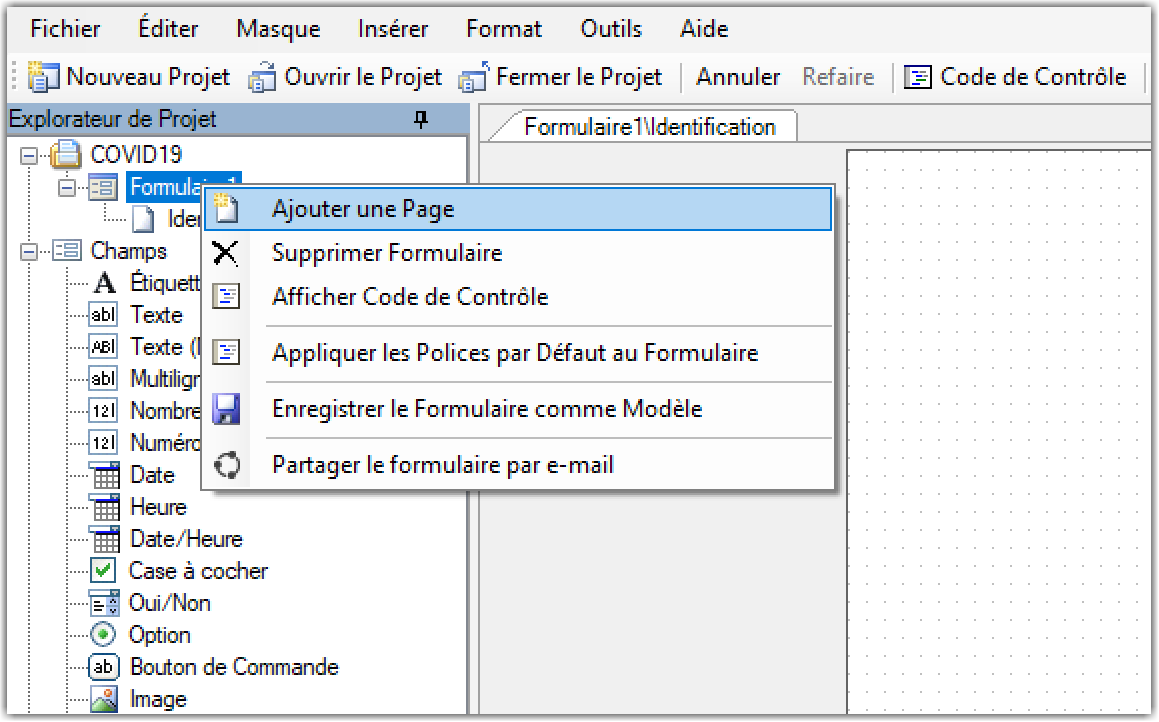
\includegraphics[width=\linewidth,height=0.4\textheight,keepaspectratio]{img/questionnaire/ajouterPage}
	\caption{Ajouter une page au formulaire}
	\label{fig:ajouterpage}
\end{figure}

\section{Changer l'ordre de tabulation}

Notre formulaire se présente comme sur la \autoref{fig:formulairepage1}, page~\pageref{fig:formulairepage1}, et la \autoref{fig:formulairepage2}, page~\pageref{fig:formulairepage2}.

\begin{figure}[H]
	\centering
	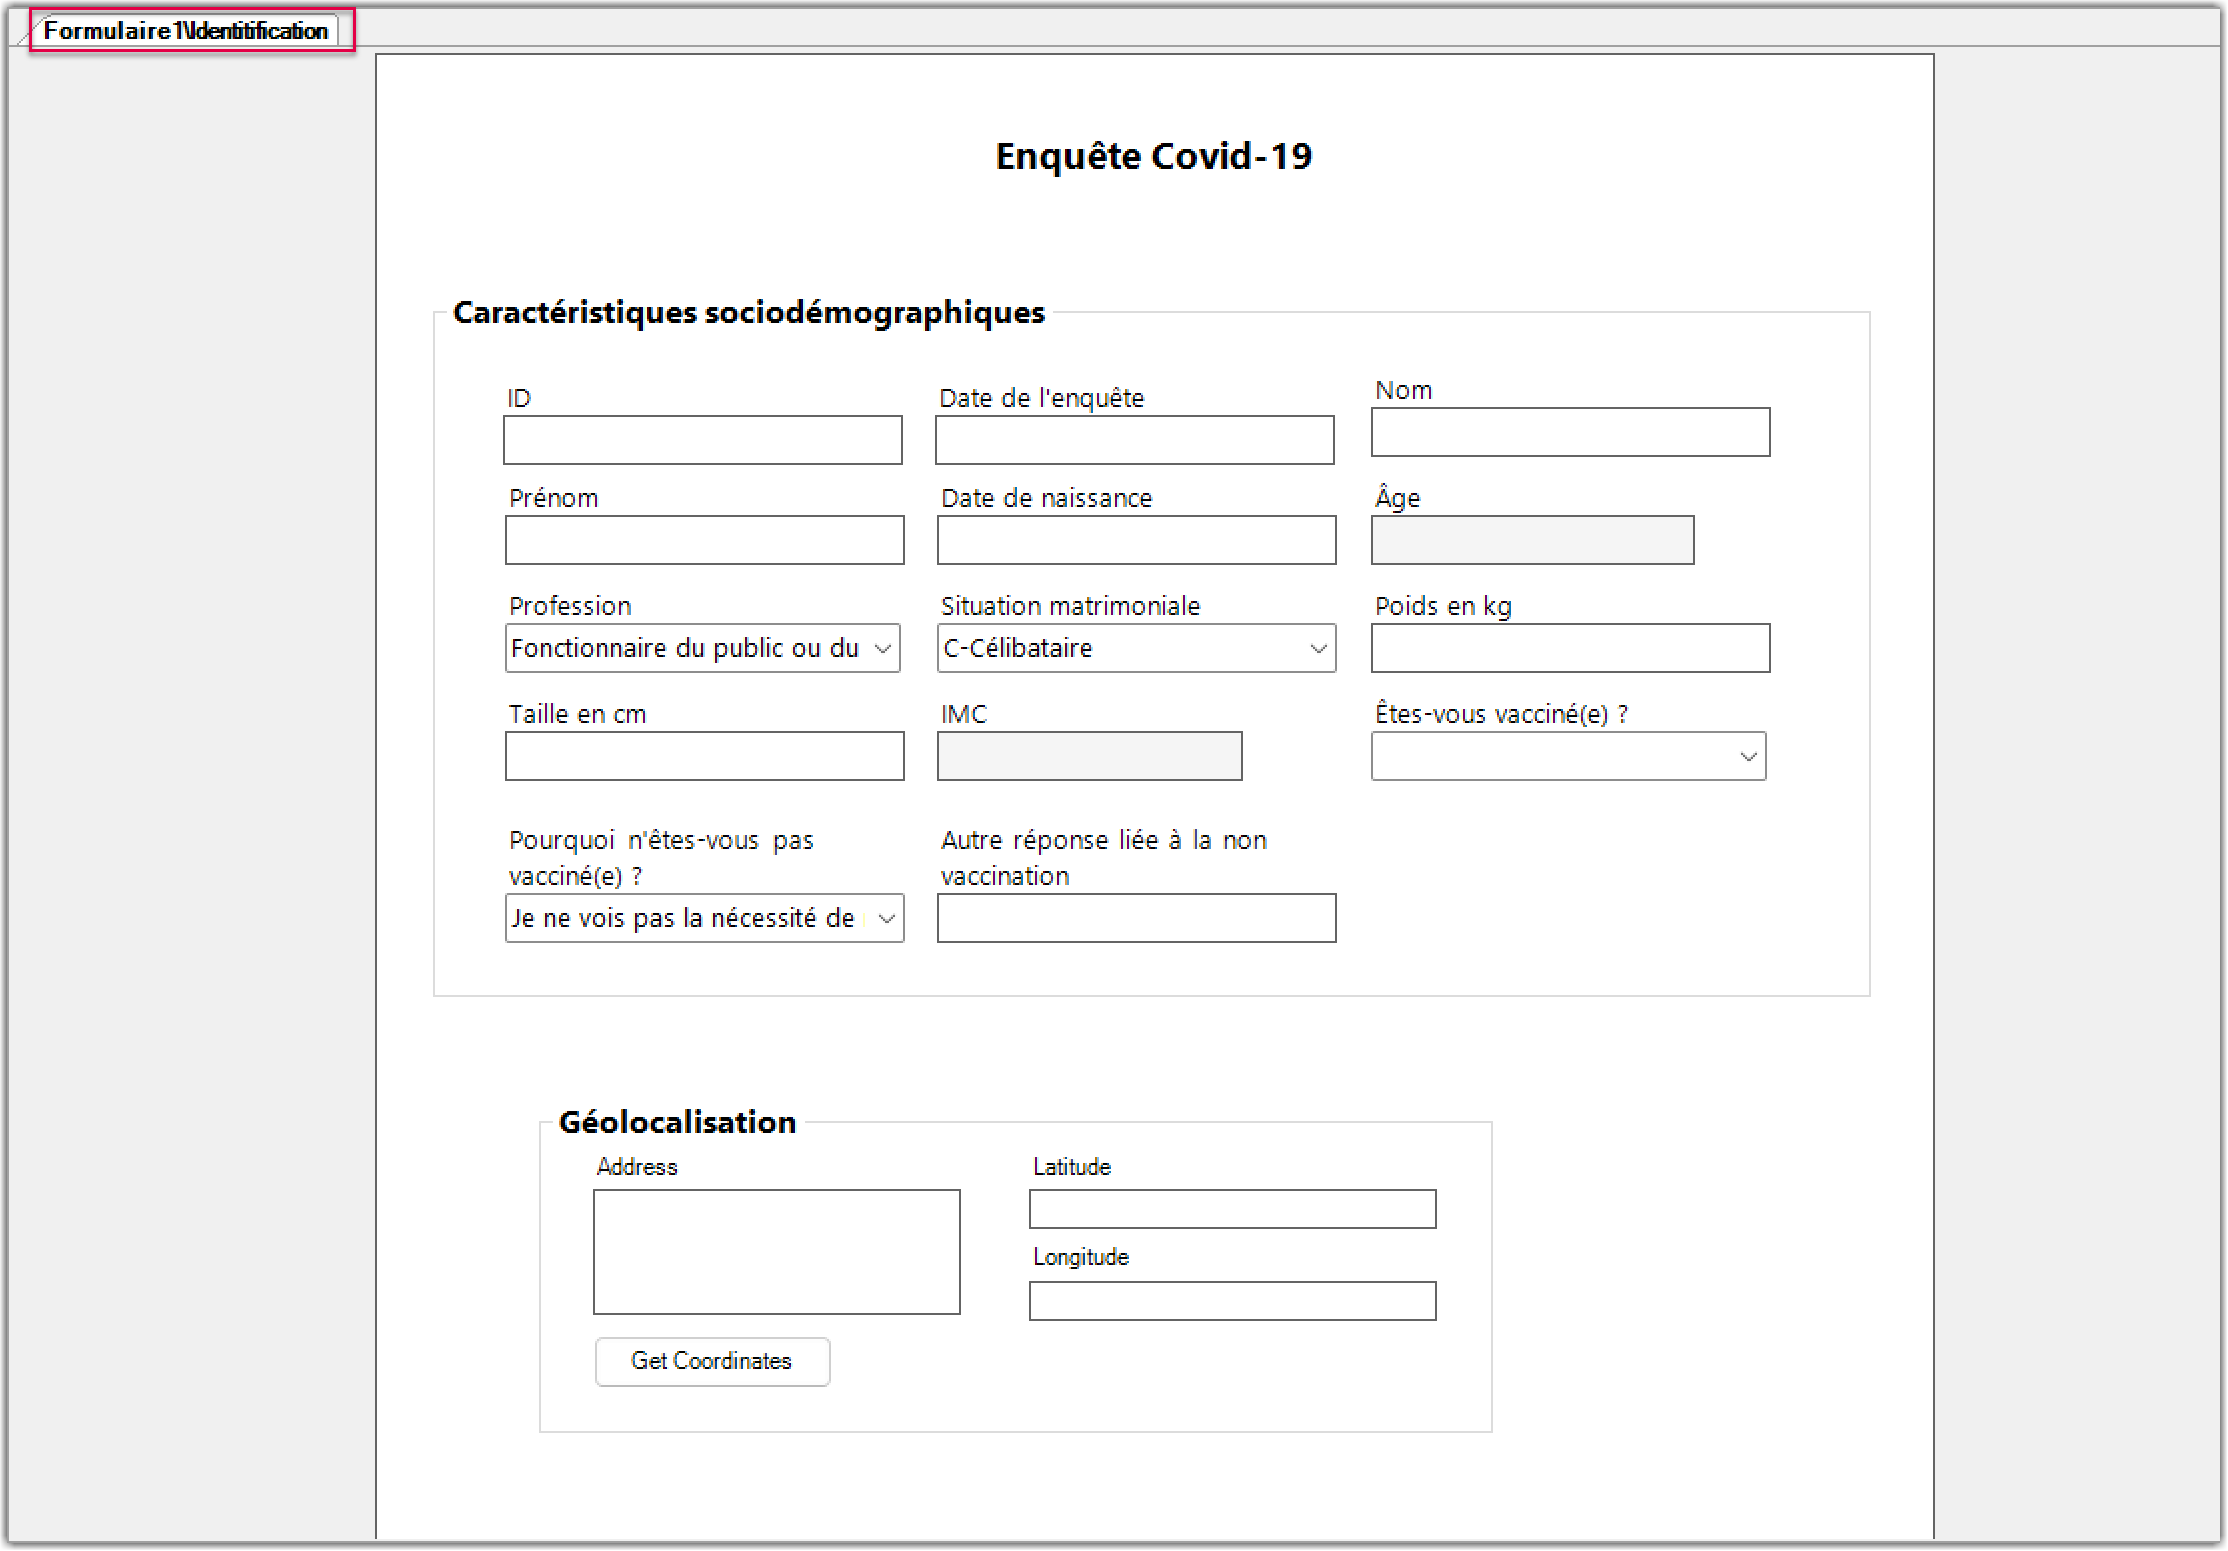
\includegraphics[width=\linewidth,height=0.4\textheight,keepaspectratio]{img/questionnaire/formulairePage1}
	\caption{Page Identification de notre formulaire}
	\label{fig:formulairepage1}
\end{figure}

\begin{figure}[H]
	\centering
	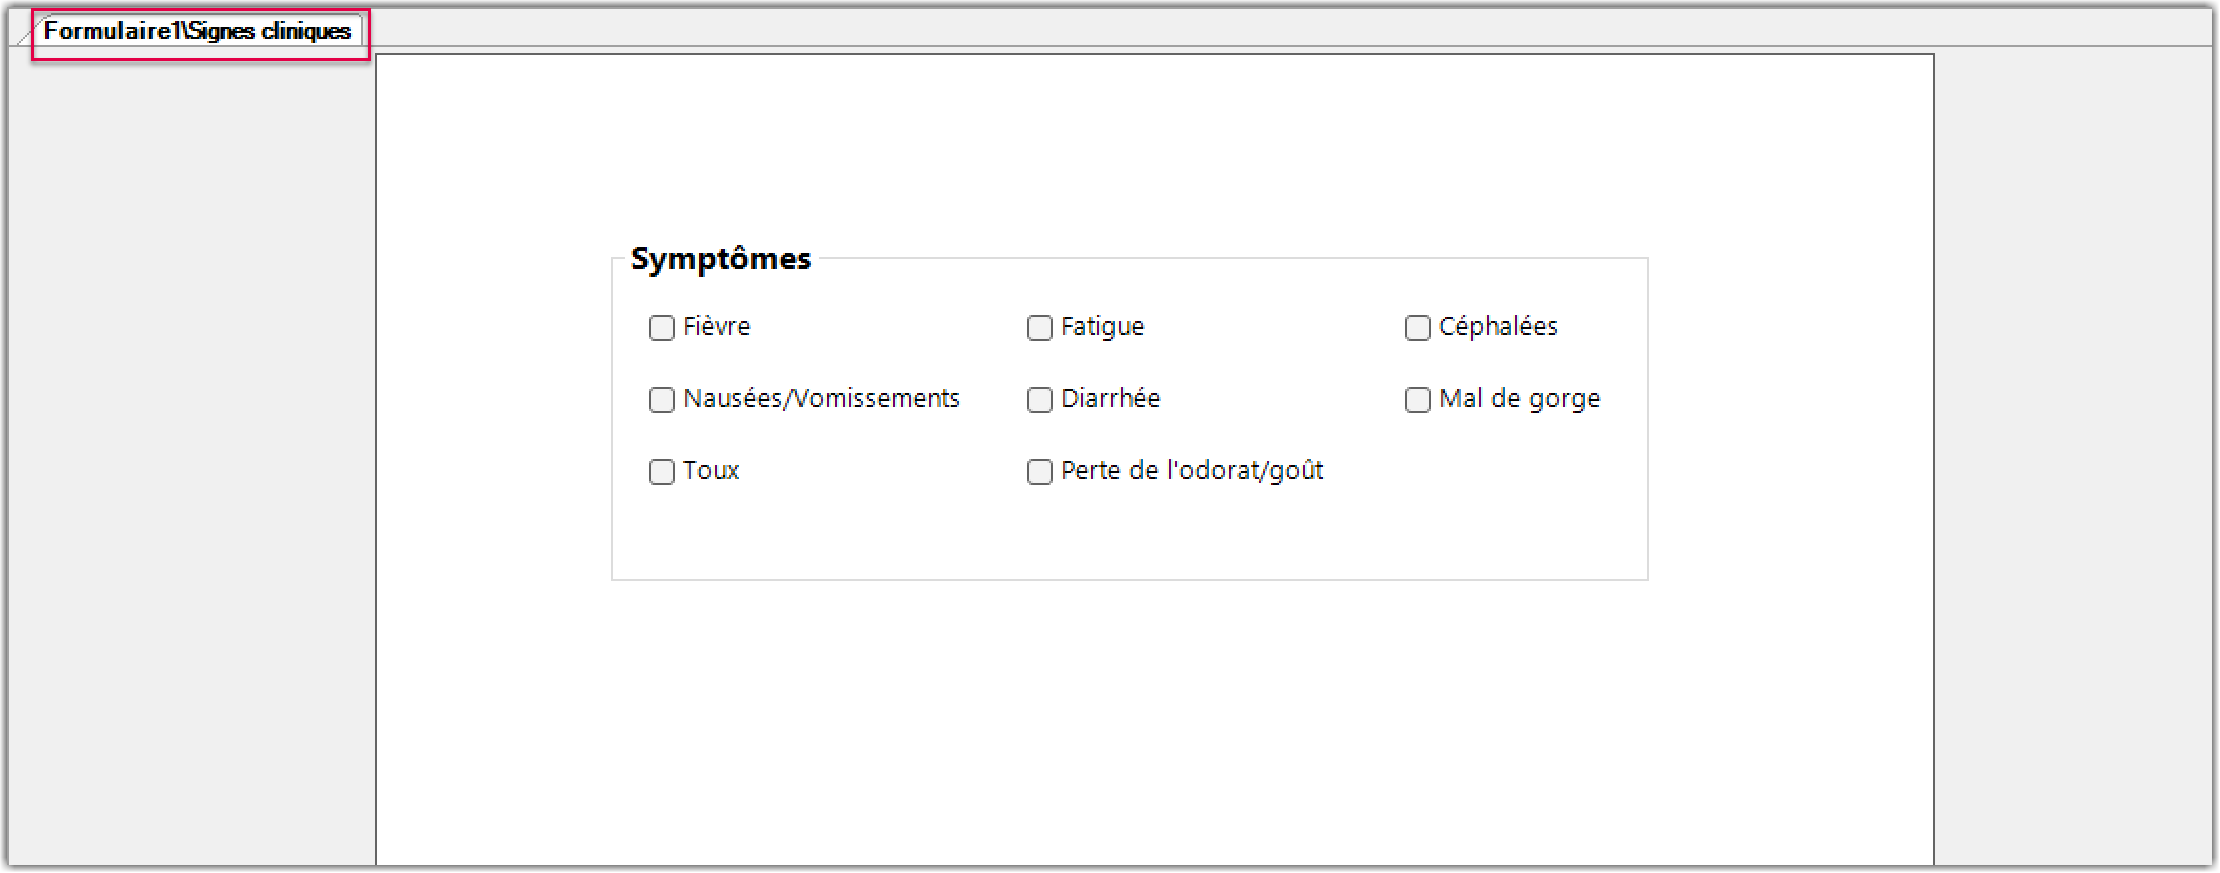
\includegraphics[width=\linewidth,height=0.4\textheight,keepaspectratio]{img/questionnaire/formulairePage2}
	\caption{Page Signes cliniques de notre formulaire}
	\label{fig:formulairepage2}
\end{figure}

L'ordre de tabulation est l'ordre dans lequel le curseur passe d'un champ à l'autre lorsque l'on appuie sur la touche Tabulation pendant la saisie. Il est fixé par défaut selon l'ordre de création des champs. Après réorganisation du formulaire sur le canevas, cet ordre ne correspond donc souvent plus à la disposition des questions.

Affichons d'abord l'ordre de tabulation actuel : faire un clic droit sur le canevas, aller dans \kw{Onglets} puis cliquer sur \kw{Montrer l'ordre des tabulations} (\autoref{fig:afficherordretabulation}). La \autoref{fig:ordretabulation} montre l'ordre de tabulation de notre formulaire. Le vôtre peut être différent.

\begin{figure}[H]
	\centering
	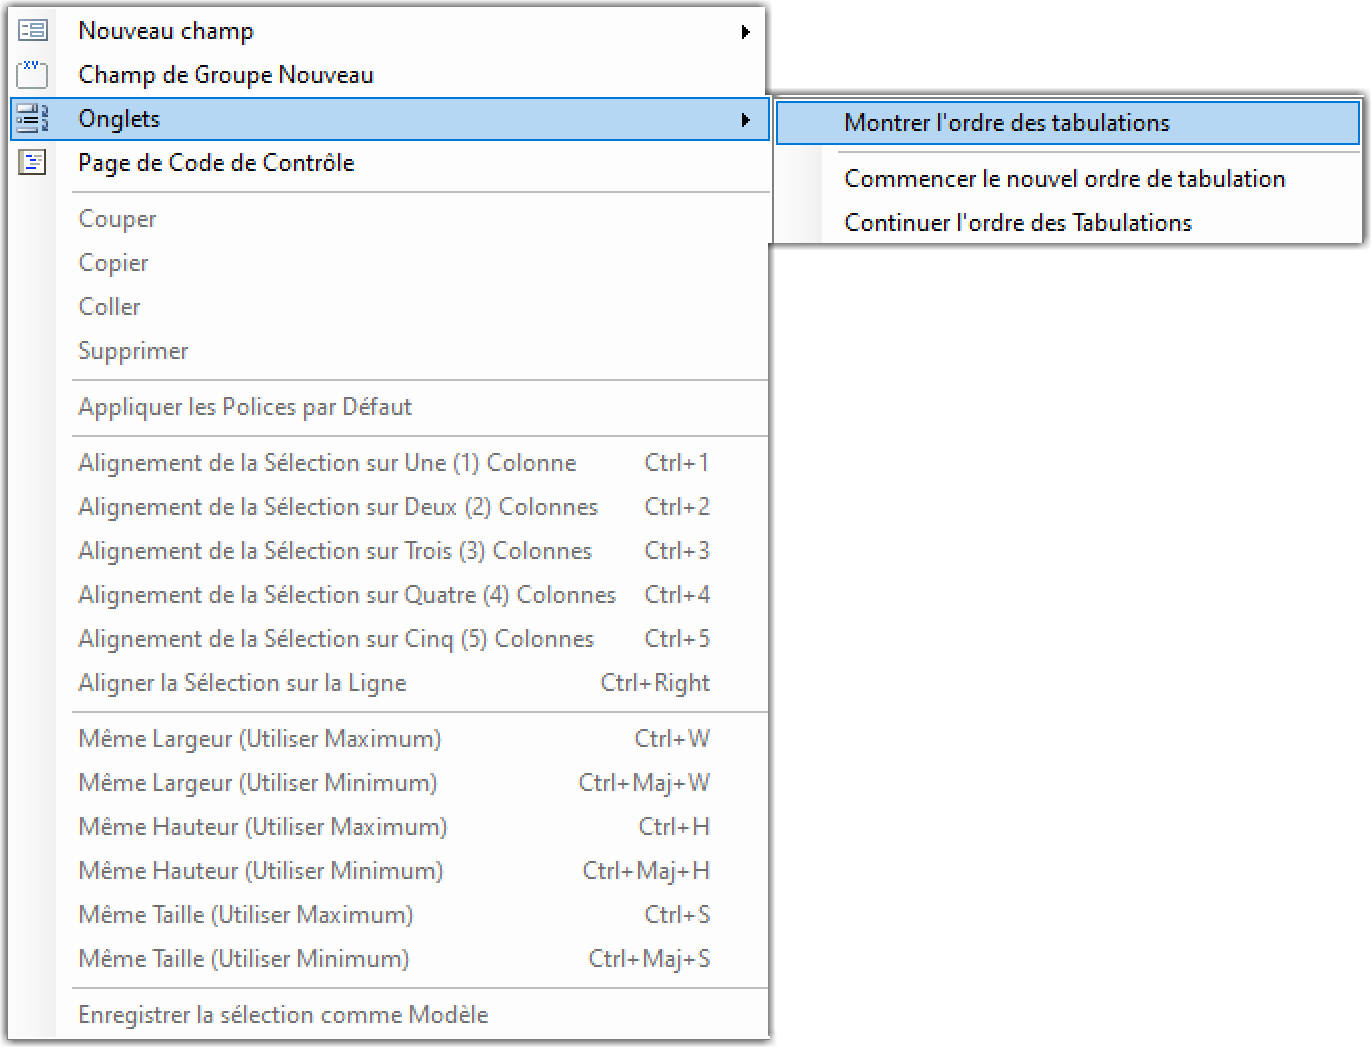
\includegraphics[width=\linewidth,height=0.4\textheight,keepaspectratio]{img/questionnaire/afficherOrdreTabulation}
	\caption{Affichage de l'ordre de tabulation}
	\label{fig:afficherordretabulation}
\end{figure}

\begin{figure}[H]
	\centering
	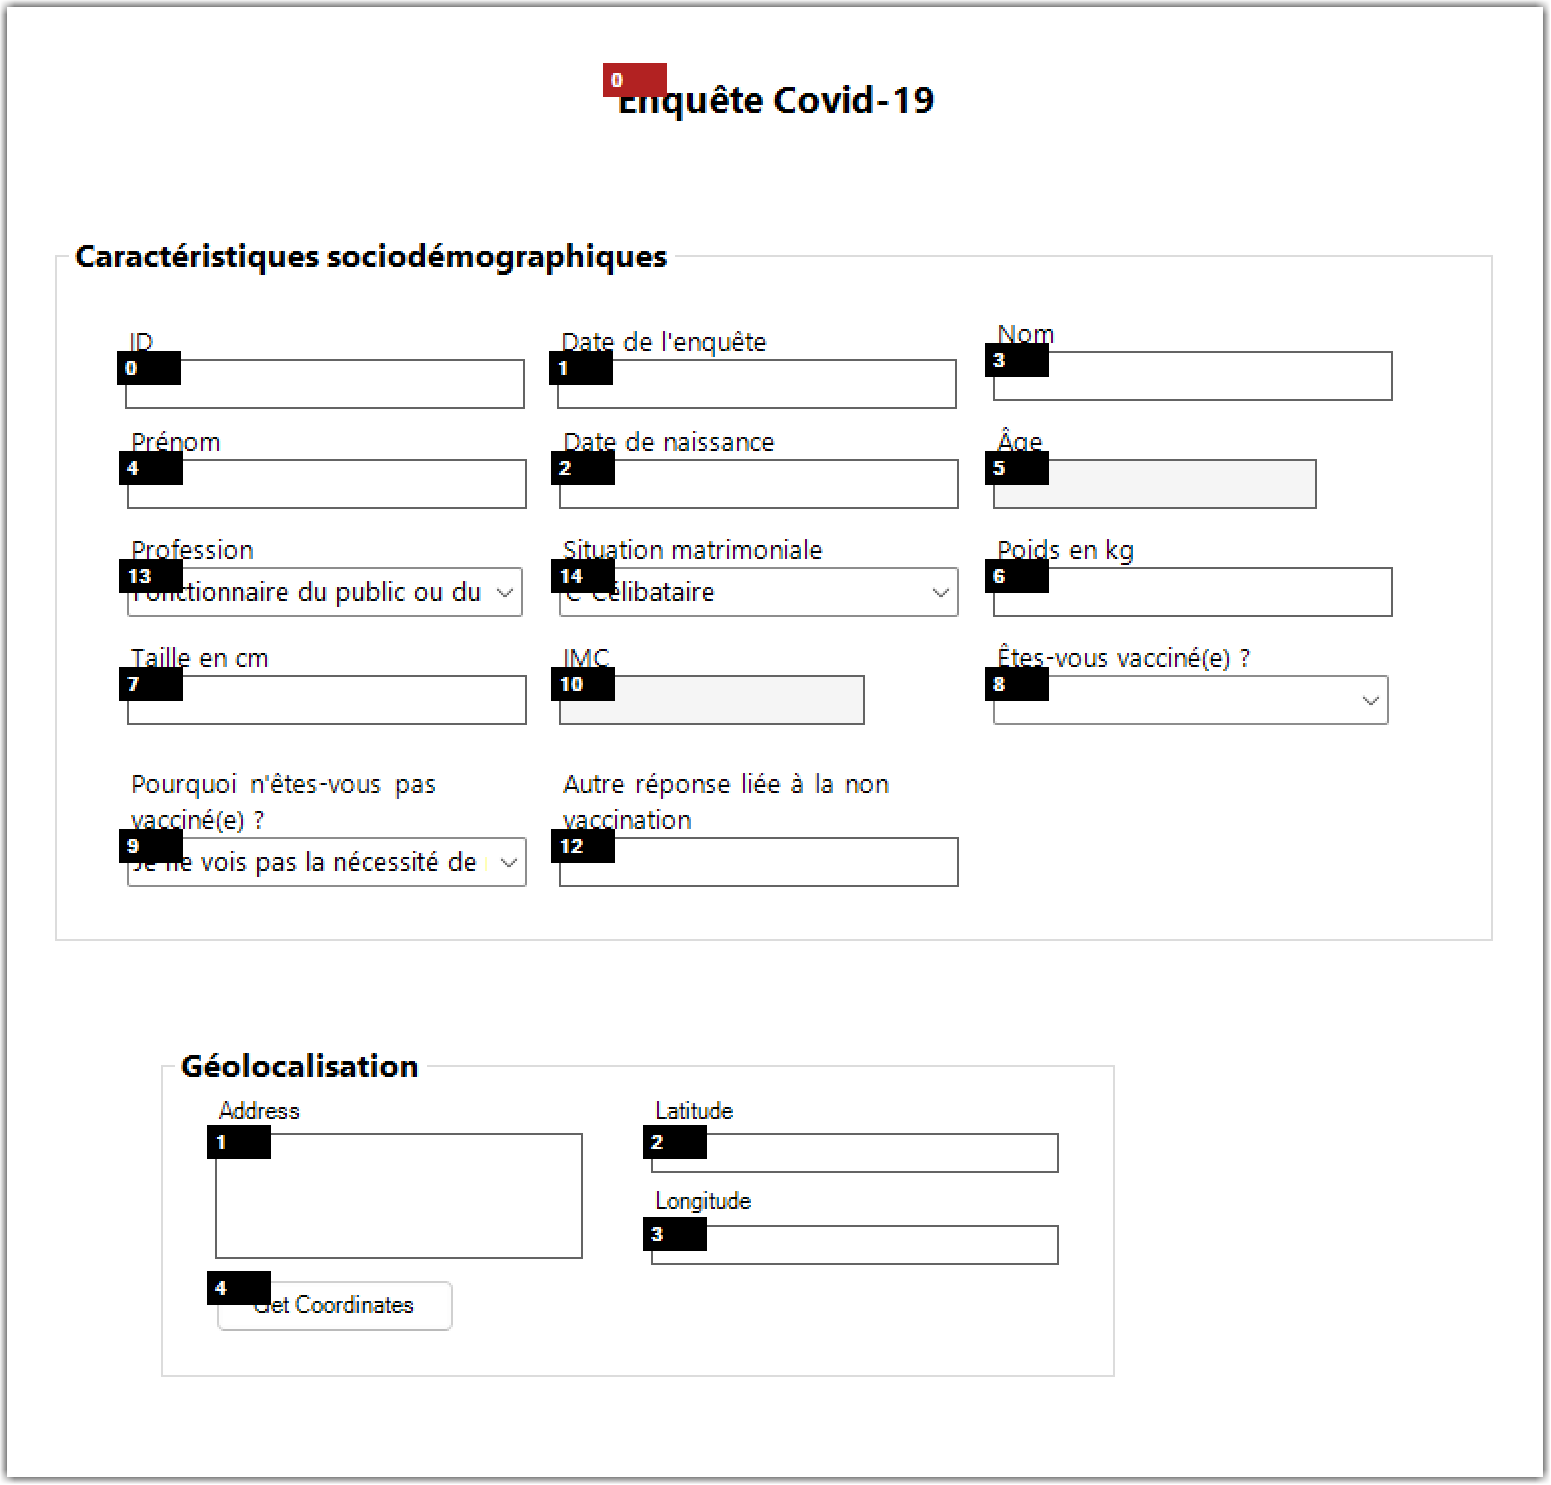
\includegraphics[width=\linewidth,height=0.4\textheight,keepaspectratio]{img/questionnaire/ordreTabulation}
	\caption{Ordre de tabulation existant}
	\label{fig:ordretabulation}
\end{figure}

Cet ordre ne nous convient pas ; nous allons donc le réorganiser. Faire de nouveau un clic droit sur le canevas, aller dans \kw{Onglets} et cliquer sur \kw{Commencer le nouvel ordre de tabulation}, puis cliquer sur les champs dans l'ordre souhaité. Pour ne changer l'ordre que de certains champs, cliquer sur le numéro correspondant au champ. La \autoref{fig:nouvelordretabulation} montre le nouvel ordre.

\begin{figure}[H]
	\centering
	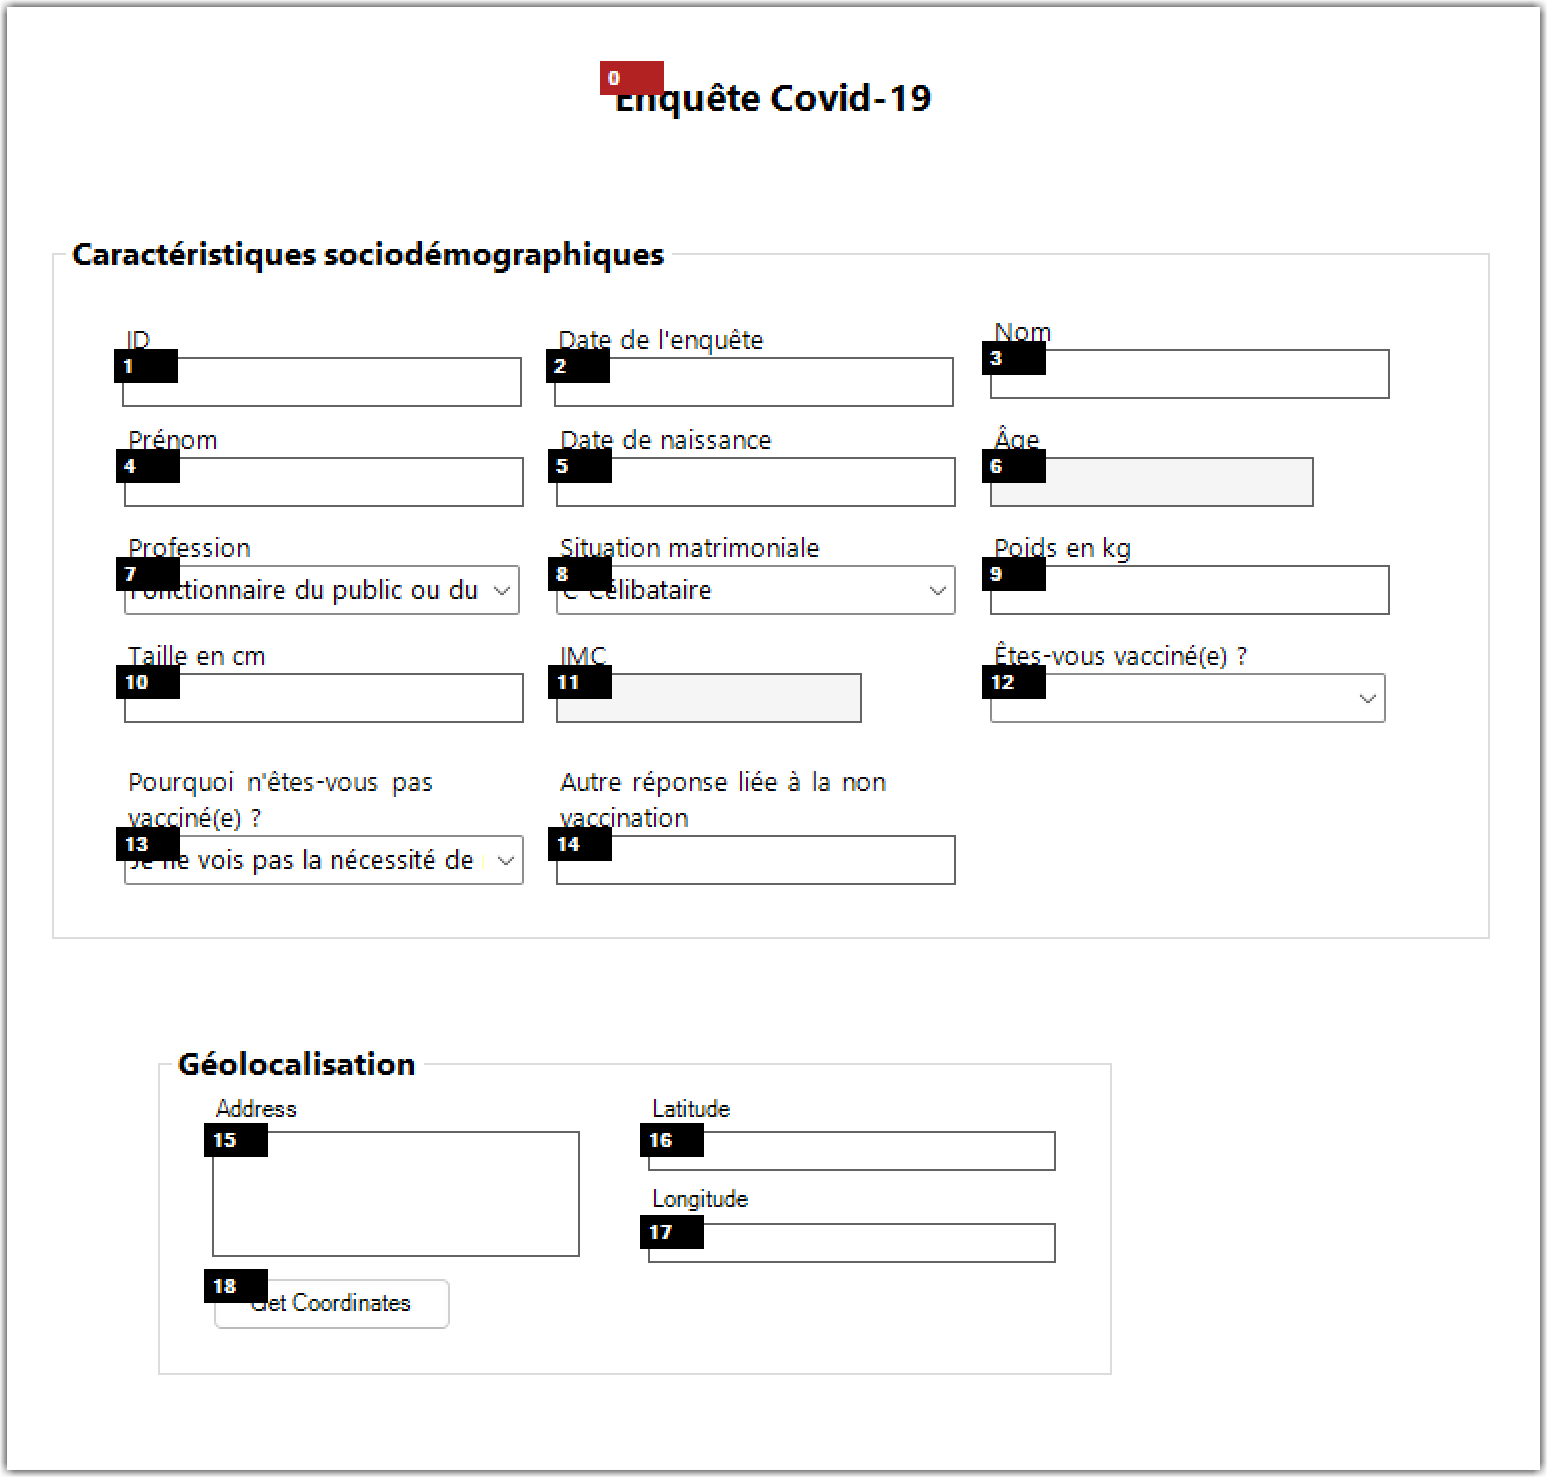
\includegraphics[width=\linewidth,height=0.4\textheight,keepaspectratio]{img/questionnaire/nouvelOrdreTabulation}
	\caption{Nouvel ordre de tabulation}
	\label{fig:nouvelordretabulation}
\end{figure}

\section{Utiliser des modèles}
\label{modeles}

Epi Info permet d'enregistrer des éléments d'un formulaire sous forme de modèles pour les réutiliser plus tard. Il existe deux sortes de modèles : le \terme{modèle de champs}, qui ne contient qu'une sélection de champs, et le \terme{modèle de projet}, qui contient le projet entier.

\subsection{Créer un modèle de champs}

Vous voudrez peut-être réutiliser certains champs dans des formulaires futurs. Plutôt que de recréer les mêmes champs, vous pouvez enregistrer votre sélection comme modèle. Vous gagnerez ainsi du temps et pourrez créer un formulaire très rapidement, en cas d'urgence par exemple.
Dans notre cas, nous voulons enregistrer comme modèle les champs nom, prénom, âge, profession, etc., que nous avons regroupés sous la bannière \question{Caractéristiques sociodémographiques}. Pour créer le modèle :

\begin{enumerate}
	\item Sélectionner avec la souris tous les champs à enregistrer, ici le groupe Caractéristiques sociodémographiques ;
	\item Faire un clic droit sur une partie vide du canevas. Un menu contextuel s'ouvre ;
	\item Cliquer sur \kw{Enregistrer la sélection comme modèle}. Une fenêtre nommée Ajouter un modèle apparaît ;
	\item Saisir le nom du modèle, ici \kw{Caractéristiques socio-démographiques} ;
	\item Valider par \kw{OK}.
\end{enumerate}

Le modèle créé apparaît dans l'explorateur de projets, dans la rubrique \kw{Modèles}, puis \kw{Fields} (\og champs \fg{} en français). La \autoref{fig:ajoutmodelechamp} montre que notre modèle a bien été créé. S'il n'apparaît pas, cliquer sur le $+$ à gauche de \kw{Modèles} puis de \kw{Fields} pour déplier la liste.

Pour ajouter ce modèle dans un futur formulaire, il suffit de le faire glisser\footnote{Le glisser-déposer consiste à cliquer sur un élément, à le déplacer vers une zone précise en maintenant le bouton de la souris enfoncé, puis à relâcher le bouton.} sur le canevas.

\begin{figure}[H]
	\centering
	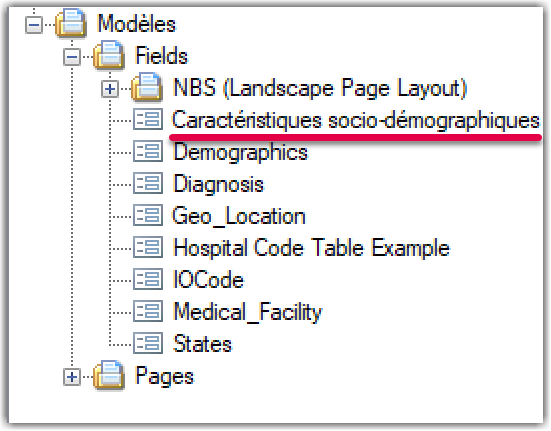
\includegraphics[width=0.55\linewidth]{img/questionnaire/ajoutModeleChamp}
	\caption{Ajouter un modèle de champs}
	\label{fig:ajoutmodelechamp}
\end{figure}

%% Ce fichier est inclus à la fin de la section « Utiliser des modèles »
%% du chapitre 3 (03creerQuestionnaire.tex), juste après le modèle de champs.

\subsection{Créer un modèle de projet}
\label{modeleProjet}

Contrairement au modèle de champs, le modèle de projet englobe l'ensemble du projet : tous ses formulaires, toutes les pages de chaque formulaire et tout le code de contrôle (que nous verrons au chapitre~\ref{codeValidation}). C'est ce modèle que l'on envoie aux enquêteurs pour qu'ils disposent tous exactement du même questionnaire. Pour créer un modèle de projet à partir de notre projet COVID19 :

\begin{enumerate}
	\item Dans l'explorateur de projets, faire un clic droit sur le nom du projet, ici \var{COVID19}. Un menu contextuel apparaît ;
	\item Sélectionner \kw{Enregistrer le projet en tant que modèle} (\emph{Save Project as Template}). La fenêtre du même nom s'ouvre ;
	\item Taper le nom du modèle, par exemple \var{ModeleCOVID19}, dans le champ \kw{Nom du modèle} ;
	\item Cliquer sur \kw{OK}.
\end{enumerate}

\subsection{Envoyer un modèle de projet à un collègue}

Une fois le modèle créé, il apparaît dans l'explorateur de projets, dans la rubrique \kw{Modèles}, sous \var{Projects}. Il ne reste plus qu'à retrouver le fichier pour le joindre à un courriel ou le copier sur une clé USB :

\begin{enumerate}
	\item Repérer le modèle \var{ModeleCOVID19} sous \var{Projects} dans l'explorateur de projets. Il faudra peut-être faire défiler le volet vers le bas pour le trouver ;
	\item Faire un clic droit sur \var{ModeleCOVID19}. Un menu contextuel apparaît ;
	\item Sélectionner \kw{Ouvrir le dossier conteneur} (\emph{Open Containing Folder}). Une fenêtre de l'Explorateur de fichiers de Windows s'ouvre ;
	\item Repérer le fichier \var{ModeleCOVID19.xml} dans la liste. Ce fichier est le modèle : vous pouvez le joindre à un courriel avec votre messagerie habituelle ou le copier sur une clé USB.
\end{enumerate}

\subsection{Charger un modèle de projet reçu d'un collègue}

Mettons-nous maintenant à la place d'un enquêteur qui vient de recevoir le fichier \var{ModeleCOVID19.xml} par courriel. Pour créer le projet à partir de ce modèle :

\begin{enumerate}
	\item Enregistrer la pièce jointe sur le bureau de l'ordinateur ;
	\item Ouvrir le module \module{créer questionnaires} d'Epi Info 7 ;
	\item Aller dans \kw{Fichier > Obtenir un modèle\ldots} Une fenêtre Windows d'ouverture de fichier apparaît ;
	\item Aller sur le bureau et sélectionner le fichier reçu ;
	\item Cliquer sur \kw{Ouvrir}. La fenêtre \kw{Nouveau projet à partir d'un modèle} s'ouvre ;
	\item Sélectionner le modèle que vous venez de charger, s'il ne l'est pas déjà ;
	\item Si nécessaire, indiquer un nom de projet dans la zone \kw{Nom} ;
	\item Cliquer sur \kw{OK} pour créer le projet.
\end{enumerate}

L'enquêteur dispose alors d'un projet identique au vôtre, prêt pour la saisie des données.

\begin{mybox}[colbacktitle=TIP]{\faLightbulb{} CONSEIL}
Créez et envoyez le modèle de projet seulement après avoir testé le questionnaire et son code de contrôle (chapitres~\ref{codeValidation} et~\ref{saisirDonnees}). Tous les enquêteurs travailleront ainsi sur la même version, et leurs données pourront être fusionnées sans difficulté.
\end{mybox}


\chapter{Utiliser le code de contrôle}
\label{codeValidation}
%\minitoc

Epi Info 7 dispose d'un mécanisme de validation des données appelé \emph{Check Code}, ou code de contrôle. Le code de contrôle rend le formulaire plus intelligent : son comportement peut changer au cours de la saisie. Il permet notamment de calculer automatiquement des valeurs comme l'âge ou l'IMC, d'appliquer des sauts de questions, d'afficher des messages ou des questions à l'utilisateur pendant la saisie, de remplir des champs et de masquer des champs.
Le code de contrôle se construit à l'aide de boîtes de dialogue disponibles dans le module \module{créer questionnaires}. C'est à nous de programmer le comportement que nous voulons donner à notre questionnaire.

\section{Ouvrir l'éditeur de code de contrôle}

Pour accéder au code de contrôle, il faut d'abord ouvrir un formulaire :

\begin{enumerate}
\item Ouvrir Epi Info 7 et aller dans le module \module{créer questionnaires} ;
\item Dans la barre d'outils, cliquer sur \kw{Fichier} puis sur \kw{Ouvrir le projet}. Vous pouvez aussi utiliser le raccourci clavier \kw{Ctrl + O} ;
\item Aller dans le répertoire des projets d'Epi Info 7 et ouvrir le dossier de notre projet \var{COVID19}, créé au chapitre~\ref{creerQuestionnaire} (il faudra peut-être faire défiler la liste pour l'apercevoir) ;
\item Ouvrir le fichier \var{COVID19.prj}, par un double-clic ou en le sélectionnant puis en cliquant sur \kw{Ouvrir} ;
\item Une fois le formulaire ouvert, cliquer sur le bouton \kw{Code de contrôle}, qui ouvre l'éditeur de code de contrôle (\autoref{fig:editeurcodevalidation}).
\end{enumerate}

\begin{figure}[H]
	\centering
	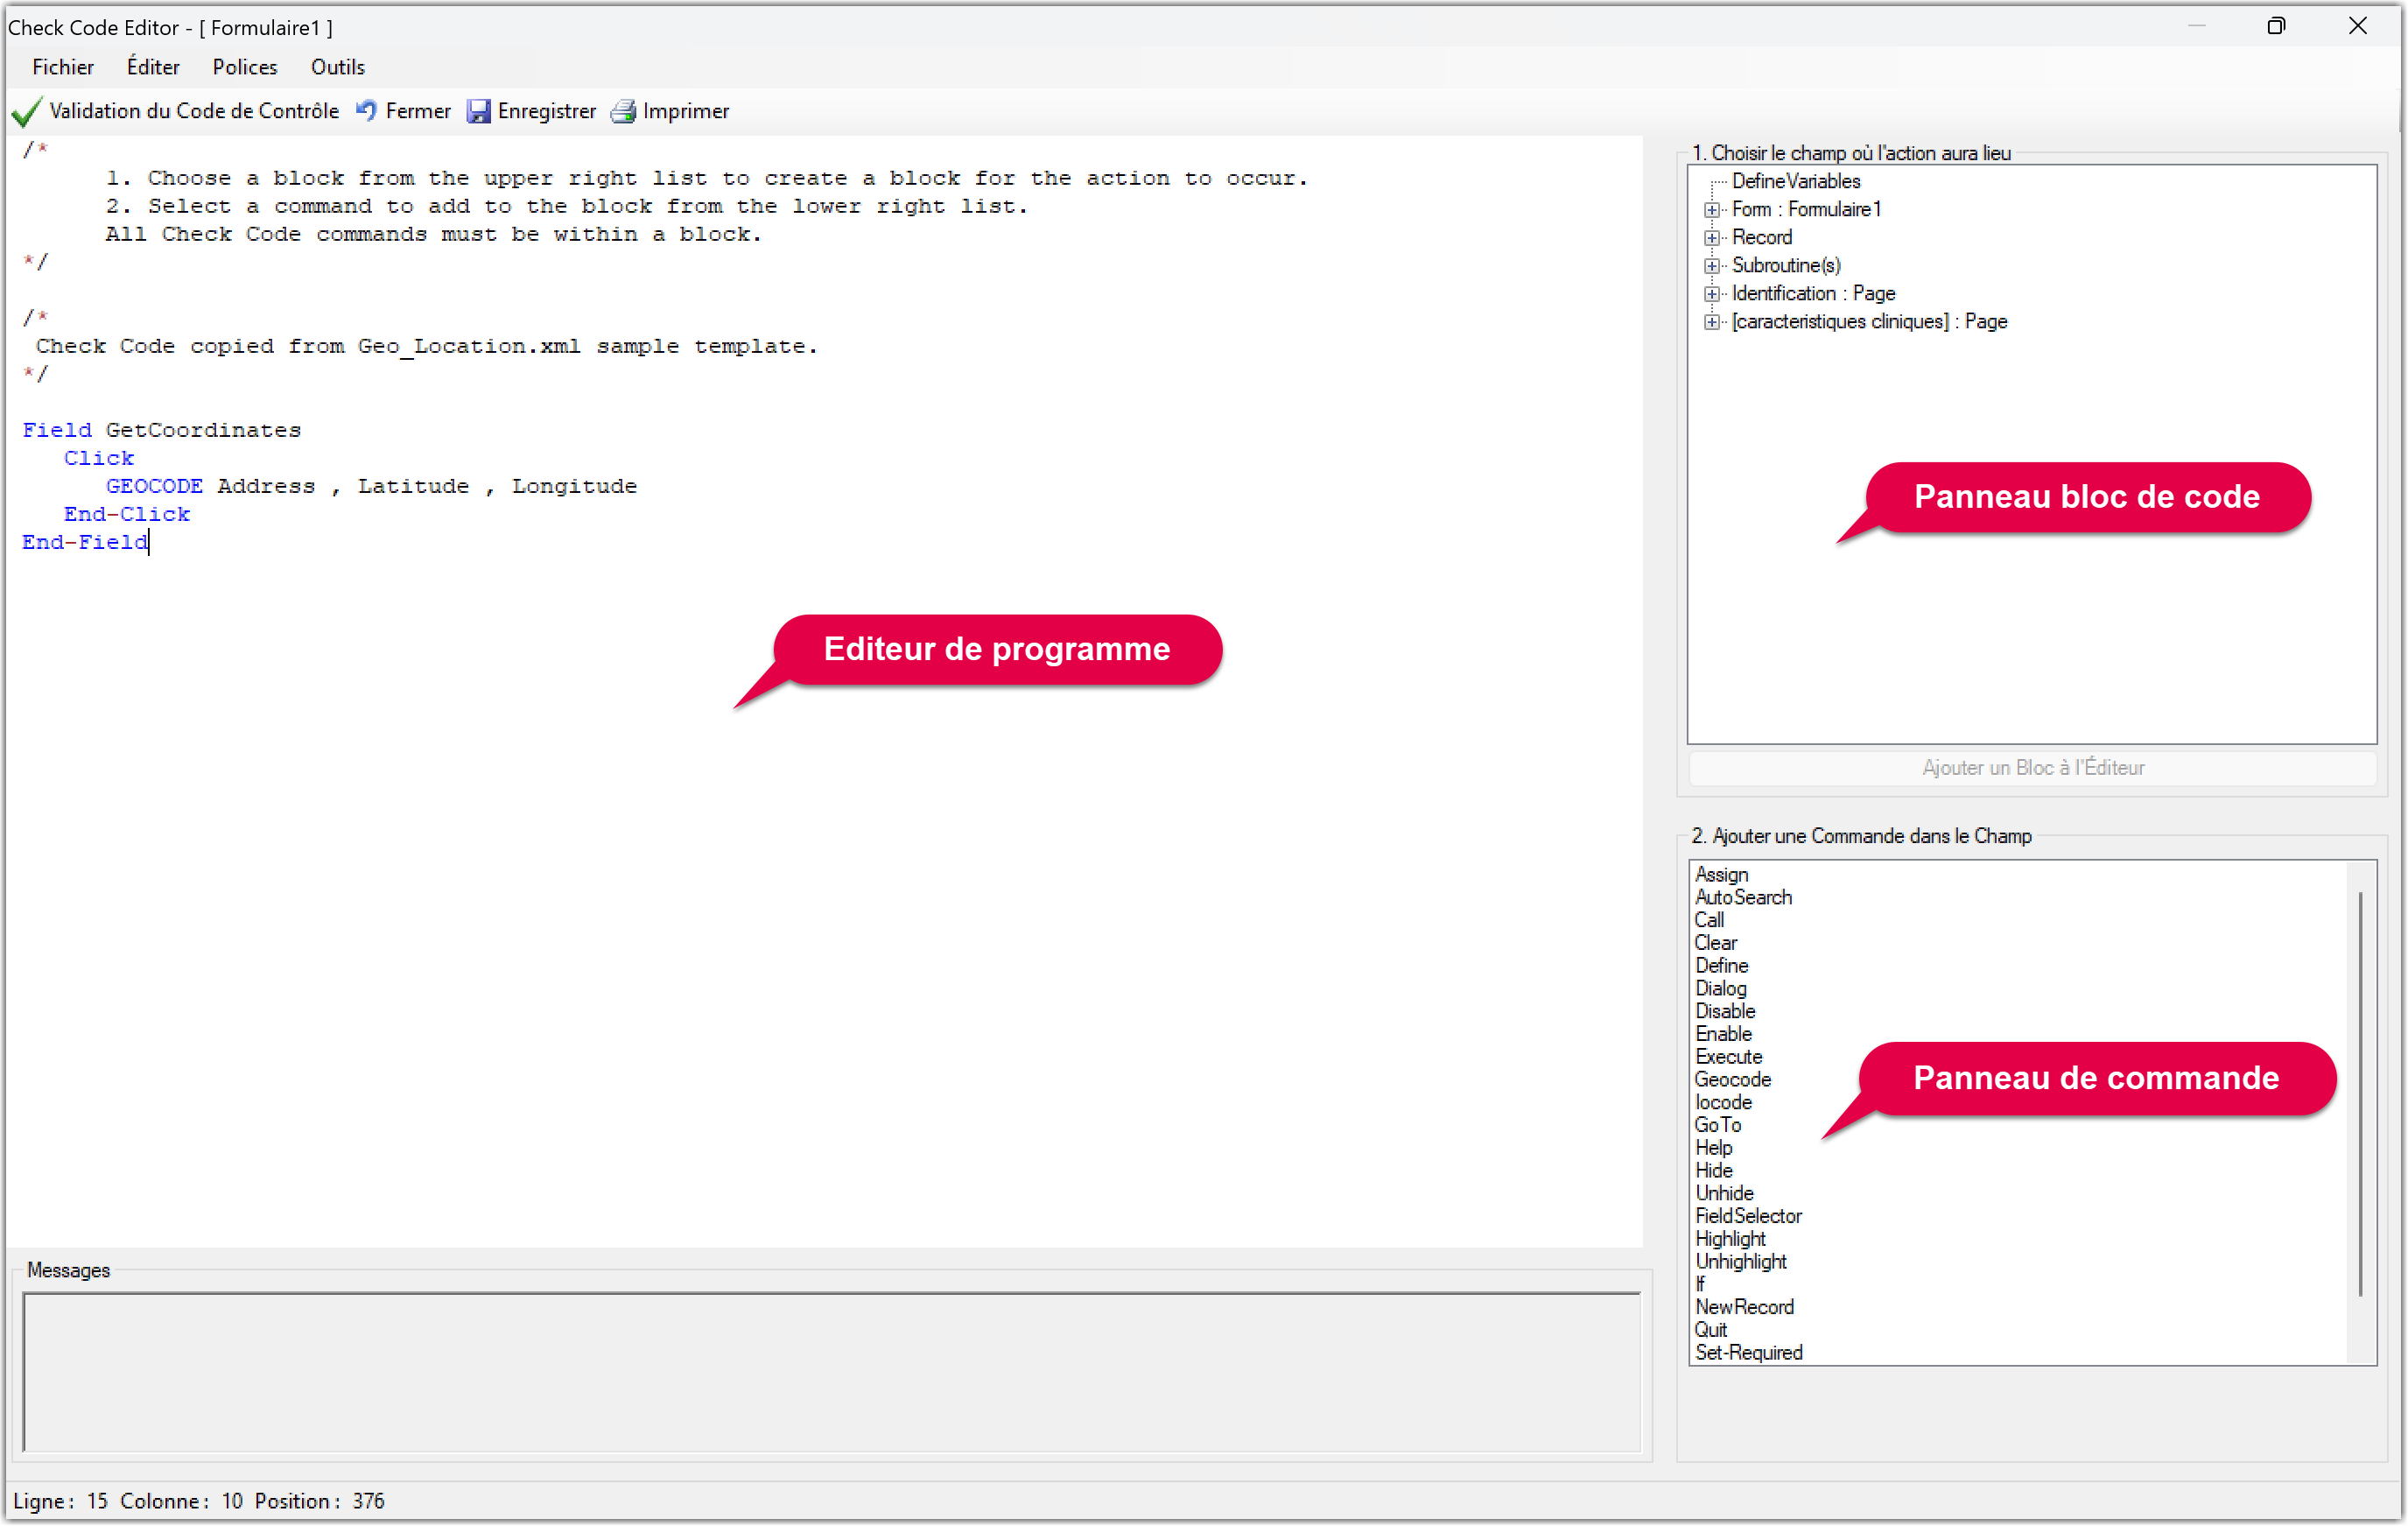
\includegraphics[width=\linewidth,height=0.4\textheight,keepaspectratio]{img/CodeValidation/editeurCodeValidation}
	\caption{Éditeur du code de contrôle}
	\label{fig:editeurcodevalidation}
\end{figure}

Tout code de contrôle doit être associé à un champ existant du formulaire. Les champs disponibles sont listés, page par page, dans le panneau \kw{Choisir le champ où l'action aura lieu}.

Le code de contrôle repose sur des événements : nous définissons le comportement des champs en fonction d'actions comme l'ouverture ou la fermeture du formulaire, l'ouverture ou la fermeture d'une page, l'entrée du curseur dans un champ (\commande{Before}) ou sa sortie (\commande{After}).

\begin{mybox}[colbacktitle=NOTE]{\faInfoCircle{} À RETENIR}
Dans l'éditeur, vous ne verrez pas l'intitulé de vos questions mais le nom des variables, c'est-à-dire ce que vous avez saisi dans \kw{Nom du champ}. D'où l'importance, une fois de plus, de bien nommer ses variables.
\end{mybox}

\section{Les principales commandes}

Dans ce chapitre, nous voulons calculer automatiquement l'âge de la personne enquêtée à partir de sa date de naissance et de la date de l'enquête. Epi Info 7 calcule la différence entre deux dates en années, en mois ou en jours, avec respectivement les fonctions \commande{YEARS()}, \commande{MONTHS()} et \commande{DAYS()}. De même, au lieu de calculer l'indice de masse corporelle (IMC) à la main, nous voulons le déduire du poids et de la taille. Rappelons que l'IMC est égal au poids en kilogrammes divisé par le carré de la taille en mètres. La taille étant saisie en centimètres, nous la divisons par 100 :
\[
\text{IMC} = \frac{\text{poids\_kg}}{\left(\text{taille\_cm}/100\right)^2}
\]

Voici les commandes du code de contrôle que nous utiliserons le plus :

\begin{itemize}[label=\ding{45}]
	\item \commande{DEFINE} (Définir) : crée une nouvelle variable ;
	\item \commande{ASSIGN} (Attribuer) : affecte à une variable le résultat d'une opération arithmétique ou d'une expression de texte ;
	\item \commande{HIDE} (Masquer) : masque un champ pour le rendre invisible ;
	\item \commande{UNHIDE} (Afficher) : rend visible un champ masqué auparavant ;
	\item \commande{DISABLE} (Désactiver) : désactive un champ. Un champ désactivé n'accepte aucune saisie et sort de l'ordre de tabulation ;
	\item \commande{ENABLE} (Activer) : réactive un champ désactivé auparavant ;
	\item \commande{IF} (Si) : définit une condition et ce qui doit se passer si elle est remplie. Une autre action peut être prévue après l'instruction \commande{ELSE} (Sinon) ;
	\item \commande{GOTO} (Aller à) : seul ou dans une instruction If, envoie le curseur vers un champ ou une page ;
	\item \commande{CLEAR} (Effacer) : vide le champ indiqué, comme s'il n'avait jamais été rempli ;
	\item \commande{DIALOG} (Boîte de dialogue) : affiche un message à l'utilisateur.
\end{itemize}

\section{La commande Assign}

Dans notre questionnaire, l'âge doit être déduit de la date de naissance et de la date de l'enquête, et l'IMC du poids et de la taille. Nous voulons donc affecter aux variables \var{age} et \var{imc} une formule de calcul : c'est le rôle de la commande \commande{ASSIGN}.

Une fois dans l'éditeur de code de contrôle, procéder comme suit pour remplir automatiquement le champ \var{age} (\autoref{fig:creercodevalidationage}) :

\begin{enumerate}
	\item Dans le panneau des blocs de code, cliquer sur le $+$ à côté de \kw{Identification : Page} pour déplier les champs de la page Identification (étape 1) ;
	\item Cliquer sur le $+$ à gauche de la variable \var{age} (étape 2) ;
	\item Cliquer sur \commande{After} (étape 3) : l'action aura lieu à la sortie du champ ;
	\item Cliquer sur \kw{Ajouter un bloc} pour ajouter le bloc de code dans l'éditeur de programme (étape 4) ;
	\item Dans le panneau des commandes, cliquer sur la commande \commande{ASSIGN}. Une fenêtre apparaît (étape 5) ;
	\item Cliquer sur la flèche déroulante \kw{Assigner variable} et choisir la variable \var{age} (étape 6) ;
	\item Dans la partie \kw{Expression}, cliquer sur le petit rectangle $f(x)$ (étape 7) ;
	\item Dans le menu qui s'ouvre, aller à \kw{Fonctions Date} (étape 8) ;
	\item Dans le dernier sous-menu, choisir la fonction \commande{YEARS()} (étape 9).
\end{enumerate}

\begin{figure}[H]
	\centering
	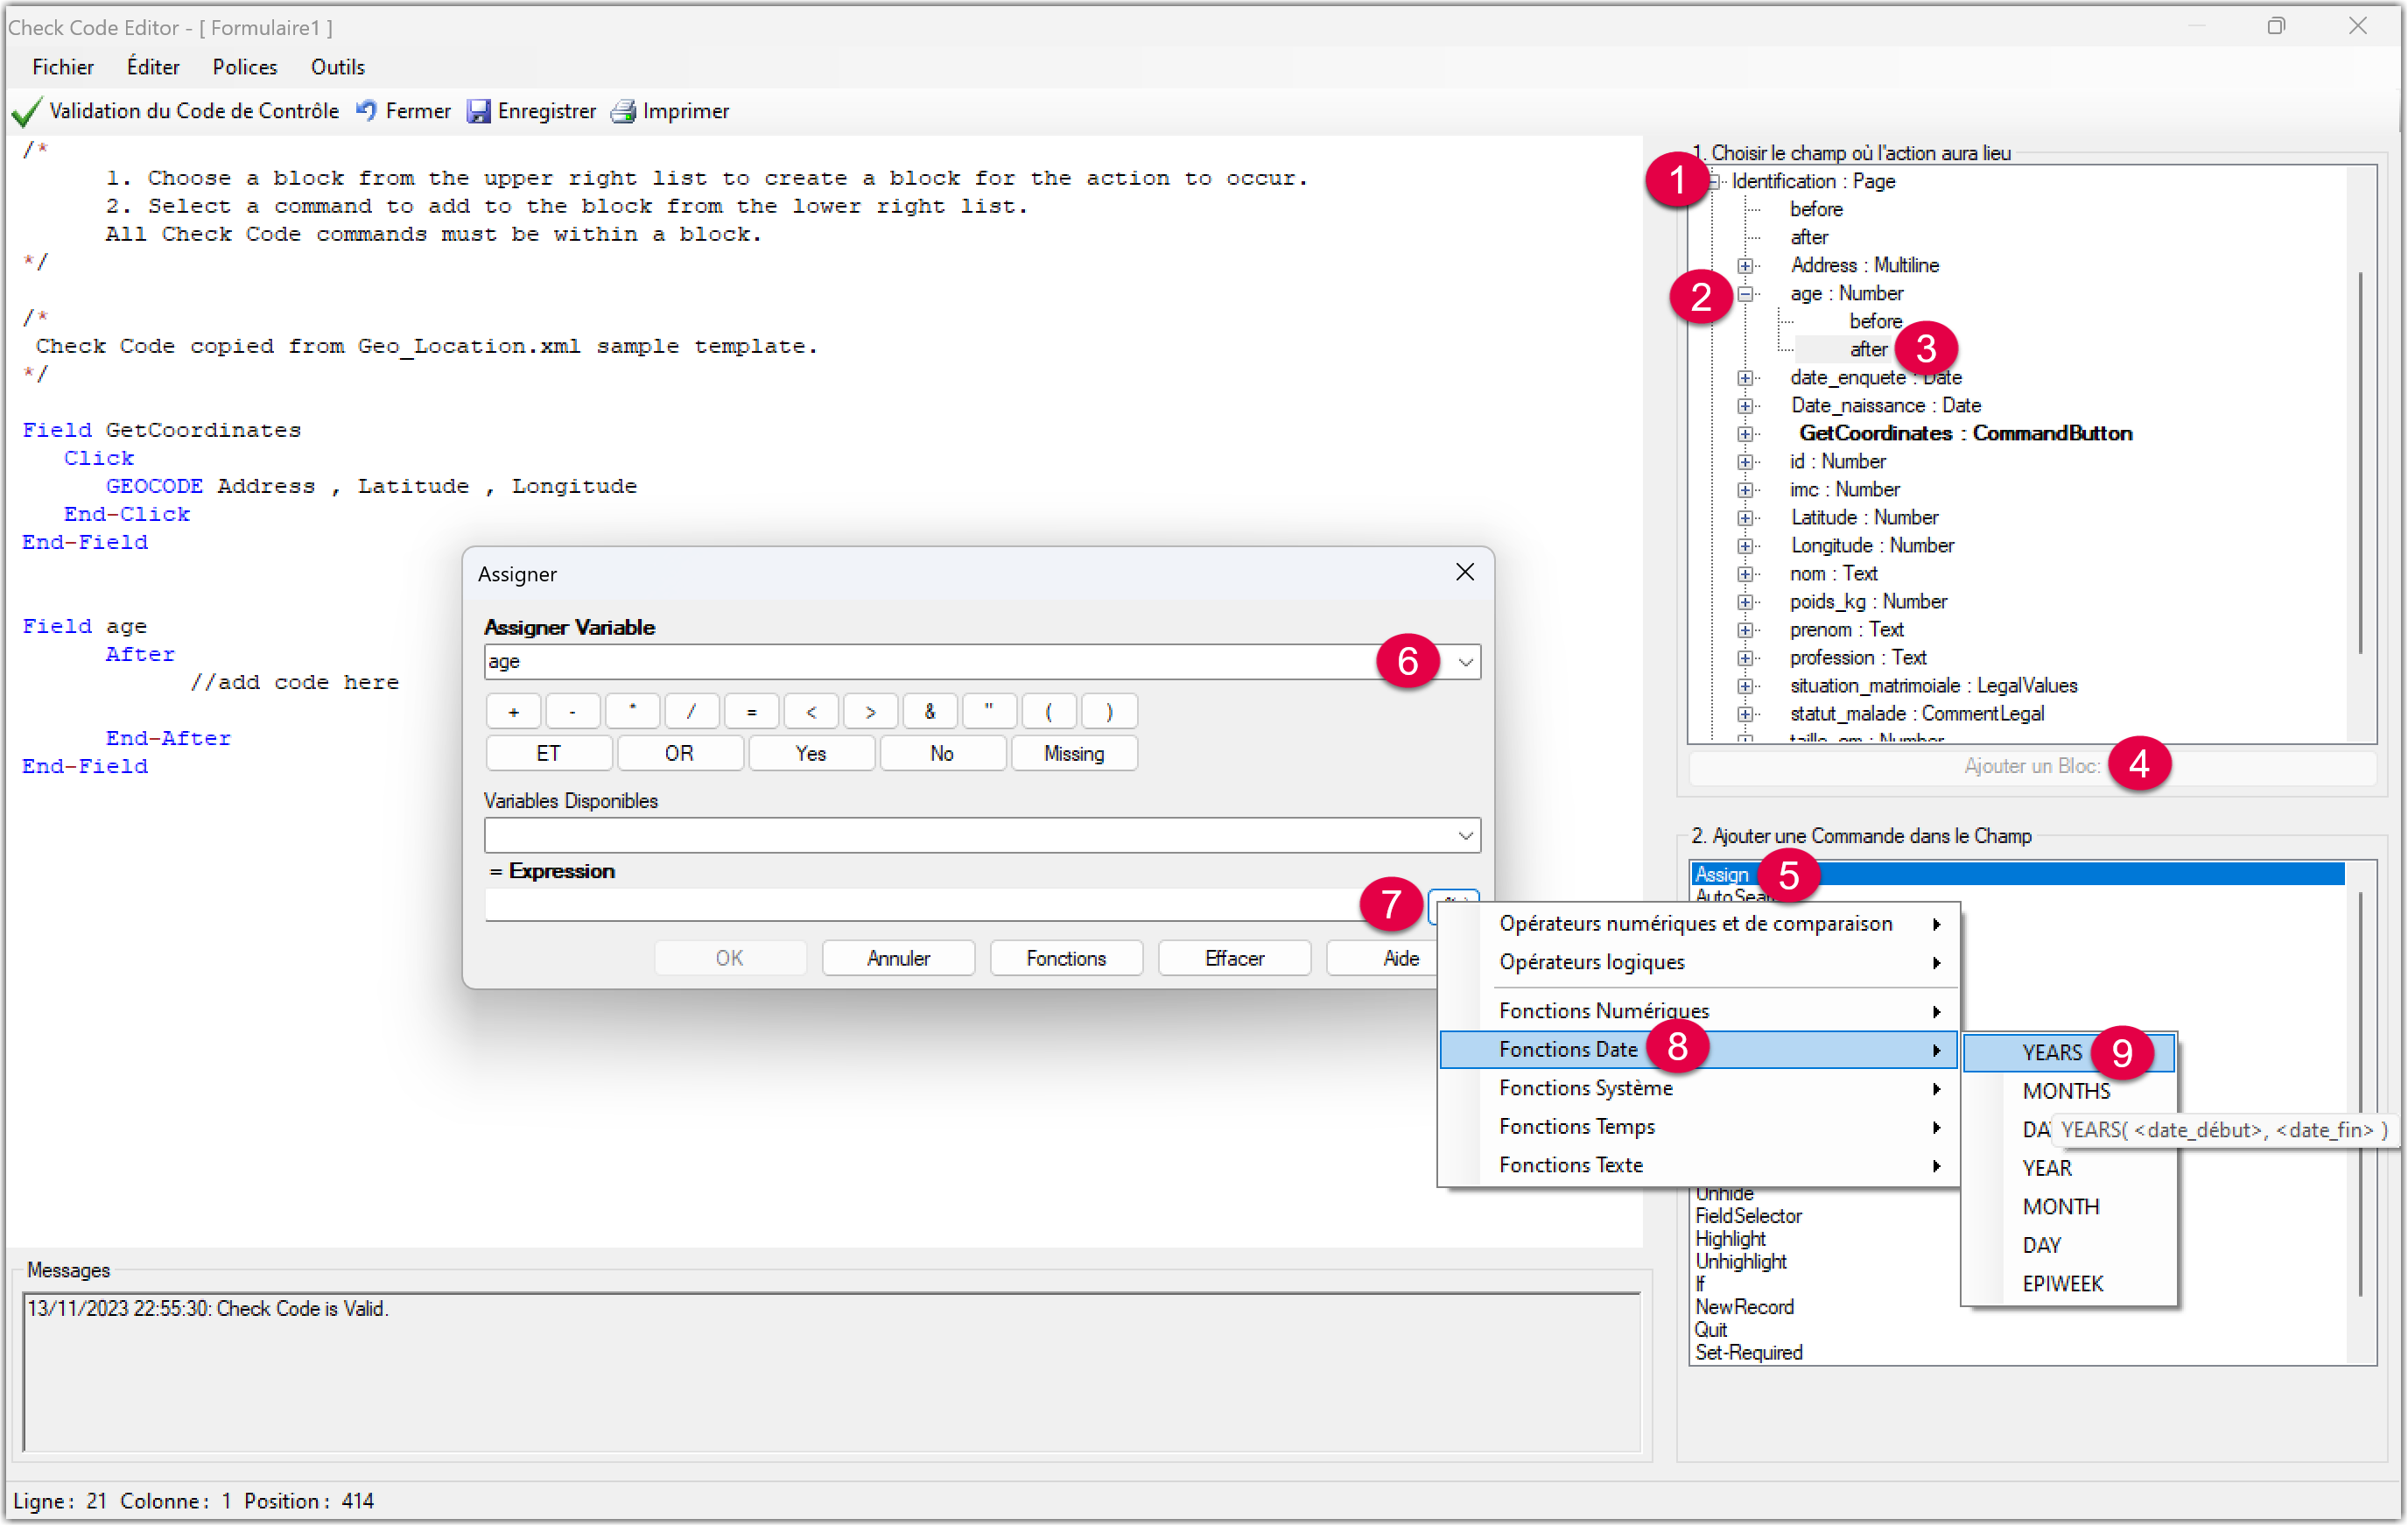
\includegraphics[width=\linewidth,height=0.4\textheight,keepaspectratio]{img/CodeValidation/creerCodeValidationAge}
	\caption{Création d'un code de contrôle pour le champ âge}
	\label{fig:creercodevalidationage}
\end{figure}

L'expression générique de la fonction s'affiche alors : \commande{YEARS(date\_debut, date\_fin)}. Nous la complétons avec nos variables (\autoref{fig:ecrituredelalogiqueage}) :
\begin{enumerate}
	\item Double-cliquer sur \var{date\_debut} pour le sélectionner ;
	\item À l'aide de la flèche déroulante \kw{Variables disponibles}, choisir la variable \var{date\_naissance} ;
	\item Double-cliquer sur \var{date\_fin} ;
	\item Dans la liste \kw{Variables disponibles}, choisir la variable \var{date\_enquete} ;
	\item Valider le tout par \kw{OK} (\autoref{fig:codeassign}).
\end{enumerate}

\begin{figure}[H]
	\centering
	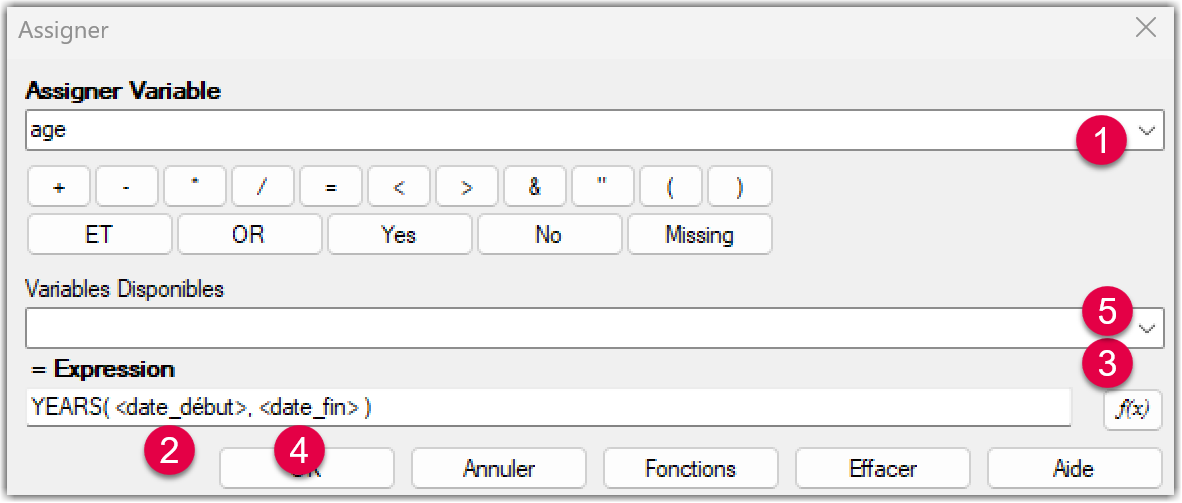
\includegraphics[width=\linewidth,height=0.4\textheight,keepaspectratio]{img/CodeValidation/ecritureDeLaLogiqueAge}
	\caption{Écriture de l'expression de la fonction YEARS()}
	\label{fig:ecrituredelalogiqueage}
\end{figure}

\begin{figure}[H]
	\centering
	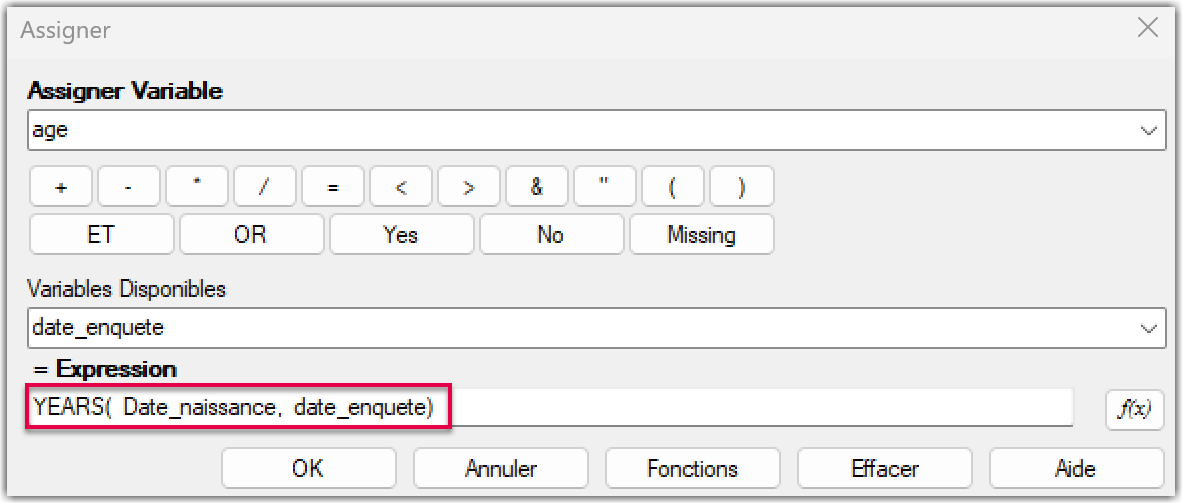
\includegraphics[width=\linewidth,height=0.4\textheight,keepaspectratio]{img/CodeValidation/codeAssign}
	\caption{Fonction YEARS()}
	\label{fig:codeassign}
\end{figure}

Après validation, le code apparaît dans l'éditeur de programme (\autoref{lst:assign}, page~\pageref{lst:assign}). Il reste à vérifier que le code est valide en cliquant, en haut à gauche, sur \kw{Valider le code de contrôle}\footnote{Un message s'affiche en bas, dans la zone \kw{Messages}, avec la date, l'heure et la mention \commande{Check Code is Valid} si le code est valide. Sinon, une erreur est signalée.}, puis à l'enregistrer en cliquant sur \kw{Enregistrer}.

\begin{tcolorbox}[drop lifted shadow]
	\begin{lstlisting}[language=EPIscript, style=mystyle, caption={Utilisation de la fonction YEARS() avec la commande ASSIGN}, label=lst:assign]
Field age
	After
		//add code here
		ASSIGN age = YEARS(date_naissance, date_enquete)
	End-After
End-Field
	\end{lstlisting}
\end{tcolorbox}

Nous créons de la même manière le code de contrôle de la variable \var{imc} (\autoref{fig:assignationimc}) :

\begin{enumerate}
	\item Dans le panneau des blocs de code, chercher la variable \var{imc}, qui se trouve sur la page Identification du formulaire ;
	\item Cliquer sur le $+$ à gauche de la variable \var{imc}, puis sur \commande{After} ;
	\item Cliquer sur \kw{Ajouter un bloc} ;
	\item Cliquer sur la commande \commande{ASSIGN} dans le panneau des commandes et choisir la variable \var{imc} ;
	\item Dans la partie \kw{Expression}, écrire la formule de l'IMC en vous aidant de la liste \kw{Variables disponibles}. N'oubliez pas de diviser la taille par 100 pour la convertir en mètres, puisque nous avons choisi de recueillir les tailles en centimètres ;
	\item Valider par \kw{OK} : le code apparaît dans l'éditeur de programme (\autoref{lst:imc}, page~\pageref{lst:imc}) ;
	\item Vérifier la validité du code en cliquant sur \kw{Valider le code de contrôle} ;
	\item Enregistrer le code en cliquant sur \kw{Enregistrer}.
\end{enumerate}

\begin{figure}[H]
	\centering
	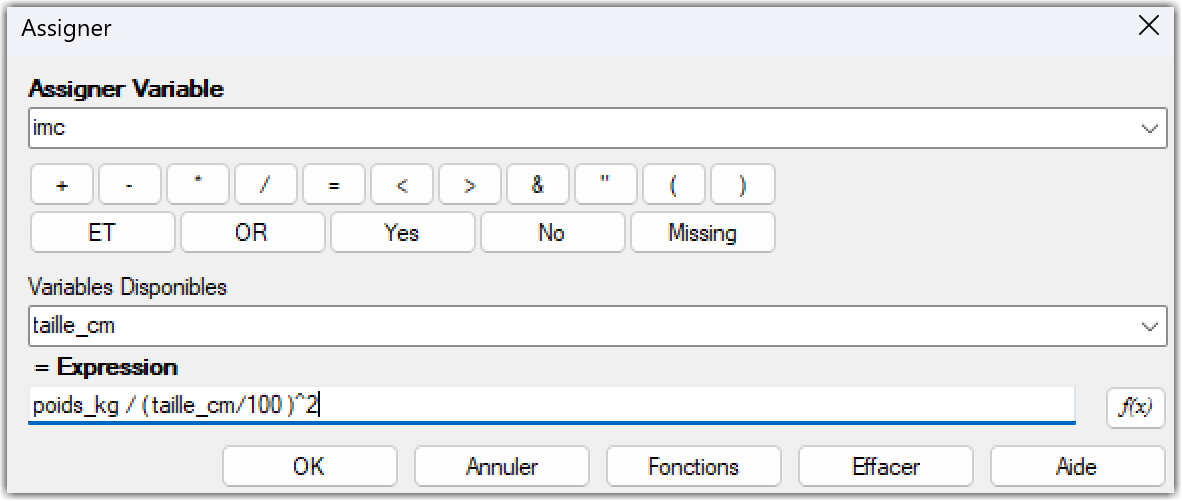
\includegraphics[width=\linewidth,height=0.4\textheight,keepaspectratio]{img/CodeValidation/assignationIMC}
	\caption{Création du code de contrôle de la variable imc}
	\label{fig:assignationimc}
\end{figure}

\begin{tcolorbox}[drop lifted shadow]
	\begin{lstlisting}[language=EPIscript, style=mystyle, caption={Code d'assignation de la variable imc}, label=lst:imc]
Field imc
	After
		//add code here
		ASSIGN imc = poids_kg/(taille_cm/100)^2
	End-After
End-Field
	\end{lstlisting}
\end{tcolorbox}

\begin{mybox}[colbacktitle=IMPORTANT]{\faExclamationCircle{} IMPORTANT}
	\begin{itemize}[label=\ding{97}, font=\color{IMPORTANT}]
	\item En informatique en général, et dans Epi Info en particulier, les opérations arithmétiques s'écrivent $+$, $-$, $*$ et $/$ pour l'addition, la soustraction, la multiplication et la division. Le symbole \textcolor{IMPORTANT}{\texttt{\^{}}} représente la puissance ;
	\item Vérifiez toujours la validité du code ;
	\item Enregistrez toujours le code avant de quitter l'éditeur de code de contrôle.
\end{itemize}
\end{mybox}

\section{Les commandes If, Dialog, Clear et GoTo}

La commande \commande{IF} est utilisée en algorithmique et dans de nombreux langages de programmation pour exécuter une action sous condition. Elle s'emploie le plus souvent sous la forme \commande{IF} (condition) \commande{THEN} (action) \commande{ELSE} (autre action), soit : \og si la condition est vérifiée, exécuter ce bloc de code ; sinon, exécuter cet autre bloc \fg{}. Passons sans plus tarder à la démonstration.

Nous allons écrire un code simple qui nous alerte si nous saisissons par erreur une taille inférieure ou égale à 0~cm ou supérieure ou égale à 300~cm. Le code affiche alors une fenêtre intitulée \og Attention ! \fg{} avec le message \question{La taille saisie est incorrecte}, efface la valeur saisie et replace le curseur dans le champ pour une nouvelle saisie. Procédons comme suit (\autoref{fig:codeconditionsi}, page~\pageref{fig:codeconditionsi}) :

\begin{enumerate}
	\item Ouvrir l'éditeur de code de contrôle ;
	\item Dans le panneau des blocs de code, chercher la variable \var{taille\_cm}, située sur la page \kw{Identification} du formulaire ;
	\item Cliquer sur le $+$ pour déplier les événements de cette variable ;
	\item Cliquer sur \commande{After} puis sur \kw{Ajouter un bloc} ;
	\item Dans le panneau des commandes, cliquer sur la commande \commande{IF}. Une fenêtre s'ouvre ;
	\item Écrire la condition dans la case \kw{Condition Si}. On peut s'aider de la liste \kw{Variables disponibles} et du bouton de fonctions $f(x)$ ;
	\item Dans la partie \kw{Alors}, indiquer le code à exécuter lorsque la condition est vérifiée. Ici, nous ajoutons les commandes \commande{DIALOG}, \commande{CLEAR} et \commande{GOTO} en cliquant à chaque fois sur le petit symbole de document, dans le coin droit de la partie \kw{Alors} (étape \textcolor{IMPORTANT}{\Large \ding{204}} de la \autoref{fig:codeconditionsi}) ;
	\item On peut aussi utiliser la partie \kw{Sinon} (\commande{ELSE}) pour indiquer le code à exécuter lorsque la condition n'est pas vérifiée ;
	\item Cliquer sur \kw{OK} pour afficher le code créé dans l'éditeur de programme, puis le valider et l'enregistrer.
\end{enumerate}

\begin{figure}[H]
	\centering
	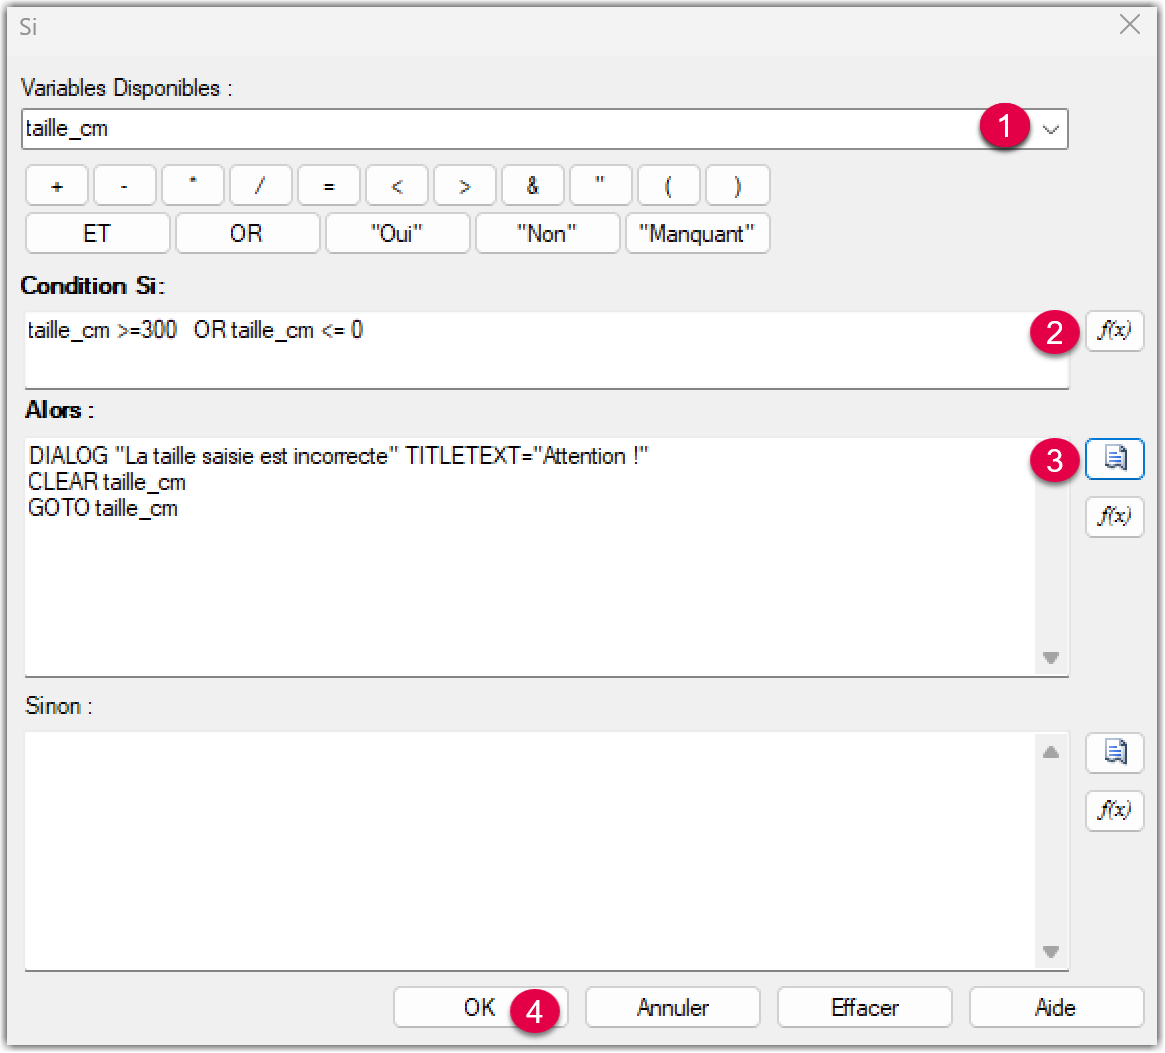
\includegraphics[width=\linewidth,height=0.4\textheight,keepaspectratio]{img/CodeValidation/codeConditionSi}
	\caption{Utilisation de la commande IF}
	\label{fig:codeconditionsi}
\end{figure}

Le code obtenu est présenté dans le \autoref{lst:dialog}, page~\pageref{lst:dialog}.

\begin{tcolorbox}[drop lifted shadow]
	\begin{lstlisting}[language=EPIscript, style=mystyle, caption={Code de contrôle de la variable taille\_cm}, label=lst:dialog]
Field taille_cm
	After
		//add code here
		IF taille_cm >= 300 OR taille_cm <= 0 THEN
			DIALOG "La taille saisie est incorrecte" TITLETEXT="Attention !"
			CLEAR taille_cm
			GOTO taille_cm
		END-IF
	End-After
End-Field
	\end{lstlisting}
\end{tcolorbox}

\paragraph{Explication du code}

\begin{itemize}
	\item Le code du champ est délimité par \commande{Field} (suivi du nom de la variable) et \commande{End-Field} ;
	\item \commande{After} \ldots{} \commande{End-After} indique que le code s'exécute à la sortie du champ. La ligne \textit{//add code here} est un simple commentaire ;
	\item La commande If est délimitée par \commande{IF} et \commande{END-IF} ;
	\item La condition \commande{taille\_cm >= 300 OR taille\_cm <= 0 THEN} signifie : SI la taille en centimètres est supérieure ou égale à 300 OU inférieure ou égale à 0, ALORS\ldots ;
	\item Le corps du bloc contient le code à exécuter, que nous expliquons ligne par ligne :
		\begin{itemize}[label=\ding{45}]
			\item \commande{DIALOG} : ouvre une fenêtre intitulée \og Attention ! \fg{} qui affiche le message \question{La taille saisie est incorrecte} ;
			\item \commande{CLEAR taille\_cm} : efface la valeur saisie dans le champ \var{taille\_cm} ;
			\item \commande{GOTO taille\_cm} : laisse le curseur dans le champ \var{taille\_cm} afin de pouvoir saisir à nouveau la taille.
		\end{itemize}
\end{itemize}

\section{Les commandes Enable et Disable}

Nous allons maintenant créer un code de contrôle plus élaboré, qui combine la commande \commande{IF-ELSE} avec les commandes \commande{ENABLE} et \commande{DISABLE}.

Dans notre questionnaire, nous voulons lier les questions \question{Êtes-vous vacciné(e) ?}, \question{Pourquoi n'êtes-vous pas vacciné(e) ?} et \question{Autre réponse liée à la non-vaccination}.

\begin{tcolorbox}[title=Description de la logique, drop small lifted shadow=black]

Si la réponse à la question \question{Êtes-vous vacciné(e) ?} (variable \var{vaccination}) est \kw{No} (\kw{Non}),\newline
alors le champ \question{Pourquoi n'êtes-vous pas vacciné(e) ?} (variable \var{pourquoi\_pas\_vaccine}) est activé pour permettre de choisir l'une des réponses proposées :
\begin{itemize}
	\item Je ne vois pas la nécessité de me faire vacciner ;
	\item Je ne fais pas confiance au vaccin ;
	\item Autre réponse.
\end{itemize}

Si la réponse choisie est \kw{Autre réponse}, alors le champ \question{Autre réponse liée à la non-vaccination} (variable \var{autre\_reponse\_non\_vaccination}) est activé pour permettre de la préciser.

En revanche, si la réponse à la question \question{Êtes-vous vacciné(e) ?} est \kw{Yes} (\kw{Oui}), les champs \question{Pourquoi n'êtes-vous pas vacciné(e) ?} et \question{Autre réponse liée à la non-vaccination} sont désactivés.

Notons que nous avons rendu le champ \question{Êtes-vous vacciné(e) ?} obligatoire en cochant \kw{Requis} lors de sa création.
\end{tcolorbox}

Ouvrons l'éditeur de code de contrôle et procédons comme suit (\autoref{fig:codeifenabledisable}, page~\pageref{fig:codeifenabledisable}) :

\begin{enumerate}
	\item Dans le panneau des blocs de code, double-cliquer sur la variable \var{vaccination} ;
	\item Cliquer sur \commande{After} et \kw{Ajouter un bloc} ;
	\item Dans le panneau des commandes, cliquer sur la commande \commande{IF} ;
	\item Saisir la condition ;
	\item Indiquer le code à exécuter si la condition est vérifiée (\kw{Alors}), puis sinon (\kw{Sinon}) ;
	\item Valider par \kw{OK}.
\end{enumerate}

\begin{figure}[H]
	\centering
	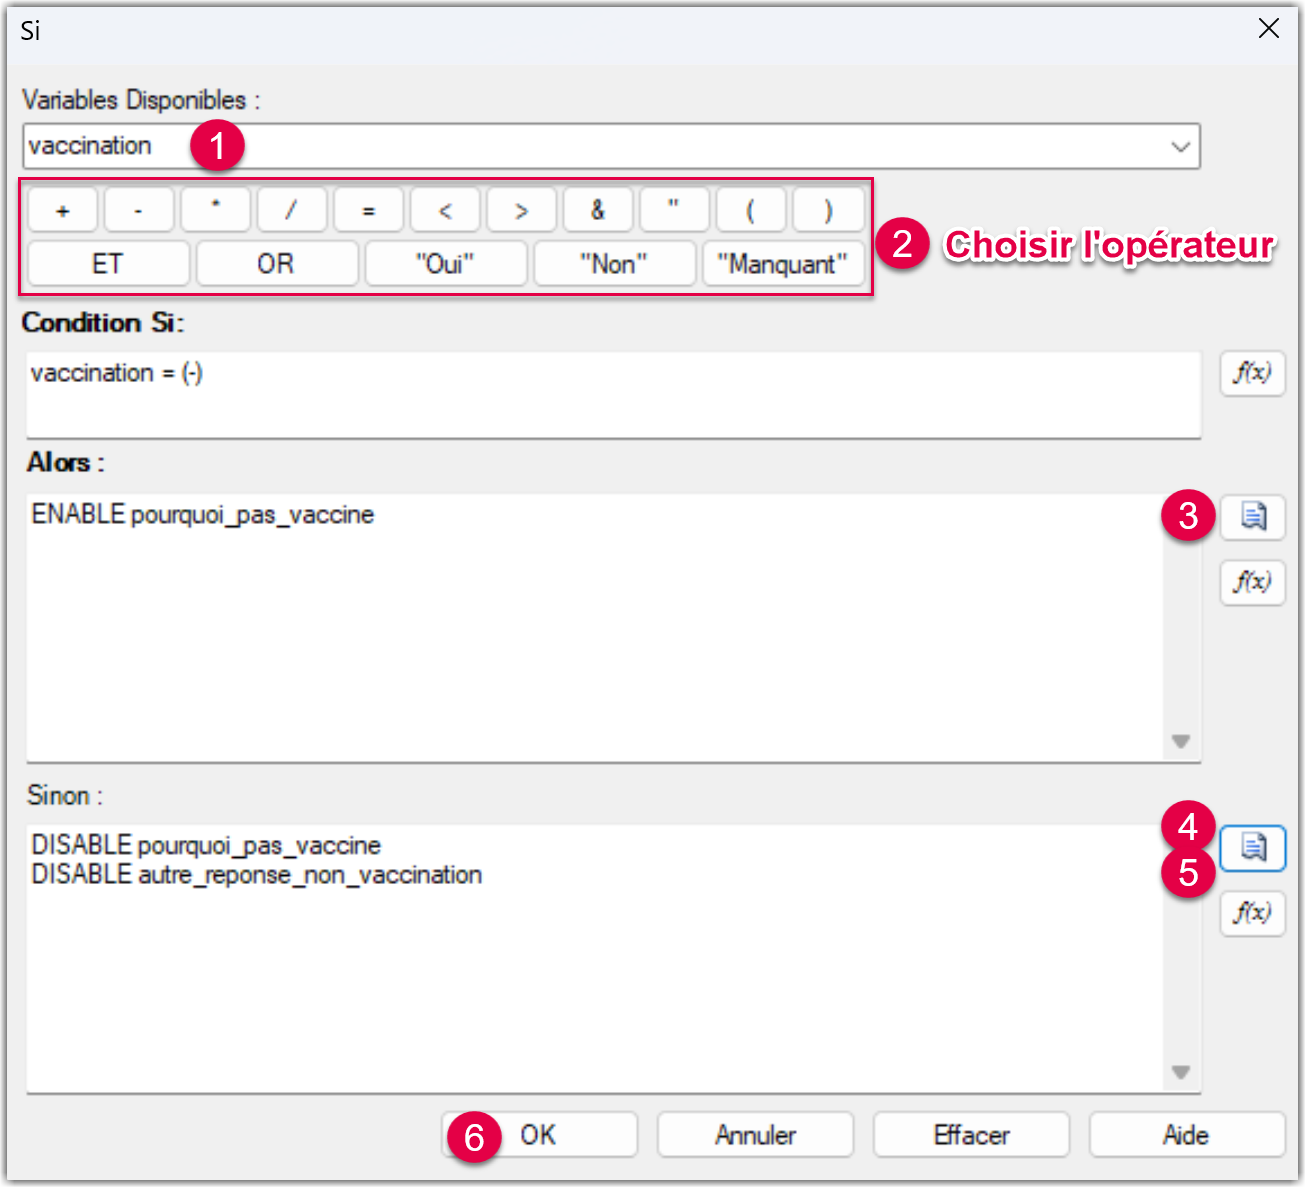
\includegraphics[width=\linewidth,height=0.4\textheight,keepaspectratio]{img/CodeValidation/codeIfEnableDisable}
	\caption{Création de code avec les commandes If, Enable et Disable}
	\label{fig:codeifenabledisable}
\end{figure}

Nous procédons de la même façon pour la variable \var{pourquoi\_pas\_vaccine} (\autoref{fig:codesipasvaccine}). Les codes obtenus s'affichent dans l'éditeur de programme (\autoref{lst:if}, page~\pageref{lst:if}, et \autoref{lst:ifelse}, page~\pageref{lst:ifelse}).

\begin{tcolorbox}[drop lifted shadow]
\begin{lstlisting}[language=EPIscript, style=mystyle, caption={Code de contrôle de la variable vaccination}, label=lst:if]
Field vaccination
	After
		//add code here
		IF vaccination = (-) THEN
			ENABLE pourquoi_pas_vaccine
		ELSE
			DISABLE pourquoi_pas_vaccine
			DISABLE autre_reponse_non_vaccination
		END-IF
	End-After
End-Field
\end{lstlisting}
\end{tcolorbox}

\begin{mybox}[colbacktitle=NOTE]{\faInfoCircle{} À RETENIR}
Dans le code de contrôle, la réponse \kw{Oui} d'un champ Oui/Non s'écrit \commande{(+)} et la réponse \kw{Non} s'écrit \commande{(-)}. Les boutons \kw{"Oui"} et \kw{"Non"} de la fenêtre \kw{Si} les insèrent automatiquement. La condition \commande{vaccination = (-)} signifie donc : \og si la personne n'est pas vaccinée \fg{}.
\end{mybox}

\begin{figure}[H]
	\centering
	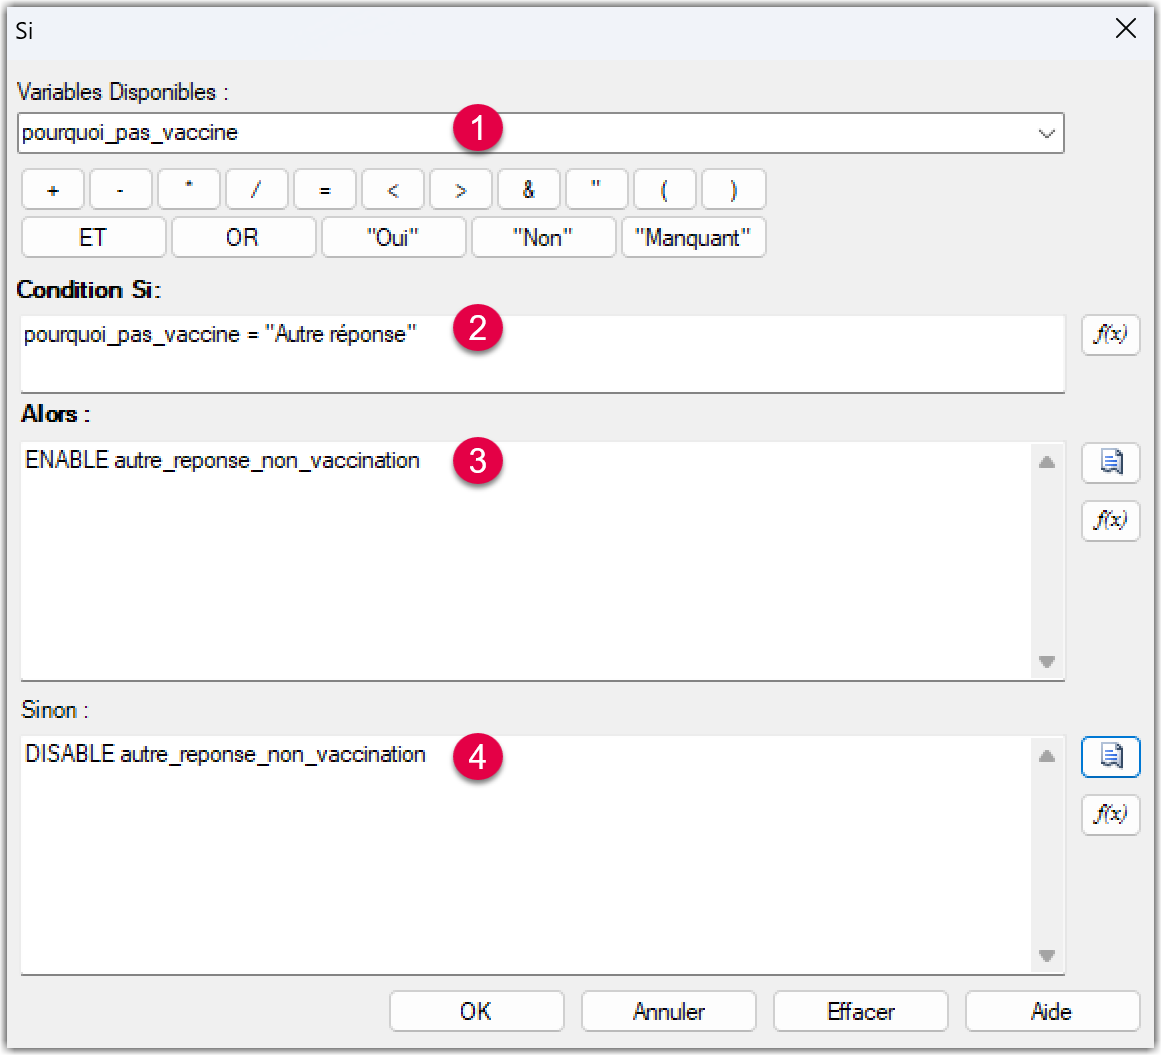
\includegraphics[width=\linewidth,height=0.4\textheight,keepaspectratio]{img/CodeValidation/codeSiPasVaccine}
	\caption{Activer le champ autre\_reponse\_non\_vaccination}
	\label{fig:codesipasvaccine}
\end{figure}

\begin{tcolorbox}[drop lifted shadow]
	\begin{lstlisting}[language=EPIscript, style=mystyle, caption={Code de contrôle de la variable pourquoi\_pas\_vaccine}, label=lst:ifelse]
Field pourquoi_pas_vaccine
	After
		//add code here
		IF pourquoi_pas_vaccine = "Autre réponse" THEN
			ENABLE autre_reponse_non_vaccination
		ELSE
			DISABLE autre_reponse_non_vaccination
		END-IF
	End-After
End-Field
	\end{lstlisting}
\end{tcolorbox}

\begin{mybox}[colbacktitle=CAUTION]{\faFire{} AVERTISSEMENT}
N'oubliez pas les guillemets droits \textcolor{IMPORTANT}{\texttt{"\,"}} pour délimiter une chaîne de caractères (du texte brut, par opposition à un nom de variable) lorsque vous faites une comparaison, comme dans \commande{IF pourquoi\_pas\_vaccine = "Autre réponse"}. Le texte doit être écrit exactement comme dans la liste des valeurs légales, accents et majuscules compris.
\end{mybox}

Comme vous pouvez le constater, le code de contrôle est un outil puissant. Il rend le questionnaire plus robuste et réduit les erreurs de saisie. Son apprentissage peut sembler rebutant au début, mais sa maîtrise vous ouvrira de nombreuses possibilités. Il n'est pas indispensable à la création d'un questionnaire, mais nous vous le recommandons vivement.

\chapter{Saisir des données}
\label{saisirDonnees}
%\minitoc

Lorsque le questionnaire est prêt, et avant de commencer la collecte des vraies données, nous devons le tester pour nous assurer qu'il se comporte comme prévu. Cette étape ne doit pas être négligée : si vous commencez la collecte et découvrez plus tard un problème dans un champ, sa correction peut vous faire perdre les données déjà saisies.

\section{Ouvrir un formulaire pour la saisie}

Pour saisir des données :
\begin{enumerate}
	\item Ouvrir le module \module{saisir des données} d'Epi Info 7 ;
	\item Cliquer sur \kw{Ouvrir le Formulaire} dans la barre d'outils (ou dans le menu \kw{Fichier}). La fenêtre \kw{Ouvrir le Formulaire} s'ouvre (\autoref{fig:ouvrirformulaire}) ;
	\item Dans \kw{Projet en Cours}, cliquer sur \kw{Parcourir} et sélectionner notre projet, le fichier \var{COVID19.prj} ;
	\item Dans la liste \kw{Formulaires}, sélectionner \var{Formulaire1} et valider par \kw{OK} ;
	\item À la première ouverture, une seconde fenêtre intitulée \kw{Propriétés de la table de données} apparaît, avec le nom de la table de données, ici \var{Formulaire1}, et l'identifiant de départ, \kw{1}. Cliquer sur \kw{OK}.
\end{enumerate}

\begin{figure}[H]
	\centering
	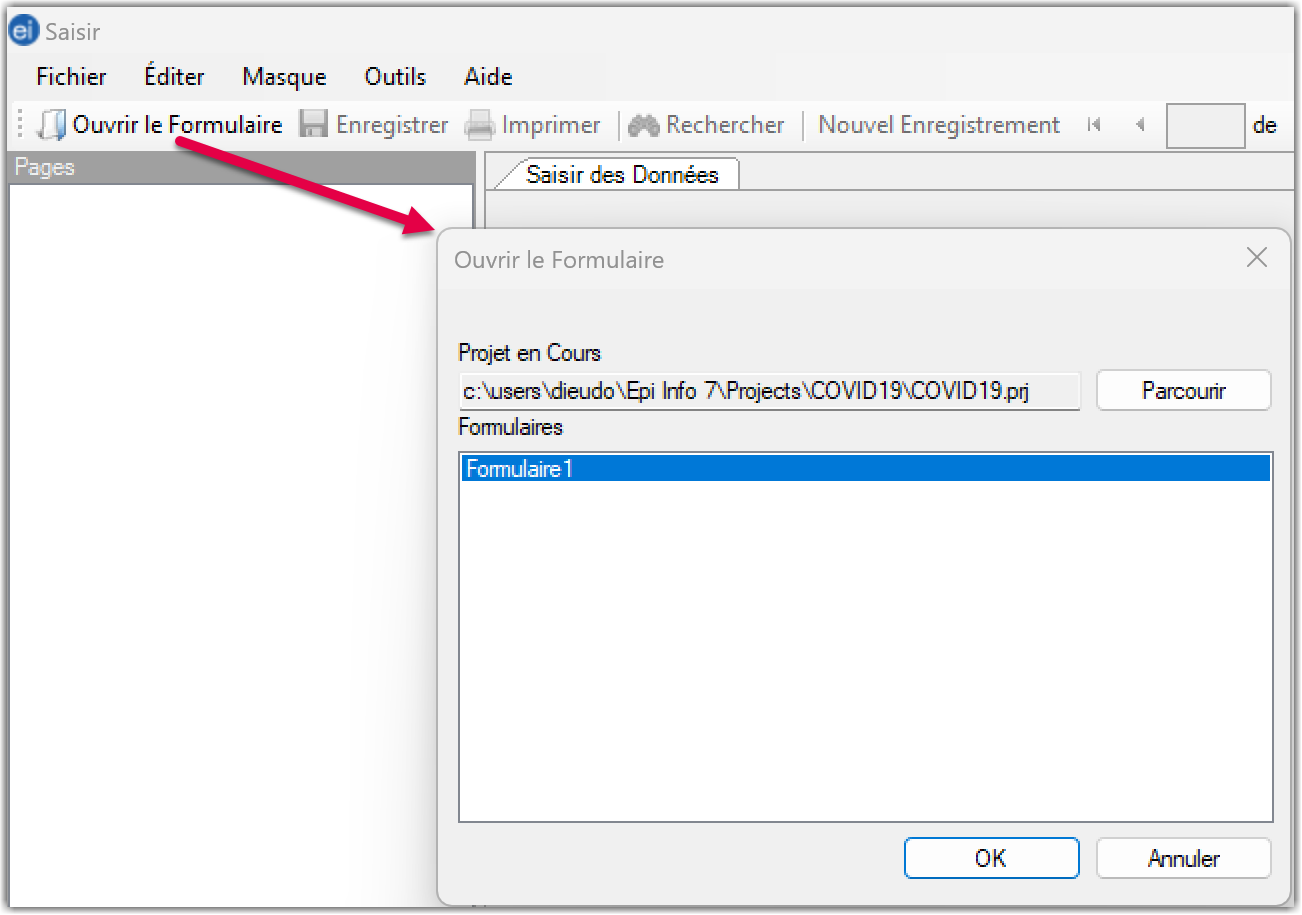
\includegraphics[width=\linewidth,height=0.4\textheight,keepaspectratio]{img/saisirDonnees/ouvrirFormulaire}
	\caption{Ouvrir un formulaire dans le module Saisir des données}
	\label{fig:ouvrirformulaire}
\end{figure}

\begin{mybox}[colbacktitle=TIP]{\faLightbulb{} CONSEIL}
Vous pouvez passer du module \module{créer questionnaires} au module \module{saisir des données} sans quitter l'un pour ouvrir l'autre : cliquez sur \kw{Saisir des données} dans le premier, et sur \kw{Éditer le formulaire} dans le second.
\end{mybox}

\section{Saisir et enregistrer un enregistrement}

Le formulaire s'affiche tel que nous l'avons conçu, avec un enregistrement vide. Pour le remplir :

\begin{enumerate}
	\item Saisir la réponse dans le premier champ, puis appuyer sur la touche \kw{Tabulation} (ou \kw{Entrée}) pour passer au champ suivant, dans l'ordre de tabulation défini au chapitre~\ref{creerQuestionnaire} ;
	\item Observer au passage le comportement du code de contrôle : l'âge et l'IMC doivent se calculer seuls, une taille de 350~cm doit déclencher le message d'alerte, et les questions sur la non-vaccination ne doivent s'activer que si la personne n'est pas vaccinée ;
	\item Pour changer de page, utiliser la liste des pages dans le volet de gauche ;
	\item Une fois tous les champs remplis, cliquer sur \kw{Nouvel enregistrement} pour passer à la fiche suivante.
\end{enumerate}

Epi Info enregistre automatiquement la fiche lorsque l'on passe à un nouvel enregistrement, que l'on change d'enregistrement ou que l'on ferme le formulaire. Le bouton \kw{Enregistrer} permet aussi de sauvegarder à tout moment. Si un champ requis est vide, Epi Info empêche l'enregistrement de la fiche et le signale.

\section{Naviguer et rechercher dans les enregistrements}

La barre d'outils du module permet de se déplacer d'un enregistrement à l'autre : premier, précédent, suivant, dernier. On peut aussi taper directement le numéro de la fiche recherchée. Le bouton \kw{Rechercher} permet de retrouver une fiche à partir de la valeur d'un ou de plusieurs champs, par exemple le nom de la personne enquêtée.

Pour supprimer une fiche saisie par erreur, l'afficher puis cliquer sur \kw{Supprimer}. La fiche est alors marquée comme supprimée et n'est plus prise en compte dans les analyses ; le bouton \kw{Restaurer} permet d'annuler cette suppression.

\section{Tester le questionnaire puis le réinitialiser}

Pour le test, nous saisissons quelques fiches avec des données fictives, en essayant volontairement des valeurs erronées pour vérifier que les contrôles fonctionnent. Si le test est concluant, il faut réinitialiser le questionnaire afin de commencer la collecte avec une table vide. Pour cela, dans le module \module{créer questionnaires}, cliquer sur le menu \kw{Outils} puis sur \kw{Supprimer la table de données}. La procédure est la même si le test révèle des incohérences à corriger dans le questionnaire.

\begin{mybox}[colbacktitle=IMPORTANT]{\faExclamationCircle{} IMPORTANT}
Une fois des données saisies, certaines modifications du questionnaire (supprimer un champ, changer son type ou son nom) ne sont plus possibles ou font perdre les données correspondantes. Pour modifier en profondeur le questionnaire après le test, supprimez d'abord la table de données. Une fois la collecte commencée, évitez de modifier la structure du questionnaire.
\end{mybox}

\chapter{Module Tableau de bord visuel}
\label{moduleTableauDeBord}
%\minitoc

Le \module{tableau de bord visuel} est l'un des deux modules d'analyse d'Epi Info 7. Il est conçu pour être intuitif et simple d'utilisation : grâce aux \emph{gadgets}, il n'est presque pas nécessaire d'écrire du code. Les gadgets permettent de sélectionner, trier, lister ou transformer les données, de réaliser des statistiques simples (fréquences, moyennes, etc.) et des analyses plus avancées (des modèles de régression par exemple). Le module dispose aussi de fonctions graphiques pour visualiser les données. Nous pourrons également représenter nos résultats avec d'autres logiciels comme Microsoft Excel ou LibreOffice Calc, l'équivalent gratuit et multiplateforme d'Excel.

On accède au module à partir de la fenêtre d'accueil d'Epi Info 7, en cliquant sur le bouton \module{tableau de bord visuel} (\autoref{fig:tableaudebord}).

\begin{figure}[H]
	\centering
	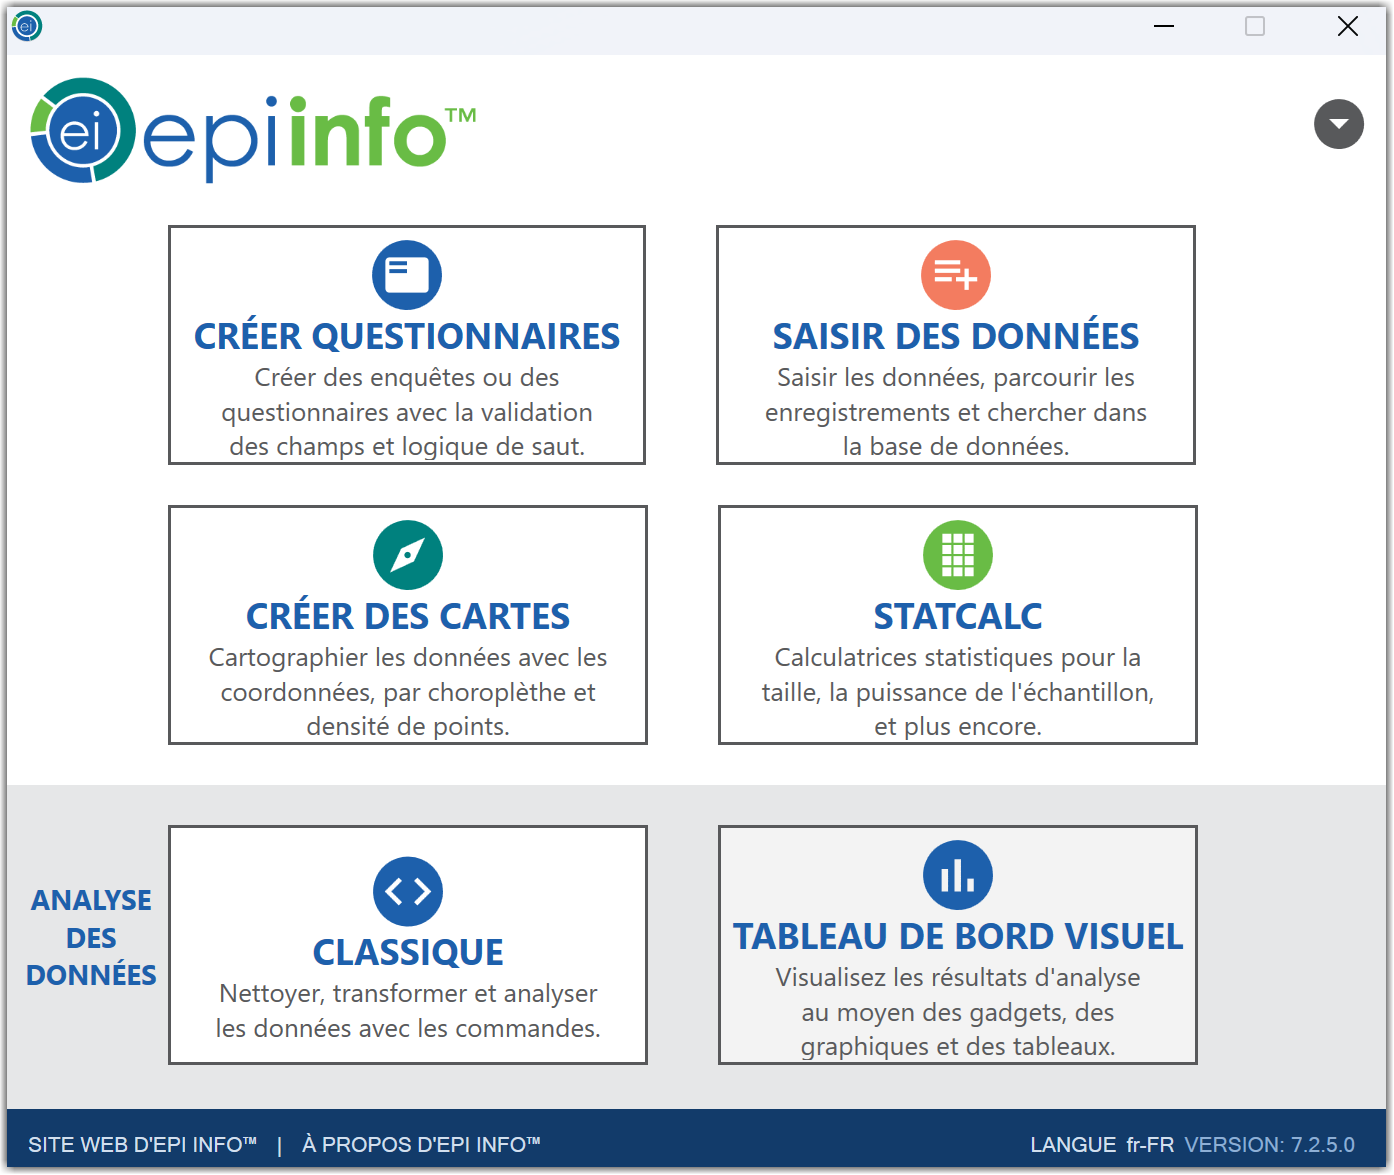
\includegraphics[width=\linewidth,height=0.4\textheight,keepaspectratio]{img/tableauDeBord/tableauDeBord}
	\caption{Le bouton d'ouverture du module Tableau de bord visuel}
	\label{fig:tableaudebord}
\end{figure}

\section{Rappel : les types de variables}
\label{typesVariables}

Avant d'analyser des données, il faut connaître le type de chaque variable, car c'est lui qui détermine les statistiques possibles. On distingue deux grands groupes de variables : les variables \terme{quantitatives} et les variables \terme{qualitatives}.

\subsection{Variables quantitatives}
Les modalités d'une variable quantitative sont des nombres qui expriment une quantité : additionner ou soustraire ces valeurs a un sens. On distingue :

\begin{itemize}
	\item \textbf{les variables quantitatives discrètes}, qui ne prennent que des valeurs isolées, le plus souvent entières, issues d'un comptage (exemple : le nombre d'enfants d'une femme, le nombre de consultations dans l'année) ;
	\item \textbf{les variables quantitatives continues}, qui peuvent prendre n'importe quelle valeur dans un intervalle, issues d'une mesure (exemple : la taille, le poids ou la pression artérielle d'un individu).
\end{itemize}

\subsection{Variables qualitatives}
Les modalités d'une variable qualitative ne sont pas des quantités numériques : on ne peut pas en faire la somme ou la différence. Le groupe sanguin du système ABO, avec ses modalités A, B, AB et O, en est un exemple. Une variable qualitative peut être :

\begin{itemize}
	\item \textbf{binaire} : elle n'a que deux modalités. Exemples : le sexe (masculin/féminin), être au chômage (oui/non), être majeur (oui/non). Les variables binaires sont très utilisées, notamment en épidémiologie (malade/non malade, exposé/non exposé) ;
	\item \textbf{ordinale} : ses modalités sont ordonnées. Exemple : le niveau de satisfaction vis-à-vis d'un service de santé, avec les modalités \og pas du tout satisfait \fg{}, \og peu satisfait \fg{}, \og moyennement satisfait \fg{} et \og très satisfait \fg{}, que l'on peut coder 0, 1, 2 et 3 ;
	\item \textbf{nominale} : elle a trois modalités ou plus, sans ordre entre elles. Exemples : la couleur des yeux, la profession, le groupe sanguin.
\end{itemize}

\section{Ouvrir le module et importer des données}

Comme de nombreux logiciels d'analyse statistique (\textsc{r}, \textsc{stata}, \textsc{spss}\ldots), Epi Info 7 est fourni avec des bases de données d'exemple pour apprendre les statistiques. Pour que chacun puisse refaire les manipulations, nous utiliserons dans ce chapitre la base \var{EColi}, qui décrit une épidémie d'infection à \emph{Escherichia coli} liée à l'alimentation.

Lorsque nous ouvrons le module \module{tableau de bord visuel}, son interface présente trois parties principales : l'\kw{en-tête}, le \kw{canevas} et la \kw{barre d'état} (\autoref{fig:interfacetableaubord}).

\begin{figure}[H]
	\centering
	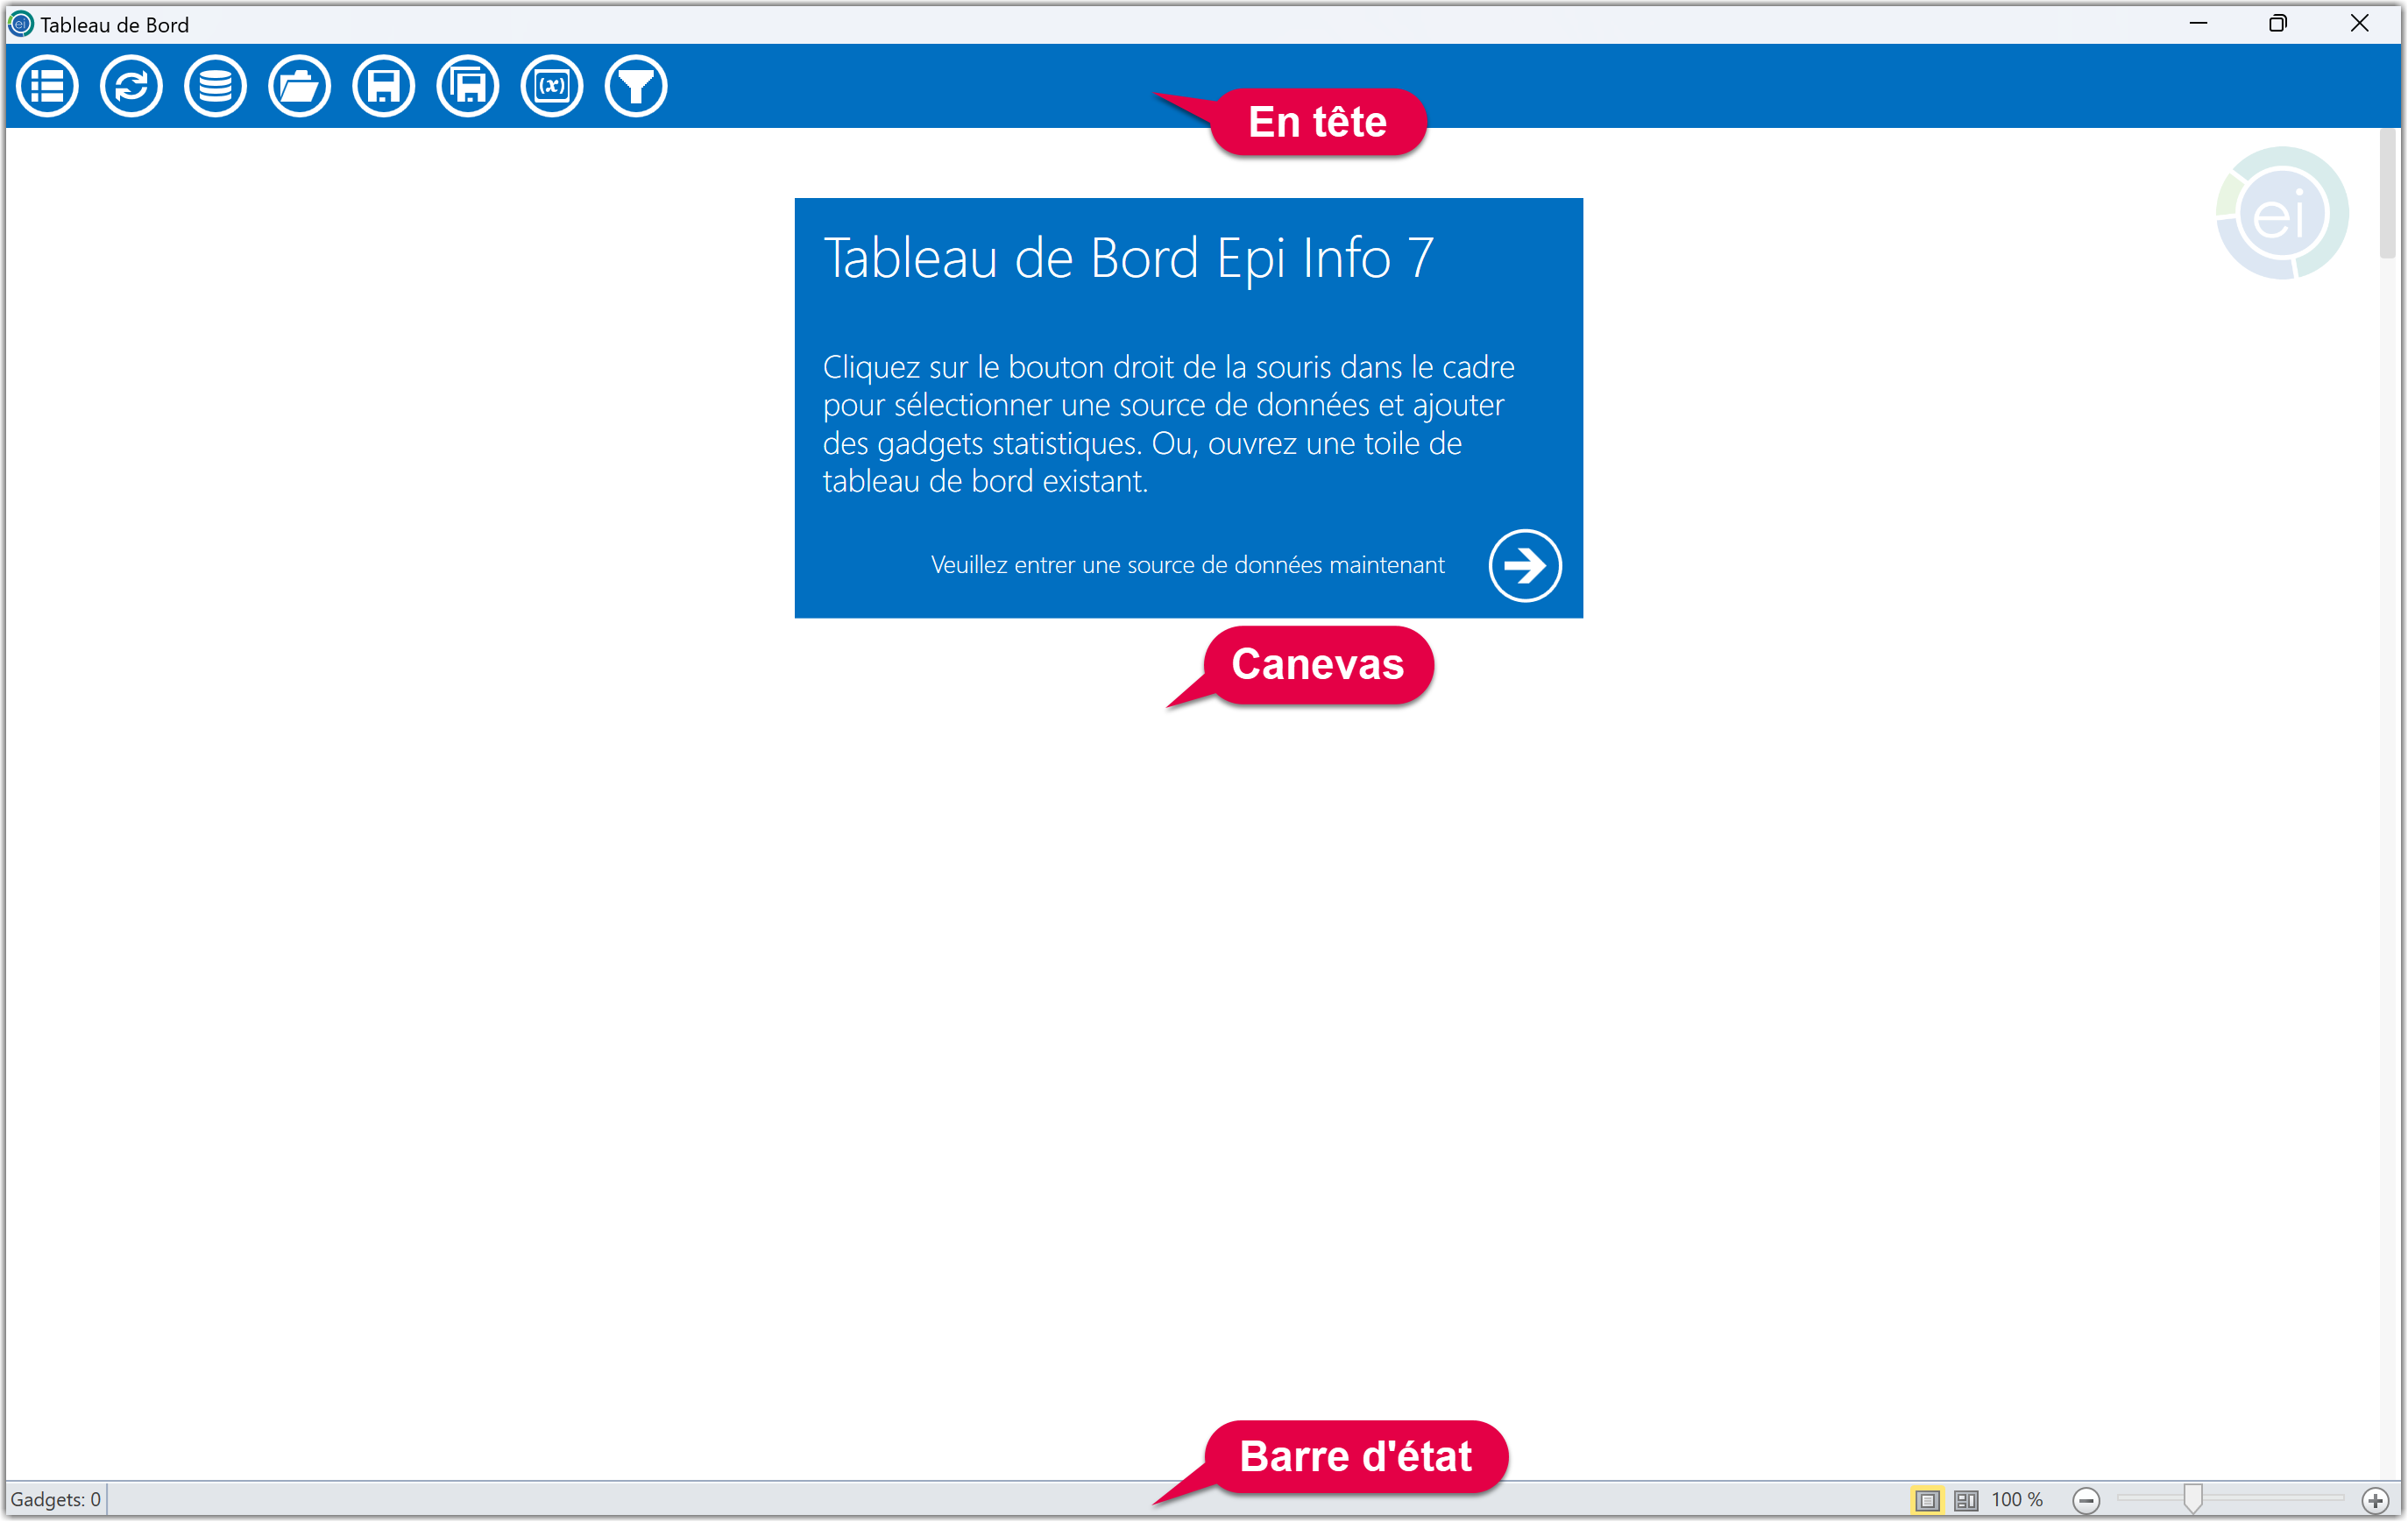
\includegraphics[width=\linewidth,height=0.4\textheight,keepaspectratio]{img/tableauDeBord/interfaceTableauBord}
	\caption{Interface du module Tableau de bord visuel}
	\label{fig:interfacetableaubord}
\end{figure}

Pour importer les données d'une base Epi Info 7, procéder comme suit (\autoref{fig:importerbaseepi}) :
\begin{itemize}
	\item Cliquer sur \kw{Veuillez entrer une source de données maintenant} dans le canevas, ou sur le symbole de base de données dans l'en-tête ;
	\item Cliquer sur le bouton \kw{Parcourir}. Une fenêtre s'ouvre sur le dossier \var{Projects} d'Epi Info, qui contient toutes les bases fournies avec le logiciel ;
	\item Choisir la base de données \var{EColi} ;
	\item La base comporte deux formulaires : \var{FoodHistory} et \var{FoodHistory\_NoCheckCode}. Sélectionner le premier, \var{FoodHistory} ;
	\item Valider par \kw{OK}.
\end{itemize}

\begin{figure}[H]
	\centering
	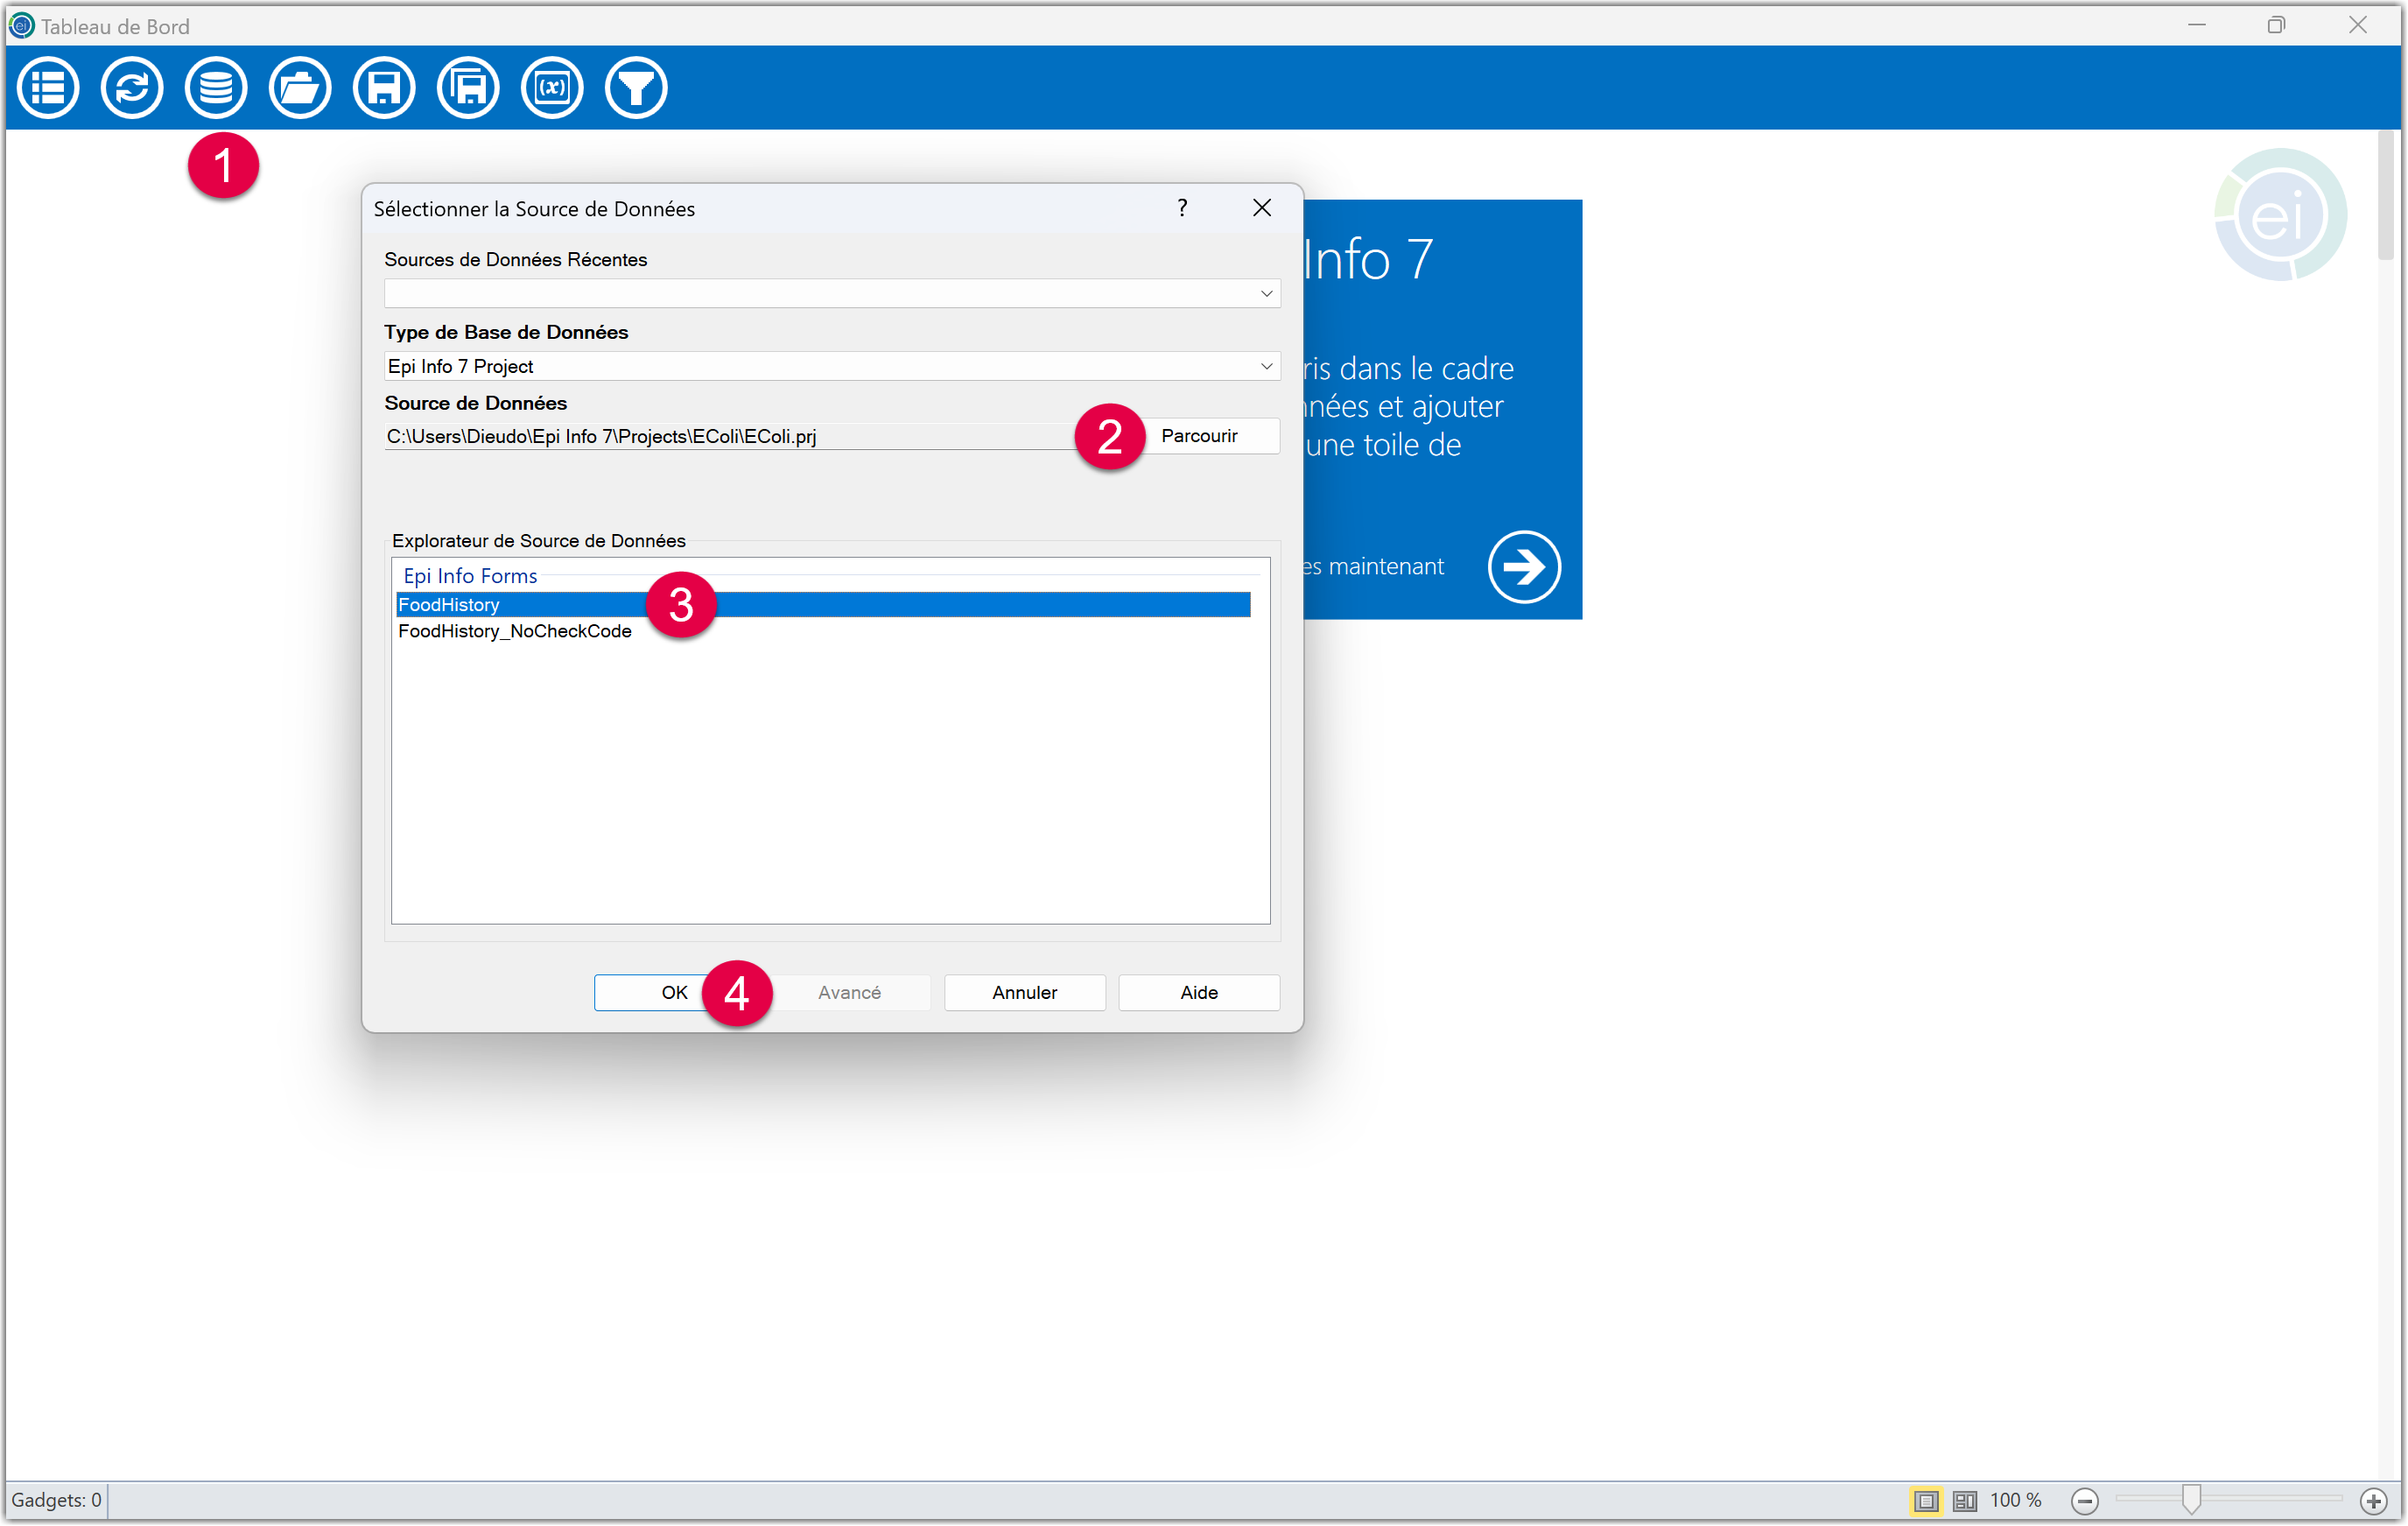
\includegraphics[width=\linewidth,height=0.4\textheight,keepaspectratio]{img/tableauDeBord/importerBaseEpi}
	\caption{Importer une base de données Epi Info 7}
	\label{fig:importerbaseepi}
\end{figure}

Après l'import, le nombre d'enregistrements de la base s'affiche en haut à droite : 359 enregistrements. Ce nombre apparaît aussi dans la barre d'état, avec le nombre de champs, 83. Deux volets apparaissent sur les bords gauche et droit du canevas ; ils se déplient au survol de la souris. Le volet de gauche, \kw{Variables définies}, permet de créer et de recoder des variables ; celui de droite, \kw{Filtres de données}, permet de travailler sur un sous-groupe de données (\autoref{fig:interfaceapresimportdonnees}).

\begin{figure}[H]
	\centering
	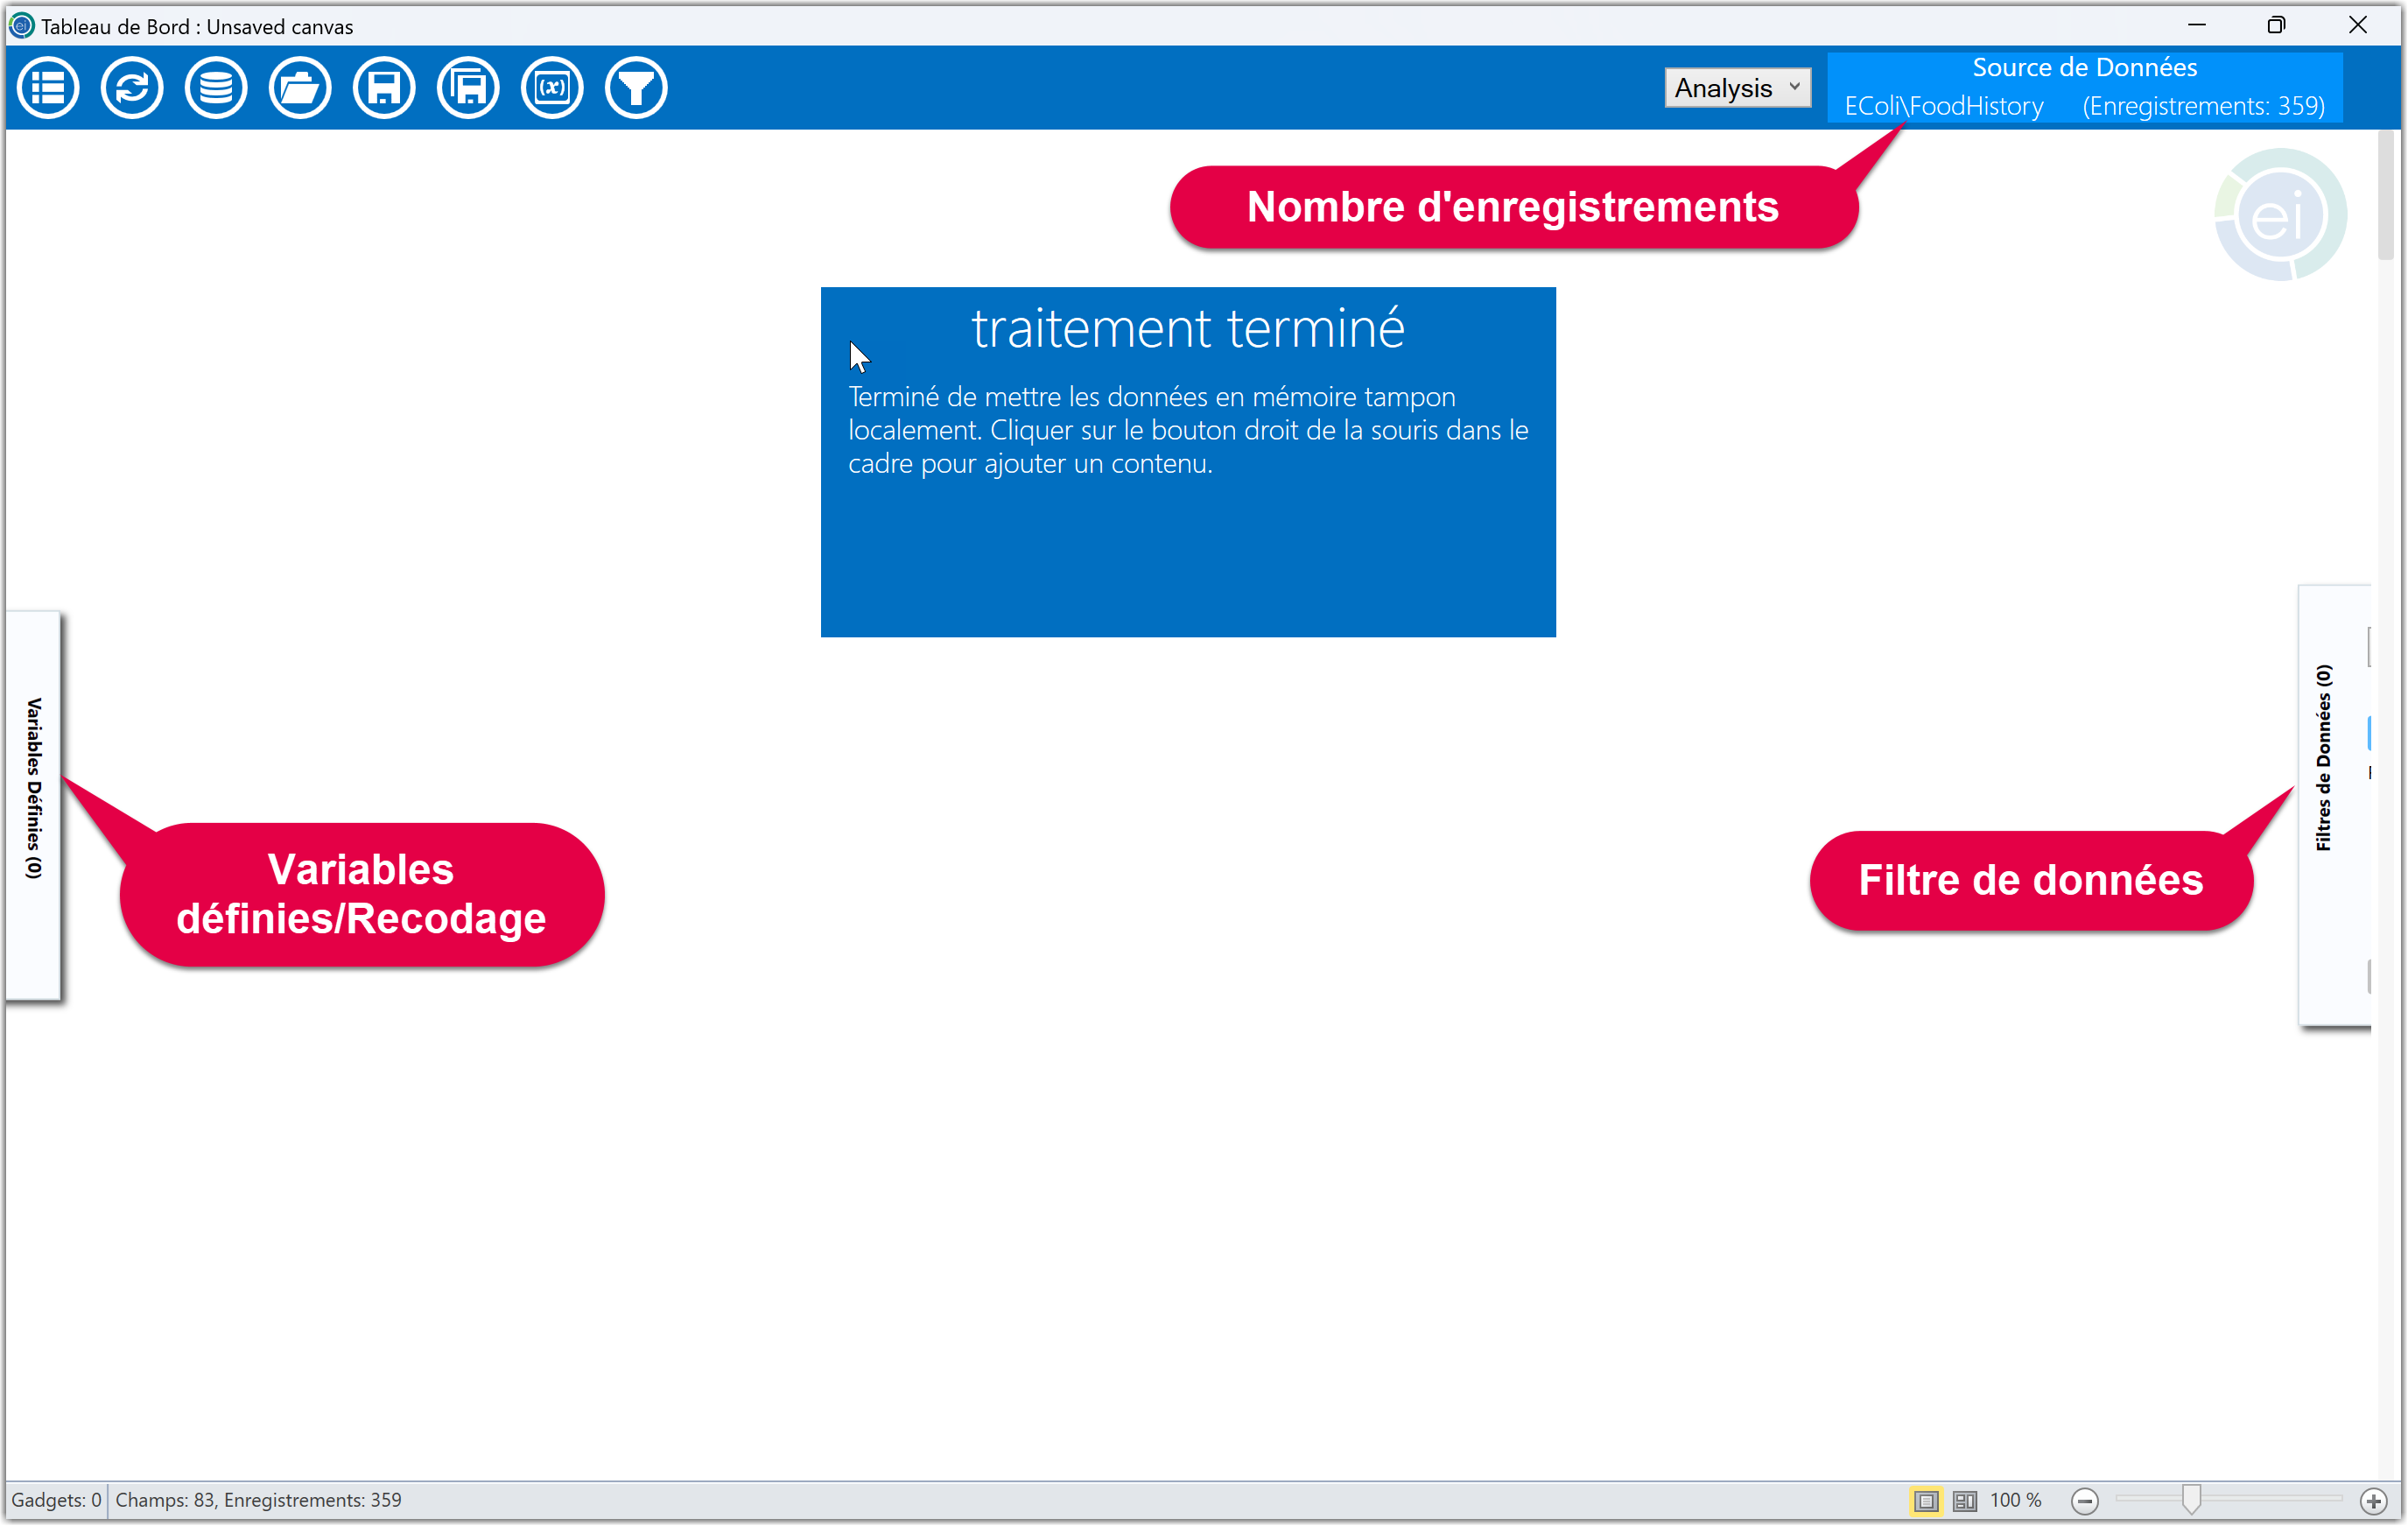
\includegraphics[width=\linewidth,height=0.4\textheight,keepaspectratio]{img/tableauDeBord/interfaceApresImportDonnees}
	\caption{Interface du Tableau de bord après l'import des données}
	\label{fig:interfaceapresimportdonnees}
\end{figure}

\section{Statistiques descriptives}

Passons maintenant à l'analyse statistique proprement dite, en commençant par la statistique descriptive. Nous utiliserons pour cela les gadgets d'analyse.

Pour ajouter un gadget, faire un clic droit sur le canevas puis aller à \kw{Ajouter un gadget d'analyse}, repéré par une roue dentée. Au survol de cette ligne, un sous-menu apparaît avec les différents gadgets : moyennes, fréquences, etc. (\autoref{fig:TBajoutergadget}).

\begin{figure}[H]
	\centering
	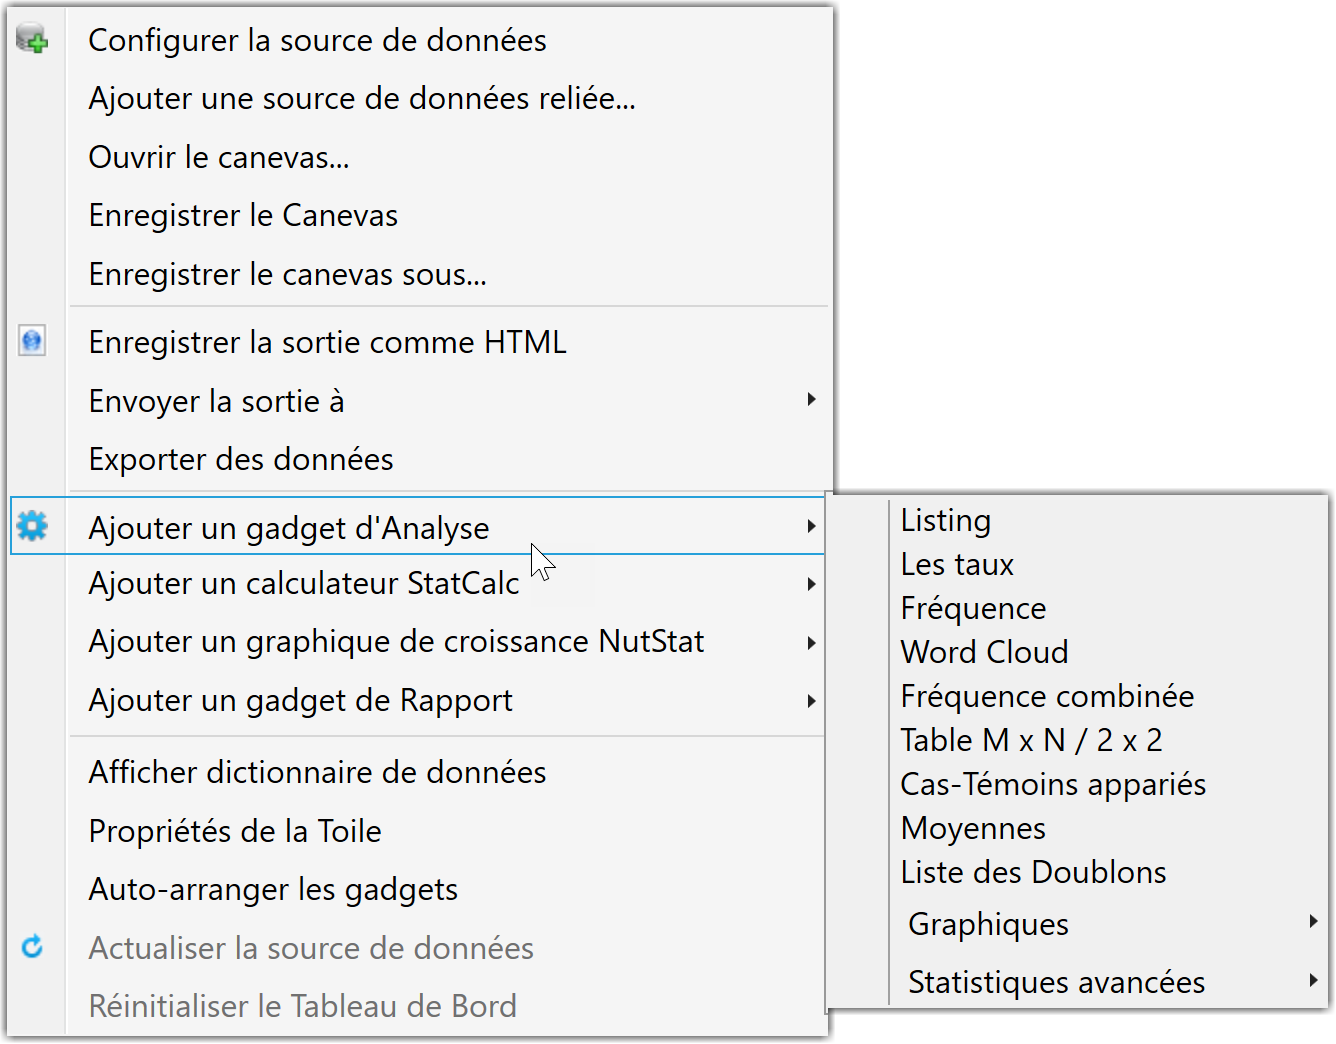
\includegraphics[width=\linewidth,height=0.4\textheight,keepaspectratio]{img/tableauDeBord/ajouterGadget}
	\caption{Ajouter un gadget d'analyse}
	\label{fig:TBajoutergadget}
\end{figure}

Le gadget \kw{Listing} affiche les données brutes des variables choisies. Il permet de jeter un premier coup d'œil aux données et d'exporter les variables sélectionnées au format Excel.

\subsection{Calculer une fréquence}

Le tableau de fréquences est l'outil de base pour décrire une variable qualitative : il donne, pour chaque modalité, l'effectif et le pourcentage. Pour l'obtenir :

\begin{itemize}
	\item Faire un clic droit sur le canevas ;
	\item Aller à \kw{Ajouter un gadget d'analyse} ;
	\item Cliquer sur \kw{Fréquence} dans le sous-menu ;
	\item Dans le champ \kw{Variables}, choisir la variable à décrire, ici \var{ILL} (\og malade \fg{} en anglais) ;
	\item Valider par \kw{OK} (\autoref{fig:frequence}).
\end{itemize}

\begin{figure}[H]
	\centering
	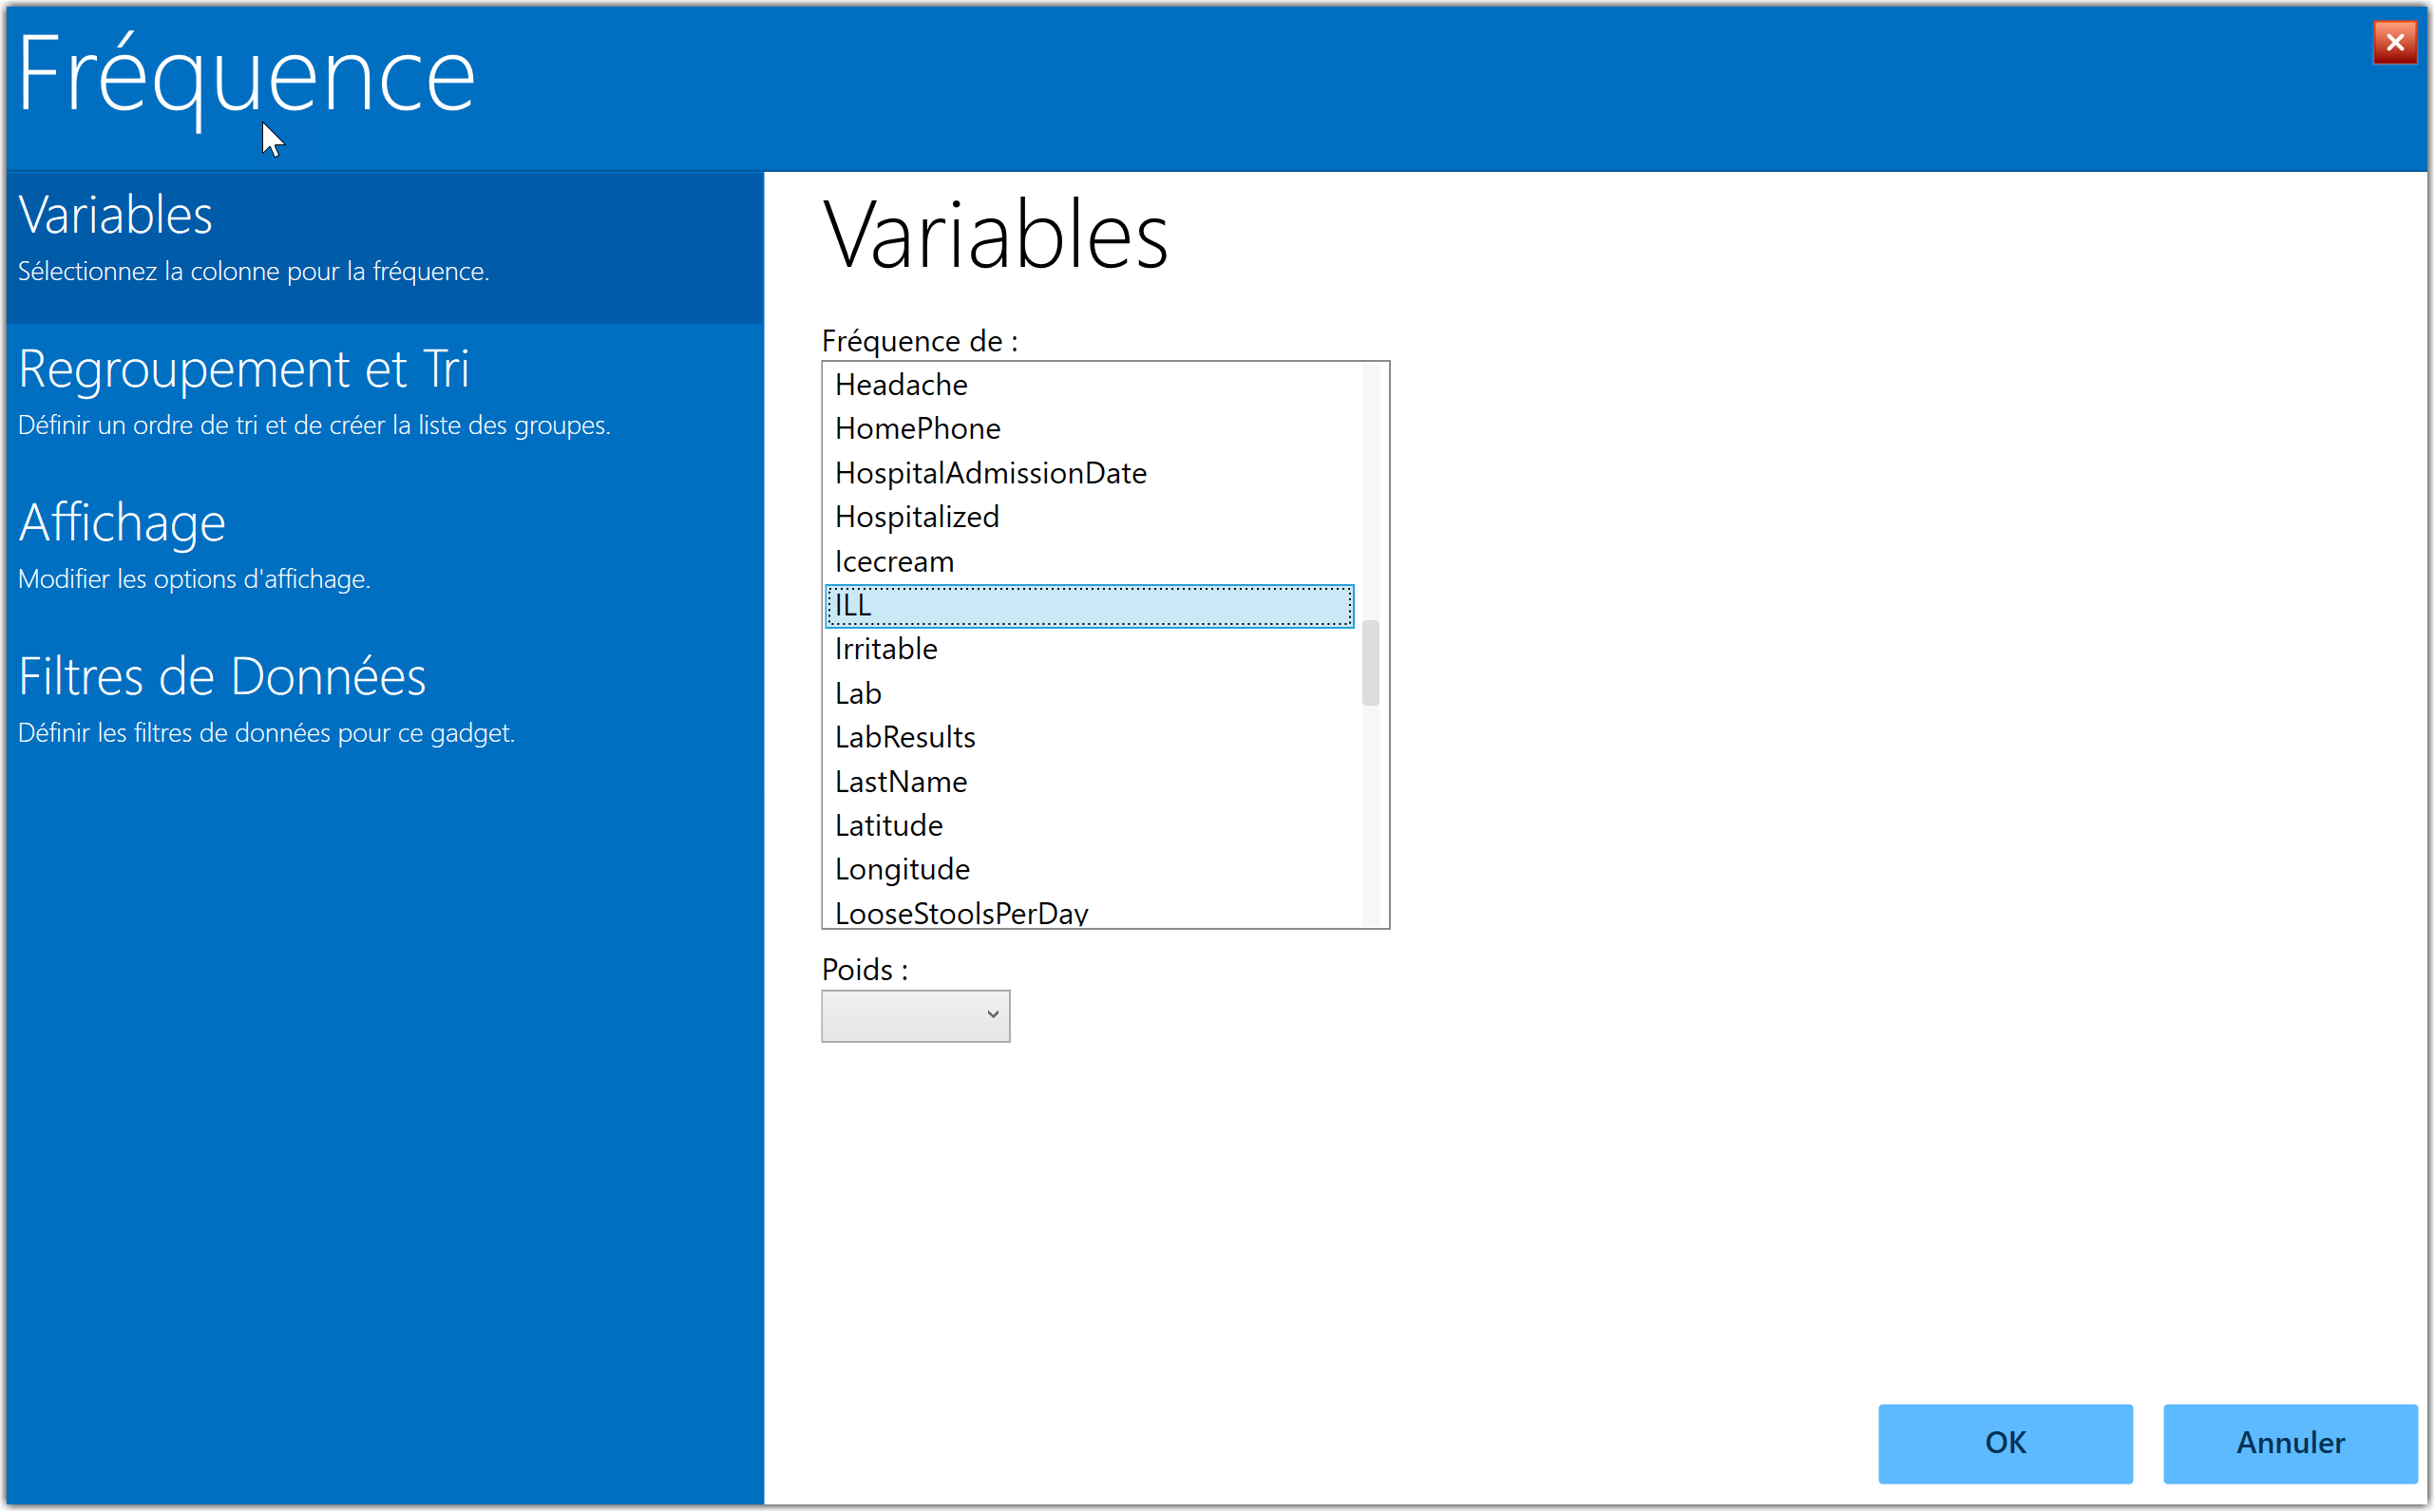
\includegraphics[width=\linewidth,height=0.4\textheight,keepaspectratio]{img/tableauDeBord/frequence}
	\caption{Créer une fréquence}
	\label{fig:frequence}
\end{figure}

Le gadget de fréquence de la variable \var{ILL} s'affiche alors (\autoref{fig:frequenceill}). Sur 359 personnes enquêtées, 276 étaient malades (\kw{Yes}) et 83 ne l'étaient pas (\kw{No}), soit respectivement 76,88~\% et 23,12~\%. Les deux dernières colonnes donnent l'intervalle de confiance à 95~\% de chaque pourcentage, calculé par la méthode de Wilson : par exemple, la proportion de malades est comprise entre 72,25~\% et 80,94~\%.

\begin{figure}[H]
	\centering
	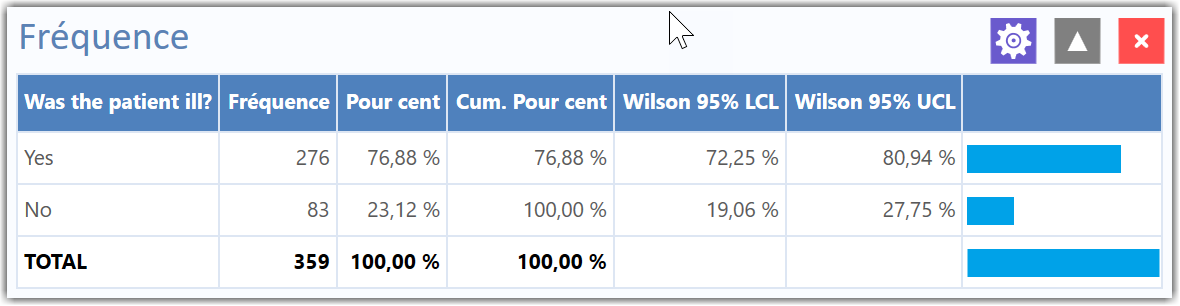
\includegraphics[width=\linewidth,height=0.4\textheight,keepaspectratio]{img/tableauDeBord/frequenceILL}
	\caption{Fréquence de la variable ILL}
	\label{fig:frequenceill}
\end{figure}

Nous pouvons stratifier une fréquence selon une autre variable pour obtenir des informations supplémentaires. Cherchons par exemple la proportion de malades selon le sexe. La variable du sexe s'appelle ici \var{Sex} ; deux de ses modalités contiennent des données : \kw{M-Male} (sexe masculin) et \kw{F-Female} (sexe féminin)\footnote{La variable \var{Sex} compte en réalité six modalités, mais quatre d'entre elles ne contiennent aucune donnée et n'apparaissent donc pas : \kw{A-Ambiguous}, \kw{N-Not applicable}, \kw{O-Other} et \kw{U-Unknown}.}. Pour cela :
\begin{itemize}
	\item Rouvrir les paramètres du gadget de fréquence, soit comme précédemment, soit plus simplement en cliquant sur la roue dentée en haut à droite du gadget (\autoref{fig:frequenceill}) ;
	\item Dans le volet bleu à gauche, aller dans l'onglet \kw{Regroupement et tri} et sélectionner la variable \var{Sex} ;
	\item Valider par \kw{OK}.
\end{itemize}

Nous obtenons deux tableaux (\autoref{fig:frequenceillsex}). Le tableau du haut concerne les femmes, celui du bas les hommes. Sur 186 femmes, 147 (79,03~\%) sont malades et 39 (20,97~\%) ne le sont pas. Sur 173 hommes, 129 (74,57~\%) sont malades et 44 (25,43~\%) ne le sont pas.

\begin{figure}[H]
	\centering
	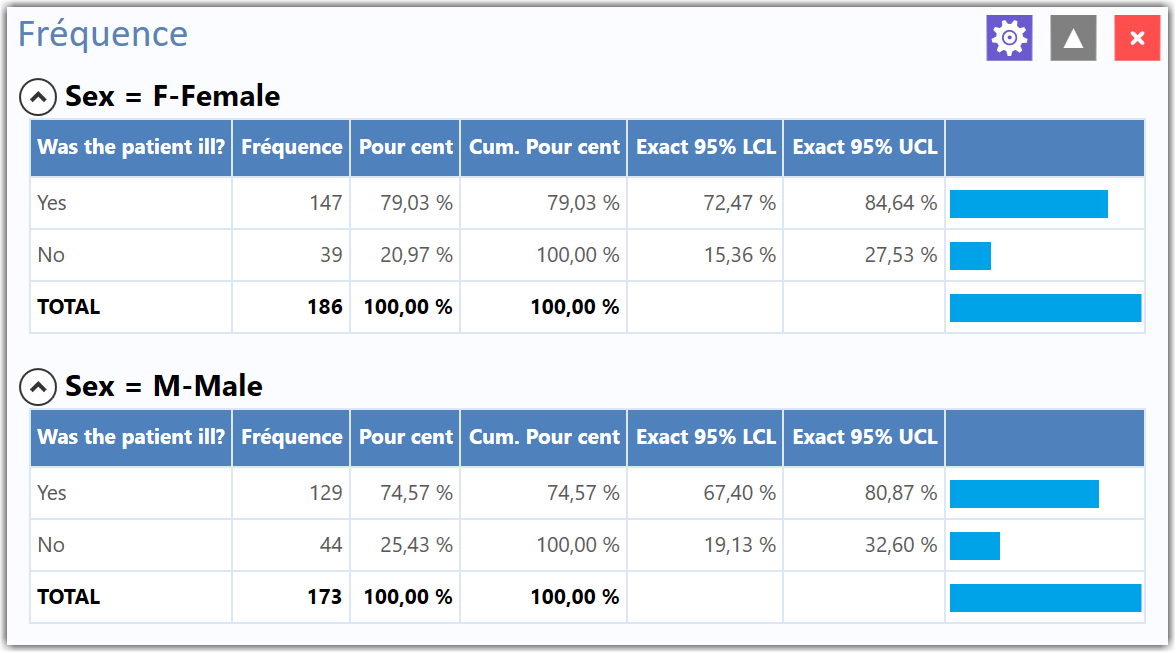
\includegraphics[width=\linewidth,height=0.4\textheight,keepaspectratio]{img/tableauDeBord/frequenceIllSex}
	\caption{Fréquence des malades selon le sexe}
	\label{fig:frequenceillsex}
\end{figure}

\section{Paramètres de position}

Les paramètres de position, ou de tendance centrale, donnent l'ordre de grandeur des mesures : ce sont les valeurs autour desquelles se regroupent les observations de l'échantillon. Ils s'appliquent aux variables quantitatives.

\subsection{La moyenne}
\label{moyenne}
La valeur centrale la plus utilisée est la moyenne arithmétique, notée $\bar{x}$ : c'est la somme des mesures divisée par le nombre de mesures $n$.
\[
\bar{x}=\frac{1}{n} \sum_{i=1}^n x_i
\]

Exemple : soit la taille, en centimètres, de cinq individus : 170, 191, 175, 154 et 182. En appliquant la formule, la taille moyenne est $(170+191+175+154+182)/5 = 872/5 = 174{,}4$~cm.

La moyenne est facile à calculer, mais elle est sensible aux valeurs extrêmes et aux erreurs de saisie : une seule valeur aberrante peut la déplacer fortement.

Calculons maintenant l'âge moyen des personnes de la base EColi :

\begin{itemize}
	\item Faire un clic droit sur le canevas ;
	\item Aller à \kw{Ajouter un gadget d'analyse} ;
	\item Cliquer sur \kw{Moyennes} ;
	\item Vérifier que vous êtes dans l'onglet consacré aux variables ;
	\item Sélectionner la variable \var{Age} ;
	\item Valider par \kw{OK}.
\end{itemize}

Nous obtenons le résultat de la \autoref{fig:moyenne}.

\begin{figure}[H]
	\centering
	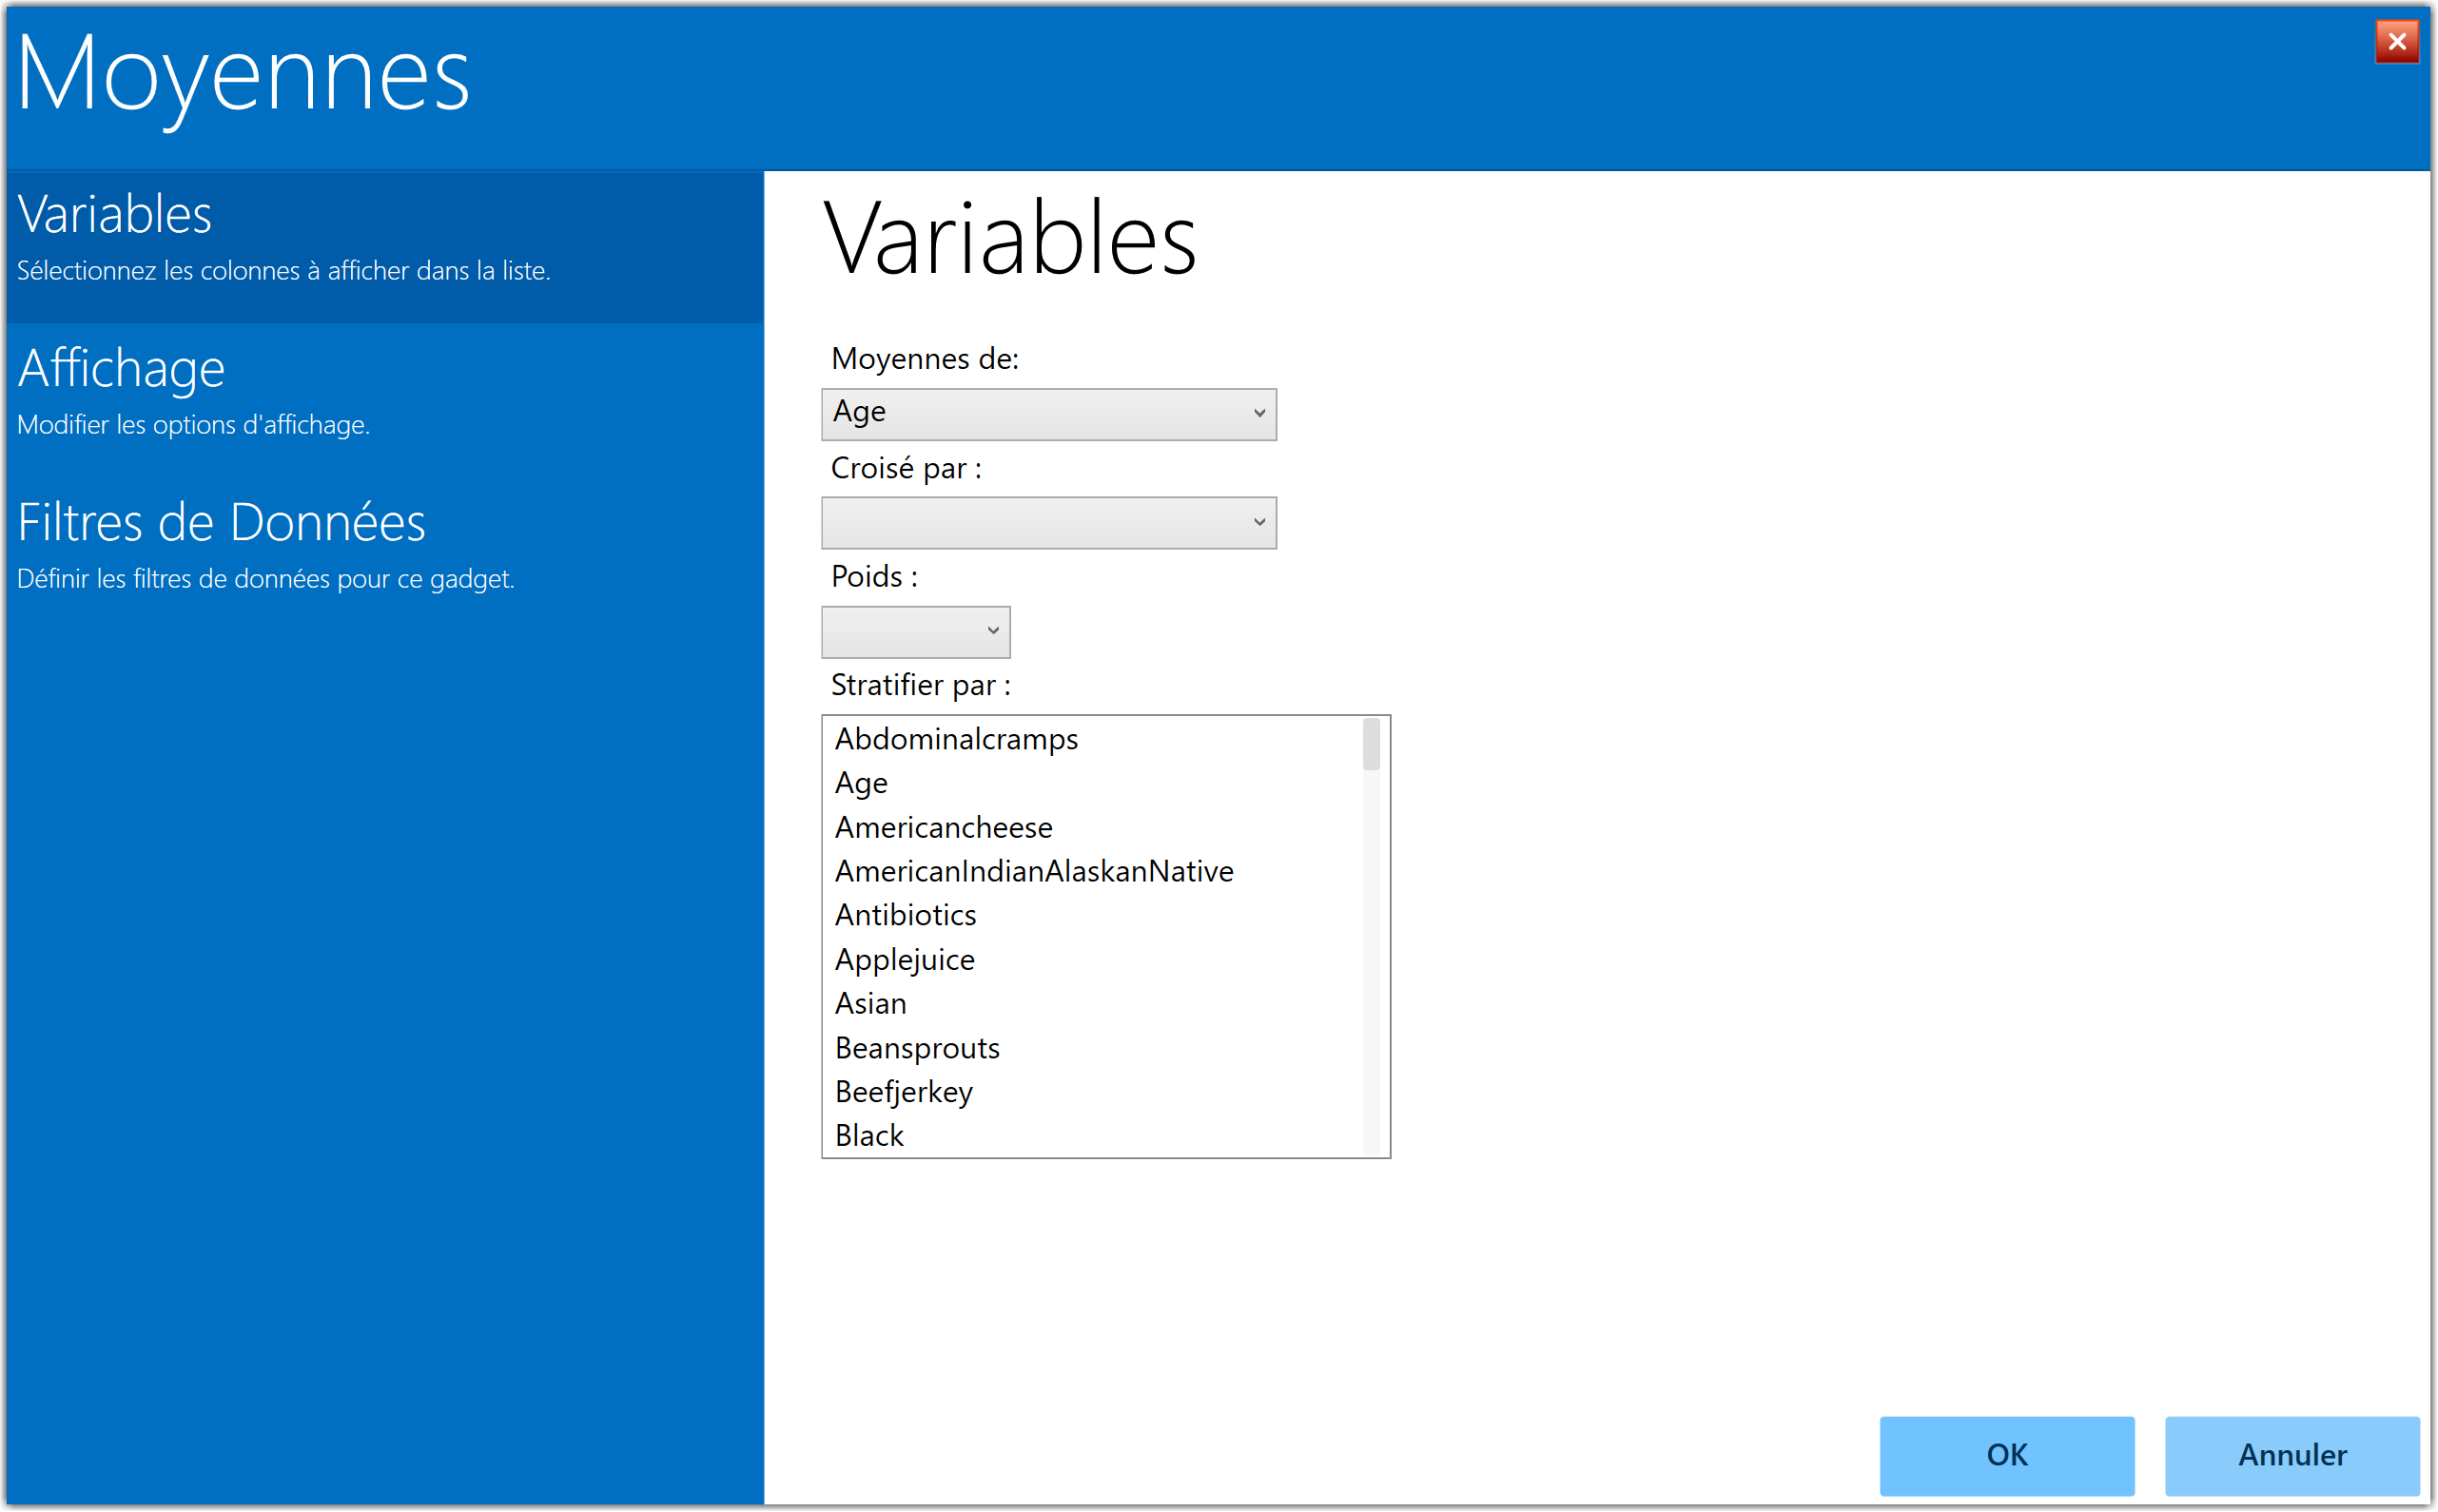
\includegraphics[width=\linewidth,height=0.4\textheight,keepaspectratio]{img/tableauDeBord/moyenne}
	\caption{Calcul de la moyenne des âges}
	\label{fig:moyenne}
\end{figure}

Comme pour la fréquence, nous pouvons croiser la moyenne avec une autre variable. Associons à la variable âge la variable sexe pour connaître l'âge moyen des femmes et celui des hommes :
\begin{itemize}
	\item Rouvrir les paramètres du gadget des moyennes, par exemple en cliquant sur la roue dentée en haut à droite du gadget (\autoref{fig:moyenne}) ;
	\item Rester dans l'onglet consacré aux variables et, dans le champ \kw{Croisé par}, sélectionner la variable \var{Sex} ;
	\item Valider par \kw{OK}.
\end{itemize}

Les résultats s'affichent comme sur la \autoref{fig:moyenneresultatage}. Pour l'ensemble de l'échantillon, ils se lisent ainsi :

\begin{figure}[H]
	\centering
	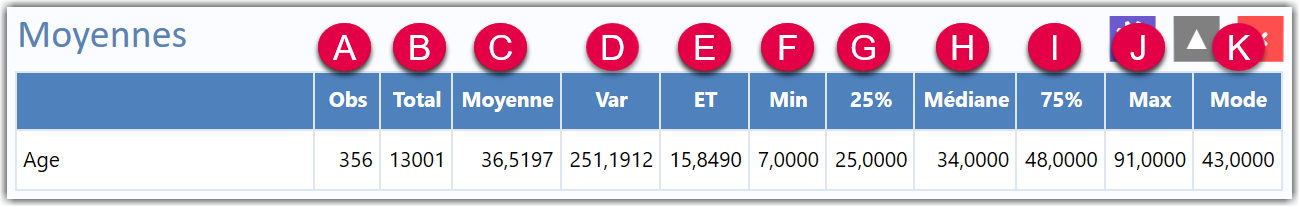
\includegraphics[width=\linewidth,height=0.4\textheight,keepaspectratio]{img/tableauDeBord/moyenneResultatAge}
	\caption{Résultat du calcul de la moyenne des âges}
	\label{fig:moyenneresultatage}
\end{figure}

\begin{description}
	\item[A] \kw{Obs} : le nombre d'observations, égal à 356 ;
	\item[B] \kw{Total} : la somme des âges, égale à 13\,001 ;
	\item[C] \kw{Moyenne} : la \terme{moyenne} des âges, égale au rapport $B/A$, soit $13\,001/356 = 36{,}52$ ans ;
	\item[D] \kw{Var} : la \terme{variance}, égale à 251,19 ;
	\item[E] \kw{ET} : l'\terme{écart-type}, égal à 15,85 ans ;
	\item[F] \kw{Min} : le \terme{minimum}, 7 ans ;
	\item[G] \kw{25\,\%} : le \terme{premier quartile}, 25 ans ;
	\item[H] \kw{Médiane} : la \terme{médiane}, 34 ans ;
	\item[I] \kw{75\,\%} : le \terme{troisième quartile}, 48 ans ;
	\item[J] \kw{Max} : le \terme{maximum}, 91 ans ;
	\item[K] \kw{Mode} : le \terme{mode}, c'est-à-dire l'âge le plus fréquent, 43 ans.
\end{description}

Pas d'inquiétude si certains termes vous sont encore inconnus : nous les expliquons dans les sections suivantes.

\subsection{La médiane}

La médiane est la valeur qui partage la série en deux groupes de même effectif : autant d'observations lui sont inférieures que supérieures. Elle s'exprime dans la même unité que les valeurs observées.
Pour déterminer la médiane d'une série, il faut d'abord l'ordonner. Reprenons l'exemple des cinq tailles. Une fois ordonnée, la série devient : 154, 170, 175, 182, 191. La médiane est la valeur du milieu, soit 175~cm. Lorsque l'effectif est pair, la médiane est la moyenne des deux valeurs du milieu.

Contrairement à la moyenne, la médiane est peu sensible aux valeurs extrêmes. On la préfère donc pour décrire une variable dont la distribution est asymétrique.

\subsection{Le mode}
Le mode, ou valeur dominante, est la valeur de la variable dont la fréquence est la plus élevée.
Lorsque les données sont regroupées en classes, on parle de classe modale : c'est la classe dont la fréquence est maximale. Dans le cas d'une courbe continue des fréquences, c'est l'abscisse du point le plus haut de la courbe.
Lorsque la distribution est symétrique et unimodale, la moyenne, la médiane et le mode sont confondus.

\subsection{Les quantiles}
Les quantiles sont les valeurs qui partagent l'échantillon ordonné en groupes de même effectif. Ils portent des noms différents selon le nombre de groupes : quartiles pour quatre groupes, déciles pour dix groupes, centiles pour cent groupes.

Pour partager la série en quatre groupes de même effectif, il faut trois valeurs, appelées quartiles : $Q_1$, $Q_2$ et $Q_3$. Un quart des observations se trouve entre le minimum et $Q_1$, un quart entre $Q_1$ et $Q_2$, un quart entre $Q_2$ et $Q_3$, et le dernier quart entre $Q_3$ et le maximum. Comme nous le verrons dans la section sur les paramètres de dispersion, les quartiles servent aussi à définir des intervalles.

\begin{mybox}[colbacktitle=NOTE]{\faInfoCircle{} À RETENIR}
Le deuxième quartile, $Q_2$, n'est autre que la médiane.
\end{mybox}

\section{Paramètres de dispersion}
Deux séries peuvent avoir la même moyenne tout en étant très différentes : l'une très resserrée autour de la moyenne, l'autre très étalée. Les paramètres de dispersion mesurent cet étalement.

\subsection{Variance et écart-type}
La variance est la moyenne des carrés des écarts à la moyenne de l'échantillon :
\[
\operatorname{Var}(X)=\frac{1}{n}\sum_{i=1}^n \left(x_i-\bar{x}\right)^2
\]
où $\bar{x}$ est la moyenne de la série et $n$ l'effectif.

\begin{mybox}[colbacktitle=CAUTION]{\faFire{} AVERTISSEMENT}
$\operatorname{Var}(X)$ est la variance de l'échantillon : ce n'est ni la variance de la population dont l'échantillon est issu, ni une estimation de celle-ci. Pour estimer la variance de la population, on divise par $n-1$ au lieu de $n$. C'est cette variance estimée que calculent la plupart des logiciels, dont Epi Info.
\end{mybox}

La variance s'exprime dans le carré de l'unité de mesure (en années$^2$ pour l'âge), ce qui la rend difficile à interpréter. Pour disposer d'un indice de dispersion exprimé dans la même unité que la variable, on utilise sa racine carrée, l'écart-type :
\[
\text{Écart-type}(X)=\sqrt{\operatorname{Var}(X)}
\]
Dans la base EColi, l'écart-type de l'âge est de 15,85 ans, soit la racine carrée de la variance, 251,19.

\subsection{Autres paramètres de dispersion}

L'\terme{étendue} $e$ d'une série est la différence entre sa plus grande et sa plus petite valeur : $e=x_{\max}-x_{\min}$. Pour l'âge dans la base EColi, l'étendue est de $91-7=84$ ans.

L'\terme{intervalle interquartile} contient les 50~\% d'observations centrales de la série. Ses bornes sont $Q_1$ et $Q_3$. Sa largeur, $I = Q_3 - Q_1$, renseigne sur la dispersion des données : plus elle est faible, plus les données sont groupées autour de la médiane. Pour l'âge, l'intervalle interquartile va de 25 à 48 ans : sa largeur est de $48-25=23$ ans.

\section{Tableau 2x2 et mesures d'association}
\label{tableau2x2}

Jusqu'ici, nous avons décrit les variables une par une. Nous allons maintenant étudier le lien entre deux variables qualitatives, et aborder ainsi les tests statistiques, ou statistique inférentielle.

\subsection{Principe des tests statistiques}

Un test statistique suit toujours la même démarche :
\begin{dingautolist}{192}
	\item \textbf{Formuler deux hypothèses} : l'hypothèse nulle $H_0$ (par exemple, il n'y a pas d'association entre l'exposition et la maladie) et l'hypothèse alternative $H_1$ (il existe une association) ;
	\item \textbf{Prédire} ce que l'on devrait observer si $H_0$ était vraie : par exemple, la même proportion de malades chez les exposés et chez les non-exposés ;
	\item \textbf{Observer} les données réellement recueillies ;
	\item \textbf{Confronter} les observations à la prédiction. Le test calcule la probabilité, appelée \emph{valeur \textit{p}}, d'observer un écart au moins aussi grand que celui constaté si $H_0$ était vraie ;
	\item \textbf{Conclure} : si la valeur \textit{p} est inférieure au seuil choisi à l'avance, généralement 5~\% ($p < 0{,}05$), on rejette $H_0$ et on conclut à une association statistiquement significative. Sinon, on ne peut pas rejeter $H_0$ ;
	\item \textbf{Garder en tête les risques d'erreur} : le risque $\alpha$ de conclure à tort à une association (en général fixé à 5~\%) et le risque $\beta$ de passer à côté d'une association qui existe réellement.
\end{dingautolist}

\subsection{Risque relatif et odds ratio}

Dans de nombreuses disciplines, on cherche à quantifier la force de la liaison entre deux variables binaires. En médecine, le cas le plus fréquent est l'association entre une maladie et un facteur de risque, par exemple le fait d'être un gros fumeur et de développer plus tard un infarctus du myocarde.

Les données se présentent alors sous la forme d'un tableau 2x2 classique, avec en colonnes les malades et les non-malades, et en lignes les sujets qui présentent le facteur de risque (FR) et ceux qui ne le présentent pas (\autoref{tab:2x2}).

\begin{table}[H]
	\centering
	\caption{Tableau de contingence 2x2}
	\label{tab:2x2}
	\begin{tabular}{|l|c|c|c|}
		\hline
		& \multicolumn{2}{c|}{\textbf{Maladie}} & \\
		\cline{2-3}
		& \textbf{Oui} & \textbf{Non} & \textbf{Total} \\
		\hline
		\textbf{FR = oui} & $a$ & $b$ & $a+b$ \\
		\hline
		\textbf{FR = non} & $c$ & $d$ & $c+d$ \\
		\hline
	\end{tabular}
\end{table}

Le paramètre le plus intuitif pour mesurer la force de l'association est le \terme{risque relatif} (RR). C'est la proportion de malades parmi les sujets exposés au facteur de risque, divisée par la proportion de malades parmi les sujets non exposés :
\[
\text{RR}=\frac{a/(a+b)}{c/(c+d)}
\]
On dit par exemple que le risque relatif de cancer du poumon associé à une forte consommation de tabac est d'environ 10 : par rapport à un non-fumeur, un gros fumeur a dix fois plus de risque de développer un cancer du poumon. C'est un paramètre clair, simple et facile à interpréter.

Le risque relatif n'est pas le seul paramètre utilisable : il existe aussi l'\terme{odds ratio} (OR), parfois traduit par \og rapport des cotes \fg{}, la cote au sens du turfiste qui parie à trois contre un sur un cheval. L'odds ratio est le rapport malades/non-malades chez les sujets exposés, divisé par le même rapport chez les sujets non exposés :
\[
\text{OR}=\frac{a/b}{c/d}=\frac{a \times d}{b \times c}
\]

Pour ces deux mesures, une valeur égale à 1 signifie l'absence d'association, une valeur supérieure à 1 une association positive (facteur de risque) et une valeur inférieure à 1 une association négative (facteur protecteur).

\paragraph{Avantages de l'odds ratio}
\begin{itemize}
	\item L'odds ratio peut être estimé aussi bien dans une enquête cas-témoins que dans une enquête de cohorte ou une enquête en population générale. Le risque relatif, lui, ne peut être calculé que dans une cohorte ou une enquête en population générale : dans une enquête cas-témoins (par exemple 300 patients ayant eu un infarctus comparés à 300 sujets sains), c'est l'enquêteur qui fixe la proportion de malades, et le RR n'a donc pas de sens ;
	\item Il permet de prendre en compte les facteurs de confusion. Imaginons que l'on observe une association statistiquement significative entre obésité et infarctus du myocarde. Il est possible que ce ne soit pas l'obésité elle-même qui soit en cause : l'obésité est peut-être associée à une faible activité physique, et c'est ce manque d'activité qui augmenterait le risque d'infarctus. Pour démêler ces effets, on utilise un modèle statistique, la régression logistique, qui estime le poids propre de chaque facteur. Or ce modèle estime des odds ratios ajustés, et beaucoup plus difficilement des risques relatifs ajustés ;
	\item Lorsque la maladie est rare, l'odds ratio est très proche du risque relatif.
\end{itemize}

\subsection{Réaliser un tableau 2x2 dans le Tableau de bord}

Nous allons rechercher s'il existe une association entre le fait d'avoir mangé de la crème glacée et le fait d'être tombé malade lors de l'épidémie à \emph{E.~coli}. La base EColi est en effet un questionnaire sur les aliments consommés lors d'un repas suspect : pour chaque aliment, une variable Oui/Non indique si la personne en a mangé (\autoref{fig:foodeaten}).

\begin{figure}[H]
	\centering
	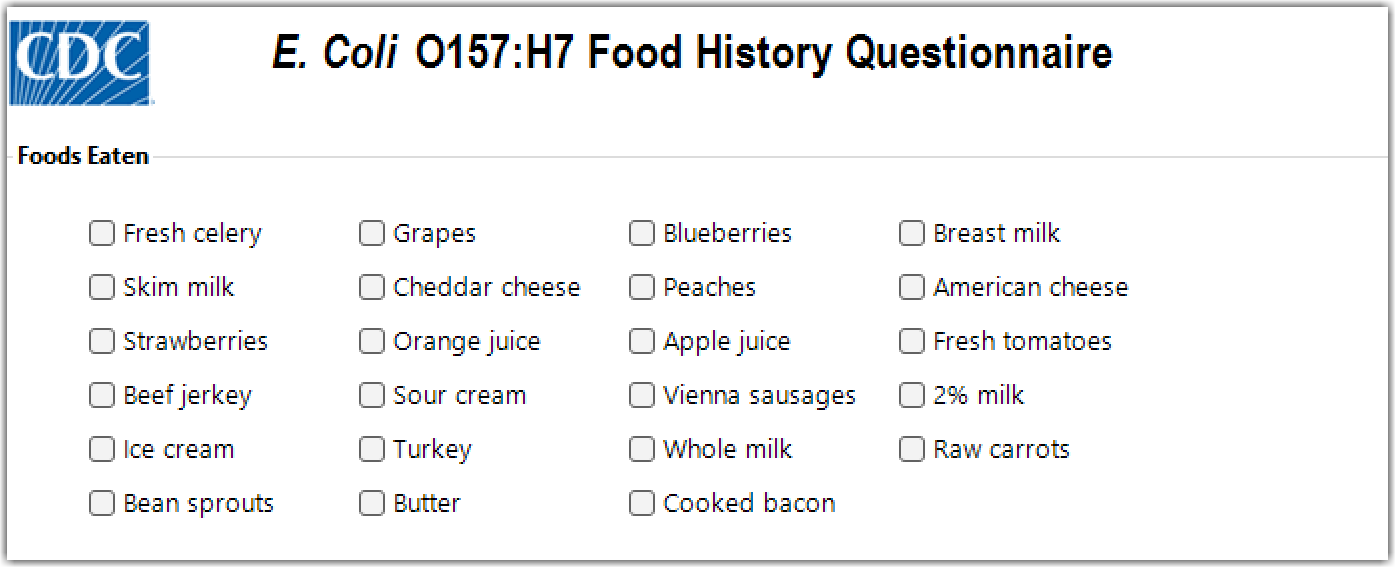
\includegraphics[width=\linewidth,height=0.4\textheight,keepaspectratio]{img/tableauDeBord/foodEaten}
	\caption{Liste des aliments consommés}
	\label{fig:foodeaten}
\end{figure}

Le gadget \kw{Table MxN / 2x2} sert à croiser deux variables qualitatives. Pour l'utiliser :
\begin{enumerate}
	\item Faire un clic droit sur le canevas, aller à \kw{Ajouter un gadget d'analyse} et choisir \kw{Table MxN / 2x2}. La fenêtre du gadget apparaît (\autoref{fig:tabulationcroise}) ;
	\item Dans le champ \kw{Exposition}, choisir la variable de l'exposition, ici \var{Icecream} ;
	\item Dans le champ \kw{Variable à de résultats} (libellé tel qu'il apparaît dans Epi Info), choisir la variable du résultat, ici \var{ILL}. Le champ \kw{Stratifier par} permet de stratifier l'analyse selon une troisième variable ;
	\item Valider par \kw{OK} (\autoref{fig:tabulationcroiseicecreamill}).
\end{enumerate}

\begin{figure}[H]
	\centering
	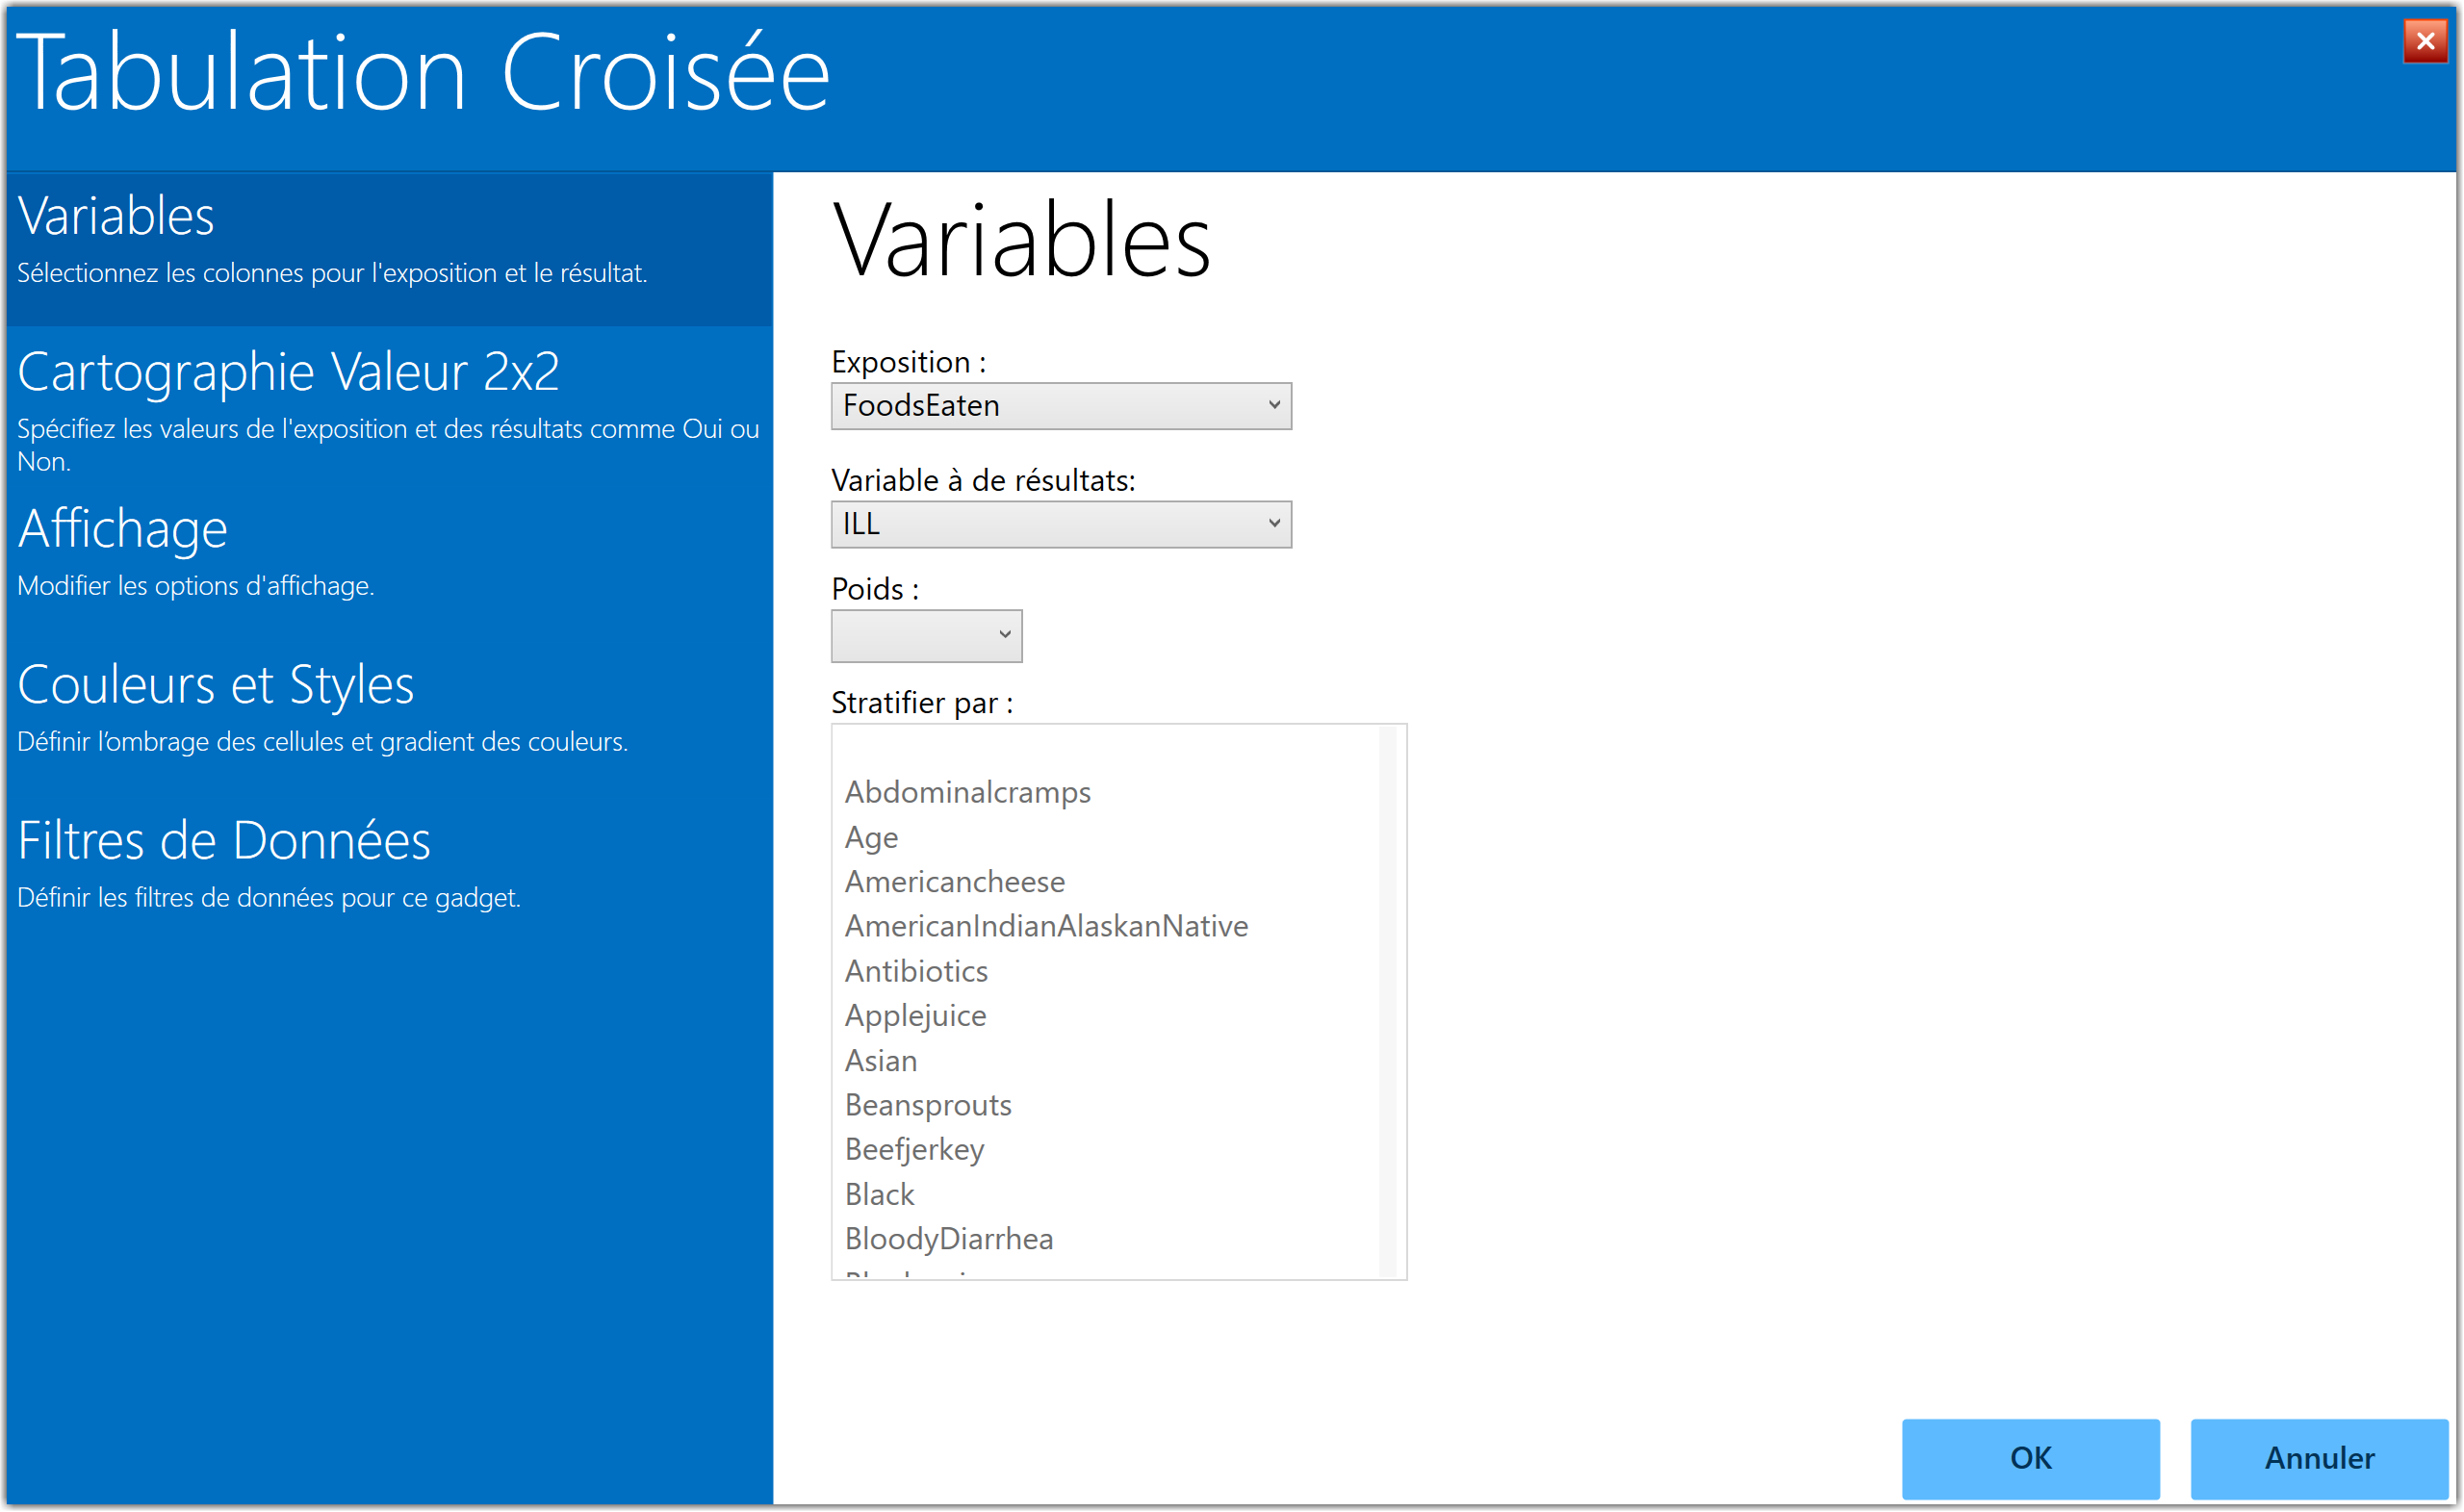
\includegraphics[width=\linewidth,height=0.4\textheight,keepaspectratio]{img/tableauDeBord/tabulationCroise}
	\caption{Fenêtre du gadget Table MxN / 2x2}
	\label{fig:tabulationcroise}
\end{figure}

\begin{figure}[H]
	\centering
	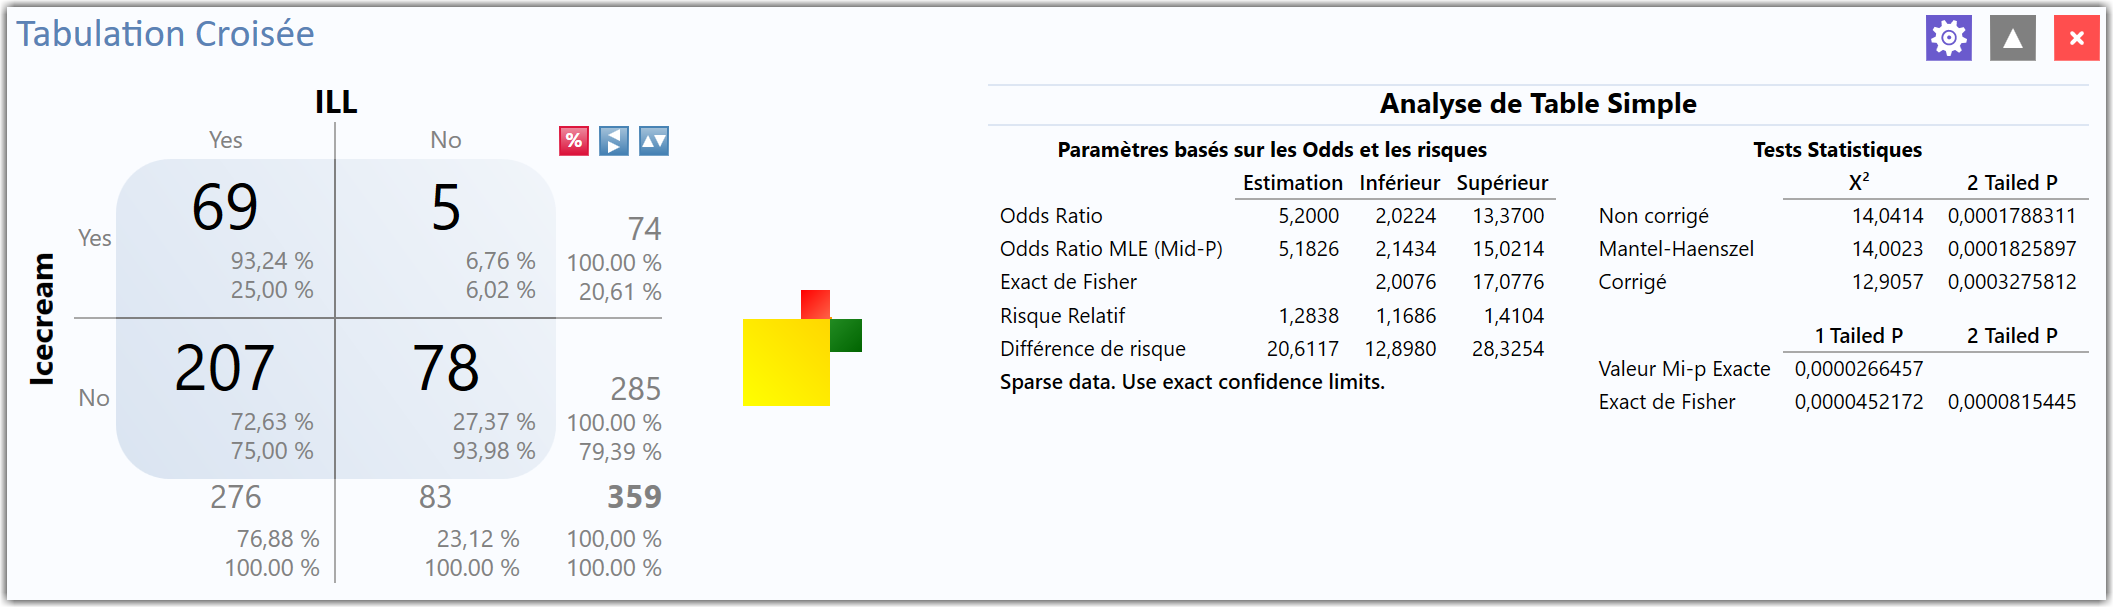
\includegraphics[width=\linewidth,height=0.4\textheight,keepaspectratio]{img/tableauDeBord/tabulationCroiseIcecreamIll}
	\caption{Association entre la consommation de crème glacée et la maladie}
	\label{fig:tabulationcroiseicecreamill}
\end{figure}

Pour que les mesures d'association aient leur sens épidémiologique habituel, la présence de l'exposition et la présence de la maladie doivent apparaître sur la première ligne et dans la première colonne du tableau. C'est le cas pour les variables Oui/Non d'Epi Info, qui sont triées automatiquement avec \kw{Yes} en premier. Les valeurs de la variable d'exposition s'affichent en lignes et celles de la variable de résultat en colonnes.

Pour un tableau 2x2, le gadget affiche :
\begin{itemize}
	\item le tableau croisé avec les effectifs et les pourcentages en ligne et en colonne ;
	\item l'\terme{odds ratio} et le \terme{risque relatif}, chacun avec son intervalle de confiance à 95~\% ;
	\item les tests statistiques : chi carré (non corrigé, de Mantel-Haenszel et corrigé de Yates) et, pour les petits effectifs, le test exact de Fisher, avec leurs valeurs \textit{p}.
\end{itemize}

Pour un tableau de plus de deux lignes ou deux colonnes (MxN), seul le chi carré est calculé.

L'interprétation se fait en deux temps. On lit d'abord la mesure d'association : un OR ou un RR supérieur à 1 suggère que la crème glacée est un facteur de risque. On vérifie ensuite si l'association est statistiquement significative : c'est le cas si la valeur \textit{p} est inférieure à 0,05, ou, ce qui revient au même, si l'intervalle de confiance à 95~\% ne contient pas la valeur 1.

Appliquons cette lecture à nos résultats (\autoref{fig:tabulationcroiseicecreamill}). Parmi les 74 personnes qui ont mangé de la crème glacée, 69 sont tombées malades, soit 93,24~\% ; parmi les 285 qui n'en ont pas mangé, 207 sont tombées malades, soit 72,63~\%. Le risque relatif vaut $0{,}9324/0{,}7263 = 1{,}28$ (IC à 95~\% : 1,17 à 1,41) : les consommateurs de crème glacée ont eu un risque de maladie 1,28 fois plus élevé que les autres. L'odds ratio vaut $(69 \times 78)/(5 \times 207) = 5{,}20$ (IC à 95~\% : 2,02 à 13,37). Le chi carré non corrigé vaut 14,04, avec une valeur \textit{p} de 0,0002. Les deux intervalles de confiance excluent 1 et la valeur \textit{p} est très inférieure à 0,05 : l'association entre la consommation de crème glacée et la maladie est statistiquement significative.

Remarquez l'écart entre l'OR (5,20) et le RR (1,28) : la maladie étant ici très fréquente (76,88~\% de malades), l'odds ratio surestime fortement le risque relatif. Dans une enquête de cohorte comme celle-ci, c'est le risque relatif qu'il faut privilégier.

\begin{mybox}[colbacktitle=CAUTION]{\faFire{} AVERTISSEMENT}
Une association statistiquement significative ne prouve pas un lien de causalité. Elle peut être due à un biais ou à un facteur de confusion. La conclusion doit toujours tenir compte du type d'enquête et des autres éléments disponibles.
\end{mybox}

\begin{mybox}[colbacktitle=TIP]{\faLightbulb{} CONSEIL}
Pour obtenir en une seule fois l'association entre la maladie et chacun des aliments répertoriés dans la base, sélectionnez dans le champ \kw{Exposition} la variable \var{FoodsEaten} au lieu de \var{Icecream}. \var{FoodsEaten} est le nom du groupe qui rassemble les aliments consommés (question \kw{Foods Eaten}) : le gadget calcule alors un tableau 2x2 pour chaque aliment.
\end{mybox}

\section{Recodage de variables}
\label{recodage}

Si l'on représente graphiquement la variable âge telle quelle, chaque valeur d'âge présente dans la base apparaît séparément, ce qui rend le graphique illisible. Il faut alors recoder l'âge en tranches d'âge.

Pour cela :
\begin{itemize}
	\item Survoler avec la souris le bord gauche du canevas, où se trouve un petit rectangle portant la mention \kw{Variables définies}. Le volet se déplie ; on peut lire en bas, de gauche à droite, \kw{Nouvelle variable}, \kw{Éditer variable} et \kw{Supprimer variable} ;
	\item Cliquer sur le premier bouton. Un sous-menu apparaît : cliquer sur \kw{Avec valeur transcodée} (\autoref{fig:recodervariable}) ;
	\item Une fenêtre d'édition s'ouvre :
	\begin{dingautolist}{192}
		\item Dans \kw{Champ de source}, sélectionner la variable \var{Age} ;
		\item Dans \kw{Champ de destination}, indiquer le nom de la nouvelle variable. Epi Info propose par défaut le nom de la variable d'origine suivi d'un tiret bas et du mot \var{RECODED}, ici \var{Age\_RECODED}. Vous pouvez le modifier ;
		\item Dans le champ \kw{Type du champ de destination}, choisir entre \kw{Text}, \kw{Numeric} et \kw{Yes/No}. Nous gardons le type \kw{Text}, car nous ne ferons pas de calculs sur la nouvelle variable ;
		\item Laisser cochée la case \kw{Maintient l'ordre de classement le cas échéant} ;
		\item Cliquer en bas de la fenêtre sur \kw{Saisir les valeurs de l'intervalle}. Rappelons que l'âge varie de 7 à 91 ans. Par défaut, Epi Info encadre les intervalles par les valeurs extrêmes (\commande{LOVALUE} pour le minimum et \commande{HIVALUE} pour le maximum). Dans la fenêtre \kw{Saisir les valeurs de l'intervalle}, nous saisissons la \kw{Valeur de début}, ici 5, la \kw{Valeur de fin}, ici 85, et dans la case \kw{Par} l'amplitude des tranches, ici 10 ans ;
		\item Valider par \kw{OK}, puis de nouveau par \kw{OK} (\autoref{fig:variableagerecoded} et \autoref{fig:resultatrecodageage}). Sur la \autoref{fig:resultatrecodageage}, remarquez les valeurs \commande{LOVALUE} et \commande{HIVALUE}, qui représentent les valeurs extrêmes. De retour sur le canevas, la nouvelle variable figure dans le volet \kw{Variables définies}, où l'on peut la modifier.
	\end{dingautolist}
\end{itemize}

\begin{mybox}[colbacktitle=CAUTION]{\faFire{} AVERTISSEMENT}
Si vous quittez le Tableau de bord sans l'avoir sauvegardé, vous perdrez les variables que vous avez créées. Nous verrons à la section~\ref{sauvegarderTableauDeBord}, \nameref{sauvegarderTableauDeBord}, page~\pageref{sauvegarderTableauDeBord}, comment sauvegarder l'espace de travail.
\end{mybox}

\begin{figure}[H]
	\centering
	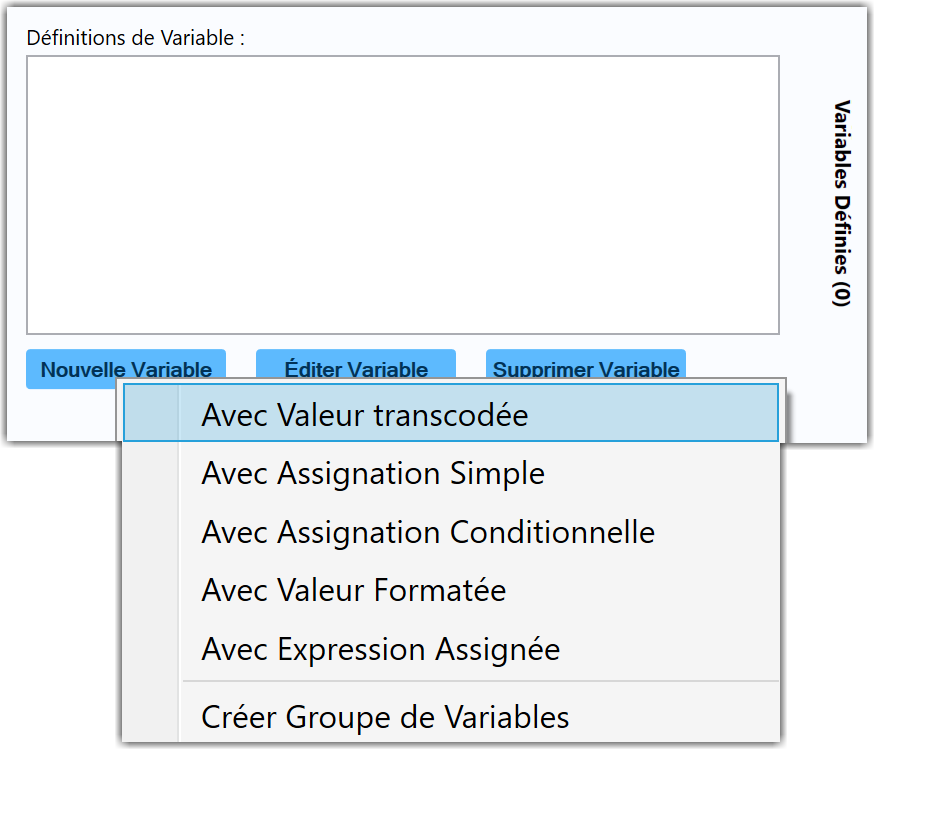
\includegraphics[width=\linewidth,height=0.4\textheight,keepaspectratio]{img/tableauDeBord/recoderVariable}
	\caption{Procédure de recodage de l'âge}
	\label{fig:recodervariable}
\end{figure}

\begin{figure}[H]
	\centering
	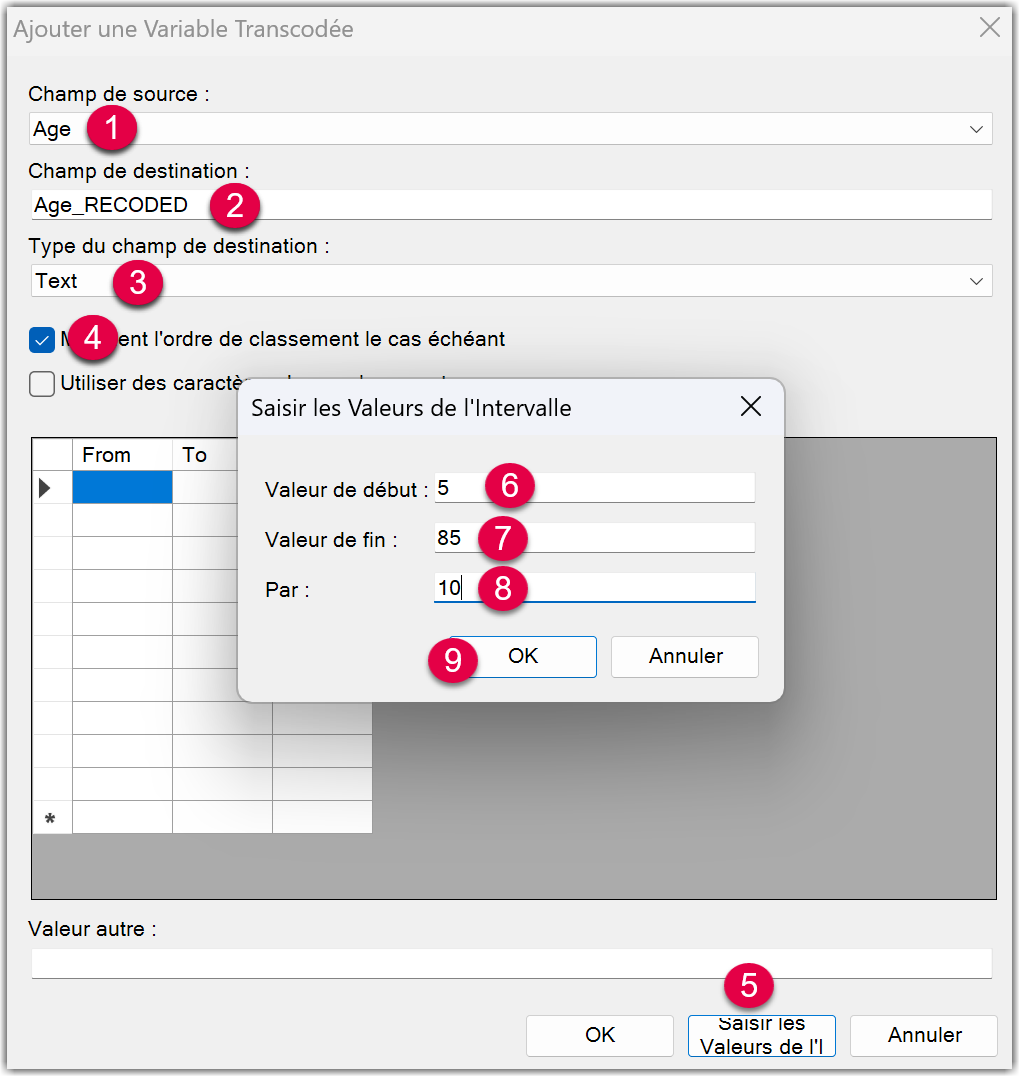
\includegraphics[width=\linewidth,height=0.4\textheight,keepaspectratio]{img/tableauDeBord/variableAgeRecoded}
	\caption{Recodage de la variable Age en tranches d'âge}
	\label{fig:variableagerecoded}
\end{figure}

\begin{figure}[H]
	\centering
	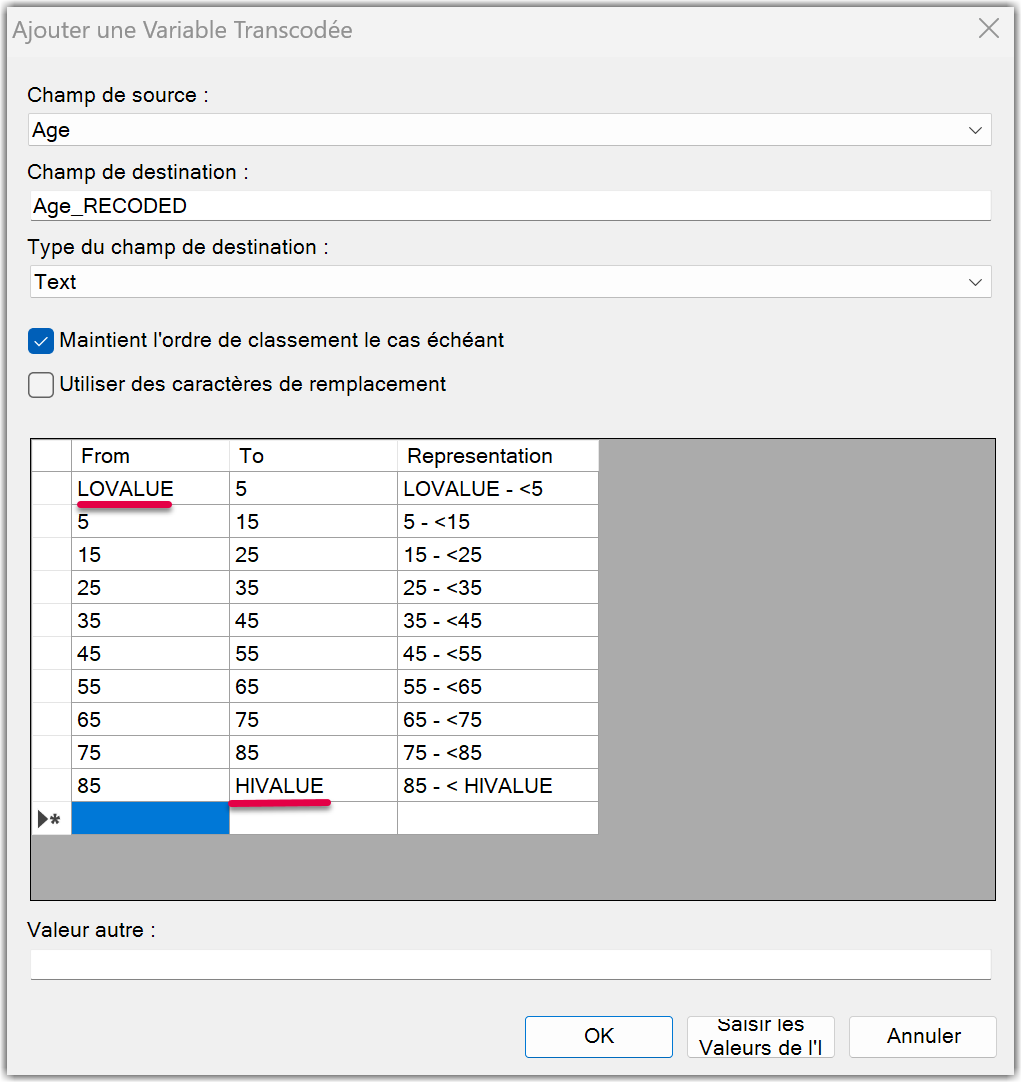
\includegraphics[width=\linewidth,height=0.4\textheight,keepaspectratio]{img/tableauDeBord/resultatRecodageAge}
	\caption{Résultat du recodage de la variable Age en tranches d'âge}
	\label{fig:resultatrecodageage}
\end{figure}

\section{Utiliser des filtres de données}

Les filtres permettent de restreindre l'analyse à une partie des données. Cherchons par exemple le nombre d'\kw{hommes malades âgés de 25 à 35 ans} :

\begin{itemize}
	\item Survoler avec la souris la petite zone rectangulaire située sur le bord droit du canevas. Le volet \kw{Filtres de données} se déplie :
	\begin{dingautolist}{192}
		\item Dans la partie \kw{Nom de champ}, sélectionner la variable \var{ILL} ;
		\item Dans la partie \kw{Opérateur}, choisir l'opérateur souhaité, ici \kw{est égal à} ;
		\item Choisir enfin la valeur, ici \kw{Yes}. Très facile, n'est-ce pas ? \emoji{smiling-face-with-smiling-eyes}
		\item Cliquer sur \kw{Ajouter un filtre}. Le filtre \question{La valeur de [ILL] est égal à Yes} apparaît dans la case \kw{Filter criteria} de la partie \kw{Filtres de données}. Pour ajouter un deuxième filtre, on recommence la procédure ;
		\item Sélectionner cette fois la variable \var{Sex} ;
		\item Choisir \kw{est égal à} dans la partie \kw{Opérateur} ;
		\item Dans la partie valeur, toutes les modalités de la variable \var{Sex} s'affichent ; sélectionner \kw{M-Male} ;
		\item Cliquer sur \kw{Ajouter un filtre} puis, dans le menu qui apparaît, sur \kw{Ajouter avec ET} (on pourrait aussi choisir \kw{Ajouter avec OU}). Le deuxième filtre, \question{La valeur de [Sex] est égal à M-Male}, s'ajoute avec l'opérateur logique \kw{and} ;
		\item Ajouter le dernier filtre de la même manière, mais en choisissant la variable \var{Age} et l'opérateur \kw{entre} ;
		\item Saisir les bornes de l'âge, 25 et 35, puis cliquer sur \kw{Ajouter avec ET}. Le troisième filtre, \question{La valeur de Age est comprise entre 25 et 35}, s'ajoute avec l'opérateur logique \kw{and} dans la colonne \kw{Join} (\autoref{fig:filtre}, \autoref{fig:filtreajouteret} et \autoref{fig:filtreresultat}).
	\end{dingautolist}
\end{itemize}

Le filtre fonctionne : 39 enregistrements sont désormais visibles en haut à droite. Les filtres permettent de travailler sur une partie des données définie à l'avance. Attention : un filtre s'applique à tous les gadgets du canevas, y compris ceux créés avant lui, dont les résultats sont recalculés.
Une note apparaît aussi sur le canevas : \question{Les filtres de toile suivants sont en vigueur : la valeur de [ILL] est égal à Yes and La valeur de [Sex] est égal à M-Male and La valeur de Age est comprise entre 25 et 35}.

\begin{mybox}[colbacktitle=CAUTION]{\faFire{} AVERTISSEMENT}
Lorsque vous appliquez des filtres, vérifiez toujours sur quelle partie des données vous travaillez, en contrôlant régulièrement le nombre d'enregistrements affiché.
\end{mybox}

\begin{figure}[H]
	\centering
	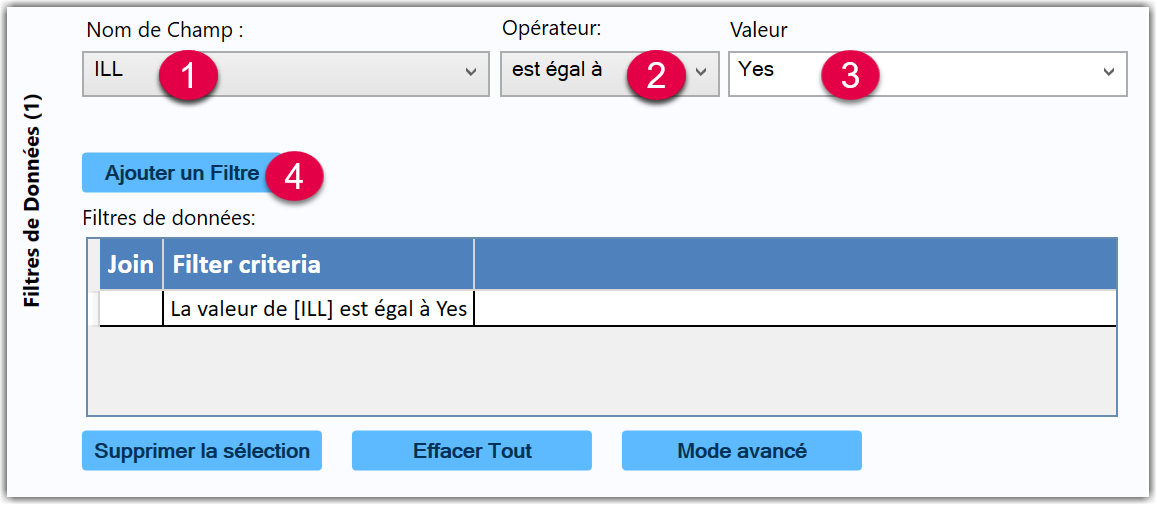
\includegraphics[width=\linewidth,height=0.4\textheight,keepaspectratio]{img/tableauDeBord/filtre}
	\caption{Ajouter un filtre de données}
	\label{fig:filtre}
\end{figure}

\begin{figure}[H]
	\centering
	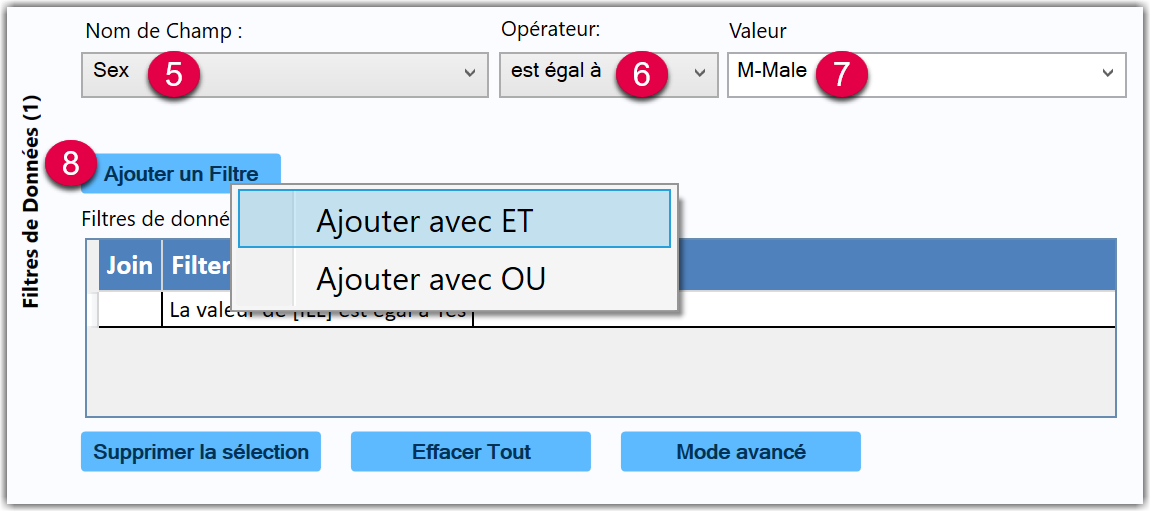
\includegraphics[width=\linewidth,height=0.4\textheight,keepaspectratio]{img/tableauDeBord/filtreAjouterEt}
	\caption{Ajouter un deuxième filtre avec un opérateur logique}
	\label{fig:filtreajouteret}
\end{figure}

\begin{figure}[H]
	\centering
	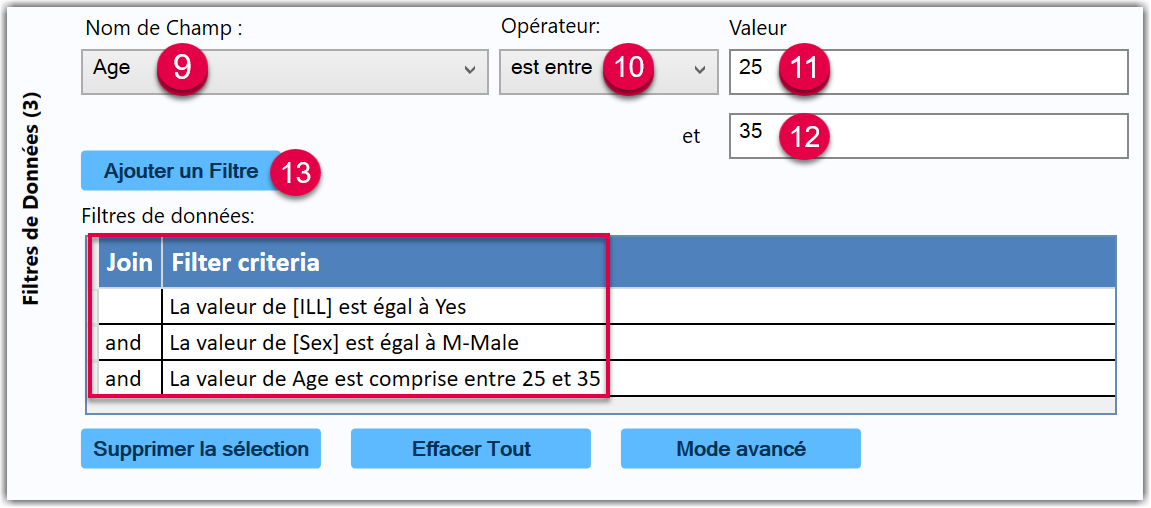
\includegraphics[width=\linewidth,height=0.4\textheight,keepaspectratio]{img/tableauDeBord/filtreResultat}
	\caption{Résultat du filtre : femmes malades âgées de 25 à 35 ans}
	\label{fig:filtreresultat}
\end{figure}

\section{Représentations graphiques}
Il est possible, et très facile, de réaliser des graphiques dans Epi Info 7 : diagrammes en barres, histogrammes, diagrammes en secteurs (camemberts), etc.
De façon générale, on procède comme suit :

\begin{enumerate}
	\item Faire un clic droit sur le canevas ;
	\item Sélectionner \kw{Ajouter un gadget d'analyse} ;
	\item Sélectionner \kw{Graphiques} ;
	\item Choisir le type de graphique : \kw{Colonne} pour un diagramme en barres, \kw{Secteur} pour un camembert, etc. ;
	\item La fenêtre de paramétrage du graphique s'ouvre.
\end{enumerate}

\subsection{Exemple : la distribution des tranches d'âge}
Représentons graphiquement la variable \var{Age\_RECODED} créée à la section~\ref{recodage}. Les tranches d'âge étant des classes d'une variable quantitative, nous utilisons un graphique en colonnes jointives, à la manière d'un histogramme. Nous procédons comme indiqué ci-dessus en sélectionnant \kw{Graphique de la colonne} (\autoref{fig:representationhistogramme}). Une fenêtre s'ouvre pour paramétrer le graphique (\autoref{fig:customisationhistogramme}). Voici comment obtenir le graphique de la \autoref{fig:resultathistogramme} :

\begin{description}
	\item[A] \kw{Variables} : choisir la variable à représenter dans \kw{Variable principale}, ici \var{Age\_RECODED}. On peut aussi demander un graphique pour chaque valeur d'une autre variable ;
	\item[B] \kw{Regroupement et Tri} : définir l'ordre de tri des barres et créer des groupes ;
	\item[C] \kw{Affichage} : modifier les options d'affichage, comme les dimensions du graphique ;
	\item[D] \kw{Couleurs et Styles} : modifier les couleurs, l'ombrage et l'espace entre les barres (le réduire à zéro pour des colonnes jointives) ;
	\item[E] \kw{Étiquettes} : donner un titre au graphique, nommer les axes, etc. ;
	\item[F] \kw{Légende} : régler les options de la légende ;
	\item[G] \kw{Filtres de données} : appliquer un filtre propre à ce graphique.
\end{description}

\begin{figure}[H]
	\centering
	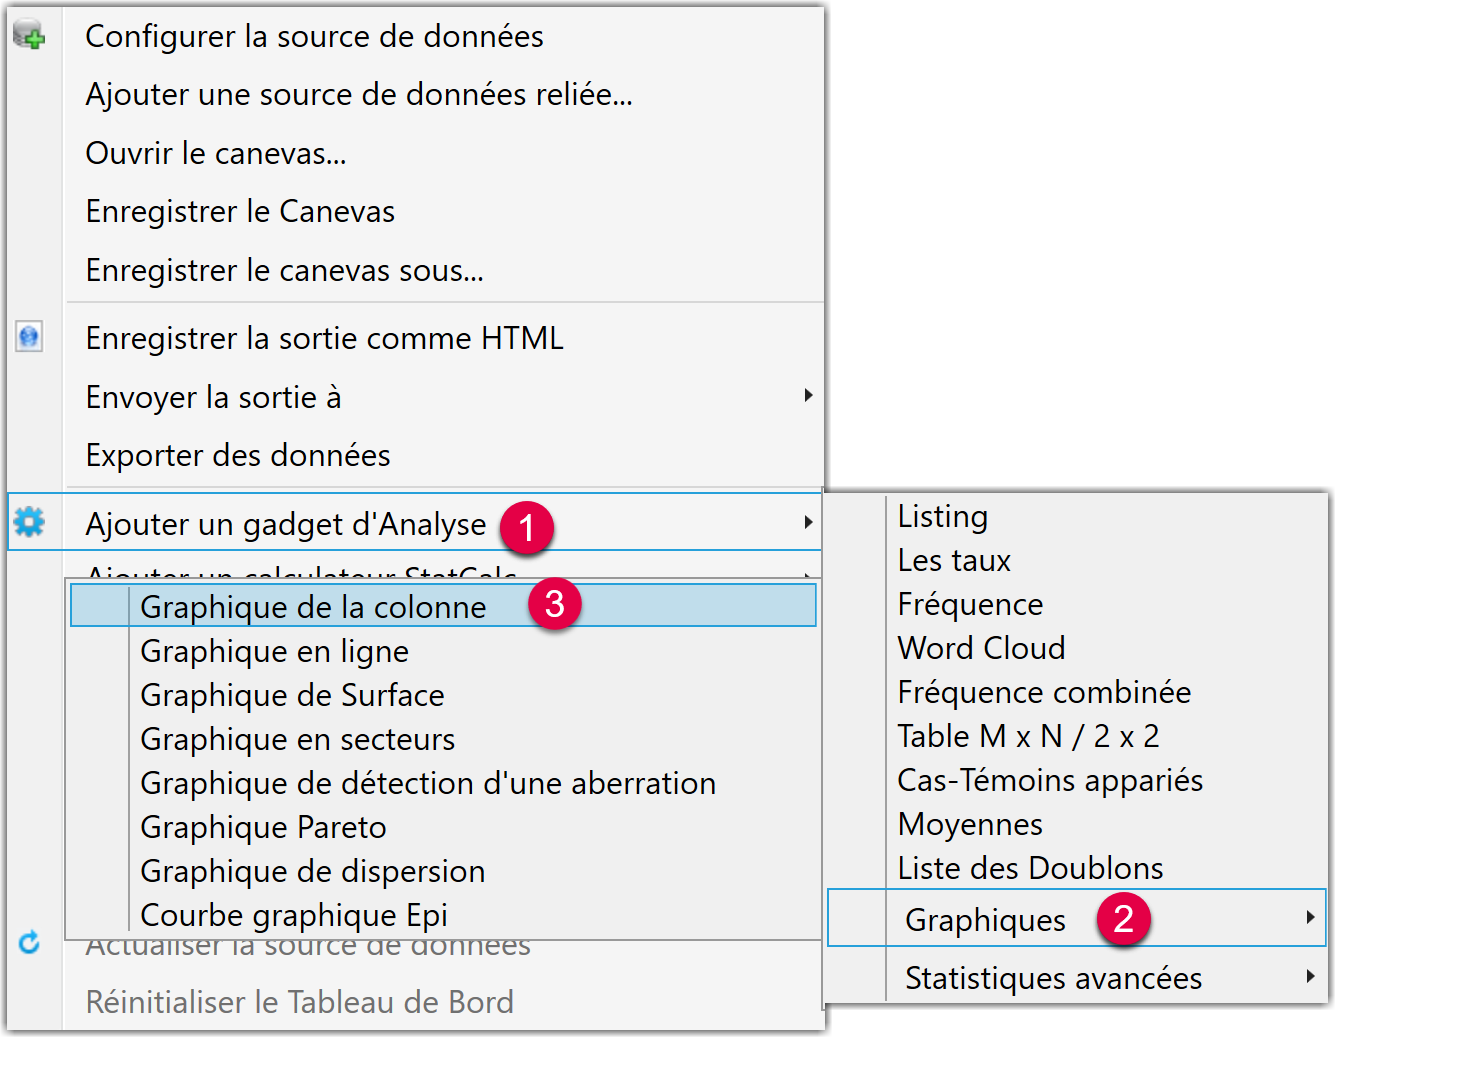
\includegraphics[width=\linewidth,height=0.4\textheight,keepaspectratio]{img/tableauDeBord/representationHistogramme}
	\caption{Procédure de représentation graphique des tranches d'âge}
	\label{fig:representationhistogramme}
\end{figure}

\begin{figure}[H]
	\centering
	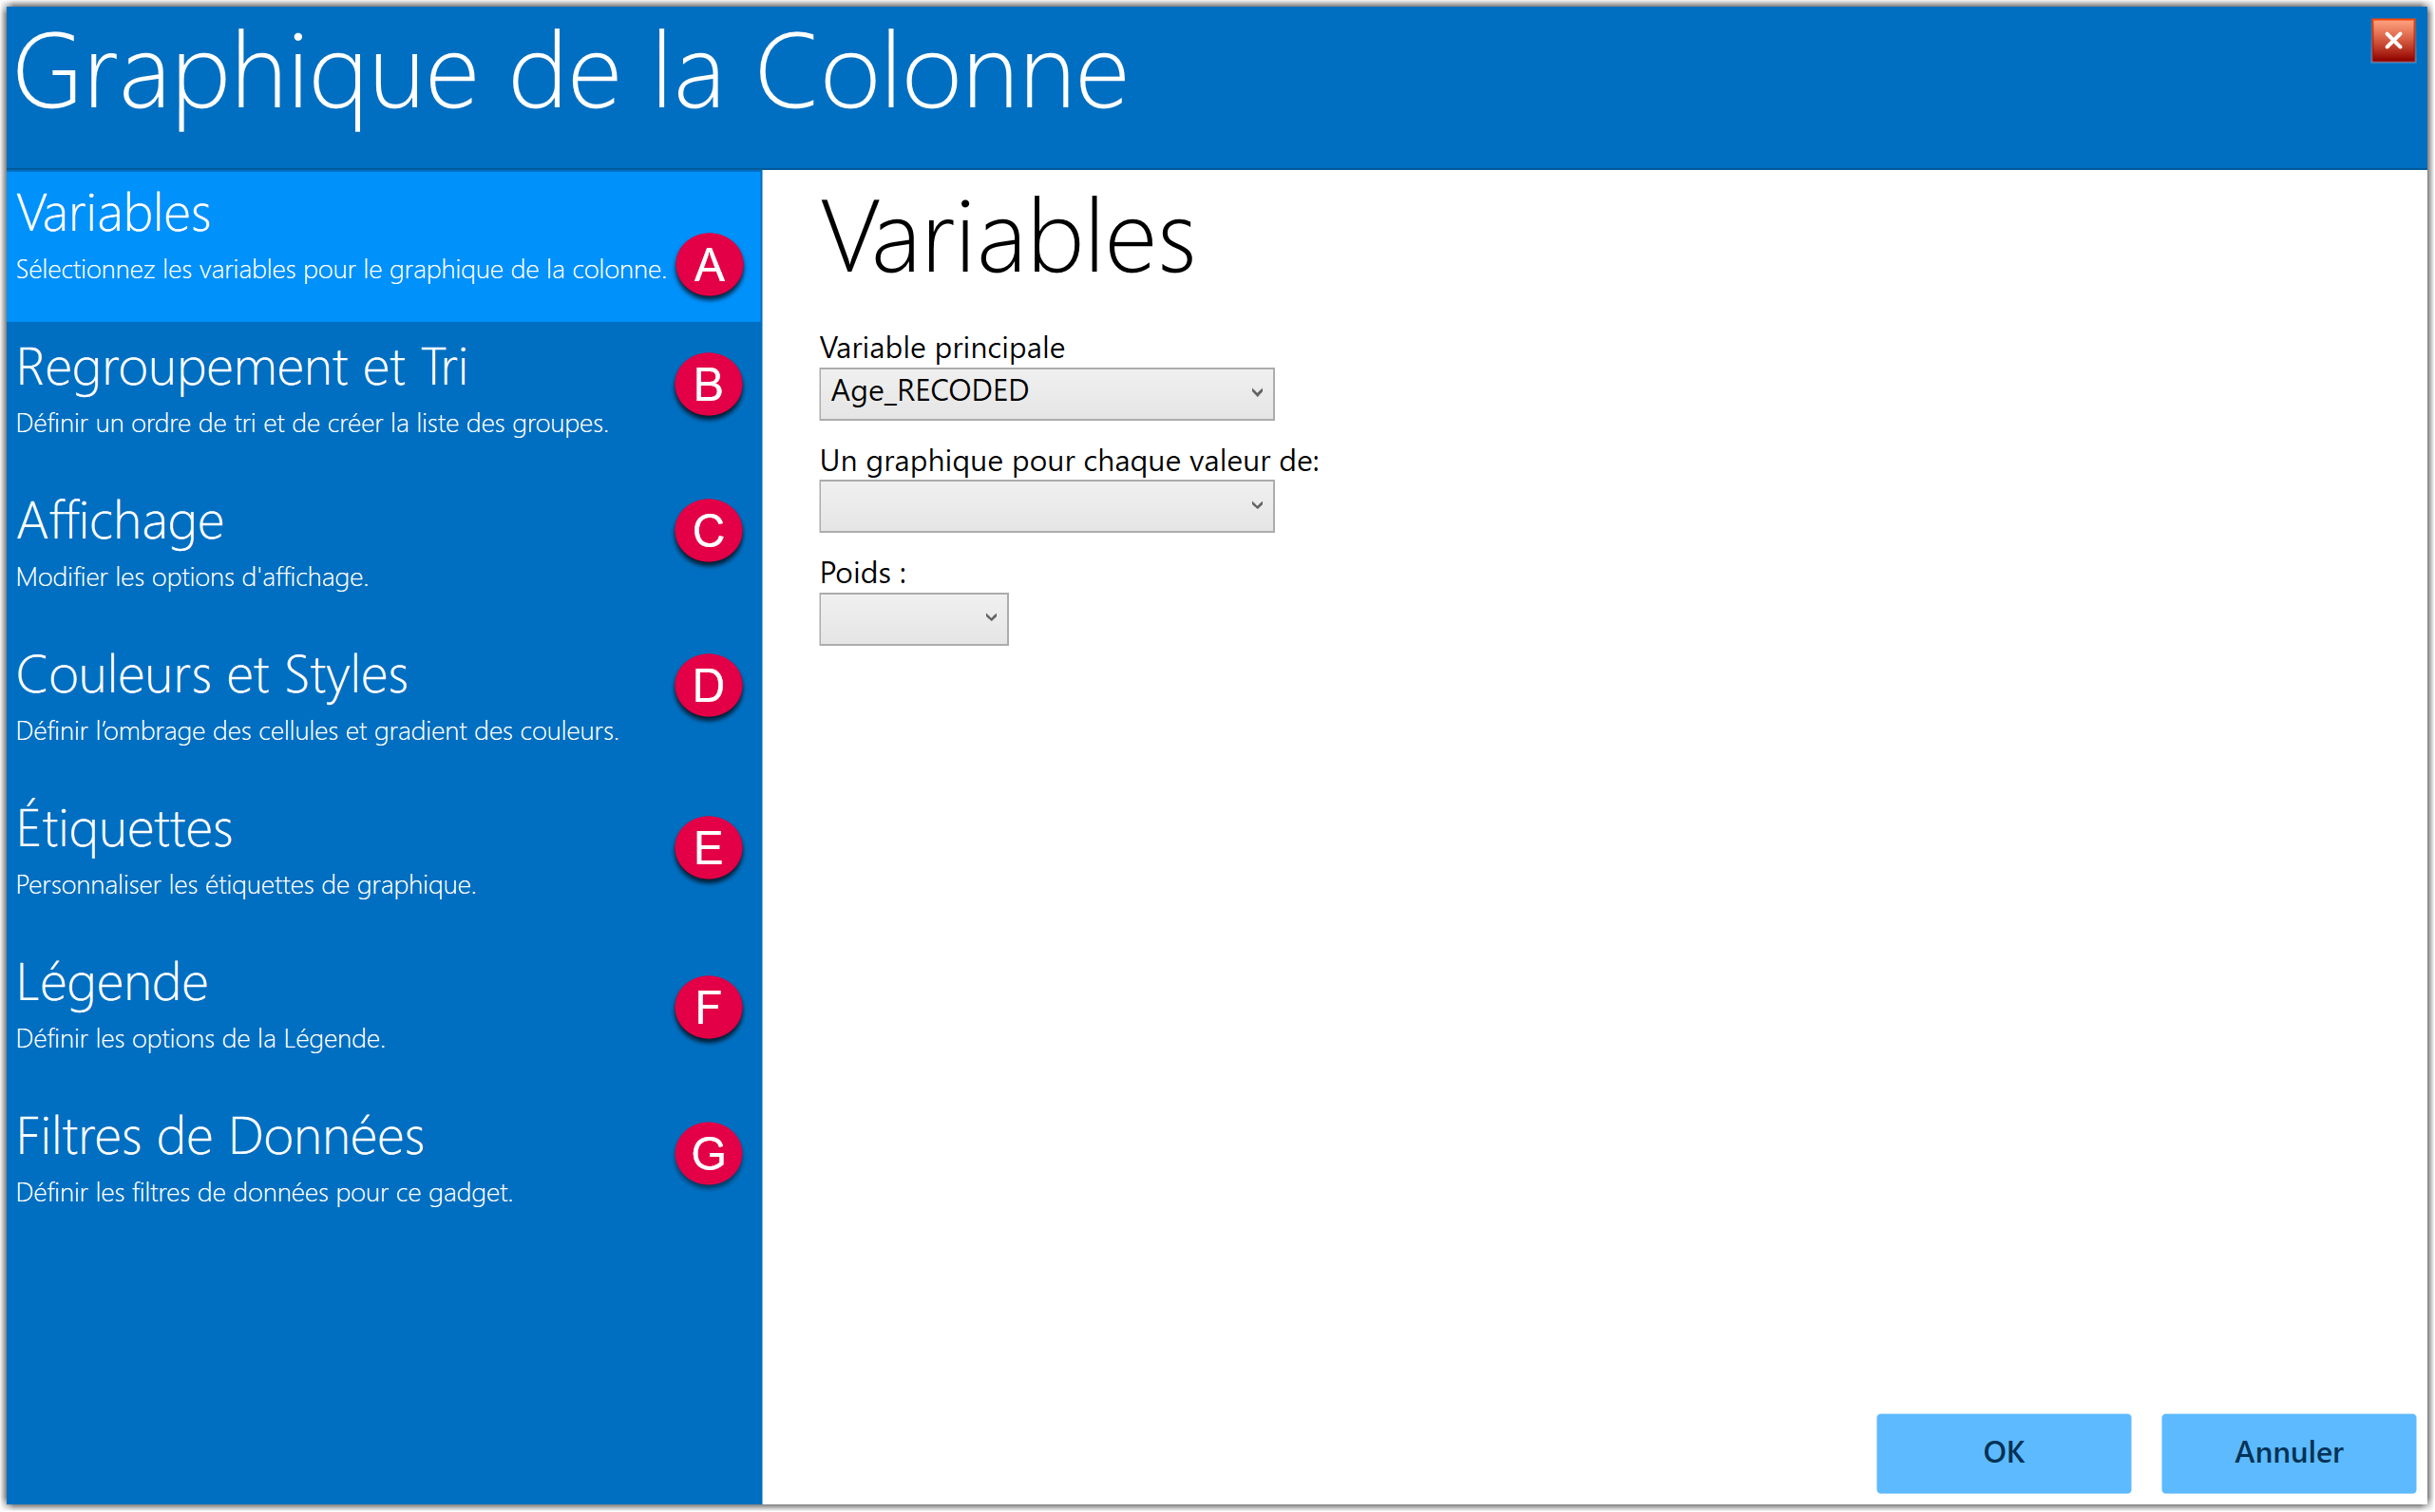
\includegraphics[width=\linewidth,height=0.4\textheight,keepaspectratio]{img/tableauDeBord/customisationHistogramme}
	\caption{Paramétrage du graphique}
	\label{fig:customisationhistogramme}
\end{figure}

\begin{figure}[H]
	\centering
	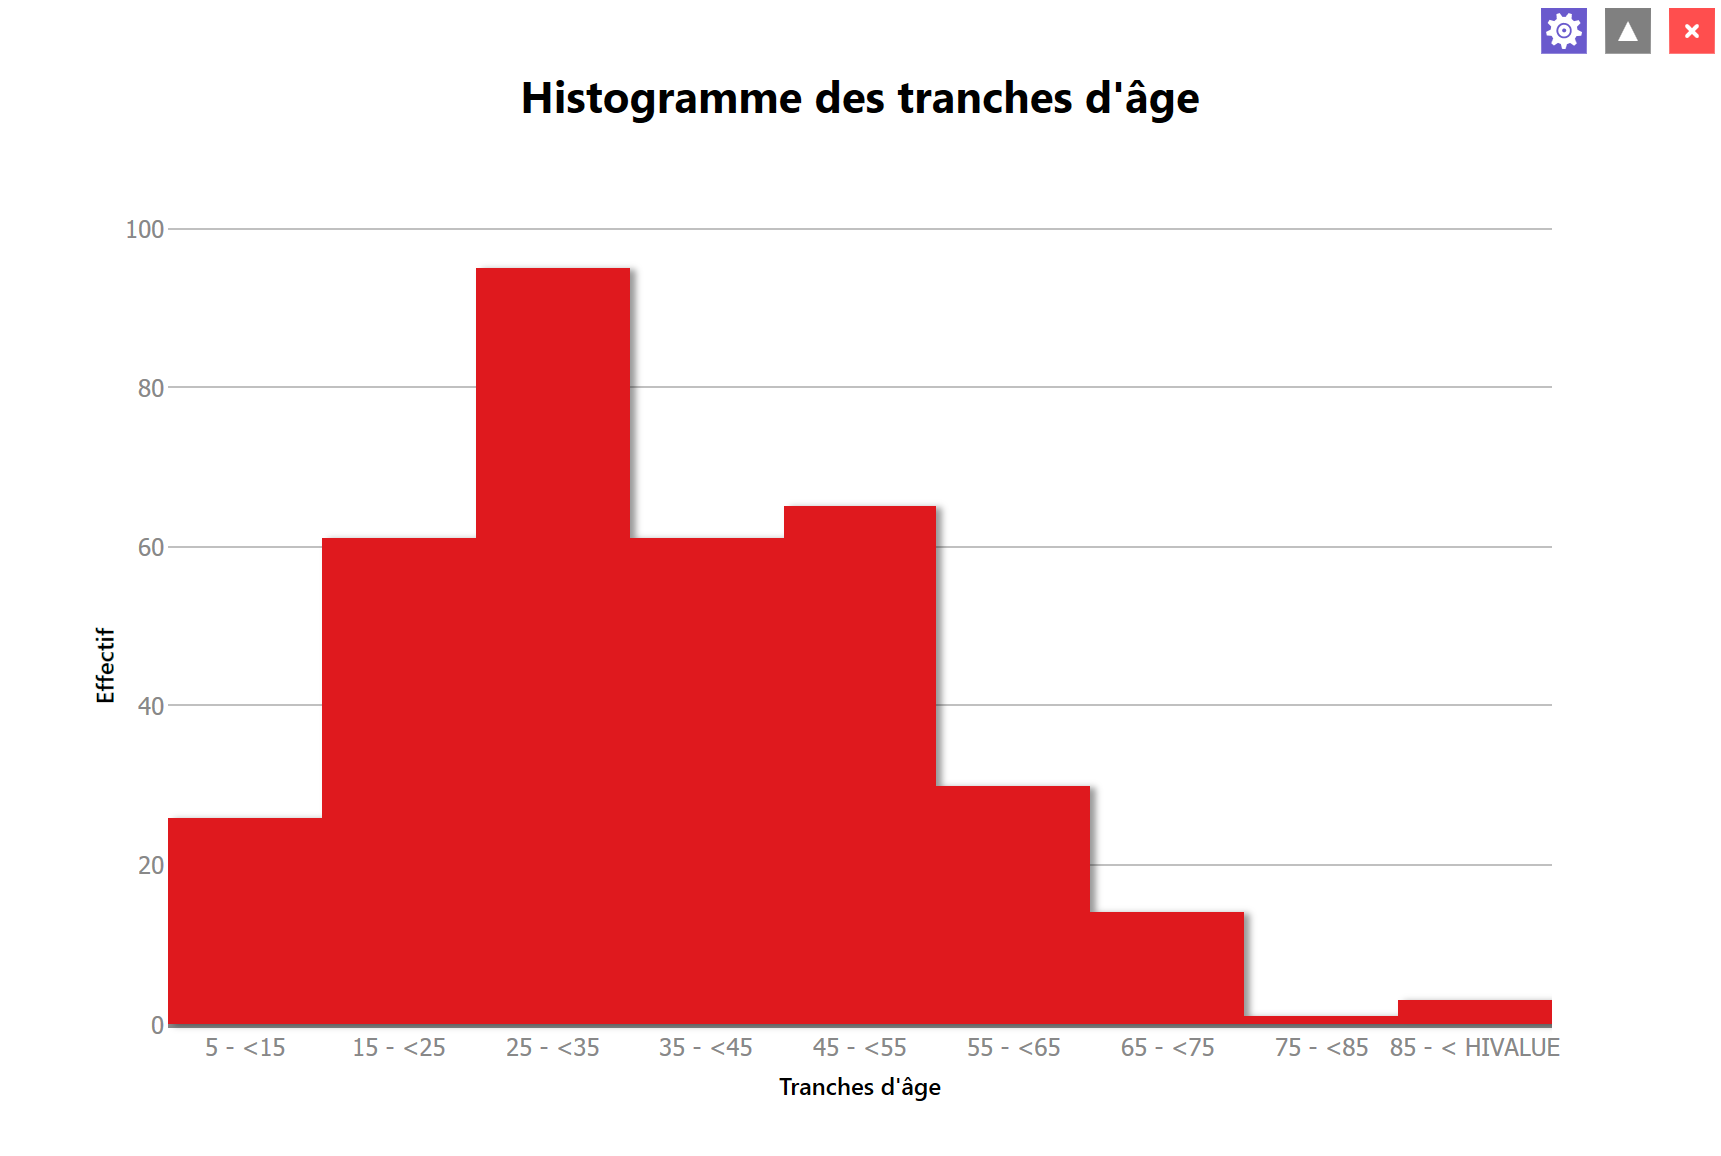
\includegraphics[width=\linewidth,height=0.4\textheight,keepaspectratio]{img/tableauDeBord/resultatHistogramme}
	\caption{Distribution des tranches d'âge}
	\label{fig:resultathistogramme}
\end{figure}

Le graphique peut être enregistré sous forme d'image au format PNG\footnote{\emph{Portable Network Graphics}.} (.png) ou JPEG\footnote{\emph{Joint Photographic Experts Group}.} (.jpg).

\begin{mybox}[colbacktitle=IMPORTANT]{\faExclamationCircle{} IMPORTANT}
Cette section montre qu'il est tout à fait possible de réaliser des graphiques dans Epi Info. En pratique, nous préférerons souvent exporter nos résultats vers un logiciel comme Microsoft Excel ou LibreOffice Calc, pour profiter de leurs nombreuses possibilités graphiques.
\end{mybox}

\section{Exporter des données au format Excel ou CSV}

Il est possible d'exporter les données d'Epi Info au format tableur Excel ou au format CSV\footnote{\emph{Comma-Separated Values} : format de fichier texte ouvert dans lequel les valeurs sont séparées par des virgules.}.
Pour cela, faire un clic droit sur le canevas et choisir \kw{Exporter des données}. Une fenêtre s'ouvre. De haut en bas :
\begin{itemize}
	\item dans la partie \kw{Output Mode}, laisser cochée l'option \kw{Append} ;
	\item dans \kw{Format de sortie}, choisir le format Excel, ici \kw{Microsoft Excel 97-2003 Workbook (.xls)} ;
	\item au niveau de \kw{Information de connexion}, cliquer sur \kw{Parcourir}. Une fenêtre s'ouvre : vérifier que la case \kw{First row contains header information} est bien cochée, choisir l'emplacement du fichier exporté et saisir son nom ;
	\item au niveau de la \kw{Table de destination}, saisir le nom de la table, ici \var{enquete} ;
	\item dans \kw{Champs à exporter}, sélectionner les champs à exporter, ou toute la base ;
	\item on peut laisser cochée la case \kw{Trier les variables par ordre de tabulation} ;
	\item cliquer enfin sur \kw{Exporter} (\autoref{fig:exportexcel}).
\end{itemize}

Lorsque l'export a réussi, un message s'affiche en bas de la fenêtre, ici \question{Exportation terminée avec succès. 359 enregistrements écrits.}

\begin{figure}[H]
	\centering
	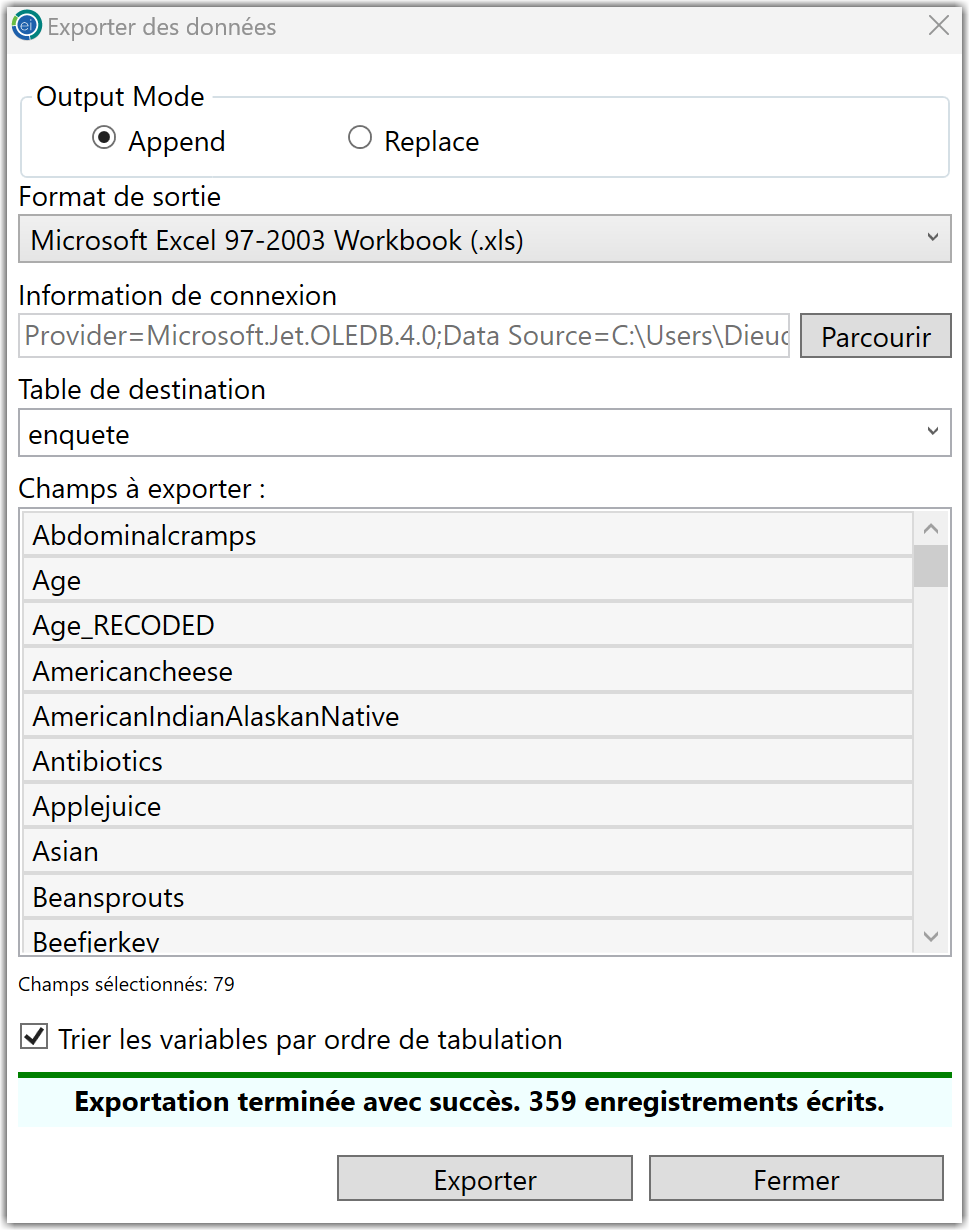
\includegraphics[width=\linewidth,height=0.4\textheight,keepaspectratio]{img/tableauDeBord/exportExcel}
	\caption{Exporter des données vers Excel}
	\label{fig:exportexcel}
\end{figure}

\begin{mybox}[colbacktitle=TIP]{\faLightbulb{} CONSEIL}
Pour exporter au format CSV, choisissez CSV dans \kw{Format de sortie}.
\end{mybox}

\begin{mybox}[colbacktitle=NOTE]{\faInfoCircle{} À RETENIR}
Le format \kw{.xls} (Excel 97-2003) s'ouvre sans difficulté dans toutes les versions d'Excel et dans LibreOffice Calc. Selon les versions d'Epi Info et les composants installés sur l'ordinateur, le format plus récent \kw{.xlsx} peut aussi être proposé ; sur les anciennes versions, il fallait installer un connecteur pour exporter aux formats Excel 2007 et Access 2007.
\end{mybox}

\section{Copier un résultat d'analyse vers Excel}

Comme nous l'avons vu, nous pouvons être amenés à transférer nos résultats vers un tableur, Microsoft Excel ou LibreOffice Calc par exemple, pour réaliser nos graphiques.
Pour cela, faire un clic droit sur le gadget d'analyse concerné, puis cliquer sur \kw{Copy data to clipboard} (que nous recommandons) ou sur \kw{Send data to Excel}. Avec la première option, vous pouvez coller plusieurs résultats sur une même feuille Excel ; la seconde ouvre à chaque fois un nouveau classeur Excel. Testez les deux : chacune vous sera utile selon les cas.

\section{Sauvegarder son espace de travail}
\label{sauvegarderTableauDeBord}

Dans le module \module{tableau de bord visuel}, les gadgets d'analyse sont disposés sur le canevas : vous pouvez les déplacer, les réduire, les agrandir et les modifier.

Avant de quitter le module, que vous ayez fini ou non vos analyses, il est essentiel de sauvegarder votre espace de travail.
Pour cela, cliquer sur l'icône en forme de disquette, en haut à gauche dans l'en-tête (\autoref{fig:interfacetableaubord}), ou faire un clic droit sur le canevas et choisir \kw{Enregistrer le Canevas}. Au survol de la souris, la mention \kw{Enregistrer le tableau de bord en cours} s'affiche. Cliquer dessus, donner un nom au fichier, dont l'extension sera \var{.cvs7}, puis cliquer sur \kw{Enregistrer}. Vous pouvez ensuite quitter le logiciel sans risque. Pour reprendre vos analyses, ouvrez le \module{tableau de bord visuel}, cliquez sur l'icône \kw{Ouvrir} de l'en-tête, en forme de dossier ouvert, puis cherchez votre fichier.

Epi Info 7 est également fourni avec des tableaux de bord d'exemple, réalisés à partir des bases de données livrées avec le logiciel. Les ouvrir est un bon moyen de découvrir d'autres gadgets.

\chapter{Module Classique}
\label{moduleClassic}
%\minitoc

Pour l'analyse des données, Epi Info 7 propose deux modules : \module{tableau de bord visuel}, étudié au chapitre précédent, et \module{classique}. Dans ce chapitre, nous apprendrons à réaliser des analyses statistiques avec le module \module{classique}, qui fonctionne à l'aide de commandes.

\section{Découvrir le module Classique}

Pour ouvrir le module, cliquer sur \module{classique} dans la fenêtre d'accueil d'Epi Info (\autoref{fig:ouvrirmoduleclassique}).

\begin{figure}[H]
	\centering
	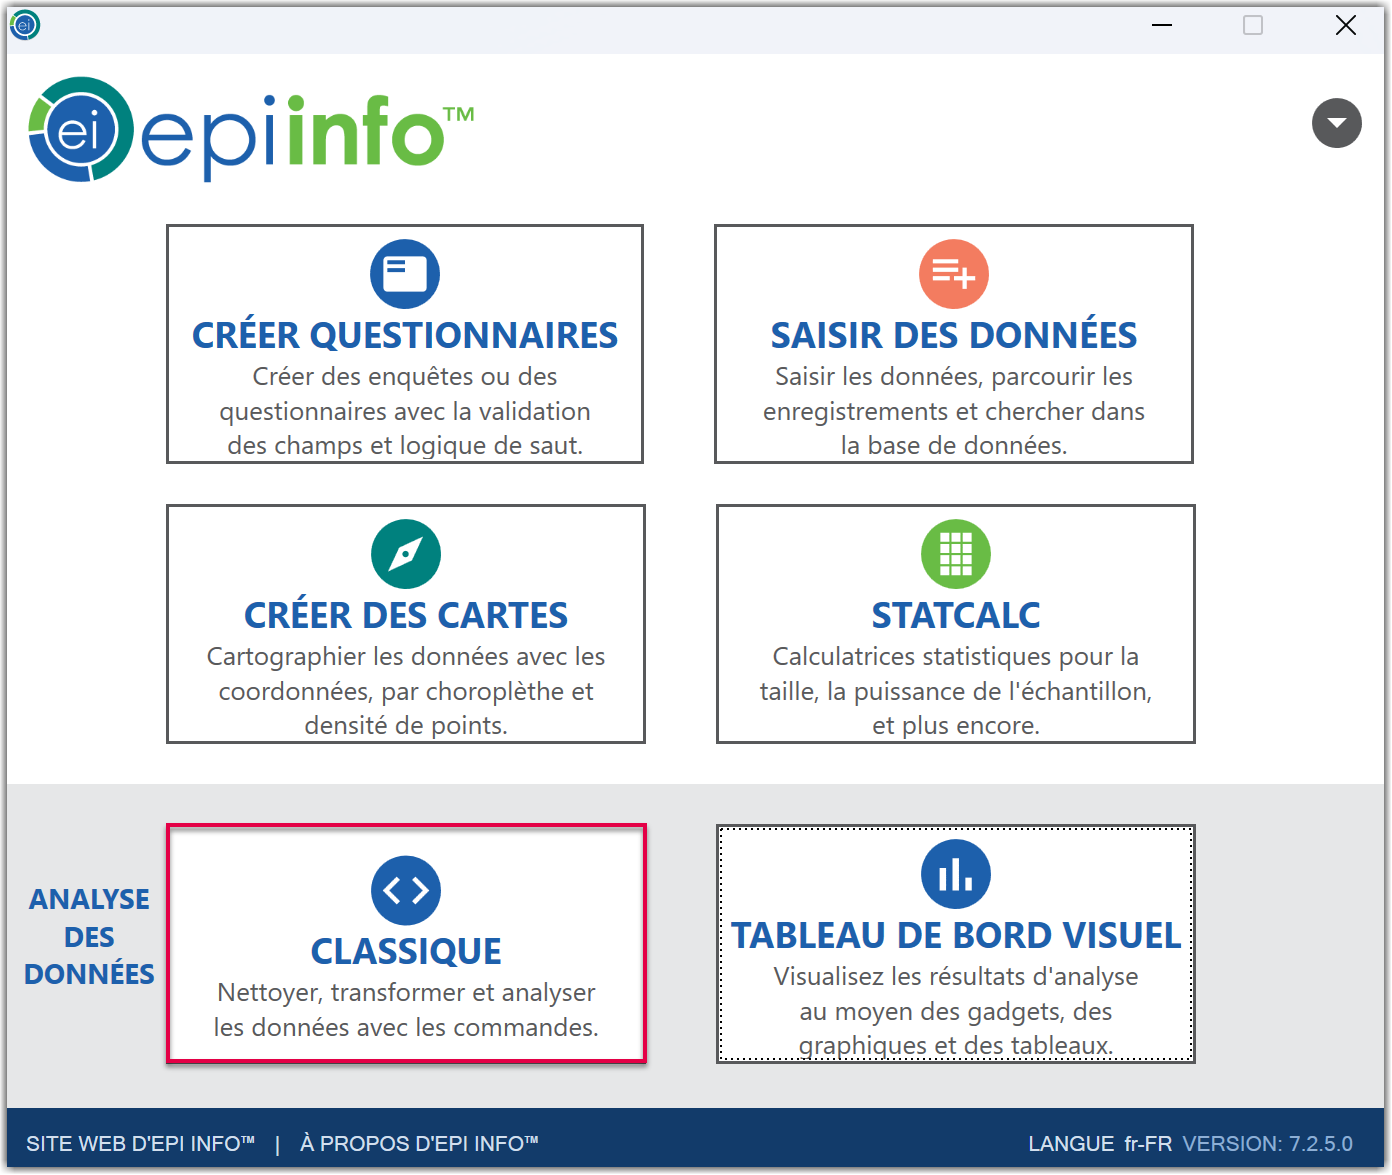
\includegraphics[width=\linewidth,height=0.4\textheight,keepaspectratio]{img/Classique/ouvrirModuleClassique}
	\caption{Ouvrir le module Classique}
	\label{fig:ouvrirmoduleclassique}
\end{figure}

L'interface du module comporte quatre parties (\autoref{fig:interfaceclassic}) : à gauche, la liste des commandes, regroupées par sections ; l'éditeur de programme, où s'écrivent les commandes ; la fenêtre des résultats ; et, tout en bas, la zone d'affichage des messages d'erreur.

\begin{figure}[H]
	\centering
	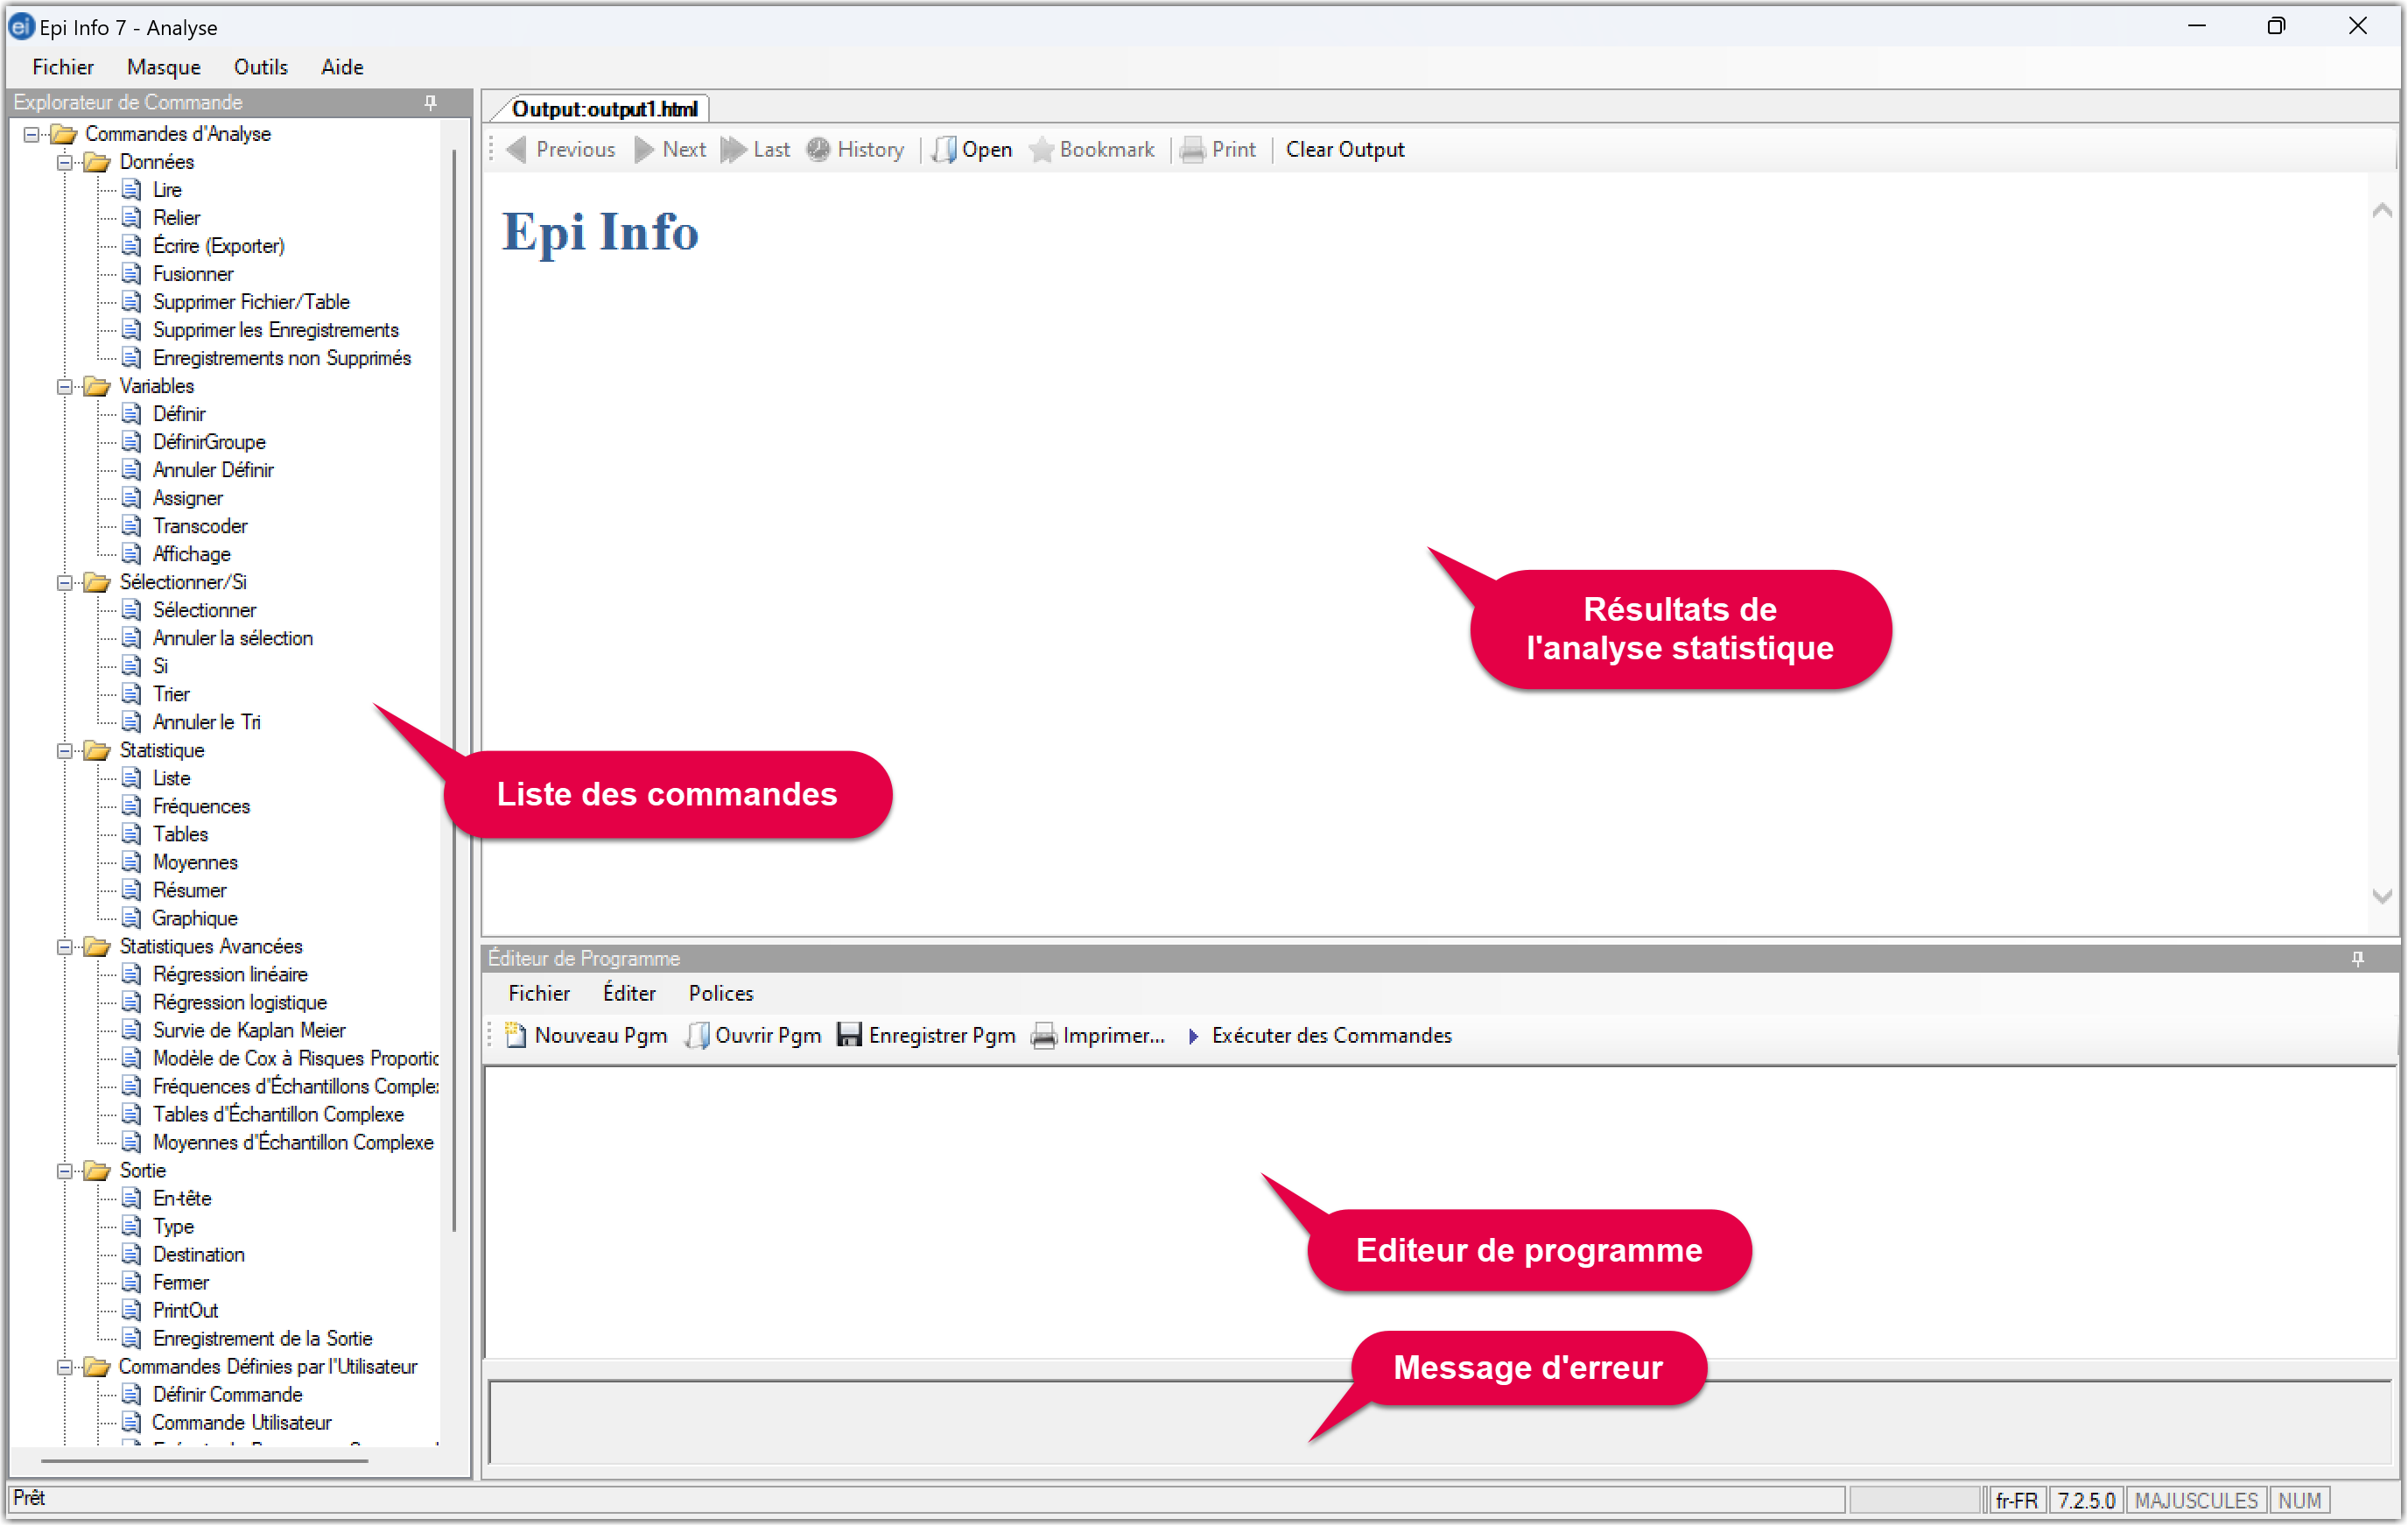
\includegraphics[width=\linewidth,height=0.4\textheight,keepaspectratio]{img/Classique/interfaceClassic}
	\caption{Interface du module d'analyse Classique}
	\label{fig:interfaceclassic}
\end{figure}

L'analyse repose entièrement sur les commandes. Elles sont regroupées en sections :
\begin{itemize}
	\item la section \kw{Données} regroupe les commandes qui agissent sur les données : lecture, import et export de fichiers, fusion de bases issues d'un même questionnaire, etc. ;
	\item la section \kw{Variables} permet de créer (\kw{Définir}), de calculer (\kw{Assigner}), de recoder (\kw{Transcoder}) et d'afficher (\kw{Affichage}) des variables ;
	\item la section \kw{Sélectionner/Si} contient les commandes qui filtrent les données ;
	\item la section \kw{Statistique} permet de réaliser des statistiques simples : statistiques descriptives et tests statistiques ;
	\item la section \kw{Statistiques Avancées} permet de réaliser des analyses plus complexes : régression linéaire et logistique, analyse de survie, modèle de Cox, etc. ;
	\item la section \kw{Sortie} et les suivantes servent à paramétrer la sortie des résultats et à définir ses propres commandes.
\end{itemize}

Lorsque l'on clique sur une commande, une fenêtre s'ouvre pour la paramétrer. Après validation, Epi Info écrit la commande correspondante dans l'éditeur de programme et l'exécute. Le module \module{classique} permet de réaliser toutes les analyses du module \module{tableau de bord visuel}, et bien d'autres.

\section{Importer des données avec la commande Lire}

Pour faciliter l'apprentissage, nous travaillerons avec la même base que dans le module \module{tableau de bord visuel} : la base \var{EColi}, livrée avec Epi Info. Nous pourrons ainsi comparer les résultats des deux modules.

Pour importer un fichier de données dans le module \module{classique} (\autoref{fig:commanderead}), nous utilisons la commande \module{Lire} (\commande{READ} en anglais) :

\begin{itemize}
	\item Cliquer sur \kw{Lire} dans la section \kw{Données} de la liste des commandes (barre latérale gauche) ;
	\item Cliquer sur la flèche déroulante \kw{Type de base de données} et choisir \kw{Epi Info 7 Project} ;
	\item Dans \kw{Source de données}, cliquer sur \kw{Parcourir}. Une fenêtre s'ouvre : aller dans le disque local C, puis \var{Utilisateurs}, puis le dossier de votre nom d'utilisateur, puis le dossier \var{Epi Info 7}. Ouvrir ensuite le dossier \var{Projects}, puis le dossier \var{EColi}, et enfin le fichier \var{EColi.prj}. Le chemin d'accès du fichier est donc de la forme \var{C:\textbackslash Users\textbackslash Dieudo\textbackslash Epi Info 7\textbackslash Projects\textbackslash EColi\textbackslash EColi.prj}, où \var{Dieudo} est le nom d'utilisateur ;
	\item Les deux formulaires de la base apparaissent ; sélectionner le premier, \var{FoodHistory} ;
	\item Cliquer sur \kw{OK}.
\end{itemize}

\begin{figure}[H]
	\centering
	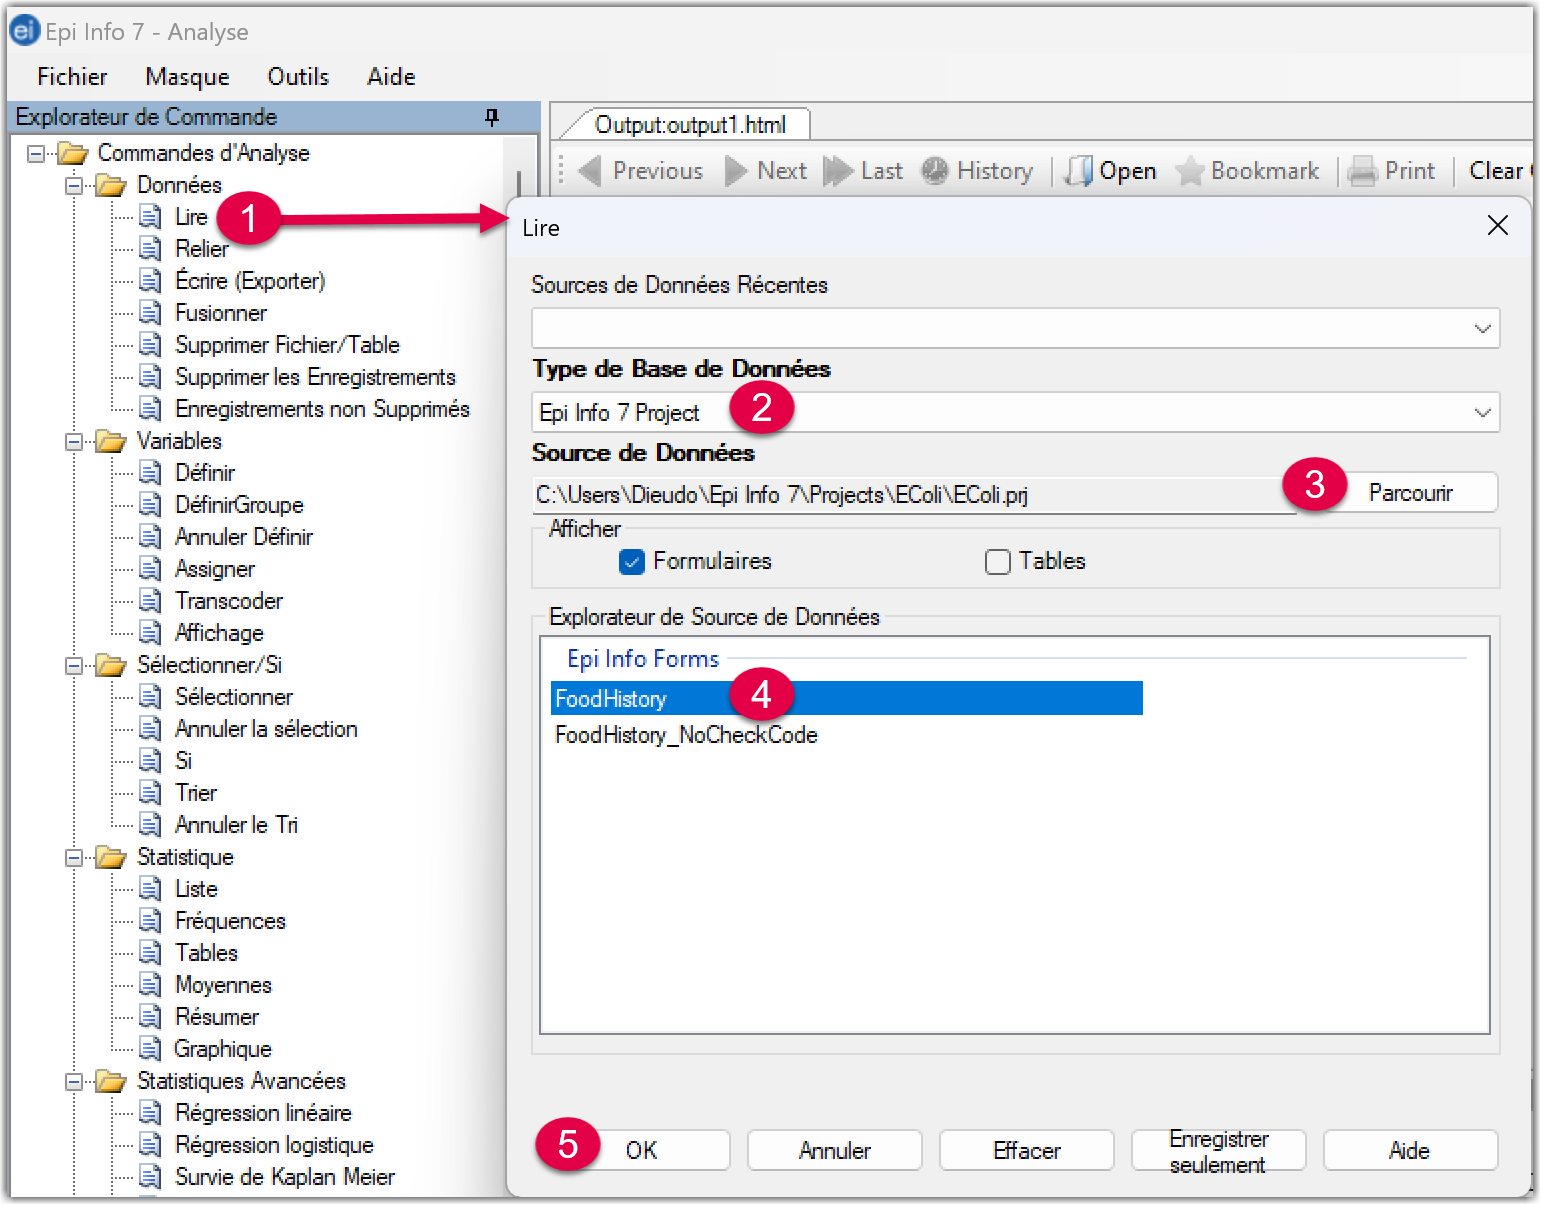
\includegraphics[width=\linewidth,height=0.4\textheight,keepaspectratio]{img/Classique/commandeRead}
	\caption{Utilisation de la commande Lire (Read) pour importer un fichier de données}
	\label{fig:commanderead}
\end{figure}

À l'issue de cette étape, nous obtenons la fenêtre de la \autoref{fig:fenetreapresimport}.

\begin{figure}[H]
	\centering
	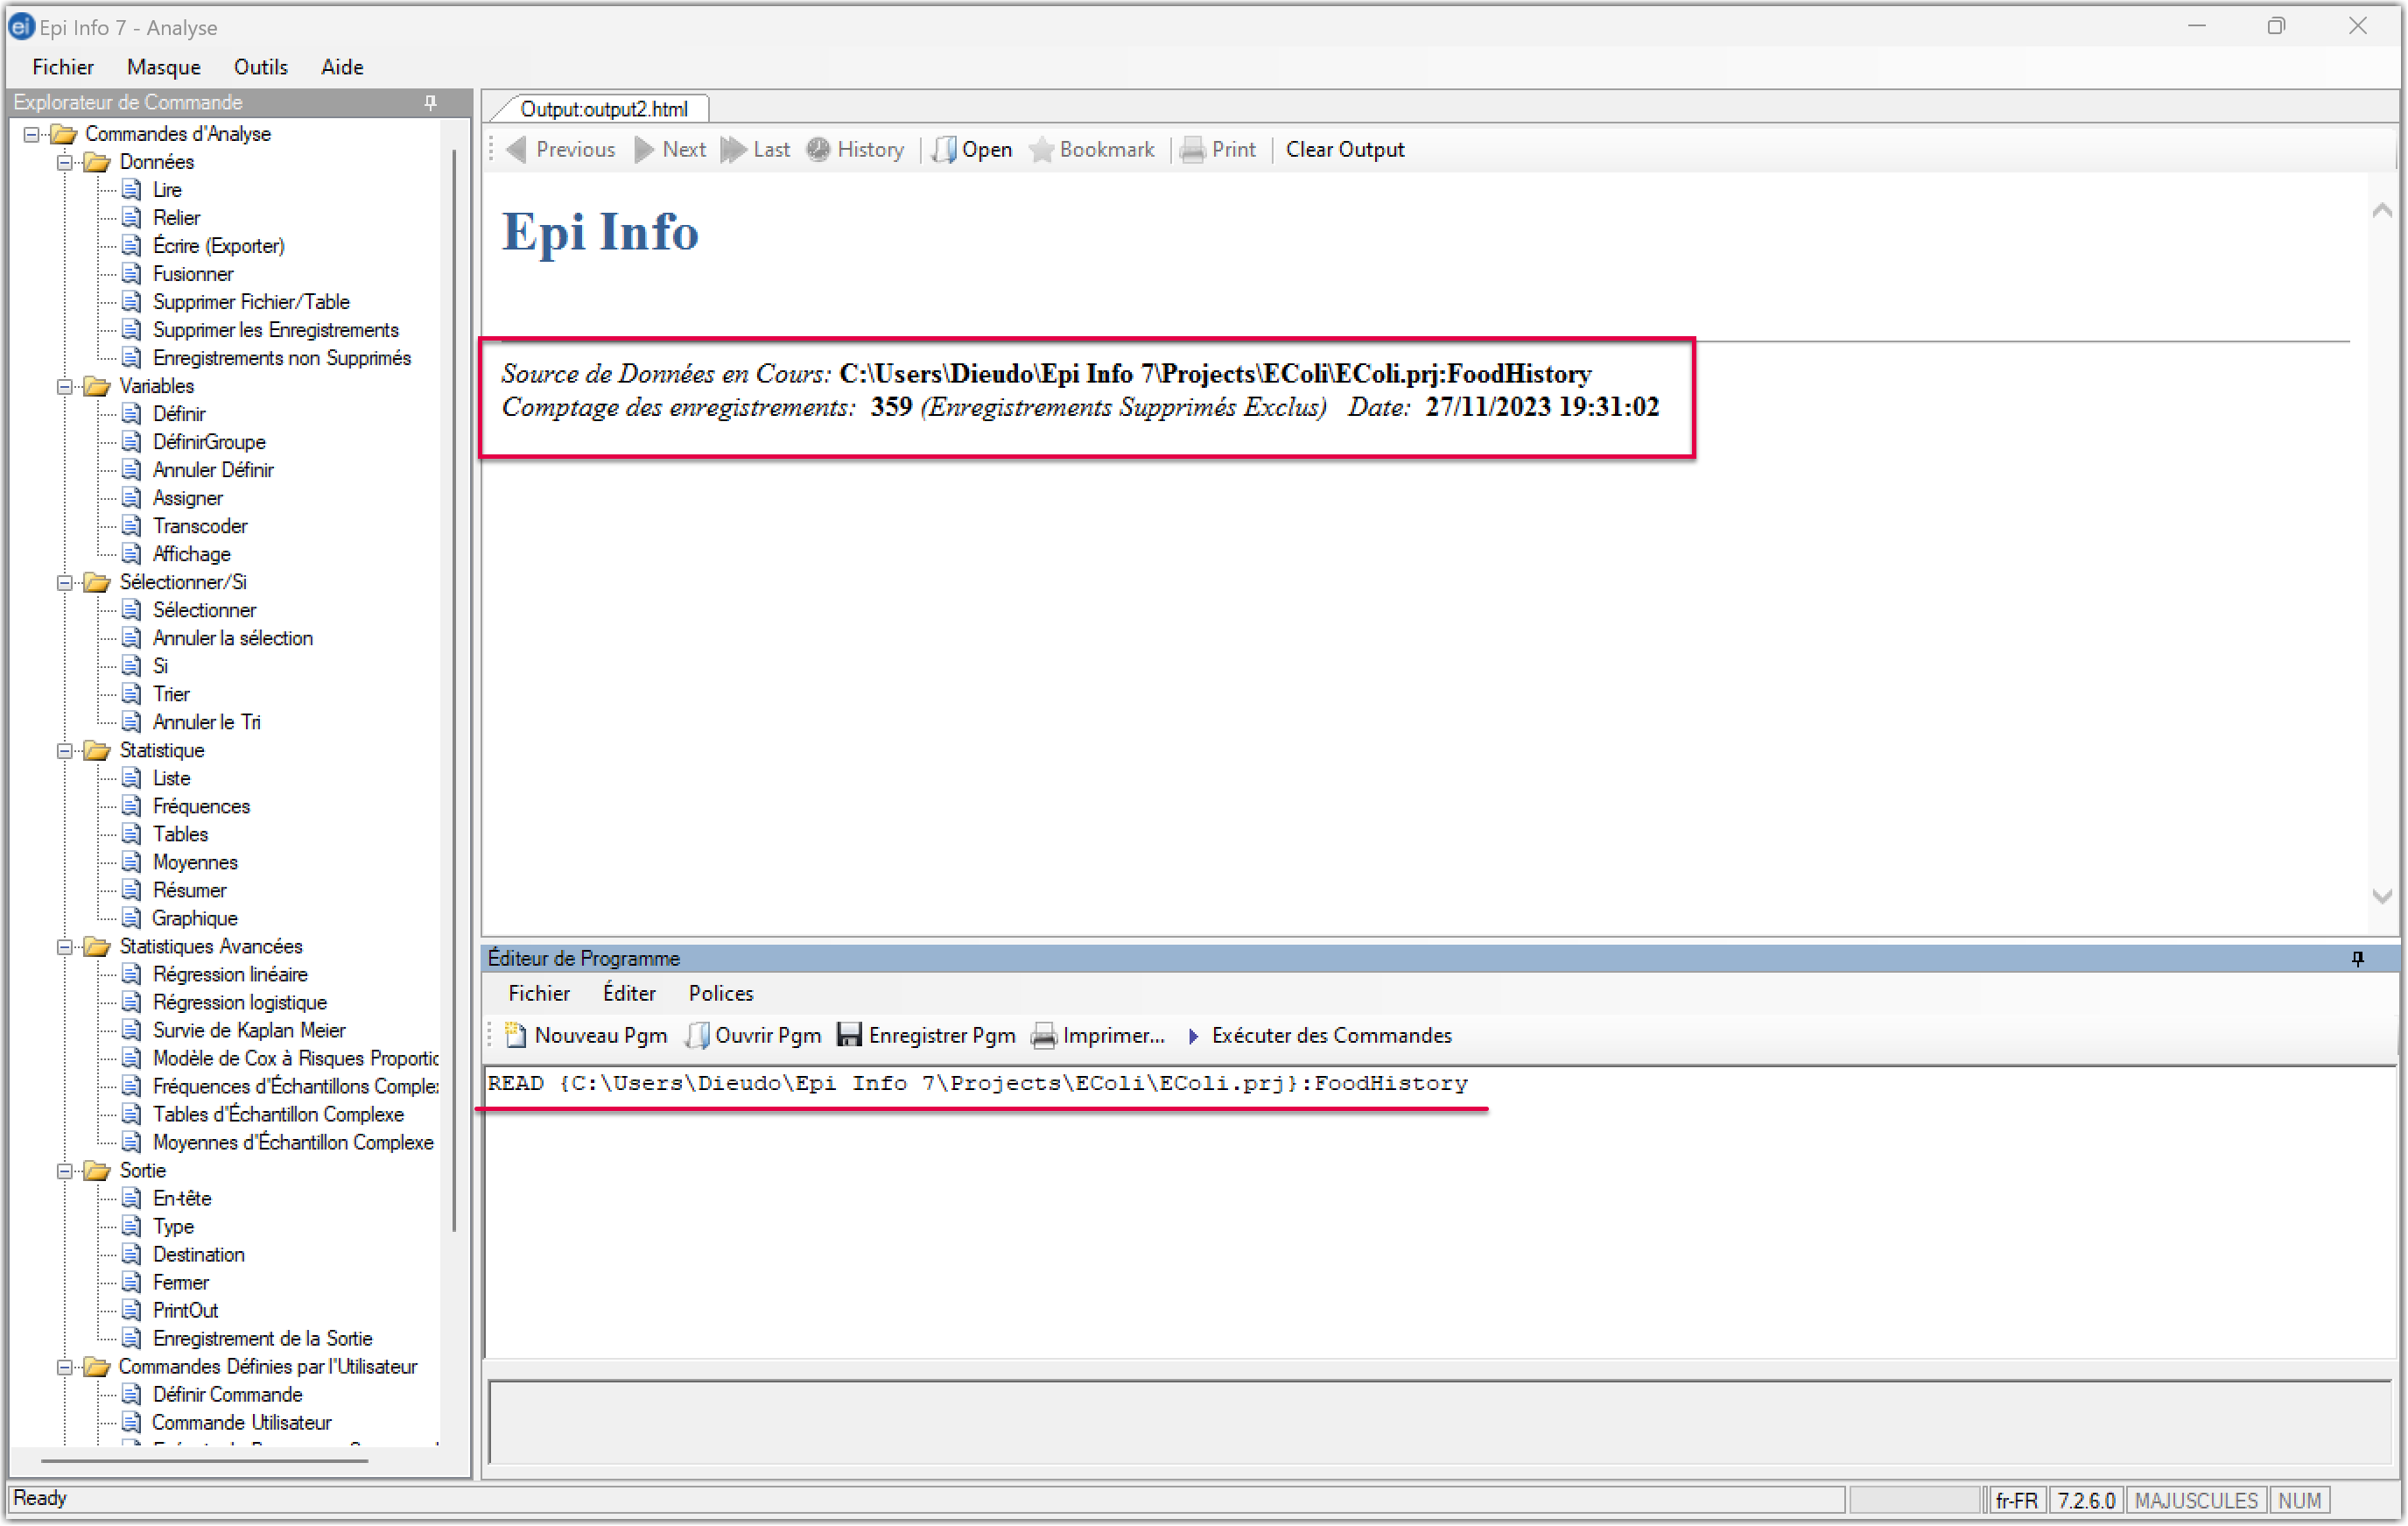
\includegraphics[width=\linewidth,height=0.4\textheight,keepaspectratio]{img/Classique/fenetreApresImport}
	\caption{Fenêtre du module Classique après l'import des données}
	\label{fig:fenetreapresimport}
\end{figure}

\begin{mybox}[colbacktitle=NOTE]{\faInfoCircle{} À RETENIR}
	Pour ouvrir un fichier Excel ou CSV, suivez la même procédure en choisissant Microsoft Excel ou \kw{CSV file} dans \kw{Type de base de données}.
\end{mybox}

Remarquez que la commande qui a servi à importer les données est écrite dans l'éditeur de programme (\autoref{lst:read}).

\begin{tcolorbox}[drop lifted shadow]
	\begin{lstlisting}[language=EPIscript, style=mystyle, caption={Commande d'import de la base EColi}, label=lst:read]
READ {C:\Users\Dieudo\Epi Info 7\Projects\EColi\EColi.prj}:FoodHistory
	\end{lstlisting}
\end{tcolorbox}

\section{Enregistrer et rouvrir un programme}

L'un des grands avantages du module \module{classique} est qu'il permet d'enregistrer les commandes de l'analyse dans un programme. On peut ainsi refaire toute l'analyse en un clic, ce qui facilite la reproductibilité, comme avec des logiciels de renom tels que \textsc{r}, \textsc{python} ou \textsc{stata}.

Pour enregistrer le programme (\autoref{fig:enregistrerprogramme}, page~\pageref{fig:enregistrerprogramme}) :

\begin{itemize}
	\item Cliquer sur \kw{Enregistrer Pgm}. Une fenêtre s'ouvre ;
	\item Dans la fenêtre \kw{Save Program}, au niveau de \kw{Fichier Projet}, cliquer sur le bouton à trois points situé à droite pour choisir le projet ;
	\item Dans \kw{Programme}, écrire le nom du programme, ici \var{prg\_ECOLI} ;
	\item Ajouter le nom de l'auteur du programme (votre nom) ;
	\item Ajouter éventuellement un commentaire dans \kw{Commentaires}, par exemple \question{Script Epi Info d'analyse de la base de données ECOLI} ;
	\item Valider par \kw{OK}.
\end{itemize}

\begin{figure}[H]
	\centering
	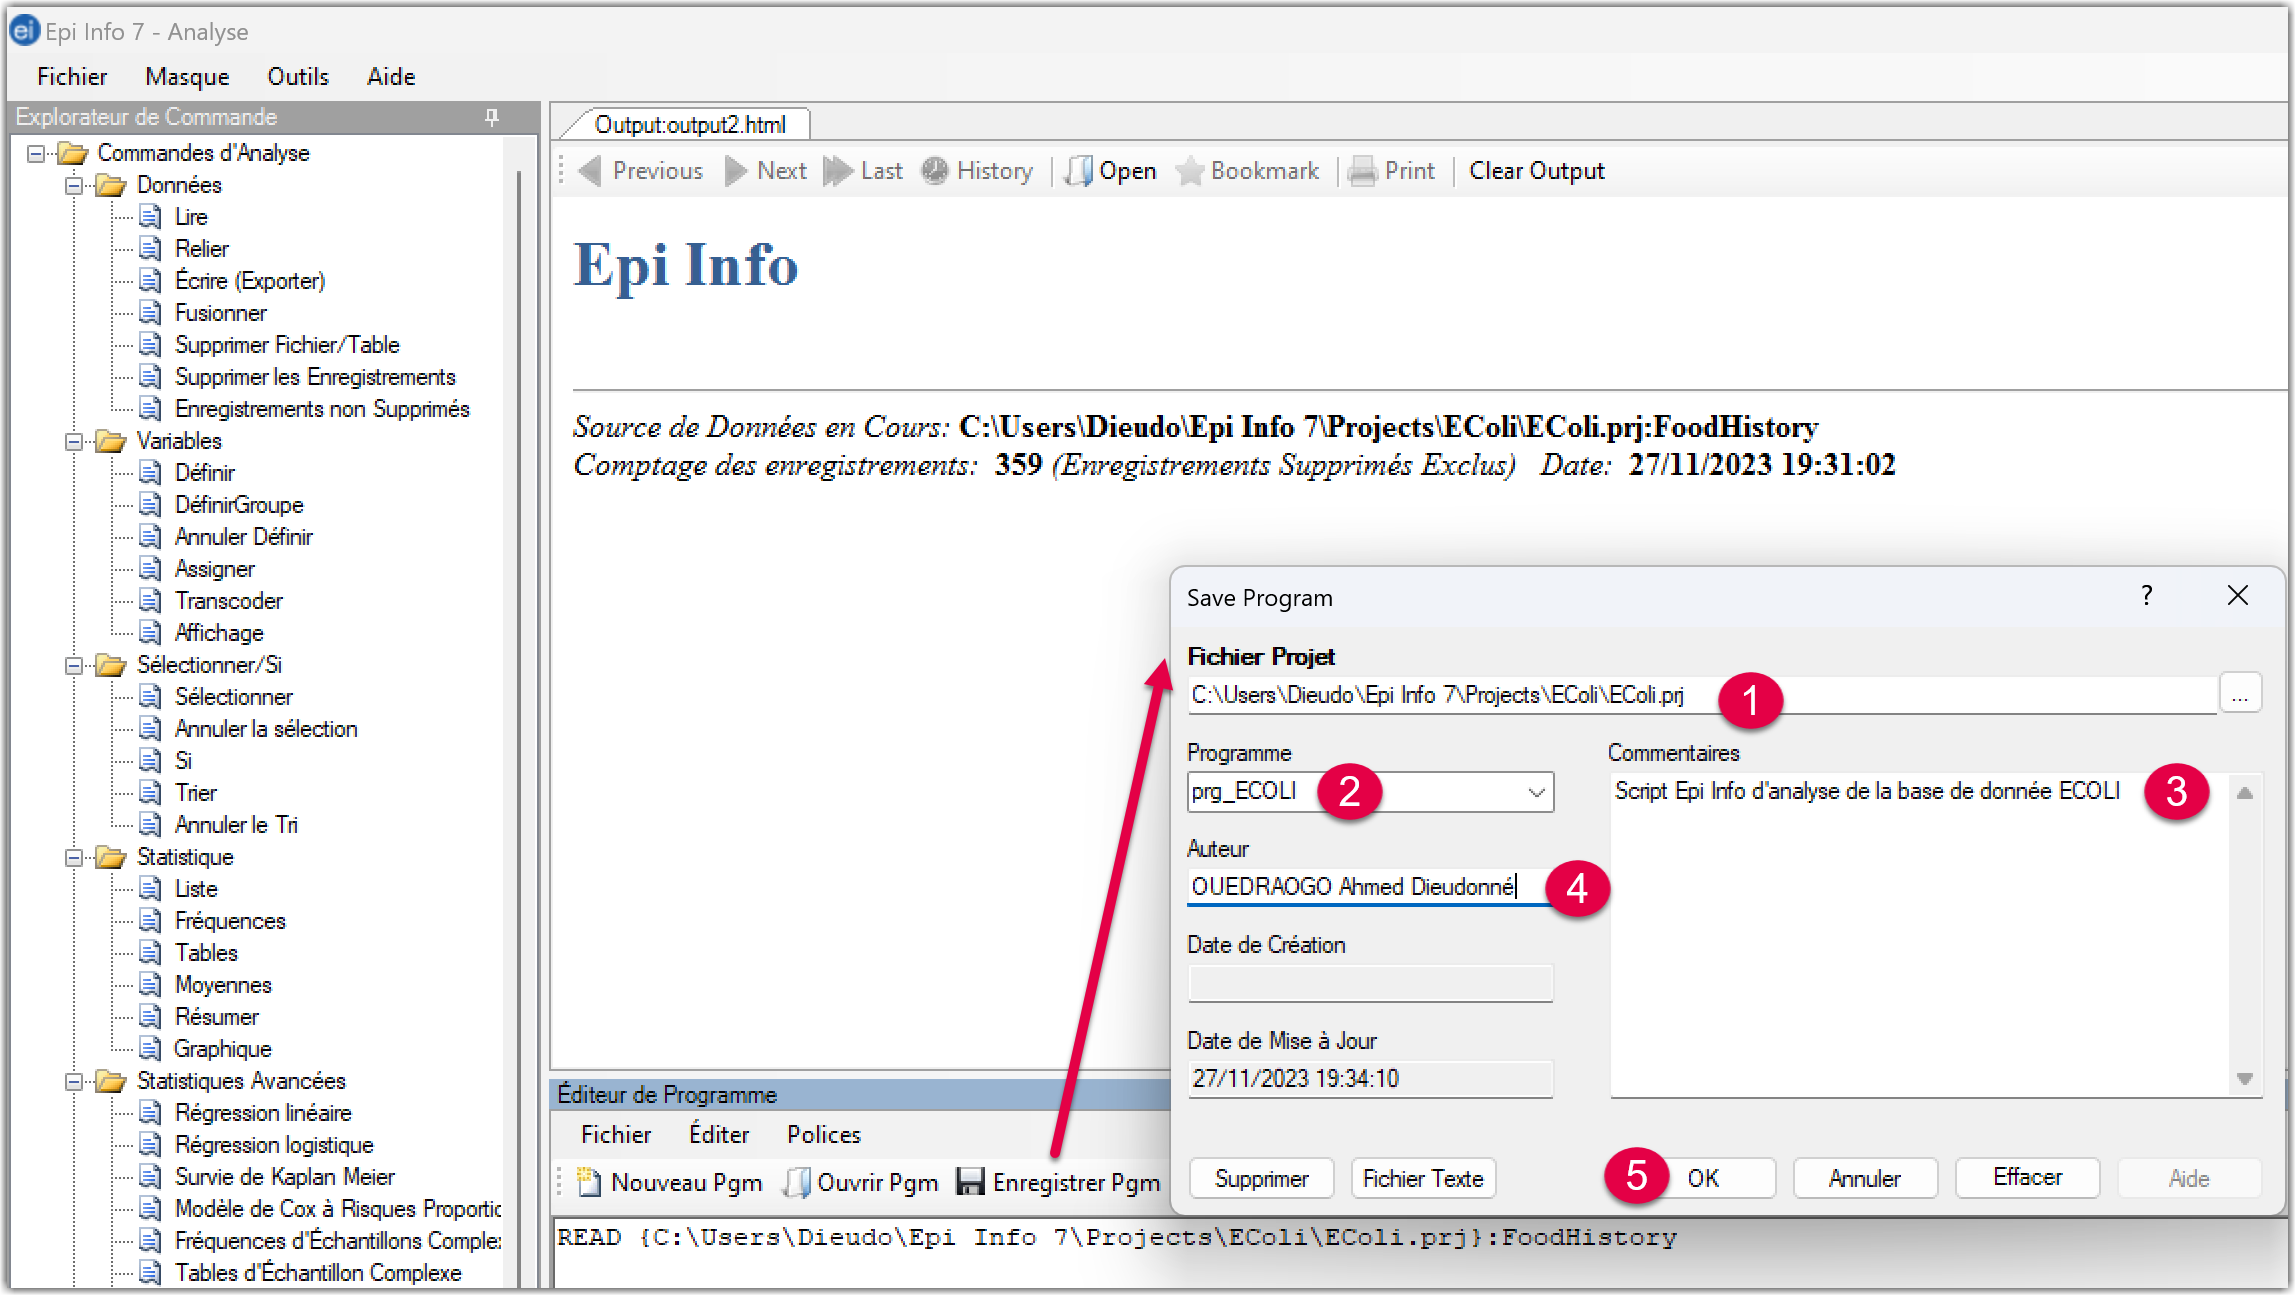
\includegraphics[width=\linewidth,height=0.4\textheight,keepaspectratio]{img/Classique/enregistrerProgramme}
	\caption{Enregistrer un programme}
	\label{fig:enregistrerprogramme}
\end{figure}

Au fur et à mesure de l'analyse, cliquez régulièrement sur \kw{Enregistrer Pgm} pour sauvegarder le programme.

Pour reprendre l'analyse après avoir quitté Epi Info, cliquer sur \kw{Ouvrir Pgm}, choisir le projet puis le programme contenant les commandes. Il faut ensuite exécuter les commandes souhaitées, en commençant obligatoirement par la commande \commande{READ} qui importe les données. Pour cela, sélectionnez les lignes voulues dans l'éditeur de programme puis cliquez sur \kw{Exécuter des Commandes}, dans la barre d'outils de l'éditeur.

\begin{mybox}[colbacktitle=TIP]{\faLightbulb{} CONSEIL}
Comme dans le code de contrôle, une ligne qui commence par \commande{//} est un commentaire : elle n'est pas exécutée. Commentez votre programme pour vous y retrouver plus tard.
\end{mybox}

\section{Explorer les données}

Avant de commencer l'analyse, il est utile de vérifier le type des variables. Pour cela, cliquer sur la commande \kw{Affichage} de la section \kw{Variables}, puis choisir d'afficher les variables de la base. La commande \commande{DISPLAY DBVARIABLES} s'écrit dans l'éditeur de programme. Son exécution affiche le dictionnaire des données sous forme de tableau : pour chaque variable, son nom, la question correspondante, son type, etc. C'est une vue d'ensemble de la base.

La commande \kw{Liste} de la section \kw{Statistique} affiche quant à elle les données brutes, enregistrement par enregistrement. Elle permet de voir la structure des données. Le symbole \commande{*} désigne toutes les variables ; on peut aussi n'en lister que quelques-unes.

\begin{tcolorbox}[drop lifted shadow]
	\begin{lstlisting}[language=EPIscript, style=mystyle, caption={Explorer les données}, label=lst:explorer]
// Dictionnaire des données de la base
DISPLAY DBVARIABLES
// Liste de toutes les variables
LIST *
// Liste de quelques variables seulement
LIST Age Sex ILL
	\end{lstlisting}
\end{tcolorbox}

\section{Statistique descriptive}

\subsection{Décrire une variable qualitative}

Pour décrire une variable qualitative, nous utilisons le \og tableau de fréquences \fg{}, qui présente l'effectif et le pourcentage de chaque modalité. Pour l'obtenir, cliquer sur \kw{Fréquences} dans la section \kw{Statistiques}, sélectionner la variable dans la liste déroulante \kw{Fréquence de}, puis cliquer sur \kw{OK}.

Pour la variable \var{ILL}, nous retrouvons les résultats du chapitre précédent : 276 malades (76,88~\%) et 83 non-malades (23,12~\%). Le module \module{classique} ajoute l'intervalle de confiance à 95~\% de chaque pourcentage.

Pour stratifier la fréquence selon une autre variable, comme le sexe, il suffit de choisir cette variable dans la liste \kw{Stratifier par} de la même fenêtre. La commande s'écrit alors avec l'option \commande{STRATAVAR} (\autoref{lst:freq}).

\begin{tcolorbox}[drop lifted shadow]
	\begin{lstlisting}[language=EPIscript, style=mystyle, caption={Tableaux de fréquences}, label=lst:freq]
// Fréquence de la variable ILL
FREQ ILL
// Fréquence de ILL stratifiée selon le sexe
FREQ ILL STRATAVAR=Sex
	\end{lstlisting}
\end{tcolorbox}

\subsection{Décrire une variable quantitative}

Pour décrire une variable quantitative, nous utilisons la commande \kw{Moyennes} de la section \kw{Statistique}. Sélectionner la variable dans la liste \kw{Moyennes de}, ici \var{Age}, puis valider par \kw{OK}. Le résultat donne, comme dans le Tableau de bord, l'effectif, la somme, la moyenne, la variance, l'écart-type, le minimum, les quartiles, la médiane, le maximum et le mode.

Pour comparer l'âge selon le sexe, choisir la variable \var{Sex} dans la liste \kw{Croisé par}. Epi Info affiche alors les statistiques de l'âge pour chaque sexe et réalise un test de comparaison des moyennes : l'analyse de variance (ANOVA) et, en complément, le test non paramétrique de Kruskal-Wallis, à privilégier lorsque la distribution de la variable n'est pas normale.

\begin{tcolorbox}[drop lifted shadow]
	\begin{lstlisting}[language=EPIscript, style=mystyle, caption={Paramètres de position et de dispersion}, label=lst:means]
// Statistiques descriptives de l'âge
MEANS Age
// Âge selon le sexe, avec test de comparaison
MEANS Age Sex
	\end{lstlisting}
\end{tcolorbox}

\section{Créer et recoder des variables}

\subsection{Recoder une variable}

Comme dans le Tableau de bord, nous pouvons recoder l'âge en tranches d'âge. Dans le module \module{classique}, cela se fait en deux temps :
\begin{enumerate}
	\item Créer la nouvelle variable avec la commande \kw{Définir} (\commande{DEFINE}) de la section \kw{Variables} ;
	\item Remplir cette variable avec la commande \kw{Transcoder} (\commande{RECODE}), en indiquant la variable source (\var{Age}), la variable de destination (\var{tranche\_age}) et les intervalles de recodage.
\end{enumerate}

\begin{tcolorbox}[drop lifted shadow]
	\begin{lstlisting}[language=EPIscript, style=mystyle, caption={Recodage de l'âge en tranches d'âge}, label=lst:recode]
DEFINE tranche_age TEXTINPUT
RECODE Age TO tranche_age
	LOVALUE - 14 = "0-14 ans"
	15 - 29 = "15-29 ans"
	30 - 44 = "30-44 ans"
	45 - 59 = "45-59 ans"
	60 - HIVALUE = "60 ans et plus"
END
FREQ tranche_age
	\end{lstlisting}
\end{tcolorbox}

\begin{mybox}[colbacktitle=CAUTION]{\faFire{} AVERTISSEMENT}
Les variables créées avec \commande{DEFINE} n'existent que pendant la session d'analyse : elles ne sont pas enregistrées dans la base. Elles seront recréées chaque fois que vous réexécuterez votre programme ; c'est une raison de plus pour bien l'enregistrer.
\end{mybox}

\subsection{Calculer une variable avec Assigner}

La commande \kw{Assigner} (\commande{ASSIGN}) de la section \kw{Variables} affecte à une variable le résultat d'un calcul, comme dans le code de contrôle (chapitre~\ref{codeValidation}). Créons par exemple l'âge en mois à partir de l'âge en années :
\begin{enumerate}
	\item Créer la variable \var{age\_mois} avec la commande \kw{Définir}, en choisissant le type numérique ;
	\item Cliquer sur \kw{Assigner}, choisir la variable \var{age\_mois} et écrire l'expression \var{Age * 12} ;
	\item Valider par \kw{OK}.
\end{enumerate}

\begin{tcolorbox}[drop lifted shadow]
	\begin{lstlisting}[language=EPIscript, style=mystyle, caption={Calcul d'une nouvelle variable}, label=lst:assignclassic]
DEFINE age_mois NUMERIC
ASSIGN age_mois = Age * 12
MEANS age_mois
	\end{lstlisting}
\end{tcolorbox}

\subsection{Créer une variable sous condition avec Si}

La commande \kw{Si} (\commande{IF}) de la section \kw{Sélectionner/Si} exécute une ou plusieurs commandes lorsqu'une condition est remplie, et éventuellement d'autres commandes dans le cas contraire (\commande{ELSE}). Elle sert souvent à créer une variable Oui/Non à partir d'une autre variable. Créons par exemple la variable \var{majeur}, qui vaut Oui si la personne a 18 ans ou plus :

\begin{tcolorbox}[drop lifted shadow]
	\begin{lstlisting}[language=EPIscript, style=mystyle, caption={Création d'une variable Oui/Non sous condition}, label=lst:ifclassic]
DEFINE majeur YN
IF Age >= 18 THEN
	ASSIGN majeur = (+)
ELSE
	ASSIGN majeur = (-)
END
FREQ majeur
	\end{lstlisting}
\end{tcolorbox}

Le type \commande{YN} crée une variable Oui/Non ; \commande{NUMERIC} crée une variable numérique, \commande{TEXTINPUT} une variable texte et \commande{DATEFORMAT} une variable date.

\begin{mybox}[colbacktitle=TIP]{\faLightbulb{} CONSEIL}
Prenez l'habitude de vérifier chaque nouvelle variable par une commande \commande{FREQ} ou \commande{MEANS}, comme dans les exemples ci-dessus. Vous repérerez ainsi immédiatement une erreur de recodage ou une condition mal écrite.
\end{mybox}

\section{Sélectionner une partie des données}

La commande \kw{Sélectionner} (\commande{SELECT}) de la section \kw{Sélectionner/Si} joue le même rôle que les filtres du Tableau de bord : les commandes suivantes ne portent que sur les enregistrements qui remplissent la condition. La commande \kw{Annuler la sélection} (\commande{CANCEL SELECT}) revient à l'ensemble des données.

\begin{tcolorbox}[drop lifted shadow]
	\begin{lstlisting}[language=EPIscript, style=mystyle, caption={Sélection des malades âgés de 25 à 35 ans}, label=lst:select]
SELECT ILL = (+) AND Age >= 25 AND Age <= 35
LIST Age Sex ILL
CANCEL SELECT
	\end{lstlisting}
\end{tcolorbox}

\begin{mybox}[colbacktitle=CAUTION]{\faFire{} AVERTISSEMENT}
Une sélection reste active jusqu'à ce qu'elle soit annulée. Vérifiez toujours le nombre d'enregistrements affiché dans les résultats avant d'interpréter une analyse.
\end{mybox}

\section{Trier les données}

La commande \kw{Trier} (\commande{SORT}) de la section \kw{Sélectionner/Si} classe les enregistrements selon une ou plusieurs variables, par ordre croissant ou décroissant. Le tri est utile avant une commande \commande{LIST}, par exemple pour repérer les valeurs extrêmes. La commande \kw{Annuler le Tri} rétablit l'ordre initial.

\begin{tcolorbox}[drop lifted shadow]
	\begin{lstlisting}[language=EPIscript, style=mystyle, caption={Tri des enregistrements selon l'âge}, label=lst:sort]
SORT Age DESCENDING
LIST Age Sex ILL
	\end{lstlisting}
\end{tcolorbox}

\section{Les valeurs manquantes}

Une valeur manquante correspond à un champ resté vide lors de la saisie. Par défaut, Epi Info exclut les valeurs manquantes des calculs : dans la base EColi, la moyenne des âges porte ainsi sur 356 personnes et non sur 359, car trois âges ne sont pas renseignés. Dans les commandes, une valeur manquante s'écrit \commande{(.)}. On peut ainsi lister les enregistrements dont l'âge est manquant pour les vérifier :

\begin{tcolorbox}[drop lifted shadow]
	\begin{lstlisting}[language=EPIscript, style=mystyle, caption={Repérer les valeurs manquantes}, label=lst:missing]
SELECT Age = (.)
LIST *
CANCEL SELECT
	\end{lstlisting}
\end{tcolorbox}

\begin{mybox}[colbacktitle=IMPORTANT]{\faExclamationCircle{} IMPORTANT}
Comparez toujours l'effectif d'une analyse avec l'effectif total de la base. Un écart important signale des valeurs manquantes, qu'il faut décrire et discuter dans votre mémoire ou votre thèse.
\end{mybox}

\section{Croiser deux variables : le tableau 2x2}

La commande \kw{Tables} (\commande{TABLES}) de la section \kw{Statistique} croise deux variables qualitatives. Indiquer la variable d'exposition, ici \var{Icecream}, puis la variable de résultat, ici \var{ILL}, et valider par \kw{OK}.

\begin{tcolorbox}[drop lifted shadow]
	\begin{lstlisting}[language=EPIscript, style=mystyle, caption={Tableau 2x2 entre la crème glacée et la maladie}, label=lst:tables]
TABLES Icecream ILL
	\end{lstlisting}
\end{tcolorbox}

Pour un tableau 2x2, Epi Info affiche le tableau croisé, l'odds ratio et le risque relatif avec leurs intervalles de confiance à 95~\%, ainsi que les tests du chi carré et le test exact de Fisher. Ils s'interprètent comme au chapitre précédent (section~\ref{tableau2x2}, page~\pageref{tableau2x2}) : une association est statistiquement significative si la valeur \textit{p} est inférieure à 0,05, ou si l'intervalle de confiance ne contient pas 1. On retrouve ici exactement les résultats obtenus avec le Tableau de bord.

\subsection{Tableau stratifié et facteur de confusion}

L'option \commande{STRATAVAR}, que l'on obtient en choisissant une variable dans la liste \kw{Stratifier par}, réalise un tableau 2x2 pour chaque modalité d'une troisième variable. Epi Info calcule alors, en plus des résultats de chaque strate, un odds ratio et un risque relatif \terme{ajustés} sur cette variable, selon la méthode de Mantel-Haenszel.

\begin{tcolorbox}[drop lifted shadow]
	\begin{lstlisting}[language=EPIscript, style=mystyle, caption={Tableau 2x2 stratifié selon le sexe}, label=lst:stratavar]
TABLES Icecream ILL STRATAVAR=Sex
	\end{lstlisting}
\end{tcolorbox}

Si la mesure ajustée est proche de la mesure brute, le sexe n'est pas un facteur de confusion de l'association entre la crème glacée et la maladie. Si elle s'en écarte nettement (de plus de 10 à 20~\% selon l'usage courant), le sexe est un facteur de confusion et c'est la mesure ajustée qu'il faut retenir. Si les mesures diffèrent fortement d'une strate à l'autre, on parle de modification d'effet : il faut alors présenter les résultats strate par strate.

\subsection{Tableau MxN}

Lorsque l'une des variables a plus de deux modalités, comme la variable \var{tranche\_age} créée plus haut, la commande \commande{TABLES} produit un tableau MxN. Epi Info calcule alors le test du chi carré, qui indique si la répartition de la maladie diffère selon les tranches d'âge.

\begin{tcolorbox}[drop lifted shadow]
	\begin{lstlisting}[language=EPIscript, style=mystyle, caption={Tableau croisé des tranches d'âge et de la maladie}, label=lst:mxn]
TABLES tranche_age ILL
	\end{lstlisting}
\end{tcolorbox}

\begin{mybox}[colbacktitle=CAUTION]{\faFire{} AVERTISSEMENT}
Le test du chi carré n'est valide que si les effectifs attendus sont suffisamment grands (en règle générale au moins 5 dans chaque case). Lorsque ce n'est pas le cas, Epi Info le signale : regroupez alors des modalités ou utilisez le test exact de Fisher pour un tableau 2x2.
\end{mybox}

\section{Représentations graphiques}

La commande \kw{Graphique} de la section \kw{Statistique} réalise des graphiques sans quitter le module : diagrammes en barres, en secteurs, histogrammes, courbes, etc. Dans la fenêtre qui s'ouvre, choisir le type de graphique, la variable à représenter et, si besoin, une variable de regroupement, puis valider par \kw{OK}. Le graphique s'affiche dans une fenêtre séparée, d'où l'on peut l'enregistrer comme image. Comme pour le Tableau de bord, nous préférerons souvent réaliser les graphiques définitifs dans un tableur.

\section{Exporter et fusionner des données}

\subsection{Exporter des données}

La commande \kw{Écrire (Exporter)} de la section \kw{Données} enregistre les données, avec les variables créées pendant l'analyse, dans un autre fichier : base Epi Info, classeur Excel ou fichier CSV. Dans la fenêtre qui s'ouvre, choisir les variables à exporter (ou toutes les variables), le format et l'emplacement du fichier, puis valider par \kw{OK}. Si une sélection est active, seuls les enregistrements sélectionnés sont exportés.

\subsection{Fusionner deux bases}

Lorsque plusieurs enquêteurs ont saisi des données sur le même questionnaire, il faut les rassembler dans une seule base. La commande \kw{Fusionner} de la section \kw{Données} réunit la base en cours, ouverte avec \commande{READ}, et une seconde base. Elle peut ajouter les enregistrements de la seconde base à la suite de ceux de la première, ou compléter les enregistrements existants à l'aide d'une variable d'identification commune.

\begin{mybox}[colbacktitle=NOTE]{\faInfoCircle{} À RETENIR}
La fusion n'est simple que si toutes les bases proviennent du même questionnaire. C'est l'intérêt d'envoyer à tous les enquêteurs le même modèle de projet (section~\ref{modeleProjet}, page~\pageref{modeleProjet}).
\end{mybox}

\section{Aller plus loin}

\subsection{Enregistrer les résultats}

Par défaut, les résultats s'affichent dans la fenêtre de résultats et sont perdus à la fermeture du module. La commande \kw{Destination} de la section \kw{Sortie} (\commande{ROUTEOUT}) envoie les résultats dans un fichier HTML, que l'on peut ouvrir dans un navigateur, imprimer ou copier dans un traitement de texte. La commande \kw{Fermer} de la même section (\commande{CLOSEOUT}) ferme ce fichier.

\begin{tcolorbox}[drop lifted shadow]
	\begin{lstlisting}[language=EPIscript, style=mystyle, caption={Enregistrer les résultats dans un fichier}, label=lst:routeout]
ROUTEOUT "C:\Users\Dieudo\Documents\resultats_EColi.html" REPLACE
FREQ ILL
MEANS Age Sex
TABLES Icecream ILL
CLOSEOUT
	\end{lstlisting}
\end{tcolorbox}

\subsection{Les statistiques avancées}

La section \kw{Statistiques Avancées} donne accès à des modèles plus complexes. Les plus utilisés sont :
\begin{itemize}
	\item la \terme{régression logistique} (\kw{Régression logistique}), lorsque la variable à expliquer est binaire (malade/non malade). Elle estime des odds ratios ajustés, c'est-à-dire l'effet propre de chaque facteur en tenant compte des autres, comme nous l'avons évoqué au chapitre précédent ;
	\item la \terme{régression linéaire} (\kw{Régression linéaire}), lorsque la variable à expliquer est quantitative (le poids, la pression artérielle\ldots) ;
	\item l'\terme{analyse de survie} (\kw{Survie de Kaplan Meier} et \kw{Modèle de Cox à Risques Proportionnels}), lorsque l'on s'intéresse au délai de survenue d'un événement, comme le décès ou la guérison.
\end{itemize}

Par exemple, pour mesurer l'effet de la crème glacée sur la maladie en tenant compte de l'âge, cliquer sur \kw{Régression logistique}, choisir \var{ILL} comme variable de résultat, \var{Icecream} et \var{Age} comme variables explicatives, puis valider par \kw{OK}.

\begin{tcolorbox}[drop lifted shadow]
	\begin{lstlisting}[language=EPIscript, style=mystyle, caption={Régression logistique}, label=lst:logistic]
LOGISTIC ILL = Icecream Age
	\end{lstlisting}
\end{tcolorbox}

Le résultat donne, pour chaque variable explicative, un odds ratio ajusté avec son intervalle de confiance à 95~\% et sa valeur \textit{p}, qui se lisent comme ceux d'un tableau 2x2.

Ces méthodes demandent de solides bases en biostatistique ; prenez le temps de les maîtriser avant de les utiliser pour votre mémoire ou votre thèse.

\section[Récapitulatif des commandes essentielles][Récapitulatif des commandes]{Récapitulatif des commandes essentielles}

Le \autoref{tab:commandesClassique} rassemble les commandes du module \module{classique} vues dans ce chapitre.

\begin{table}[H]
	\centering
	\caption{Commandes essentielles du module Classique}
	\label{tab:commandesClassique}
	\footnotesize
	\begin{tabular}{|l|>{\raggedright\arraybackslash}p{4cm}|>{\raggedright\arraybackslash}p{4.4cm}|}
		\hline
		\textbf{Commande} & \textbf{Bouton (section)} & \textbf{Rôle} \\
		\hline
		\commande{READ} & Lire (Données) & Ouvrir une base de données \\
		\commande{DISPLAY DBVARIABLES} & Affichage (Variables) & Afficher le dictionnaire des données \\
		\commande{LIST} & Liste (Statistique) & Lister les enregistrements \\
		\commande{FREQ} & Fréquences (Statistique) & Tableau de fréquences \\
		\commande{MEANS} & Moyennes (Statistique) & Statistiques d'une variable quantitative \\
		\commande{TABLES} & Tables (Statistique) & Tableau croisé, OR, RR, chi carré \\
		\commande{DEFINE} & Définir (Variables) & Créer une variable \\
		\commande{ASSIGN} & Assigner (Variables) & Calculer une variable \\
		\commande{RECODE} & Transcoder (Variables) & Recoder une variable \\
		\commande{IF} & Si (Sélectionner/Si) & Exécuter des commandes sous condition \\
		\commande{SELECT} & Sélectionner (Sélectionner/Si) & Filtrer les enregistrements \\
		\commande{SORT} & Trier (Sélectionner/Si) & Trier les enregistrements \\
		\commande{LOGISTIC} & Régression logistique & Odds ratios ajustés \\
		\commande{ROUTEOUT} & Destination (Sortie) & Enregistrer les résultats \\
		\hline
	\end{tabular}
\end{table}

\chapter{Module StatCalc}
\label{moduleStatcalc}
%\minitoc

\module{statcalc} est le module de calculatrices statistiques d'Epi Info 7. Contrairement aux modules \module{tableau de bord visuel} et \module{classique}, il ne travaille pas sur une base de données : on y saisit directement des chiffres. Il sert surtout à deux choses :
\begin{itemize}
	\item calculer la \terme{taille de l'échantillon} nécessaire avant une enquête, une étape obligatoire de tout protocole de recherche ;
	\item analyser rapidement un tableau dont on connaît déjà les effectifs, par exemple un tableau publié dans un article ou un rapport.
\end{itemize}

Dans le cadre d'un mémoire ou d'une thèse, le calcul de la taille de l'échantillon se fait au moment de la rédaction du protocole, avec votre directeur ou directrice de mémoire ou de thèse, et doit être justifié dans la partie méthodologie.

\section{Ouvrir le module StatCalc}

Pour ouvrir le module, cliquer sur \module{statcalc} dans la fenêtre d'accueil d'Epi Info (\autoref{fig:tableaudebord}, page~\pageref{fig:tableaudebord}). Une fenêtre s'ouvre avec la liste des calculatrices disponibles, réparties en deux groupes\footnote{Les libellés indiqués ici peuvent varier légèrement selon la version d'Epi Info et sa traduction française.} :

\begin{itemize}
	\item \kw{Taille de l'échantillon et puissance} :
	\begin{itemize}
		\item \kw{Enquête de population}, pour une enquête descriptive (estimer une prévalence, une proportion) ;
		\item \kw{Cohorte ou transversale}, pour comparer des exposés et des non-exposés ;
		\item \kw{Cas-témoins non appariés}, pour comparer des malades (cas) et des non-malades (témoins) ;
	\end{itemize}
	\item les calculatrices d'analyse :
	\begin{itemize}
		\item \kw{Tables (2 x 2, 2 x n)}, pour analyser un tableau croisé ;
		\item \kw{Chi carré pour tendance}, pour rechercher une relation dose-effet ;
		\item \kw{Poisson} et \kw{Binomial}, pour comparer un nombre ou une proportion observés à une valeur attendue.
	\end{itemize}
\end{itemize}

Chaque calculatrice affiche ses résultats au fur et à mesure de la saisie : il n'y a pas de bouton de validation. Modifiez un paramètre et observez immédiatement son effet sur le résultat.

\begin{mybox}[colbacktitle=NOTE]{\faInfoCircle{} À RETENIR}
Le calcul de la taille de l'échantillon repose sur des hypothèses (prévalence attendue, précision souhaitée, risque relatif attendu\ldots). Ces hypothèses doivent être tirées de la littérature ou d'une étude préliminaire, et citées dans votre protocole.
\end{mybox}

\section[Taille de l'échantillon pour une enquête de population][Échantillon : enquête de population]{Taille de l'échantillon pour une enquête de population}
\label{statcalcPopulation}

C'est le calcul le plus courant pour une enquête descriptive, par exemple pour estimer la proportion de personnes vaccinées contre la Covid-19 dans une ville. Cliquer sur \kw{Enquête de population}, puis renseigner les paramètres suivants :

\begin{enumerate}
	\item \kw{Taille de la population} : le nombre de personnes de la population étudiée. Si elle est très grande ou inconnue, laisser la valeur par défaut, 999\,999 ;
	\item \kw{Fréquence attendue} : la proportion que l'on s'attend à trouver, en pourcentage, tirée de la littérature. Si elle est inconnue, saisir 50~\%, la valeur qui donne l'échantillon le plus grand ;
	\item \kw{Marge d'erreur acceptable} : la précision souhaitée, c'est-à-dire la demi-largeur de l'intervalle de confiance. On choisit le plus souvent 5~\% ;
	\item \kw{Effet de plan} : laisser 1 pour un sondage aléatoire simple. Pour un sondage en grappes, on utilise généralement 2 ;
	\item \kw{Grappes} : le nombre de grappes, 1 pour un sondage aléatoire simple.
\end{enumerate}

Epi Info affiche alors la taille de l'échantillon pour plusieurs niveaux de confiance (80~\%, 90~\%, 95~\%, 99~\%, etc.). On retient en général la ligne correspondant à 95~\%. Le calcul repose sur la formule suivante :
\[
n = \frac{z^2 \times p\,(1-p)}{d^2}
\]
où $z$ vaut 1,96 pour un niveau de confiance de 95~\%, $p$ est la fréquence attendue et $d$ la marge d'erreur. Epi Info y ajoute une correction lorsque la population est petite, et multiplie le résultat par l'effet de plan.

Par exemple, avec une population de 999\,999 personnes, une fréquence attendue de 50~\%, une marge d'erreur de 5~\% et un effet de plan de 1, on obtient pour un niveau de confiance de 95~\% :
\[
n = \frac{1{,}96^2 \times 0{,}5 \times 0{,}5}{0{,}05^2} \approx 384 \text{ personnes.}
\]

\begin{mybox}[colbacktitle=TIP]{\faLightbulb{} CONSEIL}
Prévoyez toujours une marge pour les refus et les questionnaires inexploitables. Avec un taux de non-réponse attendu de 10~\%, il faut enquêter $384/(1-0{,}10) \approx 427$ personnes. Si l'enquête se fait en grappes avec un effet de plan de 2, l'échantillon double : $384 \times 2 = 768$ personnes avant la majoration pour non-réponse.
\end{mybox}

\section[Taille de l'échantillon pour une étude de cohorte ou transversale][Échantillon : cohorte ou transversale]{Taille de l'échantillon pour une étude de cohorte ou transversale}

Lorsque l'on veut comparer la fréquence d'une maladie entre des exposés et des non-exposés, il faut un échantillon suffisant pour mettre en évidence une différence si elle existe. Cliquer sur \kw{Cohorte ou transversale}, puis renseigner :

\begin{enumerate}
	\item \kw{Niveau de confiance bilatéral} : en général 95~\%, ce qui correspond à un risque $\alpha$ de 5~\% ;
	\item \kw{Puissance} : la probabilité de mettre en évidence la différence si elle existe, en général 80~\% (risque $\beta$ de 20~\%) ;
	\item \kw{Ratio (non exposés : exposés)} : le nombre de non-exposés pour un exposé, en général 1 ;
	\item \kw{Pourcentage de non-exposés avec le résultat} : la fréquence de la maladie attendue chez les non-exposés ;
	\item enfin, \kw{Pourcentage d'exposés avec le résultat}, ou de façon équivalente le \kw{Risque relatif} ou l'\kw{Odds ratio} que l'on souhaite pouvoir mettre en évidence. Ces trois cases sont liées : en remplir une met à jour les deux autres.
\end{enumerate}

Epi Info affiche le nombre d'exposés, de non-exposés et le total selon trois méthodes : \kw{Kelsey}, \kw{Fleiss} et \kw{Fleiss avec CC} (avec correction de continuité). Les résultats sont proches ; la méthode de Fleiss avec correction de continuité est la plus prudente, car elle donne l'échantillon le plus grand.

Par exemple, avec un niveau de confiance de 95~\%, une puissance de 80~\%, un ratio de 1, une fréquence de la maladie de 20~\% chez les non-exposés et de 40~\% chez les exposés (soit un risque relatif de 2), il faut environ 82 exposés et 82 non-exposés selon la méthode de Fleiss, un peu plus avec la correction de continuité.

\section[Taille de l'échantillon pour une étude cas-témoins][Échantillon : étude cas-témoins]{Taille de l'échantillon pour une étude cas-témoins}

Dans une étude cas-témoins, on compare l'exposition des malades (cas) à celle de non-malades (témoins). Cliquer sur \kw{Cas-témoins non appariés}. Les paramètres sont les mêmes que pour une cohorte, à deux différences près :
\begin{itemize}
	\item le ratio est le nombre de \kw{témoins pour un cas}. Prendre deux, trois ou quatre témoins par cas augmente la puissance lorsque les cas sont rares ; au-delà de quatre, le gain devient faible ;
	\item on renseigne le \kw{pourcentage de témoins exposés}, puis le pourcentage de cas exposés ou l'\kw{odds ratio} que l'on souhaite pouvoir mettre en évidence.
\end{itemize}

Epi Info affiche le nombre de cas, de témoins et le total selon les mêmes trois méthodes.

\begin{mybox}[colbacktitle=CAUTION]{\faFire{} AVERTISSEMENT}
Plus la différence que l'on cherche à mettre en évidence est petite (un risque relatif ou un odds ratio proche de 1), plus l'échantillon nécessaire est grand. Choisissez un effet attendu réaliste, tiré de la littérature, et non un effet arrangé pour obtenir un petit échantillon.
\end{mybox}

\section{Analyser un tableau 2x2}
\label{statcalcTables}

La calculatrice \kw{Tables (2 x 2, 2 x n)} réalise les mêmes calculs que le gadget Table MxN / 2x2 du Tableau de bord ou la commande \commande{TABLES} du module Classique, mais à partir des seuls effectifs. Pour l'utiliser, cliquer sur \kw{Tables (2 x 2, 2 x n)} et saisir les quatre effectifs $a$, $b$, $c$ et $d$ du tableau (\autoref{tab:2x2}, page~\pageref{tab:2x2}) : les exposés malades et non malades sur la première ligne, les non-exposés malades et non malades sur la deuxième.

Saisissons les effectifs de l'exemple de la crème glacée (section~\ref{tableau2x2}) : 69 et 5 sur la première ligne, 207 et 78 sur la deuxième. StatCalc affiche aussitôt l'odds ratio (5,20), le risque relatif (1,28), leurs intervalles de confiance à 95~\%, les tests du chi carré et le test exact de Fisher : ce sont les résultats obtenus avec le Tableau de bord.

\begin{mybox}[colbacktitle=TIP]{\faLightbulb{} CONSEIL}
Cette calculatrice est très pratique pour vérifier un résultat publié dans un article, ou pour analyser un tableau quand on n'a pas accès à la base de données. StatCalc permet aussi de saisir plusieurs tableaux 2x2 (une strate par tableau) pour obtenir un odds ratio ajusté de Mantel-Haenszel.
\end{mybox}

\section{Les autres calculatrices}

\paragraph{Chi carré pour tendance} Cette calculatrice recherche une relation dose-effet : le risque de maladie augmente-t-il régulièrement avec le niveau d'exposition (par exemple avec le nombre de cigarettes fumées par jour) ? Pour chaque niveau d'exposition, on saisit un score, le nombre de cas et le nombre de témoins. Epi Info calcule un odds ratio pour chaque niveau, par rapport au premier, et le chi carré de tendance avec sa valeur \textit{p}.

\paragraph{Poisson} Cette calculatrice compare un nombre d'événements observé à un nombre attendu, lorsque l'événement est rare. Par exemple : on observe 12 cas d'une maladie dans un district où l'on en attend 5 d'après les années précédentes. Cet excès peut-il être dû au hasard ? Epi Info donne la probabilité d'observer au moins 12 cas si le nombre attendu est 5.

\paragraph{Binomial} Cette calculatrice compare une proportion observée à une proportion attendue. Par exemple : sur 50 enfants vaccinés, 8 ont présenté un effet indésirable, alors que la fréquence attendue est de 5~\%. Epi Info donne la probabilité d'observer un tel résultat si la fréquence réelle est bien de 5~\%.

\begin{mybox}[colbacktitle=NOTE]{\faInfoCircle{} À RETENIR}
\begin{itemize}[label=\ding{97}, font=\color{NOTE}]
	\item Avant l'enquête : \kw{Enquête de population} pour une étude descriptive, \kw{Cohorte ou transversale} ou \kw{Cas-témoins non appariés} pour une étude analytique ;
	\item Après l'enquête, ou à partir d'un tableau publié : \kw{Tables (2 x 2, 2 x n)}, \kw{Chi carré pour tendance}, \kw{Poisson} et \kw{Binomial}.
\end{itemize}
\end{mybox}

\chapter*{Conclusion}
\label{conclusion}
\addcontentsline{toc}{chapter}{Conclusion}
\markboth{Conclusion}{Conclusion}

Au fil de ce livre, nous avons parcouru toutes les étapes d'une enquête avec Epi Info 7 : concevoir un questionnaire robuste, le sécuriser avec le code de contrôle, saisir les données, puis les analyser avec le \module{tableau de bord visuel} et le module \module{classique}. Avec \module{statcalc}, nous avons aussi vu comment calculer la taille d'un échantillon avant même de commencer la collecte.

Si vous ne deviez retenir que quelques principes, ce seraient ceux-ci :
\begin{itemize}[label=\ding{97}, font=\color{EPIB}]
	\item une bonne analyse commence par un bon questionnaire : des noms de variables clairs, les bons types de champs et des contrôles de saisie ;
	\item testez toujours le questionnaire avant la collecte, puis ne modifiez plus sa structure ;
	\item vérifiez l'effectif de chaque analyse, surtout lorsqu'un filtre ou une sélection est actif ;
	\item enregistrez vos programmes d'analyse : ils rendent votre travail reproductible ;
	\item une association statistiquement significative ne prouve pas un lien de causalité.
\end{itemize}

Epi Info n'est qu'un outil. Ce qui donne de la valeur à vos résultats, c'est la rigueur de votre démarche, de la conception du protocole à l'interprétation des chiffres. Une fois ces bases acquises, vous pourrez aborder sereinement des analyses plus avancées, ou d'autres logiciels comme \textsc{r} ou \textsc{stata}.

Je vous souhaite de belles enquêtes et de bonnes analyses.

\bigskip
\begin{flushright}
	\textit{OUEDRAOGO Ahmed Dieudonné}\\
	\textit{2026}
\end{flushright}

\end{document}
